\documentclass[twoside]{book}

% Packages required by doxygen
\usepackage{fixltx2e}
\usepackage{calc}
\usepackage{doxygen}
\usepackage[export]{adjustbox} % also loads graphicx
\usepackage{graphicx}
\usepackage[utf8]{inputenc}
\usepackage{makeidx}
\usepackage{multicol}
\usepackage{multirow}
\PassOptionsToPackage{warn}{textcomp}
\usepackage{textcomp}
\usepackage[nointegrals]{wasysym}
\usepackage[table]{xcolor}

% Font selection
\usepackage[T1]{fontenc}
\usepackage[scaled=.90]{helvet}
\usepackage{courier}
\usepackage{amssymb}
\usepackage{sectsty}
\renewcommand{\familydefault}{\sfdefault}
\allsectionsfont{%
  \fontseries{bc}\selectfont%
  \color{darkgray}%
}
\renewcommand{\DoxyLabelFont}{%
  \fontseries{bc}\selectfont%
  \color{darkgray}%
}
\newcommand{\+}{\discretionary{\mbox{\scriptsize$\hookleftarrow$}}{}{}}

% Page & text layout
\usepackage{geometry}
\geometry{%
  a4paper,%
  top=2.5cm,%
  bottom=2.5cm,%
  left=2.5cm,%
  right=2.5cm%
}
\tolerance=750
\hfuzz=15pt
\hbadness=750
\setlength{\emergencystretch}{15pt}
\setlength{\parindent}{0cm}
\setlength{\parskip}{3ex plus 2ex minus 2ex}
\makeatletter
\renewcommand{\paragraph}{%
  \@startsection{paragraph}{4}{0ex}{-1.0ex}{1.0ex}{%
    \normalfont\normalsize\bfseries\SS@parafont%
  }%
}
\renewcommand{\subparagraph}{%
  \@startsection{subparagraph}{5}{0ex}{-1.0ex}{1.0ex}{%
    \normalfont\normalsize\bfseries\SS@subparafont%
  }%
}
\makeatother

% Headers & footers
\usepackage{fancyhdr}
\pagestyle{fancyplain}
\fancyhead[LE]{\fancyplain{}{\bfseries\thepage}}
\fancyhead[CE]{\fancyplain{}{}}
\fancyhead[RE]{\fancyplain{}{\bfseries\leftmark}}
\fancyhead[LO]{\fancyplain{}{\bfseries\rightmark}}
\fancyhead[CO]{\fancyplain{}{}}
\fancyhead[RO]{\fancyplain{}{\bfseries\thepage}}
\fancyfoot[LE]{\fancyplain{}{}}
\fancyfoot[CE]{\fancyplain{}{}}
\fancyfoot[RE]{\fancyplain{}{\bfseries\scriptsize Generated by Doxygen }}
\fancyfoot[LO]{\fancyplain{}{\bfseries\scriptsize Generated by Doxygen }}
\fancyfoot[CO]{\fancyplain{}{}}
\fancyfoot[RO]{\fancyplain{}{}}
\renewcommand{\footrulewidth}{0.4pt}
\renewcommand{\chaptermark}[1]{%
  \markboth{#1}{}%
}
\renewcommand{\sectionmark}[1]{%
  \markright{\thesection\ #1}%
}

% Indices & bibliography
\usepackage{natbib}
\usepackage[titles]{tocloft}
\setcounter{tocdepth}{3}
\setcounter{secnumdepth}{5}
\makeindex

% Hyperlinks (required, but should be loaded last)
\usepackage{ifpdf}
\ifpdf
  \usepackage[pdftex,pagebackref=true]{hyperref}
\else
  \usepackage[ps2pdf,pagebackref=true]{hyperref}
\fi
\hypersetup{%
  colorlinks=true,%
  linkcolor=blue,%
  citecolor=blue,%
  unicode%
}

% Custom commands
\newcommand{\clearemptydoublepage}{%
  \newpage{\pagestyle{empty}\cleardoublepage}%
}

\usepackage{caption}
\captionsetup{labelsep=space,justification=centering,font={bf},singlelinecheck=off,skip=4pt,position=top}

%===== C O N T E N T S =====

\begin{document}

% Titlepage & ToC
\hypersetup{pageanchor=false,
             bookmarksnumbered=true,
             pdfencoding=unicode
            }
\pagenumbering{alph}
\begin{titlepage}
\vspace*{7cm}
\begin{center}%
{\Large pf }\\
\vspace*{1cm}
{\large Generated by Doxygen 1.8.13}\\
\end{center}
\end{titlepage}
\clearemptydoublepage
\pagenumbering{roman}
\tableofcontents
\clearemptydoublepage
\pagenumbering{arabic}
\hypersetup{pageanchor=true}

%--- Begin generated contents ---
\chapter{PF\+: a library for fast particle filtering!}
\label{index}\hypertarget{index}{}\href{https://zenodo.org/badge/latestdoi/130237492}{\tt }

This is a template library for fast particle filtering. Templated abstract base classes for different particle filters are provided (e.\+g. the Bootstrap Filter, the Auxiliary Particle Filter, Rao-\/\+Blackwellized particle filter, etc.), as well as non-\/abstract (but indeed templated) base classes for closed form filtering algorithms (e.\+g. Kalman Filter, Hidden Markov Model filter, etc.).

Once you have a certain model in mind, all you have to do is make it into a class that inherits from the filter you want to use!

\subsection*{Installation}

This is a header-\/only library, so there is no building necessary. When you use it in another project, make sure to compile with C++11 enabled ({\ttfamily -\/std=c++11}), and to include the {\ttfamily include} directory of this project.

Note, also, that this code all makes use of \href{http://eigen.tuxfamily.org/}{\tt Eigen} and \href{https://www.boost.org/}{\tt Boost}.

\subsection*{Examples}

Don\textquotesingle{}t know how to use this? Check out the \href{https://github.com/tbrown122387/pf/tree/master/examples}{\tt {\ttfamily examples}} directory! Check {\ttfamily pf/examples/\+Makefile} to make sure it jives with your directories, and then run {\ttfamily make}. After that, run {\ttfamily ./examples ./data/svol\+\_\+y\+\_\+data.csv} and you\textquotesingle{}ll see the filtering output from {\ttfamily examples/svol\+\_\+comparison.\+cpp}.

\subsection*{Citation}

Click the \char`\"{}\+D\+O\+I\char`\"{} link above. Or, if you\textquotesingle{}re impatient, click \href{https://zenodo.org/record/2633289/export/hx}{\tt \textquotesingle{}here\textquotesingle{}} for a Bibtex citation. 
\chapter{Todo List}
\label{todo}
\Hypertarget{todo}

\begin{DoxyRefList}
\item[\label{todo__todo000001}%
\Hypertarget{todo__todo000001}%
Member \hyperlink{classBSFilter_a651d0228e8477c0ca7d522cd72908a57}{B\+S\+Filter$<$ nparts, dimx, dimy, resamp\+\_\+t, float\+\_\+t $>$\+:\+:filter} (const osv \&data, const std\+::vector$<$ std\+::function$<$ const Mat(const ssv \&)$>$ $>$ \&fs=std\+::vector$<$ std\+::function$<$ const Mat(const ssv \&)$>$ $>$())]\+: work in support for effective sample size stuff.  
\item[\label{todo__todo000002}%
\Hypertarget{todo__todo000002}%
Member \hyperlink{classBSFilterWC_a0637035a4553ae3ffeaf1ddce0de2c6b}{B\+S\+Filter\+WC$<$ nparts, dimx, dimy, dimcov, resamp\+\_\+t, float\+\_\+t $>$\+:\+:filter} (const osv \&ydata, const cvsv \&covdata, const std\+::vector$<$ std\+::function$<$ const Mat(const ssv \&)$>$ $>$ \&fs=std\+::vector$<$ std\+::function$<$ const Mat(const ssv \&)$>$ $>$())]\+: work in support for effective sample size stuff.  
\item[\label{todo__todo000003}%
\Hypertarget{todo__todo000003}%
Member \hyperlink{classkalman_af4a5d62ffbd478fedfb040cb9e4fcb24}{kalman$<$ dimstate, dimobs, diminput, float\+\_\+t $>$\+:\+:update\+Prior} (const ss\+Mat \&state\+Trans\+Mat, const ss\+Mat \&chol\+State\+Var, const si\+Mat \&state\+Inpt\+Affector, const isv \&input\+Data)]handle diagonal variance matrices, and ensure symmetricness in other ways  
\item[\label{todo__todo000004}%
\Hypertarget{todo__todo000004}%
Member \hyperlink{classrvsamp_1_1MVNSampler_a5fa6029b9bd840c4b08a01f67a97afc6}{rvsamp\+:\+:M\+V\+N\+Sampler$<$ dim, float\+\_\+t $>$\+:\+:M\+V\+N\+Sampler} ()]\+: implement move semantics 
\end{DoxyRefList}
\chapter{Hierarchical Index}
\section{Class Hierarchy}
This inheritance list is sorted roughly, but not completely, alphabetically\+:\begin{DoxyCompactList}
\item \contentsline{section}{B\+S\+Filter\+WC$<$ nparts, dimx, dimy, dimcov, resamp\+\_\+t, float\+\_\+t $>$}{\pageref{classBSFilterWC}}{}
\item \contentsline{section}{cf\+\_\+filter$<$ dimstate, dimobs, float\+\_\+t $>$}{\pageref{classcf__filter}}{}
\begin{DoxyCompactList}
\item \contentsline{section}{hmm$<$ dimstate, dimobs, float\+\_\+t $>$}{\pageref{classhmm}}{}
\item \contentsline{section}{kalman$<$ dimstate, dimobs, diminput, float\+\_\+t $>$}{\pageref{classkalman}}{}
\end{DoxyCompactList}
\item \contentsline{section}{cf\+\_\+filter$<$ 1, 1, float\+\_\+t $>$}{\pageref{classcf__filter}}{}
\begin{DoxyCompactList}
\item \contentsline{section}{gam\+Filter$<$ dim\+\_\+pred, float\+\_\+t $>$}{\pageref{classgamFilter}}{}
\end{DoxyCompactList}
\item \contentsline{section}{cf\+\_\+filter$<$ 1, dim\+\_\+obs, float\+\_\+t $>$}{\pageref{classcf__filter}}{}
\begin{DoxyCompactList}
\item \contentsline{section}{multiv\+Gam\+Filter$<$ dim\+\_\+obs, dim\+\_\+pred, float\+\_\+t $>$}{\pageref{classmultivGamFilter}}{}
\end{DoxyCompactList}
\item \contentsline{section}{Forward\+Mod$<$ dimx, dimy, float\+\_\+t $>$}{\pageref{classForwardMod}}{}
\item \contentsline{section}{mn\+\_\+resampler\+\_\+rbpf$<$ nparts, dimsampledx, cf\+ModT, float\+\_\+t $>$}{\pageref{classmn__resampler__rbpf}}{}
\item \contentsline{section}{pf\+\_\+base$<$ float\+\_\+t, dimobs, dimstate $>$}{\pageref{classpf__base}}{}
\item \contentsline{section}{pf\+\_\+base$<$ float\+\_\+t, dimy, dimx $>$}{\pageref{classpf__base}}{}
\begin{DoxyCompactList}
\item \contentsline{section}{A\+PF$<$ nparts, dimx, dimy, resamp\+\_\+t, float\+\_\+t, debug $>$}{\pageref{classAPF}}{}
\item \contentsline{section}{B\+S\+Filter$<$ nparts, dimx, dimy, resamp\+\_\+t, float\+\_\+t, debug $>$}{\pageref{classBSFilter}}{}
\item \contentsline{section}{S\+I\+S\+R\+Filter$<$ nparts, dimx, dimy, resamp\+\_\+t, float\+\_\+t, debug $>$}{\pageref{classSISRFilter}}{}
\end{DoxyCompactList}
\item \contentsline{section}{rbase$<$ nparts, dimx, float\+\_\+t $>$}{\pageref{classrbase}}{}
\begin{DoxyCompactList}
\item \contentsline{section}{mn\+\_\+resamp\+\_\+fast1$<$ nparts, dimx, float\+\_\+t $>$}{\pageref{classmn__resamp__fast1}}{}
\item \contentsline{section}{mn\+\_\+resampler$<$ nparts, dimx, float\+\_\+t $>$}{\pageref{classmn__resampler}}{}
\item \contentsline{section}{resid\+\_\+resampler$<$ nparts, dimx, float\+\_\+t $>$}{\pageref{classresid__resampler}}{}
\item \contentsline{section}{stratif\+\_\+resampler$<$ nparts, dimx, float\+\_\+t $>$}{\pageref{classstratif__resampler}}{}
\item \contentsline{section}{systematic\+\_\+resampler$<$ nparts, dimx, float\+\_\+t $>$}{\pageref{classsystematic__resampler}}{}
\end{DoxyCompactList}
\item \contentsline{section}{rbpf\+\_\+base$<$ float\+\_\+t, dim\+\_\+s\+\_\+state, dim\+\_\+ns\+\_\+state, dimobs $>$}{\pageref{classrbpf__base}}{}
\item \contentsline{section}{rbpf\+\_\+base$<$ float\+\_\+t, dimss, dimnss, dimy $>$}{\pageref{classrbpf__base}}{}
\begin{DoxyCompactList}
\item \contentsline{section}{rbpf\+\_\+hmm$<$ nparts, dimnss, dimss, dimy, resamp\+\_\+t, float\+\_\+t $>$}{\pageref{classrbpf__hmm}}{}
\item \contentsline{section}{rbpf\+\_\+hmm\+\_\+bs$<$ nparts, dimnss, dimss, dimy, resamp\+\_\+t, float\+\_\+t $>$}{\pageref{classrbpf__hmm__bs}}{}
\item \contentsline{section}{rbpf\+\_\+kalman$<$ nparts, dimnss, dimss, dimy, resamp\+\_\+t, float\+\_\+t $>$}{\pageref{classrbpf__kalman}}{}
\item \contentsline{section}{rbpf\+\_\+kalman\+\_\+bs$<$ nparts, dimnss, dimss, dimy, resamp\+\_\+t, float\+\_\+t $>$}{\pageref{classrbpf__kalman__bs}}{}
\end{DoxyCompactList}
\item \contentsline{section}{rvsamp\+:\+:rvsamp\+\_\+base}{\pageref{classrvsamp_1_1rvsamp__base}}{}
\begin{DoxyCompactList}
\item \contentsline{section}{rvsamp\+:\+:k\+\_\+gen$<$ nparts, float\+\_\+t $>$}{\pageref{classrvsamp_1_1k__gen}}{}
\item \contentsline{section}{rvsamp\+:\+:Bern\+Sampler$<$ float\+\_\+t, int\+\_\+t $>$}{\pageref{classrvsamp_1_1BernSampler}}{}
\item \contentsline{section}{rvsamp\+:\+:k\+\_\+gen$<$ N, float\+\_\+t $>$}{\pageref{classrvsamp_1_1k__gen}}{}
\item \contentsline{section}{rvsamp\+:\+:M\+V\+N\+Sampler$<$ dim, float\+\_\+t $>$}{\pageref{classrvsamp_1_1MVNSampler}}{}
\item \contentsline{section}{rvsamp\+:\+:Poisson\+Sampler$<$ float\+\_\+t, int\+\_\+t $>$}{\pageref{classrvsamp_1_1PoissonSampler}}{}
\item \contentsline{section}{rvsamp\+:\+:Trunc\+Univ\+Norm\+Sampler$<$ float\+\_\+t $>$}{\pageref{classrvsamp_1_1TruncUnivNormSampler}}{}
\item \contentsline{section}{rvsamp\+:\+:Uniform\+Sampler$<$ float\+\_\+t $>$}{\pageref{classrvsamp_1_1UniformSampler}}{}
\item \contentsline{section}{rvsamp\+:\+:Univ\+Gamma\+Sampler$<$ float\+\_\+t $>$}{\pageref{classrvsamp_1_1UnivGammaSampler}}{}
\item \contentsline{section}{rvsamp\+:\+:Univ\+Inv\+Gamma\+Sampler$<$ float\+\_\+t $>$}{\pageref{classrvsamp_1_1UnivInvGammaSampler}}{}
\item \contentsline{section}{rvsamp\+:\+:Univ\+Log\+Norm\+Sampler$<$ float\+\_\+t $>$}{\pageref{classrvsamp_1_1UnivLogNormSampler}}{}
\item \contentsline{section}{rvsamp\+:\+:Univ\+Norm\+Sampler$<$ float\+\_\+t $>$}{\pageref{classrvsamp_1_1UnivNormSampler}}{}
\end{DoxyCompactList}
\end{DoxyCompactList}

\chapter{Class Index}
\section{Class List}
Here are the classes, structs, unions and interfaces with brief descriptions\+:\begin{DoxyCompactList}
\item\contentsline{section}{\hyperlink{classAPF}{A\+P\+F$<$ nparts, dimx, dimy, resamp\+\_\+t, float\+\_\+t, debug $>$} \\*A base-\/class for Auxiliary Particle Filtering. Filtering only, no smoothing }{\pageref{classAPF}}{}
\item\contentsline{section}{\hyperlink{classrvsamp_1_1BernSampler}{rvsamp\+::\+Bern\+Sampler$<$ float\+\_\+t, int\+\_\+t $>$} \\*A class that performs sampling from a univariate Bernoulli distribution }{\pageref{classrvsamp_1_1BernSampler}}{}
\item\contentsline{section}{\hyperlink{classBSFilter}{B\+S\+Filter$<$ nparts, dimx, dimy, resamp\+\_\+t, float\+\_\+t, debug $>$} \\*A base class for the bootstrap particle filter }{\pageref{classBSFilter}}{}
\item\contentsline{section}{\hyperlink{classBSFilterWC}{B\+S\+Filter\+W\+C$<$ nparts, dimx, dimy, dimcov, resamp\+\_\+t, float\+\_\+t $>$} \\*A base class for the bootstrap particle filter with covariates }{\pageref{classBSFilterWC}}{}
\item\contentsline{section}{\hyperlink{classcf__filter}{cf\+\_\+filter$<$ dimstate, dimobs, float\+\_\+t $>$} \\*Abstract Base Class for all closed-\/form filters }{\pageref{classcf__filter}}{}
\item\contentsline{section}{\hyperlink{classForwardMod}{Forward\+Mod$<$ dimx, dimy, float\+\_\+t $>$} }{\pageref{classForwardMod}}{}
\item\contentsline{section}{\hyperlink{classgamFilter}{gam\+Filter$<$ dim\+\_\+pred, float\+\_\+t $>$} \\*A class template for Gamma filtering }{\pageref{classgamFilter}}{}
\item\contentsline{section}{\hyperlink{classhmm}{hmm$<$ dimstate, dimobs, float\+\_\+t $>$} \\*A class template for H\+MM filtering }{\pageref{classhmm}}{}
\item\contentsline{section}{\hyperlink{classrvsamp_1_1k__gen}{rvsamp\+::k\+\_\+gen$<$ N, float\+\_\+t $>$} \\*A class that performs sampling with replacement (useful for the index sampler in an \hyperlink{classAPF}{A\+PF}) }{\pageref{classrvsamp_1_1k__gen}}{}
\item\contentsline{section}{\hyperlink{classkalman}{kalman$<$ dimstate, dimobs, diminput, float\+\_\+t $>$} \\*A class template for Kalman filtering }{\pageref{classkalman}}{}
\item\contentsline{section}{\hyperlink{classmn__resamp__fast1}{mn\+\_\+resamp\+\_\+fast1$<$ nparts, dimx, float\+\_\+t $>$} }{\pageref{classmn__resamp__fast1}}{}
\item\contentsline{section}{\hyperlink{classmn__resampler}{mn\+\_\+resampler$<$ nparts, dimx, float\+\_\+t $>$} }{\pageref{classmn__resampler}}{}
\item\contentsline{section}{\hyperlink{classmn__resampler__rbpf}{mn\+\_\+resampler\+\_\+rbpf$<$ nparts, dimsampledx, cf\+Mod\+T, float\+\_\+t $>$} }{\pageref{classmn__resampler__rbpf}}{}
\item\contentsline{section}{\hyperlink{classmultivGamFilter}{multiv\+Gam\+Filter$<$ dim\+\_\+obs, dim\+\_\+pred, float\+\_\+t $>$} \\*Another class template for Gamma filtering, but this time }{\pageref{classmultivGamFilter}}{}
\item\contentsline{section}{\hyperlink{classrvsamp_1_1MVNSampler}{rvsamp\+::\+M\+V\+N\+Sampler$<$ dim, float\+\_\+t $>$} \\*A class that performs sampling from a multivariate normal distribution }{\pageref{classrvsamp_1_1MVNSampler}}{}
\item\contentsline{section}{\hyperlink{classpf__base}{pf\+\_\+base$<$ float\+\_\+t, dimobs, dimstate $>$} }{\pageref{classpf__base}}{}
\item\contentsline{section}{\hyperlink{classrvsamp_1_1PoissonSampler}{rvsamp\+::\+Poisson\+Sampler$<$ float\+\_\+t, int\+\_\+t $>$} \\*A class that performs sampling from a Poisson distribution }{\pageref{classrvsamp_1_1PoissonSampler}}{}
\item\contentsline{section}{\hyperlink{classrbase}{rbase$<$ nparts, dimx, float\+\_\+t $>$} \\*Base class for all resampler types }{\pageref{classrbase}}{}
\item\contentsline{section}{\hyperlink{classrbpf__base}{rbpf\+\_\+base$<$ float\+\_\+t, dim\+\_\+s\+\_\+state, dim\+\_\+ns\+\_\+state, dimobs $>$} }{\pageref{classrbpf__base}}{}
\item\contentsline{section}{\hyperlink{classrbpf__hmm}{rbpf\+\_\+hmm$<$ nparts, dimnss, dimss, dimy, resamp\+\_\+t, float\+\_\+t $>$} \\*Rao-\/\+Blackwellized/\+Marginal Particle Filter with inner H\+M\+Ms }{\pageref{classrbpf__hmm}}{}
\item\contentsline{section}{\hyperlink{classrbpf__hmm__bs}{rbpf\+\_\+hmm\+\_\+bs$<$ nparts, dimnss, dimss, dimy, resamp\+\_\+t, float\+\_\+t $>$} \\*Rao-\/\+Blackwellized/\+Marginal Bootstrap Filter with inner H\+M\+Ms }{\pageref{classrbpf__hmm__bs}}{}
\item\contentsline{section}{\hyperlink{classrbpf__kalman}{rbpf\+\_\+kalman$<$ nparts, dimnss, dimss, dimy, resamp\+\_\+t, float\+\_\+t $>$} \\*Rao-\/\+Blackwellized/\+Marginal Particle Filter with inner Kalman Filter objectss }{\pageref{classrbpf__kalman}}{}
\item\contentsline{section}{\hyperlink{classrbpf__kalman__bs}{rbpf\+\_\+kalman\+\_\+bs$<$ nparts, dimnss, dimss, dimy, resamp\+\_\+t, float\+\_\+t $>$} \\*Rao-\/\+Blackwellized/\+Marginal Bootstrap Filter with inner Kalman Filter objectss }{\pageref{classrbpf__kalman__bs}}{}
\item\contentsline{section}{\hyperlink{classresid__resampler}{resid\+\_\+resampler$<$ nparts, dimx, float\+\_\+t $>$} }{\pageref{classresid__resampler}}{}
\item\contentsline{section}{\hyperlink{classrvsamp_1_1rvsamp__base}{rvsamp\+::rvsamp\+\_\+base} \\*Base class for all random variable sampler types. Primary benefit is that it sets the seed for you }{\pageref{classrvsamp_1_1rvsamp__base}}{}
\item\contentsline{section}{\hyperlink{classSISRFilter}{S\+I\+S\+R\+Filter$<$ nparts, dimx, dimy, resamp\+\_\+t, float\+\_\+t, debug $>$} \\*A base class for the Sequential Important Sampling with Resampling (S\+I\+SR) }{\pageref{classSISRFilter}}{}
\item\contentsline{section}{\hyperlink{classstratif__resampler}{stratif\+\_\+resampler$<$ nparts, dimx, float\+\_\+t $>$} }{\pageref{classstratif__resampler}}{}
\item\contentsline{section}{\hyperlink{classsystematic__resampler}{systematic\+\_\+resampler$<$ nparts, dimx, float\+\_\+t $>$} }{\pageref{classsystematic__resampler}}{}
\item\contentsline{section}{\hyperlink{classrvsamp_1_1TruncUnivNormSampler}{rvsamp\+::\+Trunc\+Univ\+Norm\+Sampler$<$ float\+\_\+t $>$} \\*A class that performs sampling from a truncated univariate Normal distribution }{\pageref{classrvsamp_1_1TruncUnivNormSampler}}{}
\item\contentsline{section}{\hyperlink{classrvsamp_1_1UniformSampler}{rvsamp\+::\+Uniform\+Sampler$<$ float\+\_\+t $>$} \\*A class that performs sampling from a continuous uniform distribution }{\pageref{classrvsamp_1_1UniformSampler}}{}
\item\contentsline{section}{\hyperlink{classrvsamp_1_1UnivGammaSampler}{rvsamp\+::\+Univ\+Gamma\+Sampler$<$ float\+\_\+t $>$} \\*A class that performs sampling from a univariate Gamma distribution }{\pageref{classrvsamp_1_1UnivGammaSampler}}{}
\item\contentsline{section}{\hyperlink{classrvsamp_1_1UnivInvGammaSampler}{rvsamp\+::\+Univ\+Inv\+Gamma\+Sampler$<$ float\+\_\+t $>$} \\*A class that performs sampling from a univariate Inverse Gamma distribution }{\pageref{classrvsamp_1_1UnivInvGammaSampler}}{}
\item\contentsline{section}{\hyperlink{classrvsamp_1_1UnivLogNormSampler}{rvsamp\+::\+Univ\+Log\+Norm\+Sampler$<$ float\+\_\+t $>$} \\*A class that performs sampling from a univariate Log-\/\+Normal distribution }{\pageref{classrvsamp_1_1UnivLogNormSampler}}{}
\item\contentsline{section}{\hyperlink{classrvsamp_1_1UnivNormSampler}{rvsamp\+::\+Univ\+Norm\+Sampler$<$ float\+\_\+t $>$} \\*A class that performs sampling from a univariate Normal distribution }{\pageref{classrvsamp_1_1UnivNormSampler}}{}
\end{DoxyCompactList}

\chapter{File Index}
\section{File List}
Here is a list of all documented files with brief descriptions\+:\begin{DoxyCompactList}
\item\contentsline{section}{include/\hyperlink{auxiliary__pf_8h}{auxiliary\+\_\+pf.\+h} \\*A base class for Auxiliary Particle Filtering. Inherit from this if you want to use an \hyperlink{classAPF}{A\+PF} for your state space model. Filtering only, no smoothing }{\pageref{auxiliary__pf_8h}}{}
\item\contentsline{section}{include/\hyperlink{bootstrap__filter_8h}{bootstrap\+\_\+filter.\+h} \\*Bootstrap particle filter }{\pageref{bootstrap__filter_8h}}{}
\item\contentsline{section}{include/\hyperlink{bootstrap__filter__with__covariates_8h}{bootstrap\+\_\+filter\+\_\+with\+\_\+covariates.\+h} \\*Bootstrap particle filter with covariates }{\pageref{bootstrap__filter__with__covariates_8h}}{}
\item\contentsline{section}{include/\hyperlink{cf__filters_8h}{cf\+\_\+filters.\+h} \\*Forces structure on the closed-\/form filters }{\pageref{cf__filters_8h}}{}
\item\contentsline{section}{include/\hyperlink{pf__base_8h}{pf\+\_\+base.\+h} \\*All particle filters inherit from this }{\pageref{pf__base_8h}}{}
\item\contentsline{section}{include/\hyperlink{rbpf_8h}{rbpf.\+h} \\*Rao-\/\+Blackwellized/\+Marginal Particle Filter with inner H\+M\+Ms }{\pageref{rbpf_8h}}{}
\item\contentsline{section}{include/\hyperlink{resamplers_8h}{resamplers.\+h} \\*All resamplers must inherit from this. This will enforce certain structure that are assumed by all particle filters }{\pageref{resamplers_8h}}{}
\item\contentsline{section}{include/{\bfseries rv\+\_\+eval.\+h} }{\pageref{rv__eval_8h}}{}
\item\contentsline{section}{include/\hyperlink{rv__samp_8h}{rv\+\_\+samp.\+h} \\*All rv samplers must inherit from this }{\pageref{rv__samp_8h}}{}
\item\contentsline{section}{include/\hyperlink{sisr__filter_8h}{sisr\+\_\+filter.\+h} \\*S\+I\+SR filter }{\pageref{sisr__filter_8h}}{}
\item\contentsline{section}{include/{\bfseries utils.\+h} }{\pageref{utils_8h}}{}
\end{DoxyCompactList}

\chapter{Class Documentation}
\hypertarget{classAPF}{}\section{A\+PF$<$ nparts, dimx, dimy, resamp\+\_\+t, float\+\_\+t $>$ Class Template Reference}
\label{classAPF}\index{A\+P\+F$<$ nparts, dimx, dimy, resamp\+\_\+t, float\+\_\+t $>$@{A\+P\+F$<$ nparts, dimx, dimy, resamp\+\_\+t, float\+\_\+t $>$}}


A base-\/class for Auxiliary Particle Filtering. Filtering only, no smoothing.  




{\ttfamily \#include $<$auxiliary\+\_\+pf.\+h$>$}



Inheritance diagram for A\+PF$<$ nparts, dimx, dimy, resamp\+\_\+t, float\+\_\+t $>$\+:\nopagebreak
\begin{figure}[H]
\begin{center}
\leavevmode
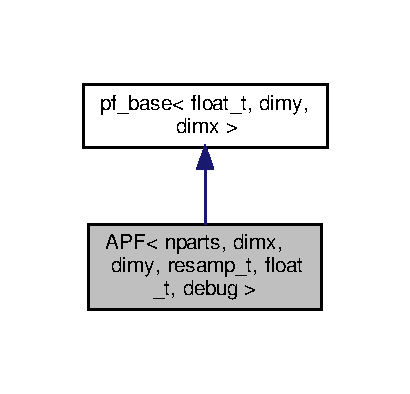
\includegraphics[width=209pt]{classAPF__inherit__graph}
\end{center}
\end{figure}


Collaboration diagram for A\+PF$<$ nparts, dimx, dimy, resamp\+\_\+t, float\+\_\+t $>$\+:\nopagebreak
\begin{figure}[H]
\begin{center}
\leavevmode
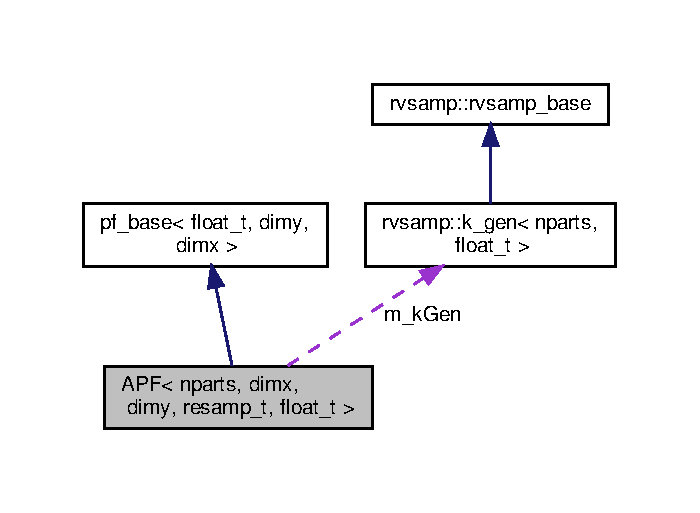
\includegraphics[width=336pt]{classAPF__coll__graph}
\end{center}
\end{figure}
\subsection*{Public Types}
\begin{DoxyCompactItemize}
\item 
using \hyperlink{classAPF_a5f96da87f00ff75af1232f9021daf06a}{ssv} = Eigen\+::\+Matrix$<$ float\+\_\+t, dimx, 1 $>$
\item 
using \hyperlink{classAPF_aa8ac25c475e54ddf21999f28727a049e}{osv} = Eigen\+::\+Matrix$<$ float\+\_\+t, dimy, 1 $>$
\item 
using \hyperlink{classAPF_a448066ff44c8afb24c89bcea11d604c6}{Mat} = Eigen\+::\+Matrix$<$ float\+\_\+t, Eigen\+::\+Dynamic, Eigen\+::\+Dynamic $>$
\item 
using \hyperlink{classAPF_ac686d94dd5c9f06febed3508dad43520}{arrayfloat\+\_\+t} = std\+::array$<$ float\+\_\+t, nparts $>$
\item 
using \hyperlink{classAPF_af0e0643ea340705993c12b1aa7ad0f4d}{array\+Vec} = std\+::array$<$ \hyperlink{classAPF_a5f96da87f00ff75af1232f9021daf06a}{ssv}, nparts $>$
\item 
using \hyperlink{classAPF_a18fed7b33bf9dbb0e3a78b87d1e75272}{array\+U\+Int} = std\+::array$<$ unsigned int, nparts $>$
\end{DoxyCompactItemize}
\subsection*{Public Member Functions}
\begin{DoxyCompactItemize}
\item 
\hyperlink{classAPF_af11ebba0fda9017d21f5d88521584210}{A\+PF} (const unsigned int \&rs=1)
\begin{DoxyCompactList}\small\item\em The constructor. \end{DoxyCompactList}\item 
\mbox{\Hypertarget{classAPF_a5f7a82bbf9d74f93c3d6ebea5f5bf95f}\label{classAPF_a5f7a82bbf9d74f93c3d6ebea5f5bf95f}} 
virtual \hyperlink{classAPF_a5f7a82bbf9d74f93c3d6ebea5f5bf95f}{$\sim$\+A\+PF} ()
\begin{DoxyCompactList}\small\item\em The (virtual) destructor. \end{DoxyCompactList}\item 
float\+\_\+t \hyperlink{classAPF_adc35c009dcf5b3289a4d46279527e024}{get\+Log\+Cond\+Like} () const
\begin{DoxyCompactList}\small\item\em Get the latest log conditional likelihood. \end{DoxyCompactList}\item 
std\+::vector$<$ \hyperlink{classAPF_a448066ff44c8afb24c89bcea11d604c6}{Mat} $>$ \hyperlink{classAPF_a5185ce1aa918dcf176bd0a3ecf6b03dd}{get\+Expectations} () const
\begin{DoxyCompactList}\small\item\em return all stored expectations (taken with respect to \$p(x\+\_\+t$\vert$y\+\_\+\{1\+:t\})\$ \end{DoxyCompactList}\item 
void \hyperlink{classAPF_ab97631b9df8b63e830070604e6887b42}{filter} (const \hyperlink{classAPF_aa8ac25c475e54ddf21999f28727a049e}{osv} \&data, const std\+::vector$<$ std\+::function$<$ const \hyperlink{classAPF_a448066ff44c8afb24c89bcea11d604c6}{Mat}(const \hyperlink{classAPF_a5f96da87f00ff75af1232f9021daf06a}{ssv} \&)$>$ $>$ \&fs=std\+::vector$<$ std\+::function$<$ const \hyperlink{classAPF_a448066ff44c8afb24c89bcea11d604c6}{Mat}(const \hyperlink{classAPF_a5f96da87f00ff75af1232f9021daf06a}{ssv} \&)$>$ $>$())
\begin{DoxyCompactList}\small\item\em Use a new datapoint to update the filtering distribution (or smoothing if path\+Length $>$ 0). \end{DoxyCompactList}\item 
virtual float\+\_\+t \hyperlink{classAPF_a7f595770b8f17cbad8e00b98e1b3bd04}{log\+Mu\+Ev} (const \hyperlink{classAPF_a5f96da87f00ff75af1232f9021daf06a}{ssv} \&x1)=0
\begin{DoxyCompactList}\small\item\em Evaluates the log of mu. \end{DoxyCompactList}\item 
virtual \hyperlink{classAPF_a5f96da87f00ff75af1232f9021daf06a}{ssv} \hyperlink{classAPF_ab57f2f5fb1af1ef6f82fbe1ca3d20905}{prop\+Mu} (const \hyperlink{classAPF_a5f96da87f00ff75af1232f9021daf06a}{ssv} \&xtm1)=0
\begin{DoxyCompactList}\small\item\em Evaluates the proposal distribution taking a Eigen\+::\+Matrix$<$float\+\_\+t,dimx,1$>$ from the previous time\textquotesingle{}s state, and returning a state for the current time. \end{DoxyCompactList}\item 
virtual \hyperlink{classAPF_a5f96da87f00ff75af1232f9021daf06a}{ssv} \hyperlink{classAPF_ad4eaf5c7d00ef9c8b8529e08bda21f13}{q1\+Samp} (const \hyperlink{classAPF_aa8ac25c475e54ddf21999f28727a049e}{osv} \&y1)=0
\begin{DoxyCompactList}\small\item\em Samples from q1. \end{DoxyCompactList}\item 
virtual \hyperlink{classAPF_a5f96da87f00ff75af1232f9021daf06a}{ssv} \hyperlink{classAPF_a30fc3aa6c6217bd4a40f07ee5a9d60d2}{f\+Samp} (const \hyperlink{classAPF_a5f96da87f00ff75af1232f9021daf06a}{ssv} \&xtm1)=0
\begin{DoxyCompactList}\small\item\em Samples from f. \end{DoxyCompactList}\item 
virtual float\+\_\+t \hyperlink{classAPF_aa892fcb9a774cd2158d107cb64f4db49}{log\+Q1\+Ev} (const \hyperlink{classAPF_a5f96da87f00ff75af1232f9021daf06a}{ssv} \&x1, const \hyperlink{classAPF_aa8ac25c475e54ddf21999f28727a049e}{osv} \&y1)=0
\begin{DoxyCompactList}\small\item\em Evaluates the log of q1. \end{DoxyCompactList}\item 
virtual float\+\_\+t \hyperlink{classAPF_ab81a714dacc1ee5ea1aa66ffee46f832}{log\+G\+Ev} (const \hyperlink{classAPF_aa8ac25c475e54ddf21999f28727a049e}{osv} \&yt, const \hyperlink{classAPF_a5f96da87f00ff75af1232f9021daf06a}{ssv} \&xt)=0
\begin{DoxyCompactList}\small\item\em Evaluates the log of g. \end{DoxyCompactList}\end{DoxyCompactItemize}
\subsection*{Protected Attributes}
\begin{DoxyCompactItemize}
\item 
\mbox{\Hypertarget{classAPF_ab1af862a00bf3d1b782b52c8996bf83f}\label{classAPF_ab1af862a00bf3d1b782b52c8996bf83f}} 
std\+::array$<$ \hyperlink{classAPF_a5f96da87f00ff75af1232f9021daf06a}{ssv}, nparts $>$ \hyperlink{classAPF_ab1af862a00bf3d1b782b52c8996bf83f}{m\+\_\+particles}
\begin{DoxyCompactList}\small\item\em particle samples \end{DoxyCompactList}\item 
\mbox{\Hypertarget{classAPF_a23f21a7901654d04256d5aa316afc386}\label{classAPF_a23f21a7901654d04256d5aa316afc386}} 
std\+::array$<$ float\+\_\+t, nparts $>$ \hyperlink{classAPF_a23f21a7901654d04256d5aa316afc386}{m\+\_\+log\+Un\+Norm\+Weights}
\begin{DoxyCompactList}\small\item\em particle unnormalized weights \end{DoxyCompactList}\item 
\mbox{\Hypertarget{classAPF_a531ab23480d146ef4b15b0cd1991e609}\label{classAPF_a531ab23480d146ef4b15b0cd1991e609}} 
unsigned int \hyperlink{classAPF_a531ab23480d146ef4b15b0cd1991e609}{m\+\_\+now}
\begin{DoxyCompactList}\small\item\em curren time \end{DoxyCompactList}\item 
\mbox{\Hypertarget{classAPF_a80465854e52cb31c53fa68bf66aad210}\label{classAPF_a80465854e52cb31c53fa68bf66aad210}} 
float\+\_\+t \hyperlink{classAPF_a80465854e52cb31c53fa68bf66aad210}{m\+\_\+log\+Last\+Cond\+Like}
\begin{DoxyCompactList}\small\item\em log p(y\+\_\+t$\vert$y\+\_\+\{1\+:t-\/1\}) or log p(y1) \end{DoxyCompactList}\item 
\mbox{\Hypertarget{classAPF_a2969bd3bee4467a47324862fefdfc693}\label{classAPF_a2969bd3bee4467a47324862fefdfc693}} 
unsigned int \hyperlink{classAPF_a2969bd3bee4467a47324862fefdfc693}{m\+\_\+rs}
\begin{DoxyCompactList}\small\item\em the resampling schedule \end{DoxyCompactList}\item 
\mbox{\Hypertarget{classAPF_aa4a7b57b66ab249a44d14ea62cb505e3}\label{classAPF_aa4a7b57b66ab249a44d14ea62cb505e3}} 
resamp\+\_\+t \hyperlink{classAPF_aa4a7b57b66ab249a44d14ea62cb505e3}{m\+\_\+resampler}
\begin{DoxyCompactList}\small\item\em resampler object (default ctor\textquotesingle{}d) \end{DoxyCompactList}\item 
\mbox{\Hypertarget{classAPF_a3288299e2f89fafd6b3dae4fbb31a887}\label{classAPF_a3288299e2f89fafd6b3dae4fbb31a887}} 
\hyperlink{classrvsamp_1_1k__gen}{rvsamp\+::k\+\_\+gen}$<$ nparts, float\+\_\+t $>$ \hyperlink{classAPF_a3288299e2f89fafd6b3dae4fbb31a887}{m\+\_\+k\+Gen}
\begin{DoxyCompactList}\small\item\em k generator object (default ctor\textquotesingle{}d) \end{DoxyCompactList}\item 
\mbox{\Hypertarget{classAPF_acd6946024490dc609f39fe4f183513df}\label{classAPF_acd6946024490dc609f39fe4f183513df}} 
std\+::vector$<$ \hyperlink{classAPF_a448066ff44c8afb24c89bcea11d604c6}{Mat} $>$ \hyperlink{classAPF_acd6946024490dc609f39fe4f183513df}{m\+\_\+expectations}
\begin{DoxyCompactList}\small\item\em expectations E\mbox{[}h(x\+\_\+t) $\vert$ y\+\_\+\{1\+:t\}\mbox{]} for user defined \char`\"{}h\char`\"{}s \end{DoxyCompactList}\end{DoxyCompactItemize}


\subsection{Detailed Description}
\subsubsection*{template$<$size\+\_\+t nparts, size\+\_\+t dimx, size\+\_\+t dimy, typename resamp\+\_\+t, typename float\+\_\+t$>$\newline
class A\+P\+F$<$ nparts, dimx, dimy, resamp\+\_\+t, float\+\_\+t $>$}

A base-\/class for Auxiliary Particle Filtering. Filtering only, no smoothing. 

\begin{DoxyAuthor}{Author}
taylor 
\end{DoxyAuthor}


\subsection{Member Typedef Documentation}
\mbox{\Hypertarget{classAPF_ac686d94dd5c9f06febed3508dad43520}\label{classAPF_ac686d94dd5c9f06febed3508dad43520}} 
\index{A\+PF@{A\+PF}!arrayfloat\+\_\+t@{arrayfloat\+\_\+t}}
\index{arrayfloat\+\_\+t@{arrayfloat\+\_\+t}!A\+PF@{A\+PF}}
\subsubsection{\texorpdfstring{arrayfloat\+\_\+t}{arrayfloat\_t}}
{\footnotesize\ttfamily template$<$size\+\_\+t nparts, size\+\_\+t dimx, size\+\_\+t dimy, typename resamp\+\_\+t , typename float\+\_\+t $>$ \\
using \hyperlink{classAPF}{A\+PF}$<$ nparts, dimx, dimy, resamp\+\_\+t, float\+\_\+t $>$\+::\hyperlink{classAPF_ac686d94dd5c9f06febed3508dad43520}{arrayfloat\+\_\+t} =  std\+::array$<$float\+\_\+t, nparts$>$}

type alias for array of float\+\_\+ts \mbox{\Hypertarget{classAPF_a18fed7b33bf9dbb0e3a78b87d1e75272}\label{classAPF_a18fed7b33bf9dbb0e3a78b87d1e75272}} 
\index{A\+PF@{A\+PF}!array\+U\+Int@{array\+U\+Int}}
\index{array\+U\+Int@{array\+U\+Int}!A\+PF@{A\+PF}}
\subsubsection{\texorpdfstring{array\+U\+Int}{arrayUInt}}
{\footnotesize\ttfamily template$<$size\+\_\+t nparts, size\+\_\+t dimx, size\+\_\+t dimy, typename resamp\+\_\+t , typename float\+\_\+t $>$ \\
using \hyperlink{classAPF}{A\+PF}$<$ nparts, dimx, dimy, resamp\+\_\+t, float\+\_\+t $>$\+::\hyperlink{classAPF_a18fed7b33bf9dbb0e3a78b87d1e75272}{array\+U\+Int} =  std\+::array$<$unsigned int, nparts$>$}

type alias for array of unsigned ints \mbox{\Hypertarget{classAPF_af0e0643ea340705993c12b1aa7ad0f4d}\label{classAPF_af0e0643ea340705993c12b1aa7ad0f4d}} 
\index{A\+PF@{A\+PF}!array\+Vec@{array\+Vec}}
\index{array\+Vec@{array\+Vec}!A\+PF@{A\+PF}}
\subsubsection{\texorpdfstring{array\+Vec}{arrayVec}}
{\footnotesize\ttfamily template$<$size\+\_\+t nparts, size\+\_\+t dimx, size\+\_\+t dimy, typename resamp\+\_\+t , typename float\+\_\+t $>$ \\
using \hyperlink{classAPF}{A\+PF}$<$ nparts, dimx, dimy, resamp\+\_\+t, float\+\_\+t $>$\+::\hyperlink{classAPF_af0e0643ea340705993c12b1aa7ad0f4d}{array\+Vec} =  std\+::array$<$\hyperlink{classAPF_a5f96da87f00ff75af1232f9021daf06a}{ssv}, nparts$>$}

type alias for array of state vectors \mbox{\Hypertarget{classAPF_a448066ff44c8afb24c89bcea11d604c6}\label{classAPF_a448066ff44c8afb24c89bcea11d604c6}} 
\index{A\+PF@{A\+PF}!Mat@{Mat}}
\index{Mat@{Mat}!A\+PF@{A\+PF}}
\subsubsection{\texorpdfstring{Mat}{Mat}}
{\footnotesize\ttfamily template$<$size\+\_\+t nparts, size\+\_\+t dimx, size\+\_\+t dimy, typename resamp\+\_\+t , typename float\+\_\+t $>$ \\
using \hyperlink{classAPF}{A\+PF}$<$ nparts, dimx, dimy, resamp\+\_\+t, float\+\_\+t $>$\+::\hyperlink{classAPF_a448066ff44c8afb24c89bcea11d604c6}{Mat} =  Eigen\+::\+Matrix$<$float\+\_\+t,Eigen\+::\+Dynamic,Eigen\+::\+Dynamic$>$}

type alias for linear algebra stuff (dimension of the state $^\wedge$2) \mbox{\Hypertarget{classAPF_aa8ac25c475e54ddf21999f28727a049e}\label{classAPF_aa8ac25c475e54ddf21999f28727a049e}} 
\index{A\+PF@{A\+PF}!osv@{osv}}
\index{osv@{osv}!A\+PF@{A\+PF}}
\subsubsection{\texorpdfstring{osv}{osv}}
{\footnotesize\ttfamily template$<$size\+\_\+t nparts, size\+\_\+t dimx, size\+\_\+t dimy, typename resamp\+\_\+t , typename float\+\_\+t $>$ \\
using \hyperlink{classAPF}{A\+PF}$<$ nparts, dimx, dimy, resamp\+\_\+t, float\+\_\+t $>$\+::\hyperlink{classAPF_aa8ac25c475e54ddf21999f28727a049e}{osv} =  Eigen\+::\+Matrix$<$float\+\_\+t,dimy,1$>$}

\char`\"{}observation size vector\char`\"{} type alias for linear algebra stuff \mbox{\Hypertarget{classAPF_a5f96da87f00ff75af1232f9021daf06a}\label{classAPF_a5f96da87f00ff75af1232f9021daf06a}} 
\index{A\+PF@{A\+PF}!ssv@{ssv}}
\index{ssv@{ssv}!A\+PF@{A\+PF}}
\subsubsection{\texorpdfstring{ssv}{ssv}}
{\footnotesize\ttfamily template$<$size\+\_\+t nparts, size\+\_\+t dimx, size\+\_\+t dimy, typename resamp\+\_\+t , typename float\+\_\+t $>$ \\
using \hyperlink{classAPF}{A\+PF}$<$ nparts, dimx, dimy, resamp\+\_\+t, float\+\_\+t $>$\+::\hyperlink{classAPF_a5f96da87f00ff75af1232f9021daf06a}{ssv} =  Eigen\+::\+Matrix$<$float\+\_\+t,dimx,1$>$}

\char`\"{}state size vector\char`\"{} type alias for linear algebra stuff 

\subsection{Constructor \& Destructor Documentation}
\mbox{\Hypertarget{classAPF_af11ebba0fda9017d21f5d88521584210}\label{classAPF_af11ebba0fda9017d21f5d88521584210}} 
\index{A\+PF@{A\+PF}!A\+PF@{A\+PF}}
\index{A\+PF@{A\+PF}!A\+PF@{A\+PF}}
\subsubsection{\texorpdfstring{A\+P\+F()}{APF()}}
{\footnotesize\ttfamily template$<$size\+\_\+t nparts, size\+\_\+t dimx, size\+\_\+t dimy, typename resamp\+\_\+t , typename float\+\_\+t $>$ \\
\hyperlink{classAPF}{A\+PF}$<$ nparts, dimx, dimy, resamp\+\_\+t, float\+\_\+t $>$\+::\hyperlink{classAPF}{A\+PF} (\begin{DoxyParamCaption}\item[{const unsigned int \&}]{rs = {\ttfamily 1} }\end{DoxyParamCaption})}



The constructor. 


\begin{DoxyParams}{Parameters}
{\em rs} & resampling schedule (e.\+g. resample every rs time points). \\
\hline
\end{DoxyParams}


\subsection{Member Function Documentation}
\mbox{\Hypertarget{classAPF_ab97631b9df8b63e830070604e6887b42}\label{classAPF_ab97631b9df8b63e830070604e6887b42}} 
\index{A\+PF@{A\+PF}!filter@{filter}}
\index{filter@{filter}!A\+PF@{A\+PF}}
\subsubsection{\texorpdfstring{filter()}{filter()}}
{\footnotesize\ttfamily template$<$size\+\_\+t nparts, size\+\_\+t dimx, size\+\_\+t dimy, typename resamp\+\_\+t , typename float\+\_\+t $>$ \\
void \hyperlink{classAPF}{A\+PF}$<$ nparts, dimx, dimy, resamp\+\_\+t, float\+\_\+t $>$\+::filter (\begin{DoxyParamCaption}\item[{const \hyperlink{classAPF_aa8ac25c475e54ddf21999f28727a049e}{osv} \&}]{data,  }\item[{const std\+::vector$<$ std\+::function$<$ const \hyperlink{classAPF_a448066ff44c8afb24c89bcea11d604c6}{Mat}(const \hyperlink{classAPF_a5f96da87f00ff75af1232f9021daf06a}{ssv} \&)$>$ $>$ \&}]{fs = {\ttfamily std\+:\+:vector$<$std\+:\+:function$<$const~\hyperlink{classAPF_a448066ff44c8afb24c89bcea11d604c6}{Mat}(const~\hyperlink{classAPF_a5f96da87f00ff75af1232f9021daf06a}{ssv}\&)$>$~$>$()} }\end{DoxyParamCaption})}



Use a new datapoint to update the filtering distribution (or smoothing if path\+Length $>$ 0). 


\begin{DoxyParams}{Parameters}
{\em data} & a Eigen\+::\+Matrix$<$float\+\_\+t,dimy,1$>$ representing the data \\
\hline
{\em fs} & a std\+::vector of callback functions that are used to calculate expectations with respect to the filtering distribution. \\
\hline
\end{DoxyParams}
\mbox{\Hypertarget{classAPF_a30fc3aa6c6217bd4a40f07ee5a9d60d2}\label{classAPF_a30fc3aa6c6217bd4a40f07ee5a9d60d2}} 
\index{A\+PF@{A\+PF}!f\+Samp@{f\+Samp}}
\index{f\+Samp@{f\+Samp}!A\+PF@{A\+PF}}
\subsubsection{\texorpdfstring{f\+Samp()}{fSamp()}}
{\footnotesize\ttfamily template$<$size\+\_\+t nparts, size\+\_\+t dimx, size\+\_\+t dimy, typename resamp\+\_\+t , typename float\+\_\+t $>$ \\
virtual \hyperlink{classAPF_a5f96da87f00ff75af1232f9021daf06a}{ssv} \hyperlink{classAPF}{A\+PF}$<$ nparts, dimx, dimy, resamp\+\_\+t, float\+\_\+t $>$\+::f\+Samp (\begin{DoxyParamCaption}\item[{const \hyperlink{classAPF_a5f96da87f00ff75af1232f9021daf06a}{ssv} \&}]{xtm1 }\end{DoxyParamCaption})\hspace{0.3cm}{\ttfamily [pure virtual]}}



Samples from f. 


\begin{DoxyParams}{Parameters}
{\em xtm1} & a Eigen\+::\+Matrix$<$float\+\_\+t,dimx,1$>$ representing the previous time\textquotesingle{}s state. \\
\hline
\end{DoxyParams}
\begin{DoxyReturn}{Returns}
a Eigen\+::\+Matrix$<$float\+\_\+t,dimx,1$>$ state sample for the current time. 
\end{DoxyReturn}
\mbox{\Hypertarget{classAPF_a5185ce1aa918dcf176bd0a3ecf6b03dd}\label{classAPF_a5185ce1aa918dcf176bd0a3ecf6b03dd}} 
\index{A\+PF@{A\+PF}!get\+Expectations@{get\+Expectations}}
\index{get\+Expectations@{get\+Expectations}!A\+PF@{A\+PF}}
\subsubsection{\texorpdfstring{get\+Expectations()}{getExpectations()}}
{\footnotesize\ttfamily template$<$size\+\_\+t nparts, size\+\_\+t dimx, size\+\_\+t dimy, typename resamp\+\_\+t , typename float\+\_\+t $>$ \\
auto \hyperlink{classAPF}{A\+PF}$<$ nparts, dimx, dimy, resamp\+\_\+t, float\+\_\+t $>$\+::get\+Expectations (\begin{DoxyParamCaption}{ }\end{DoxyParamCaption}) const}



return all stored expectations (taken with respect to \$p(x\+\_\+t$\vert$y\+\_\+\{1\+:t\})\$ 

\begin{DoxyReturn}{Returns}
return a std\+::vector$<$\+Mat$>$ of expectations. How many depends on how many callbacks you gave to 
\end{DoxyReturn}
\mbox{\Hypertarget{classAPF_adc35c009dcf5b3289a4d46279527e024}\label{classAPF_adc35c009dcf5b3289a4d46279527e024}} 
\index{A\+PF@{A\+PF}!get\+Log\+Cond\+Like@{get\+Log\+Cond\+Like}}
\index{get\+Log\+Cond\+Like@{get\+Log\+Cond\+Like}!A\+PF@{A\+PF}}
\subsubsection{\texorpdfstring{get\+Log\+Cond\+Like()}{getLogCondLike()}}
{\footnotesize\ttfamily template$<$size\+\_\+t nparts, size\+\_\+t dimx, size\+\_\+t dimy, typename resamp\+\_\+t , typename float\+\_\+t $>$ \\
float\+\_\+t \hyperlink{classAPF}{A\+PF}$<$ nparts, dimx, dimy, resamp\+\_\+t, float\+\_\+t $>$\+::get\+Log\+Cond\+Like (\begin{DoxyParamCaption}{ }\end{DoxyParamCaption}) const\hspace{0.3cm}{\ttfamily [virtual]}}



Get the latest log conditional likelihood. 

\begin{DoxyReturn}{Returns}
a float\+\_\+t of the most recent conditional likelihood. 
\end{DoxyReturn}


Implements \hyperlink{classpf__base_a350df818820d6ab0fd6d413022b7f23b}{pf\+\_\+base$<$ float\+\_\+t, dimy, dimx $>$}.

\mbox{\Hypertarget{classAPF_ab81a714dacc1ee5ea1aa66ffee46f832}\label{classAPF_ab81a714dacc1ee5ea1aa66ffee46f832}} 
\index{A\+PF@{A\+PF}!log\+G\+Ev@{log\+G\+Ev}}
\index{log\+G\+Ev@{log\+G\+Ev}!A\+PF@{A\+PF}}
\subsubsection{\texorpdfstring{log\+G\+Ev()}{logGEv()}}
{\footnotesize\ttfamily template$<$size\+\_\+t nparts, size\+\_\+t dimx, size\+\_\+t dimy, typename resamp\+\_\+t , typename float\+\_\+t $>$ \\
virtual float\+\_\+t \hyperlink{classAPF}{A\+PF}$<$ nparts, dimx, dimy, resamp\+\_\+t, float\+\_\+t $>$\+::log\+G\+Ev (\begin{DoxyParamCaption}\item[{const \hyperlink{classAPF_aa8ac25c475e54ddf21999f28727a049e}{osv} \&}]{yt,  }\item[{const \hyperlink{classAPF_a5f96da87f00ff75af1232f9021daf06a}{ssv} \&}]{xt }\end{DoxyParamCaption})\hspace{0.3cm}{\ttfamily [pure virtual]}}



Evaluates the log of g. 


\begin{DoxyParams}{Parameters}
{\em yt} & a Eigen\+::\+Matrix$<$float\+\_\+t,dimy,1$>$ representing time t\textquotesingle{}s data observation. \\
\hline
{\em xt} & a Eigen\+::\+Matrix$<$float\+\_\+t,dimx,1$>$ representing time t\textquotesingle{}s state. \\
\hline
\end{DoxyParams}
\begin{DoxyReturn}{Returns}
a float\+\_\+t evaluation. 
\end{DoxyReturn}
\mbox{\Hypertarget{classAPF_a7f595770b8f17cbad8e00b98e1b3bd04}\label{classAPF_a7f595770b8f17cbad8e00b98e1b3bd04}} 
\index{A\+PF@{A\+PF}!log\+Mu\+Ev@{log\+Mu\+Ev}}
\index{log\+Mu\+Ev@{log\+Mu\+Ev}!A\+PF@{A\+PF}}
\subsubsection{\texorpdfstring{log\+Mu\+Ev()}{logMuEv()}}
{\footnotesize\ttfamily template$<$size\+\_\+t nparts, size\+\_\+t dimx, size\+\_\+t dimy, typename resamp\+\_\+t , typename float\+\_\+t $>$ \\
virtual float\+\_\+t \hyperlink{classAPF}{A\+PF}$<$ nparts, dimx, dimy, resamp\+\_\+t, float\+\_\+t $>$\+::log\+Mu\+Ev (\begin{DoxyParamCaption}\item[{const \hyperlink{classAPF_a5f96da87f00ff75af1232f9021daf06a}{ssv} \&}]{x1 }\end{DoxyParamCaption})\hspace{0.3cm}{\ttfamily [pure virtual]}}



Evaluates the log of mu. 


\begin{DoxyParams}{Parameters}
{\em x1} & a Eigen\+::\+Matrix$<$float\+\_\+t,dimx,1$>$ representing time 1\textquotesingle{}s state. \\
\hline
\end{DoxyParams}
\begin{DoxyReturn}{Returns}
a float\+\_\+t evaluation. 
\end{DoxyReturn}
\mbox{\Hypertarget{classAPF_aa892fcb9a774cd2158d107cb64f4db49}\label{classAPF_aa892fcb9a774cd2158d107cb64f4db49}} 
\index{A\+PF@{A\+PF}!log\+Q1\+Ev@{log\+Q1\+Ev}}
\index{log\+Q1\+Ev@{log\+Q1\+Ev}!A\+PF@{A\+PF}}
\subsubsection{\texorpdfstring{log\+Q1\+Ev()}{logQ1Ev()}}
{\footnotesize\ttfamily template$<$size\+\_\+t nparts, size\+\_\+t dimx, size\+\_\+t dimy, typename resamp\+\_\+t , typename float\+\_\+t $>$ \\
virtual float\+\_\+t \hyperlink{classAPF}{A\+PF}$<$ nparts, dimx, dimy, resamp\+\_\+t, float\+\_\+t $>$\+::log\+Q1\+Ev (\begin{DoxyParamCaption}\item[{const \hyperlink{classAPF_a5f96da87f00ff75af1232f9021daf06a}{ssv} \&}]{x1,  }\item[{const \hyperlink{classAPF_aa8ac25c475e54ddf21999f28727a049e}{osv} \&}]{y1 }\end{DoxyParamCaption})\hspace{0.3cm}{\ttfamily [pure virtual]}}



Evaluates the log of q1. 


\begin{DoxyParams}{Parameters}
{\em x1} & a Eigen\+::\+Matrix$<$float\+\_\+t,dimx,1$>$ representing time 1\textquotesingle{}s state. \\
\hline
{\em y1} & a Eigen\+::\+Matrix$<$float\+\_\+t,dimy,1$>$ representing time 1\textquotesingle{}s data observation. \\
\hline
\end{DoxyParams}
\begin{DoxyReturn}{Returns}
a float\+\_\+t evaluation. 
\end{DoxyReturn}
\mbox{\Hypertarget{classAPF_ab57f2f5fb1af1ef6f82fbe1ca3d20905}\label{classAPF_ab57f2f5fb1af1ef6f82fbe1ca3d20905}} 
\index{A\+PF@{A\+PF}!prop\+Mu@{prop\+Mu}}
\index{prop\+Mu@{prop\+Mu}!A\+PF@{A\+PF}}
\subsubsection{\texorpdfstring{prop\+Mu()}{propMu()}}
{\footnotesize\ttfamily template$<$size\+\_\+t nparts, size\+\_\+t dimx, size\+\_\+t dimy, typename resamp\+\_\+t , typename float\+\_\+t $>$ \\
virtual \hyperlink{classAPF_a5f96da87f00ff75af1232f9021daf06a}{ssv} \hyperlink{classAPF}{A\+PF}$<$ nparts, dimx, dimy, resamp\+\_\+t, float\+\_\+t $>$\+::prop\+Mu (\begin{DoxyParamCaption}\item[{const \hyperlink{classAPF_a5f96da87f00ff75af1232f9021daf06a}{ssv} \&}]{xtm1 }\end{DoxyParamCaption})\hspace{0.3cm}{\ttfamily [pure virtual]}}



Evaluates the proposal distribution taking a Eigen\+::\+Matrix$<$float\+\_\+t,dimx,1$>$ from the previous time\textquotesingle{}s state, and returning a state for the current time. 


\begin{DoxyParams}{Parameters}
{\em xtm1} & a Eigen\+::\+Matrix$<$float\+\_\+t,dimx,1$>$ representing the previous time\textquotesingle{}s state. \\
\hline
\end{DoxyParams}
\begin{DoxyReturn}{Returns}
a Eigen\+::\+Matrix$<$float\+\_\+t,dimx,1$>$ representing a likely current time state, to be used by the observation density. 
\end{DoxyReturn}
\mbox{\Hypertarget{classAPF_ad4eaf5c7d00ef9c8b8529e08bda21f13}\label{classAPF_ad4eaf5c7d00ef9c8b8529e08bda21f13}} 
\index{A\+PF@{A\+PF}!q1\+Samp@{q1\+Samp}}
\index{q1\+Samp@{q1\+Samp}!A\+PF@{A\+PF}}
\subsubsection{\texorpdfstring{q1\+Samp()}{q1Samp()}}
{\footnotesize\ttfamily template$<$size\+\_\+t nparts, size\+\_\+t dimx, size\+\_\+t dimy, typename resamp\+\_\+t , typename float\+\_\+t $>$ \\
virtual \hyperlink{classAPF_a5f96da87f00ff75af1232f9021daf06a}{ssv} \hyperlink{classAPF}{A\+PF}$<$ nparts, dimx, dimy, resamp\+\_\+t, float\+\_\+t $>$\+::q1\+Samp (\begin{DoxyParamCaption}\item[{const \hyperlink{classAPF_aa8ac25c475e54ddf21999f28727a049e}{osv} \&}]{y1 }\end{DoxyParamCaption})\hspace{0.3cm}{\ttfamily [pure virtual]}}



Samples from q1. 


\begin{DoxyParams}{Parameters}
{\em y1} & a Eigen\+::\+Matrix$<$float\+\_\+t,dimy,1$>$ representing time 1\textquotesingle{}s data point. \\
\hline
\end{DoxyParams}
\begin{DoxyReturn}{Returns}
a Eigen\+::\+Matrix$<$float\+\_\+t,dimx,1$>$ sample for time 1\textquotesingle{}s state. 
\end{DoxyReturn}


The documentation for this class was generated from the following file\+:\begin{DoxyCompactItemize}
\item 
include/\hyperlink{auxiliary__pf_8h}{auxiliary\+\_\+pf.\+h}\end{DoxyCompactItemize}

\hypertarget{classrvsamp_1_1BernSampler}{}\section{rvsamp\+:\+:Bern\+Sampler$<$ float\+\_\+t, int\+\_\+t $>$ Class Template Reference}
\label{classrvsamp_1_1BernSampler}\index{rvsamp\+::\+Bern\+Sampler$<$ float\+\_\+t, int\+\_\+t $>$@{rvsamp\+::\+Bern\+Sampler$<$ float\+\_\+t, int\+\_\+t $>$}}


A class that performs sampling from a univariate Bernoulli distribution.  




{\ttfamily \#include $<$rv\+\_\+samp.\+h$>$}



Inheritance diagram for rvsamp\+:\+:Bern\+Sampler$<$ float\+\_\+t, int\+\_\+t $>$\+:
\nopagebreak
\begin{figure}[H]
\begin{center}
\leavevmode
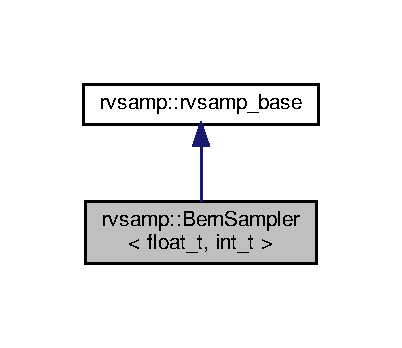
\includegraphics[width=193pt]{classrvsamp_1_1BernSampler__inherit__graph}
\end{center}
\end{figure}


Collaboration diagram for rvsamp\+:\+:Bern\+Sampler$<$ float\+\_\+t, int\+\_\+t $>$\+:
\nopagebreak
\begin{figure}[H]
\begin{center}
\leavevmode
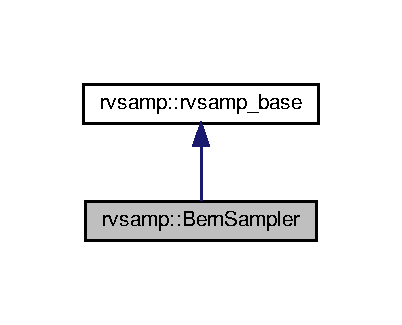
\includegraphics[width=193pt]{classrvsamp_1_1BernSampler__coll__graph}
\end{center}
\end{figure}
\subsection*{Public Member Functions}
\begin{DoxyCompactItemize}
\item 
\mbox{\Hypertarget{classrvsamp_1_1BernSampler_a85b39f1940da6d56a0d7923f684bdb5f}\label{classrvsamp_1_1BernSampler_a85b39f1940da6d56a0d7923f684bdb5f}} 
\hyperlink{classrvsamp_1_1BernSampler_a85b39f1940da6d56a0d7923f684bdb5f}{Bern\+Sampler} ()
\begin{DoxyCompactList}\small\item\em Default-\/constructor sets up for Bernoulli random variate generation with p = .5. \end{DoxyCompactList}\item 
\hyperlink{classrvsamp_1_1BernSampler_a18658e918b5bcd5cefdd900ded068686}{Bern\+Sampler} (const float\+\_\+t \&p)
\begin{DoxyCompactList}\small\item\em Constructs Bernoulli sampler with user-\/specified p. \end{DoxyCompactList}\item 
void \hyperlink{classrvsamp_1_1BernSampler_ab61c1b21be5d7422fec4ea95be91c8cc}{setP} (const float\+\_\+t \&p)
\begin{DoxyCompactList}\small\item\em sets the parameter p. \end{DoxyCompactList}\item 
int\+\_\+t \hyperlink{classrvsamp_1_1BernSampler_a2520daff5a896b58073d6756758d1323}{sample} ()
\begin{DoxyCompactList}\small\item\em Draws a random number. \end{DoxyCompactList}\end{DoxyCompactItemize}
\subsection*{Private Attributes}
\begin{DoxyCompactItemize}
\item 
\mbox{\Hypertarget{classrvsamp_1_1BernSampler_ada54494593944ed1aa4ecdafe3047e93}\label{classrvsamp_1_1BernSampler_ada54494593944ed1aa4ecdafe3047e93}} 
std\+::bernoulli\+\_\+distribution \hyperlink{classrvsamp_1_1BernSampler_ada54494593944ed1aa4ecdafe3047e93}{m\+\_\+\+B\+\_\+gen}
\begin{DoxyCompactList}\small\item\em makes normal random variates \end{DoxyCompactList}\item 
\mbox{\Hypertarget{classrvsamp_1_1BernSampler_ae0b9d07a5c37311c21c90b5d0d09ac56}\label{classrvsamp_1_1BernSampler_ae0b9d07a5c37311c21c90b5d0d09ac56}} 
float\+\_\+t \hyperlink{classrvsamp_1_1BernSampler_ae0b9d07a5c37311c21c90b5d0d09ac56}{m\+\_\+p}
\begin{DoxyCompactList}\small\item\em the mean \end{DoxyCompactList}\end{DoxyCompactItemize}
\subsection*{Additional Inherited Members}


\subsection{Detailed Description}
\subsubsection*{template$<$typename float\+\_\+t, typename int\+\_\+t$>$\newline
class rvsamp\+::\+Bern\+Sampler$<$ float\+\_\+t, int\+\_\+t $>$}

A class that performs sampling from a univariate Bernoulli distribution. 

\begin{DoxyAuthor}{Author}
taylor 
\end{DoxyAuthor}


\subsection{Constructor \& Destructor Documentation}
\mbox{\Hypertarget{classrvsamp_1_1BernSampler_a18658e918b5bcd5cefdd900ded068686}\label{classrvsamp_1_1BernSampler_a18658e918b5bcd5cefdd900ded068686}} 
\index{rvsamp\+::\+Bern\+Sampler@{rvsamp\+::\+Bern\+Sampler}!Bern\+Sampler@{Bern\+Sampler}}
\index{Bern\+Sampler@{Bern\+Sampler}!rvsamp\+::\+Bern\+Sampler@{rvsamp\+::\+Bern\+Sampler}}
\subsubsection{\texorpdfstring{Bern\+Sampler()}{BernSampler()}}
{\footnotesize\ttfamily template$<$typename float\+\_\+t , typename int\+\_\+t $>$ \\
\hyperlink{classrvsamp_1_1BernSampler}{rvsamp\+::\+Bern\+Sampler}$<$ float\+\_\+t, int\+\_\+t $>$\+::\hyperlink{classrvsamp_1_1BernSampler}{Bern\+Sampler} (\begin{DoxyParamCaption}\item[{const float\+\_\+t \&}]{p }\end{DoxyParamCaption})}



Constructs Bernoulli sampler with user-\/specified p. 


\begin{DoxyParams}{Parameters}
{\em p} & a float\+\_\+t for the probability that the rv equals 1. \\
\hline
\end{DoxyParams}


\subsection{Member Function Documentation}
\mbox{\Hypertarget{classrvsamp_1_1BernSampler_a2520daff5a896b58073d6756758d1323}\label{classrvsamp_1_1BernSampler_a2520daff5a896b58073d6756758d1323}} 
\index{rvsamp\+::\+Bern\+Sampler@{rvsamp\+::\+Bern\+Sampler}!sample@{sample}}
\index{sample@{sample}!rvsamp\+::\+Bern\+Sampler@{rvsamp\+::\+Bern\+Sampler}}
\subsubsection{\texorpdfstring{sample()}{sample()}}
{\footnotesize\ttfamily template$<$typename float\+\_\+t , typename int\+\_\+t $>$ \\
int\+\_\+t \hyperlink{classrvsamp_1_1BernSampler}{rvsamp\+::\+Bern\+Sampler}$<$ float\+\_\+t, int\+\_\+t $>$\+::sample (\begin{DoxyParamCaption}{ }\end{DoxyParamCaption})}



Draws a random number. 

\begin{DoxyReturn}{Returns}
a random sample of type float\+\_\+t. 
\end{DoxyReturn}
\mbox{\Hypertarget{classrvsamp_1_1BernSampler_ab61c1b21be5d7422fec4ea95be91c8cc}\label{classrvsamp_1_1BernSampler_ab61c1b21be5d7422fec4ea95be91c8cc}} 
\index{rvsamp\+::\+Bern\+Sampler@{rvsamp\+::\+Bern\+Sampler}!setP@{setP}}
\index{setP@{setP}!rvsamp\+::\+Bern\+Sampler@{rvsamp\+::\+Bern\+Sampler}}
\subsubsection{\texorpdfstring{set\+P()}{setP()}}
{\footnotesize\ttfamily template$<$typename float\+\_\+t , typename int\+\_\+t $>$ \\
void \hyperlink{classrvsamp_1_1BernSampler}{rvsamp\+::\+Bern\+Sampler}$<$ float\+\_\+t, int\+\_\+t $>$\+::setP (\begin{DoxyParamCaption}\item[{const float\+\_\+t \&}]{p }\end{DoxyParamCaption})}



sets the parameter p. 


\begin{DoxyParams}{Parameters}
{\em p} & the p(X=1) = 1-\/p(X=0). \\
\hline
\end{DoxyParams}


The documentation for this class was generated from the following file\+:\begin{DoxyCompactItemize}
\item 
include/\hyperlink{rv__samp_8h}{rv\+\_\+samp.\+h}\end{DoxyCompactItemize}

\hypertarget{classBSFilter}{}\section{B\+S\+Filter$<$ nparts, dimx, dimy, resamp\+\_\+t, float\+\_\+t, debug $>$ Class Template Reference}
\label{classBSFilter}\index{B\+S\+Filter$<$ nparts, dimx, dimy, resamp\+\_\+t, float\+\_\+t, debug $>$@{B\+S\+Filter$<$ nparts, dimx, dimy, resamp\+\_\+t, float\+\_\+t, debug $>$}}


A base class for the bootstrap particle filter.  




{\ttfamily \#include $<$bootstrap\+\_\+filter.\+h$>$}



Inheritance diagram for B\+S\+Filter$<$ nparts, dimx, dimy, resamp\+\_\+t, float\+\_\+t, debug $>$\+:\nopagebreak
\begin{figure}[H]
\begin{center}
\leavevmode
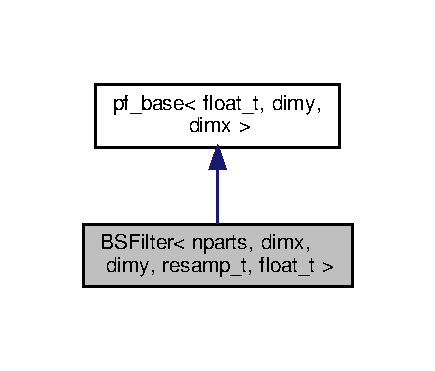
\includegraphics[width=198pt]{classBSFilter__inherit__graph}
\end{center}
\end{figure}


Collaboration diagram for B\+S\+Filter$<$ nparts, dimx, dimy, resamp\+\_\+t, float\+\_\+t, debug $>$\+:\nopagebreak
\begin{figure}[H]
\begin{center}
\leavevmode
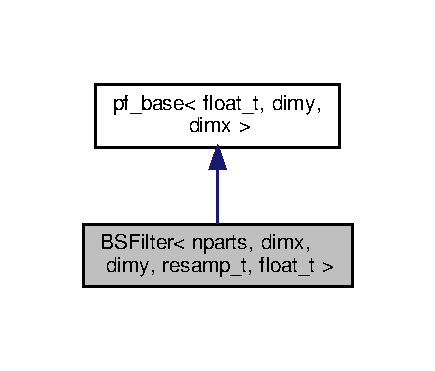
\includegraphics[width=198pt]{classBSFilter__coll__graph}
\end{center}
\end{figure}
\subsection*{Public Types}
\begin{DoxyCompactItemize}
\item 
using \hyperlink{classBSFilter_ad2341b982bcdabc798d7ed0f327d28f7}{ssv} = Eigen\+::\+Matrix$<$ float\+\_\+t, dimx, 1 $>$
\item 
using \hyperlink{classBSFilter_a9a4da560f11a6e2d35ffe693de54826b}{osv} = Eigen\+::\+Matrix$<$ float\+\_\+t, dimy, 1 $>$
\item 
using \hyperlink{classBSFilter_a190a71c131060b131c11ebe2c3fefbeb}{Mat} = Eigen\+::\+Matrix$<$ float\+\_\+t, Eigen\+::\+Dynamic, Eigen\+::\+Dynamic $>$
\item 
using \hyperlink{classBSFilter_a1d6f4a7ba66dda970cd6ea68a70fd641}{array\+States} = std\+::array$<$ \hyperlink{classBSFilter_ad2341b982bcdabc798d7ed0f327d28f7}{ssv}, nparts $>$
\item 
using \hyperlink{classBSFilter_af495dadc972ef1f8d776fe1716177aee}{array\+Float} = std\+::array$<$ float\+\_\+t, nparts $>$
\end{DoxyCompactItemize}
\subsection*{Public Member Functions}
\begin{DoxyCompactItemize}
\item 
\hyperlink{classBSFilter_ab4cab4322cfd2f3f2ed1d4d9b8d058f7}{B\+S\+Filter} (const unsigned int \&rs=1)
\begin{DoxyCompactList}\small\item\em The constructor. \end{DoxyCompactList}\item 
\mbox{\Hypertarget{classBSFilter_a73ee518e89b539464a09430ef541ea7f}\label{classBSFilter_a73ee518e89b539464a09430ef541ea7f}} 
virtual \hyperlink{classBSFilter_a73ee518e89b539464a09430ef541ea7f}{$\sim$\+B\+S\+Filter} ()
\begin{DoxyCompactList}\small\item\em The (virtual) destructor. \end{DoxyCompactList}\item 
float\+\_\+t \hyperlink{classBSFilter_a9cc91baeaaa2a22bff48d82157c86ec5}{get\+Log\+Cond\+Like} () const
\begin{DoxyCompactList}\small\item\em Returns the most recent (log-\/) conditiona likelihood. \end{DoxyCompactList}\item 
void \hyperlink{classBSFilter_a76a59b050d0cc0397b1f594a0a1c22ac}{filter} (const \hyperlink{classBSFilter_a9a4da560f11a6e2d35ffe693de54826b}{osv} \&data, const std\+::vector$<$ std\+::function$<$ const \hyperlink{classBSFilter_a190a71c131060b131c11ebe2c3fefbeb}{Mat}(const \hyperlink{classBSFilter_ad2341b982bcdabc798d7ed0f327d28f7}{ssv} \&)$>$ $>$ \&fs=std\+::vector$<$ std\+::function$<$ const \hyperlink{classBSFilter_a190a71c131060b131c11ebe2c3fefbeb}{Mat}(const \hyperlink{classBSFilter_ad2341b982bcdabc798d7ed0f327d28f7}{ssv} \&)$>$ $>$())
\begin{DoxyCompactList}\small\item\em updates filtering distribution on a new datapoint. Optionally stores expectations of functionals. \end{DoxyCompactList}\item 
auto \hyperlink{classBSFilter_a837a9dc83c07195fb96b4228dc8e41fe}{get\+Expectations} () const -\/$>$ std\+::vector$<$ \hyperlink{classBSFilter_a190a71c131060b131c11ebe2c3fefbeb}{Mat} $>$
\begin{DoxyCompactList}\small\item\em return all stored expectations (taken with respect to \$p(x\+\_\+t$\vert$y\+\_\+\{1\+:t\})\$ \end{DoxyCompactList}\item 
virtual float\+\_\+t \hyperlink{classBSFilter_a460a1a2f97a5d1088a95f6b766e9dc56}{log\+Mu\+Ev} (const \hyperlink{classBSFilter_ad2341b982bcdabc798d7ed0f327d28f7}{ssv} \&x1)=0
\begin{DoxyCompactList}\small\item\em Calculate mu\+Ev or logmu\+Ev. \end{DoxyCompactList}\item 
virtual \hyperlink{classBSFilter_ad2341b982bcdabc798d7ed0f327d28f7}{ssv} \hyperlink{classBSFilter_a82185282cbc7ddf5983933ccd7705577}{q1\+Samp} (const \hyperlink{classBSFilter_a9a4da560f11a6e2d35ffe693de54826b}{osv} \&y1)=0
\begin{DoxyCompactList}\small\item\em Samples from time 1 proposal. \end{DoxyCompactList}\item 
virtual float\+\_\+t \hyperlink{classBSFilter_a81321d8ca9960ea4102c6fe3dc7b7636}{log\+Q1\+Ev} (const \hyperlink{classBSFilter_ad2341b982bcdabc798d7ed0f327d28f7}{ssv} \&x1, const \hyperlink{classBSFilter_a9a4da560f11a6e2d35ffe693de54826b}{osv} \&y1)=0
\begin{DoxyCompactList}\small\item\em Calculate q1\+Ev or log q1\+Ev. \end{DoxyCompactList}\item 
virtual float\+\_\+t \hyperlink{classBSFilter_a1cf2ed5153756a015384d459e72a57de}{log\+G\+Ev} (const \hyperlink{classBSFilter_a9a4da560f11a6e2d35ffe693de54826b}{osv} \&yt, const \hyperlink{classBSFilter_ad2341b982bcdabc798d7ed0f327d28f7}{ssv} \&xt)=0
\begin{DoxyCompactList}\small\item\em Calculate g\+Ev or log\+G\+Ev. \end{DoxyCompactList}\item 
virtual \hyperlink{classBSFilter_ad2341b982bcdabc798d7ed0f327d28f7}{ssv} \hyperlink{classBSFilter_ac97a15ea8002b48e56d94c8de699caa2}{f\+Samp} (const \hyperlink{classBSFilter_ad2341b982bcdabc798d7ed0f327d28f7}{ssv} \&xtm1)=0
\begin{DoxyCompactList}\small\item\em Sample from the state transition distribution. \end{DoxyCompactList}\end{DoxyCompactItemize}
\subsection*{Static Public Attributes}
\begin{DoxyCompactItemize}
\item 
static constexpr unsigned int \hyperlink{classBSFilter_a2a6b1e1870c1a4f3e7ca0b721b697ce2}{num\+\_\+particles} = nparts
\end{DoxyCompactItemize}
\subsection*{Protected Attributes}
\begin{DoxyCompactItemize}
\item 
\mbox{\Hypertarget{classBSFilter_a52dde1eb7fe247f783f4f2e5388f86ac}\label{classBSFilter_a52dde1eb7fe247f783f4f2e5388f86ac}} 
\hyperlink{classBSFilter_a1d6f4a7ba66dda970cd6ea68a70fd641}{array\+States} \hyperlink{classBSFilter_a52dde1eb7fe247f783f4f2e5388f86ac}{m\+\_\+particles}
\begin{DoxyCompactList}\small\item\em particle samples \end{DoxyCompactList}\item 
\mbox{\Hypertarget{classBSFilter_a06b115e9578557bbef4064e43b1afbbe}\label{classBSFilter_a06b115e9578557bbef4064e43b1afbbe}} 
\hyperlink{classBSFilter_af495dadc972ef1f8d776fe1716177aee}{array\+Float} \hyperlink{classBSFilter_a06b115e9578557bbef4064e43b1afbbe}{m\+\_\+log\+Un\+Norm\+Weights}
\begin{DoxyCompactList}\small\item\em particle unnormalized weights \end{DoxyCompactList}\item 
\mbox{\Hypertarget{classBSFilter_adf89ebde89f4ab2d5aa7754042481345}\label{classBSFilter_adf89ebde89f4ab2d5aa7754042481345}} 
unsigned int \hyperlink{classBSFilter_adf89ebde89f4ab2d5aa7754042481345}{m\+\_\+now}
\begin{DoxyCompactList}\small\item\em time point \end{DoxyCompactList}\item 
\mbox{\Hypertarget{classBSFilter_a4aca072edced8670e55023a47ffd551a}\label{classBSFilter_a4aca072edced8670e55023a47ffd551a}} 
float\+\_\+t \hyperlink{classBSFilter_a4aca072edced8670e55023a47ffd551a}{m\+\_\+log\+Last\+Cond\+Like}
\begin{DoxyCompactList}\small\item\em log p(y\+\_\+t$\vert$y\+\_\+\{1\+:t-\/1\}) or log p(y1) \end{DoxyCompactList}\item 
\mbox{\Hypertarget{classBSFilter_aff77ccb7698f098b7d88781a20cef538}\label{classBSFilter_aff77ccb7698f098b7d88781a20cef538}} 
resamp\+\_\+t \hyperlink{classBSFilter_aff77ccb7698f098b7d88781a20cef538}{m\+\_\+resampler}
\begin{DoxyCompactList}\small\item\em resampler object \end{DoxyCompactList}\item 
\mbox{\Hypertarget{classBSFilter_ad36944944fce5d23663245c8cc0a296a}\label{classBSFilter_ad36944944fce5d23663245c8cc0a296a}} 
std\+::vector$<$ \hyperlink{classBSFilter_a190a71c131060b131c11ebe2c3fefbeb}{Mat} $>$ \hyperlink{classBSFilter_ad36944944fce5d23663245c8cc0a296a}{m\+\_\+expectations}
\begin{DoxyCompactList}\small\item\em expectations E\mbox{[}h(x\+\_\+t) $\vert$ y\+\_\+\{1\+:t\}\mbox{]} for user defined \char`\"{}h\char`\"{}s \end{DoxyCompactList}\item 
\mbox{\Hypertarget{classBSFilter_a1962760bd541b6dbea7da7c5572f60e0}\label{classBSFilter_a1962760bd541b6dbea7da7c5572f60e0}} 
unsigned int \hyperlink{classBSFilter_a1962760bd541b6dbea7da7c5572f60e0}{m\+\_\+resamp\+Sched}
\begin{DoxyCompactList}\small\item\em resampling schedule (e.\+g. resample every \+\_\+\+\_\+ time points) \end{DoxyCompactList}\end{DoxyCompactItemize}


\subsection{Detailed Description}
\subsubsection*{template$<$size\+\_\+t nparts, size\+\_\+t dimx, size\+\_\+t dimy, typename resamp\+\_\+t, typename float\+\_\+t, bool debug = false$>$\newline
class B\+S\+Filter$<$ nparts, dimx, dimy, resamp\+\_\+t, float\+\_\+t, debug $>$}

A base class for the bootstrap particle filter. 

\begin{DoxyAuthor}{Author}
taylor 
\end{DoxyAuthor}


\subsection{Member Typedef Documentation}
\mbox{\Hypertarget{classBSFilter_af495dadc972ef1f8d776fe1716177aee}\label{classBSFilter_af495dadc972ef1f8d776fe1716177aee}} 
\index{B\+S\+Filter@{B\+S\+Filter}!array\+Float@{array\+Float}}
\index{array\+Float@{array\+Float}!B\+S\+Filter@{B\+S\+Filter}}
\subsubsection{\texorpdfstring{array\+Float}{arrayFloat}}
{\footnotesize\ttfamily template$<$size\+\_\+t nparts, size\+\_\+t dimx, size\+\_\+t dimy, typename resamp\+\_\+t , typename float\+\_\+t , bool debug = false$>$ \\
using \hyperlink{classBSFilter}{B\+S\+Filter}$<$ nparts, dimx, dimy, resamp\+\_\+t, float\+\_\+t, debug $>$\+::\hyperlink{classBSFilter_af495dadc972ef1f8d776fe1716177aee}{array\+Float} =  std\+::array$<$float\+\_\+t, nparts$>$}

type alias for array of floating points \mbox{\Hypertarget{classBSFilter_a1d6f4a7ba66dda970cd6ea68a70fd641}\label{classBSFilter_a1d6f4a7ba66dda970cd6ea68a70fd641}} 
\index{B\+S\+Filter@{B\+S\+Filter}!array\+States@{array\+States}}
\index{array\+States@{array\+States}!B\+S\+Filter@{B\+S\+Filter}}
\subsubsection{\texorpdfstring{array\+States}{arrayStates}}
{\footnotesize\ttfamily template$<$size\+\_\+t nparts, size\+\_\+t dimx, size\+\_\+t dimy, typename resamp\+\_\+t , typename float\+\_\+t , bool debug = false$>$ \\
using \hyperlink{classBSFilter}{B\+S\+Filter}$<$ nparts, dimx, dimy, resamp\+\_\+t, float\+\_\+t, debug $>$\+::\hyperlink{classBSFilter_a1d6f4a7ba66dda970cd6ea68a70fd641}{array\+States} =  std\+::array$<$\hyperlink{classBSFilter_ad2341b982bcdabc798d7ed0f327d28f7}{ssv}, nparts$>$}

type alias for linear algebra stuff \mbox{\Hypertarget{classBSFilter_a190a71c131060b131c11ebe2c3fefbeb}\label{classBSFilter_a190a71c131060b131c11ebe2c3fefbeb}} 
\index{B\+S\+Filter@{B\+S\+Filter}!Mat@{Mat}}
\index{Mat@{Mat}!B\+S\+Filter@{B\+S\+Filter}}
\subsubsection{\texorpdfstring{Mat}{Mat}}
{\footnotesize\ttfamily template$<$size\+\_\+t nparts, size\+\_\+t dimx, size\+\_\+t dimy, typename resamp\+\_\+t , typename float\+\_\+t , bool debug = false$>$ \\
using \hyperlink{classBSFilter}{B\+S\+Filter}$<$ nparts, dimx, dimy, resamp\+\_\+t, float\+\_\+t, debug $>$\+::\hyperlink{classBSFilter_a190a71c131060b131c11ebe2c3fefbeb}{Mat} =  Eigen\+::\+Matrix$<$float\+\_\+t, Eigen\+::\+Dynamic, Eigen\+::\+Dynamic$>$}

type alias for dynamically sized matrix \mbox{\Hypertarget{classBSFilter_a9a4da560f11a6e2d35ffe693de54826b}\label{classBSFilter_a9a4da560f11a6e2d35ffe693de54826b}} 
\index{B\+S\+Filter@{B\+S\+Filter}!osv@{osv}}
\index{osv@{osv}!B\+S\+Filter@{B\+S\+Filter}}
\subsubsection{\texorpdfstring{osv}{osv}}
{\footnotesize\ttfamily template$<$size\+\_\+t nparts, size\+\_\+t dimx, size\+\_\+t dimy, typename resamp\+\_\+t , typename float\+\_\+t , bool debug = false$>$ \\
using \hyperlink{classBSFilter}{B\+S\+Filter}$<$ nparts, dimx, dimy, resamp\+\_\+t, float\+\_\+t, debug $>$\+::\hyperlink{classBSFilter_a9a4da560f11a6e2d35ffe693de54826b}{osv} =  Eigen\+::\+Matrix$<$float\+\_\+t, dimy, 1$>$}

\char`\"{}obs size vector\char`\"{} type alias for linear algebra stuff \mbox{\Hypertarget{classBSFilter_ad2341b982bcdabc798d7ed0f327d28f7}\label{classBSFilter_ad2341b982bcdabc798d7ed0f327d28f7}} 
\index{B\+S\+Filter@{B\+S\+Filter}!ssv@{ssv}}
\index{ssv@{ssv}!B\+S\+Filter@{B\+S\+Filter}}
\subsubsection{\texorpdfstring{ssv}{ssv}}
{\footnotesize\ttfamily template$<$size\+\_\+t nparts, size\+\_\+t dimx, size\+\_\+t dimy, typename resamp\+\_\+t , typename float\+\_\+t , bool debug = false$>$ \\
using \hyperlink{classBSFilter}{B\+S\+Filter}$<$ nparts, dimx, dimy, resamp\+\_\+t, float\+\_\+t, debug $>$\+::\hyperlink{classBSFilter_ad2341b982bcdabc798d7ed0f327d28f7}{ssv} =  Eigen\+::\+Matrix$<$float\+\_\+t, dimx, 1$>$}

\char`\"{}state size vector\char`\"{} type alias for linear algebra stuff 

\subsection{Constructor \& Destructor Documentation}
\mbox{\Hypertarget{classBSFilter_ab4cab4322cfd2f3f2ed1d4d9b8d058f7}\label{classBSFilter_ab4cab4322cfd2f3f2ed1d4d9b8d058f7}} 
\index{B\+S\+Filter@{B\+S\+Filter}!B\+S\+Filter@{B\+S\+Filter}}
\index{B\+S\+Filter@{B\+S\+Filter}!B\+S\+Filter@{B\+S\+Filter}}
\subsubsection{\texorpdfstring{B\+S\+Filter()}{BSFilter()}}
{\footnotesize\ttfamily template$<$size\+\_\+t nparts, size\+\_\+t dimx, size\+\_\+t dimy, typename resamp\+\_\+t , typename float\+\_\+t , bool debug$>$ \\
\hyperlink{classBSFilter}{B\+S\+Filter}$<$ nparts, dimx, dimy, resamp\+\_\+t, float\+\_\+t, debug $>$\+::\hyperlink{classBSFilter}{B\+S\+Filter} (\begin{DoxyParamCaption}\item[{const unsigned int \&}]{rs = {\ttfamily 1} }\end{DoxyParamCaption})}



The constructor. 


\begin{DoxyParams}{Parameters}
{\em rs} & the resampling schedule (e.\+g. every rs time point) \\
\hline
\end{DoxyParams}


\subsection{Member Function Documentation}
\mbox{\Hypertarget{classBSFilter_a76a59b050d0cc0397b1f594a0a1c22ac}\label{classBSFilter_a76a59b050d0cc0397b1f594a0a1c22ac}} 
\index{B\+S\+Filter@{B\+S\+Filter}!filter@{filter}}
\index{filter@{filter}!B\+S\+Filter@{B\+S\+Filter}}
\subsubsection{\texorpdfstring{filter()}{filter()}}
{\footnotesize\ttfamily template$<$size\+\_\+t nparts, size\+\_\+t dimx, size\+\_\+t dimy, typename resamp\+\_\+t , typename float\+\_\+t , bool debug$>$ \\
void \hyperlink{classBSFilter}{B\+S\+Filter}$<$ nparts, dimx, dimy, resamp\+\_\+t, float\+\_\+t, debug $>$\+::filter (\begin{DoxyParamCaption}\item[{const \hyperlink{classBSFilter_a9a4da560f11a6e2d35ffe693de54826b}{osv} \&}]{data,  }\item[{const std\+::vector$<$ std\+::function$<$ const \hyperlink{classBSFilter_a190a71c131060b131c11ebe2c3fefbeb}{Mat}(const \hyperlink{classBSFilter_ad2341b982bcdabc798d7ed0f327d28f7}{ssv} \&)$>$ $>$ \&}]{fs = {\ttfamily std\+:\+:vector$<$std\+:\+:function$<$const~\hyperlink{classBSFilter_a190a71c131060b131c11ebe2c3fefbeb}{Mat}(const~\hyperlink{classBSFilter_ad2341b982bcdabc798d7ed0f327d28f7}{ssv}\&)$>$~$>$()} }\end{DoxyParamCaption})}



updates filtering distribution on a new datapoint. Optionally stores expectations of functionals. 


\begin{DoxyParams}{Parameters}
{\em data} & the most recent data point \\
\hline
{\em fs} & a vector of functions if you want to calculate expectations. \\
\hline
\end{DoxyParams}
\mbox{\Hypertarget{classBSFilter_ac97a15ea8002b48e56d94c8de699caa2}\label{classBSFilter_ac97a15ea8002b48e56d94c8de699caa2}} 
\index{B\+S\+Filter@{B\+S\+Filter}!f\+Samp@{f\+Samp}}
\index{f\+Samp@{f\+Samp}!B\+S\+Filter@{B\+S\+Filter}}
\subsubsection{\texorpdfstring{f\+Samp()}{fSamp()}}
{\footnotesize\ttfamily template$<$size\+\_\+t nparts, size\+\_\+t dimx, size\+\_\+t dimy, typename resamp\+\_\+t , typename float\+\_\+t , bool debug = false$>$ \\
virtual \hyperlink{classBSFilter_ad2341b982bcdabc798d7ed0f327d28f7}{ssv} \hyperlink{classBSFilter}{B\+S\+Filter}$<$ nparts, dimx, dimy, resamp\+\_\+t, float\+\_\+t, debug $>$\+::f\+Samp (\begin{DoxyParamCaption}\item[{const \hyperlink{classBSFilter_ad2341b982bcdabc798d7ed0f327d28f7}{ssv} \&}]{xtm1 }\end{DoxyParamCaption})\hspace{0.3cm}{\ttfamily [pure virtual]}}



Sample from the state transition distribution. 


\begin{DoxyParams}{Parameters}
{\em xtm1} & is a const Vec\& describing the time t-\/1 state \\
\hline
\end{DoxyParams}
\begin{DoxyReturn}{Returns}
the sample as a Vec 
\end{DoxyReturn}
\mbox{\Hypertarget{classBSFilter_a837a9dc83c07195fb96b4228dc8e41fe}\label{classBSFilter_a837a9dc83c07195fb96b4228dc8e41fe}} 
\index{B\+S\+Filter@{B\+S\+Filter}!get\+Expectations@{get\+Expectations}}
\index{get\+Expectations@{get\+Expectations}!B\+S\+Filter@{B\+S\+Filter}}
\subsubsection{\texorpdfstring{get\+Expectations()}{getExpectations()}}
{\footnotesize\ttfamily template$<$size\+\_\+t nparts, size\+\_\+t dimx, size\+\_\+t dimy, typename resamp\+\_\+t , typename float\+\_\+t , bool debug$>$ \\
auto \hyperlink{classBSFilter}{B\+S\+Filter}$<$ nparts, dimx, dimy, resamp\+\_\+t, float\+\_\+t, debug $>$\+::get\+Expectations (\begin{DoxyParamCaption}{ }\end{DoxyParamCaption}) const -\/$>$ std\+::vector$<$\hyperlink{classBSFilter_a190a71c131060b131c11ebe2c3fefbeb}{Mat}$>$}



return all stored expectations (taken with respect to \$p(x\+\_\+t$\vert$y\+\_\+\{1\+:t\})\$ 

\begin{DoxyReturn}{Returns}
return a std\+::vector$<$\+Mat$>$ of expectations. How many depends on how many callbacks you gave to 
\end{DoxyReturn}
\mbox{\Hypertarget{classBSFilter_a9cc91baeaaa2a22bff48d82157c86ec5}\label{classBSFilter_a9cc91baeaaa2a22bff48d82157c86ec5}} 
\index{B\+S\+Filter@{B\+S\+Filter}!get\+Log\+Cond\+Like@{get\+Log\+Cond\+Like}}
\index{get\+Log\+Cond\+Like@{get\+Log\+Cond\+Like}!B\+S\+Filter@{B\+S\+Filter}}
\subsubsection{\texorpdfstring{get\+Log\+Cond\+Like()}{getLogCondLike()}}
{\footnotesize\ttfamily template$<$size\+\_\+t nparts, size\+\_\+t dimx, size\+\_\+t dimy, typename resamp\+\_\+t , typename float\+\_\+t , bool debug$>$ \\
float\+\_\+t \hyperlink{classBSFilter}{B\+S\+Filter}$<$ nparts, dimx, dimy, resamp\+\_\+t, float\+\_\+t, debug $>$\+::get\+Log\+Cond\+Like (\begin{DoxyParamCaption}{ }\end{DoxyParamCaption}) const\hspace{0.3cm}{\ttfamily [virtual]}}



Returns the most recent (log-\/) conditiona likelihood. 

\begin{DoxyReturn}{Returns}
log p(y\+\_\+t $\vert$ y\+\_\+\{1\+:t-\/1\}) 
\end{DoxyReturn}


Implements \hyperlink{classpf__base_a350df818820d6ab0fd6d413022b7f23b}{pf\+\_\+base$<$ float\+\_\+t, dimy, dimx $>$}.

\mbox{\Hypertarget{classBSFilter_a1cf2ed5153756a015384d459e72a57de}\label{classBSFilter_a1cf2ed5153756a015384d459e72a57de}} 
\index{B\+S\+Filter@{B\+S\+Filter}!log\+G\+Ev@{log\+G\+Ev}}
\index{log\+G\+Ev@{log\+G\+Ev}!B\+S\+Filter@{B\+S\+Filter}}
\subsubsection{\texorpdfstring{log\+G\+Ev()}{logGEv()}}
{\footnotesize\ttfamily template$<$size\+\_\+t nparts, size\+\_\+t dimx, size\+\_\+t dimy, typename resamp\+\_\+t , typename float\+\_\+t , bool debug = false$>$ \\
virtual float\+\_\+t \hyperlink{classBSFilter}{B\+S\+Filter}$<$ nparts, dimx, dimy, resamp\+\_\+t, float\+\_\+t, debug $>$\+::log\+G\+Ev (\begin{DoxyParamCaption}\item[{const \hyperlink{classBSFilter_a9a4da560f11a6e2d35ffe693de54826b}{osv} \&}]{yt,  }\item[{const \hyperlink{classBSFilter_ad2341b982bcdabc798d7ed0f327d28f7}{ssv} \&}]{xt }\end{DoxyParamCaption})\hspace{0.3cm}{\ttfamily [pure virtual]}}



Calculate g\+Ev or log\+G\+Ev. 


\begin{DoxyParams}{Parameters}
{\em yt} & is a const Vec\& describing the time t datum \\
\hline
{\em xt} & is a const Vec\& describing the time t state \\
\hline
\end{DoxyParams}
\begin{DoxyReturn}{Returns}
the density or log-\/density evaluation 
\end{DoxyReturn}
\mbox{\Hypertarget{classBSFilter_a460a1a2f97a5d1088a95f6b766e9dc56}\label{classBSFilter_a460a1a2f97a5d1088a95f6b766e9dc56}} 
\index{B\+S\+Filter@{B\+S\+Filter}!log\+Mu\+Ev@{log\+Mu\+Ev}}
\index{log\+Mu\+Ev@{log\+Mu\+Ev}!B\+S\+Filter@{B\+S\+Filter}}
\subsubsection{\texorpdfstring{log\+Mu\+Ev()}{logMuEv()}}
{\footnotesize\ttfamily template$<$size\+\_\+t nparts, size\+\_\+t dimx, size\+\_\+t dimy, typename resamp\+\_\+t , typename float\+\_\+t , bool debug = false$>$ \\
virtual float\+\_\+t \hyperlink{classBSFilter}{B\+S\+Filter}$<$ nparts, dimx, dimy, resamp\+\_\+t, float\+\_\+t, debug $>$\+::log\+Mu\+Ev (\begin{DoxyParamCaption}\item[{const \hyperlink{classBSFilter_ad2341b982bcdabc798d7ed0f327d28f7}{ssv} \&}]{x1 }\end{DoxyParamCaption})\hspace{0.3cm}{\ttfamily [pure virtual]}}



Calculate mu\+Ev or logmu\+Ev. 


\begin{DoxyParams}{Parameters}
{\em x1} & is a const Vec\& describing the state sample \\
\hline
\end{DoxyParams}
\begin{DoxyReturn}{Returns}
the density or log-\/density evaluation 
\end{DoxyReturn}
\mbox{\Hypertarget{classBSFilter_a81321d8ca9960ea4102c6fe3dc7b7636}\label{classBSFilter_a81321d8ca9960ea4102c6fe3dc7b7636}} 
\index{B\+S\+Filter@{B\+S\+Filter}!log\+Q1\+Ev@{log\+Q1\+Ev}}
\index{log\+Q1\+Ev@{log\+Q1\+Ev}!B\+S\+Filter@{B\+S\+Filter}}
\subsubsection{\texorpdfstring{log\+Q1\+Ev()}{logQ1Ev()}}
{\footnotesize\ttfamily template$<$size\+\_\+t nparts, size\+\_\+t dimx, size\+\_\+t dimy, typename resamp\+\_\+t , typename float\+\_\+t , bool debug = false$>$ \\
virtual float\+\_\+t \hyperlink{classBSFilter}{B\+S\+Filter}$<$ nparts, dimx, dimy, resamp\+\_\+t, float\+\_\+t, debug $>$\+::log\+Q1\+Ev (\begin{DoxyParamCaption}\item[{const \hyperlink{classBSFilter_ad2341b982bcdabc798d7ed0f327d28f7}{ssv} \&}]{x1,  }\item[{const \hyperlink{classBSFilter_a9a4da560f11a6e2d35ffe693de54826b}{osv} \&}]{y1 }\end{DoxyParamCaption})\hspace{0.3cm}{\ttfamily [pure virtual]}}



Calculate q1\+Ev or log q1\+Ev. 


\begin{DoxyParams}{Parameters}
{\em x1} & is a const Vec\& describing the time 1 state sample \\
\hline
{\em y1} & is a const Vec\& describing the time 1 datum \\
\hline
\end{DoxyParams}
\begin{DoxyReturn}{Returns}
the density or log-\/density evaluation 
\end{DoxyReturn}
\mbox{\Hypertarget{classBSFilter_a82185282cbc7ddf5983933ccd7705577}\label{classBSFilter_a82185282cbc7ddf5983933ccd7705577}} 
\index{B\+S\+Filter@{B\+S\+Filter}!q1\+Samp@{q1\+Samp}}
\index{q1\+Samp@{q1\+Samp}!B\+S\+Filter@{B\+S\+Filter}}
\subsubsection{\texorpdfstring{q1\+Samp()}{q1Samp()}}
{\footnotesize\ttfamily template$<$size\+\_\+t nparts, size\+\_\+t dimx, size\+\_\+t dimy, typename resamp\+\_\+t , typename float\+\_\+t , bool debug = false$>$ \\
virtual \hyperlink{classBSFilter_ad2341b982bcdabc798d7ed0f327d28f7}{ssv} \hyperlink{classBSFilter}{B\+S\+Filter}$<$ nparts, dimx, dimy, resamp\+\_\+t, float\+\_\+t, debug $>$\+::q1\+Samp (\begin{DoxyParamCaption}\item[{const \hyperlink{classBSFilter_a9a4da560f11a6e2d35ffe693de54826b}{osv} \&}]{y1 }\end{DoxyParamCaption})\hspace{0.3cm}{\ttfamily [pure virtual]}}



Samples from time 1 proposal. 


\begin{DoxyParams}{Parameters}
{\em y1} & is a const Vec\& representing the first observed datum \\
\hline
\end{DoxyParams}
\begin{DoxyReturn}{Returns}
the sample as a Vec 
\end{DoxyReturn}


\subsection{Member Data Documentation}
\mbox{\Hypertarget{classBSFilter_a2a6b1e1870c1a4f3e7ca0b721b697ce2}\label{classBSFilter_a2a6b1e1870c1a4f3e7ca0b721b697ce2}} 
\index{B\+S\+Filter@{B\+S\+Filter}!num\+\_\+particles@{num\+\_\+particles}}
\index{num\+\_\+particles@{num\+\_\+particles}!B\+S\+Filter@{B\+S\+Filter}}
\subsubsection{\texorpdfstring{num\+\_\+particles}{num\_particles}}
{\footnotesize\ttfamily template$<$size\+\_\+t nparts, size\+\_\+t dimx, size\+\_\+t dimy, typename resamp\+\_\+t , typename float\+\_\+t , bool debug = false$>$ \\
constexpr unsigned int \hyperlink{classBSFilter}{B\+S\+Filter}$<$ nparts, dimx, dimy, resamp\+\_\+t, float\+\_\+t, debug $>$\+::num\+\_\+particles = nparts\hspace{0.3cm}{\ttfamily [static]}}

the number of particles 

The documentation for this class was generated from the following file\+:\begin{DoxyCompactItemize}
\item 
include/pf/\hyperlink{bootstrap__filter_8h}{bootstrap\+\_\+filter.\+h}\end{DoxyCompactItemize}

\hypertarget{classBSFilterWC}{}\section{B\+S\+Filter\+WC$<$ nparts, dimx, dimy, dimcov, resamp\+\_\+t, float\+\_\+t $>$ Class Template Reference}
\label{classBSFilterWC}\index{B\+S\+Filter\+W\+C$<$ nparts, dimx, dimy, dimcov, resamp\+\_\+t, float\+\_\+t $>$@{B\+S\+Filter\+W\+C$<$ nparts, dimx, dimy, dimcov, resamp\+\_\+t, float\+\_\+t $>$}}


A base class for the bootstrap particle filter with covariates.  




{\ttfamily \#include $<$bootstrap\+\_\+filter\+\_\+with\+\_\+covariates.\+h$>$}

\subsection*{Public Types}
\begin{DoxyCompactItemize}
\item 
using \hyperlink{classBSFilterWC_afff292a8cc15505cc3aa244135203c78}{ssv} = Eigen\+::\+Matrix$<$ float\+\_\+t, dimx, 1 $>$
\item 
using \hyperlink{classBSFilterWC_a48b0c7f1a1cf7e57300cf820e74057ce}{osv} = Eigen\+::\+Matrix$<$ float\+\_\+t, dimy, 1 $>$
\item 
using \hyperlink{classBSFilterWC_a52f5a46901a821fffe82937543220a1a}{cvsv} = Eigen\+::\+Matrix$<$ float\+\_\+t, dimcov, 1 $>$
\item 
using \hyperlink{classBSFilterWC_a507a06203a27e3a025a43be68b4b0e0e}{Mat} = Eigen\+::\+Matrix$<$ float\+\_\+t, Eigen\+::\+Dynamic, Eigen\+::\+Dynamic $>$
\item 
using \hyperlink{classBSFilterWC_af89dac8c324ae8b549595a85e89ec7da}{array\+States} = std\+::array$<$ \hyperlink{classBSFilterWC_afff292a8cc15505cc3aa244135203c78}{ssv}, nparts $>$
\item 
using \hyperlink{classBSFilterWC_a12c3f32cb628a0efaa0267262205d6d6}{arrayfloat\+\_\+t} = std\+::array$<$ float\+\_\+t, nparts $>$
\item 
using \hyperlink{classBSFilterWC_a984a5a75eef118f2f4db7f8953fea653}{Funcs} = std\+::vector$<$ std\+::function$<$ const \hyperlink{classBSFilterWC_a507a06203a27e3a025a43be68b4b0e0e}{Mat}(const \hyperlink{classBSFilterWC_afff292a8cc15505cc3aa244135203c78}{ssv} \&, const \hyperlink{classBSFilterWC_a52f5a46901a821fffe82937543220a1a}{cvsv} \&)$>$ $>$
\end{DoxyCompactItemize}
\subsection*{Public Member Functions}
\begin{DoxyCompactItemize}
\item 
\hyperlink{classBSFilterWC_a8b9399d0b7008aa6bca19a87834dfd6a}{B\+S\+Filter\+WC} (const unsigned int \&rs=1)
\begin{DoxyCompactList}\small\item\em The constructor. \end{DoxyCompactList}\item 
\mbox{\Hypertarget{classBSFilterWC_a125b13d2ba71b3bce05c315dea38b476}\label{classBSFilterWC_a125b13d2ba71b3bce05c315dea38b476}} 
virtual \hyperlink{classBSFilterWC_a125b13d2ba71b3bce05c315dea38b476}{$\sim$\+B\+S\+Filter\+WC} ()
\begin{DoxyCompactList}\small\item\em The (virtual) destructor. \end{DoxyCompactList}\item 
float\+\_\+t \hyperlink{classBSFilterWC_a26e23f7f1e17e3fb3e6a3bfdb633cc2b}{get\+Log\+Cond\+Like} () const
\begin{DoxyCompactList}\small\item\em Returns the most recent (log-\/) conditiona likelihood. \end{DoxyCompactList}\item 
void \hyperlink{classBSFilterWC_a5fcdf06edc3b5528c5c33dd2e3df9b66}{filter} (const \hyperlink{classBSFilterWC_a48b0c7f1a1cf7e57300cf820e74057ce}{osv} \&ydata, const \hyperlink{classBSFilterWC_a52f5a46901a821fffe82937543220a1a}{cvsv} \&covdata, const \hyperlink{classBSFilterWC_a984a5a75eef118f2f4db7f8953fea653}{Funcs} \&fs=\hyperlink{classBSFilterWC_a984a5a75eef118f2f4db7f8953fea653}{Funcs}())
\begin{DoxyCompactList}\small\item\em updates filtering distribution on a new datapoint. Optionally stores expectations of functionals. \end{DoxyCompactList}\item 
auto \hyperlink{classBSFilterWC_abbac1ed7a57f04ec34d389e3ac822a90}{get\+Expectations} () const -\/$>$ std\+::vector$<$ \hyperlink{classBSFilterWC_a507a06203a27e3a025a43be68b4b0e0e}{Mat} $>$
\begin{DoxyCompactList}\small\item\em return all stored expectations (taken with respect to \$p(x\+\_\+t$\vert$y\+\_\+\{1\+:t\})\$ \end{DoxyCompactList}\item 
virtual float\+\_\+t \hyperlink{classBSFilterWC_aa6cd7297e8e8d0beff66555e56d918d2}{log\+Mu\+Ev} (const \hyperlink{classBSFilterWC_afff292a8cc15505cc3aa244135203c78}{ssv} \&x1, const \hyperlink{classBSFilterWC_a52f5a46901a821fffe82937543220a1a}{cvsv} \&z1)=0
\begin{DoxyCompactList}\small\item\em Calculate mu\+Ev or logmu\+Ev. \end{DoxyCompactList}\item 
virtual \hyperlink{classBSFilterWC_afff292a8cc15505cc3aa244135203c78}{ssv} \hyperlink{classBSFilterWC_af6be8944fa674554f91e003b66f514ca}{q1\+Samp} (const \hyperlink{classBSFilterWC_a48b0c7f1a1cf7e57300cf820e74057ce}{osv} \&y1, const \hyperlink{classBSFilterWC_a52f5a46901a821fffe82937543220a1a}{cvsv} \&z1)=0
\begin{DoxyCompactList}\small\item\em Samples from time 1 proposal. \end{DoxyCompactList}\item 
virtual float\+\_\+t \hyperlink{classBSFilterWC_a7047659c85ddc9a9e798f8e66d5f0d2b}{log\+Q1\+Ev} (const \hyperlink{classBSFilterWC_afff292a8cc15505cc3aa244135203c78}{ssv} \&x1, const \hyperlink{classBSFilterWC_a48b0c7f1a1cf7e57300cf820e74057ce}{osv} \&y1, const \hyperlink{classBSFilterWC_a52f5a46901a821fffe82937543220a1a}{cvsv} \&z1)=0
\begin{DoxyCompactList}\small\item\em Calculate q1\+Ev or log q1\+Ev. \end{DoxyCompactList}\item 
virtual float\+\_\+t \hyperlink{classBSFilterWC_aa990c3307d1b3fd5fd980c5c770ec0be}{log\+G\+Ev} (const \hyperlink{classBSFilterWC_a48b0c7f1a1cf7e57300cf820e74057ce}{osv} \&yt, const \hyperlink{classBSFilterWC_afff292a8cc15505cc3aa244135203c78}{ssv} \&xt, const \hyperlink{classBSFilterWC_a52f5a46901a821fffe82937543220a1a}{cvsv} \&zt)=0
\begin{DoxyCompactList}\small\item\em Calculate g\+Ev or log\+G\+Ev. \end{DoxyCompactList}\item 
virtual \hyperlink{classBSFilterWC_afff292a8cc15505cc3aa244135203c78}{ssv} \hyperlink{classBSFilterWC_a8a503fa65fea50829b0223345d890a3e}{f\+Samp} (const \hyperlink{classBSFilterWC_afff292a8cc15505cc3aa244135203c78}{ssv} \&xtm1, const \hyperlink{classBSFilterWC_a52f5a46901a821fffe82937543220a1a}{cvsv} \&zt)=0
\begin{DoxyCompactList}\small\item\em Sample from the state transition distribution. \end{DoxyCompactList}\end{DoxyCompactItemize}
\subsection*{Protected Attributes}
\begin{DoxyCompactItemize}
\item 
\mbox{\Hypertarget{classBSFilterWC_abd332451e5d42093d95f2a8202220c7e}\label{classBSFilterWC_abd332451e5d42093d95f2a8202220c7e}} 
\hyperlink{classBSFilterWC_af89dac8c324ae8b549595a85e89ec7da}{array\+States} \hyperlink{classBSFilterWC_abd332451e5d42093d95f2a8202220c7e}{m\+\_\+particles}
\begin{DoxyCompactList}\small\item\em particle samples \end{DoxyCompactList}\item 
\mbox{\Hypertarget{classBSFilterWC_a1587d1370cb0ed304c6b7789e8b0230c}\label{classBSFilterWC_a1587d1370cb0ed304c6b7789e8b0230c}} 
\hyperlink{classBSFilterWC_a12c3f32cb628a0efaa0267262205d6d6}{arrayfloat\+\_\+t} \hyperlink{classBSFilterWC_a1587d1370cb0ed304c6b7789e8b0230c}{m\+\_\+log\+Un\+Norm\+Weights}
\begin{DoxyCompactList}\small\item\em particle unnormalized weights \end{DoxyCompactList}\item 
\mbox{\Hypertarget{classBSFilterWC_a1cf44a2c240be863bc2c0b3cf21bae9b}\label{classBSFilterWC_a1cf44a2c240be863bc2c0b3cf21bae9b}} 
unsigned int \hyperlink{classBSFilterWC_a1cf44a2c240be863bc2c0b3cf21bae9b}{m\+\_\+now}
\begin{DoxyCompactList}\small\item\em time point \end{DoxyCompactList}\item 
\mbox{\Hypertarget{classBSFilterWC_ad777a75d66ff91ab883824da57026a86}\label{classBSFilterWC_ad777a75d66ff91ab883824da57026a86}} 
float\+\_\+t \hyperlink{classBSFilterWC_ad777a75d66ff91ab883824da57026a86}{m\+\_\+log\+Last\+Cond\+Like}
\begin{DoxyCompactList}\small\item\em log p(y\+\_\+t$\vert$y\+\_\+\{1\+:t-\/1\}) or log p(y1) \end{DoxyCompactList}\item 
\mbox{\Hypertarget{classBSFilterWC_a7cbf8d09b07e0f20b5c8a8f1f7f0590f}\label{classBSFilterWC_a7cbf8d09b07e0f20b5c8a8f1f7f0590f}} 
resamp\+\_\+t \hyperlink{classBSFilterWC_a7cbf8d09b07e0f20b5c8a8f1f7f0590f}{m\+\_\+resampler}
\begin{DoxyCompactList}\small\item\em resampler object \end{DoxyCompactList}\item 
\mbox{\Hypertarget{classBSFilterWC_ab3c3b0f329bd3ce8980242551fb8bd37}\label{classBSFilterWC_ab3c3b0f329bd3ce8980242551fb8bd37}} 
std\+::vector$<$ \hyperlink{classBSFilterWC_a507a06203a27e3a025a43be68b4b0e0e}{Mat} $>$ \hyperlink{classBSFilterWC_ab3c3b0f329bd3ce8980242551fb8bd37}{m\+\_\+expectations}
\begin{DoxyCompactList}\small\item\em expectations E\mbox{[}h(x\+\_\+t) $\vert$ y\+\_\+\{1\+:t\}\mbox{]} for user defined \char`\"{}h\char`\"{}s \end{DoxyCompactList}\item 
\mbox{\Hypertarget{classBSFilterWC_a8d173dfb2640a96e97488a5cbba4444d}\label{classBSFilterWC_a8d173dfb2640a96e97488a5cbba4444d}} 
unsigned int \hyperlink{classBSFilterWC_a8d173dfb2640a96e97488a5cbba4444d}{m\+\_\+resamp\+Sched}
\begin{DoxyCompactList}\small\item\em resampling schedule (e.\+g. resample every \+\_\+\+\_\+ time points) \end{DoxyCompactList}\end{DoxyCompactItemize}


\subsection{Detailed Description}
\subsubsection*{template$<$size\+\_\+t nparts, size\+\_\+t dimx, size\+\_\+t dimy, size\+\_\+t dimcov, typename resamp\+\_\+t, typename float\+\_\+t$>$\newline
class B\+S\+Filter\+W\+C$<$ nparts, dimx, dimy, dimcov, resamp\+\_\+t, float\+\_\+t $>$}

A base class for the bootstrap particle filter with covariates. 

\begin{DoxyAuthor}{Author}
taylor 
\end{DoxyAuthor}


\subsection{Member Typedef Documentation}
\mbox{\Hypertarget{classBSFilterWC_a12c3f32cb628a0efaa0267262205d6d6}\label{classBSFilterWC_a12c3f32cb628a0efaa0267262205d6d6}} 
\index{B\+S\+Filter\+WC@{B\+S\+Filter\+WC}!arrayfloat\+\_\+t@{arrayfloat\+\_\+t}}
\index{arrayfloat\+\_\+t@{arrayfloat\+\_\+t}!B\+S\+Filter\+WC@{B\+S\+Filter\+WC}}
\subsubsection{\texorpdfstring{arrayfloat\+\_\+t}{arrayfloat\_t}}
{\footnotesize\ttfamily template$<$size\+\_\+t nparts, size\+\_\+t dimx, size\+\_\+t dimy, size\+\_\+t dimcov, typename resamp\+\_\+t , typename float\+\_\+t $>$ \\
using \hyperlink{classBSFilterWC}{B\+S\+Filter\+WC}$<$ nparts, dimx, dimy, dimcov, resamp\+\_\+t, float\+\_\+t $>$\+::\hyperlink{classBSFilterWC_a12c3f32cb628a0efaa0267262205d6d6}{arrayfloat\+\_\+t} =  std\+::array$<$float\+\_\+t, nparts$>$}

type alias for array of float\+\_\+ts \mbox{\Hypertarget{classBSFilterWC_af89dac8c324ae8b549595a85e89ec7da}\label{classBSFilterWC_af89dac8c324ae8b549595a85e89ec7da}} 
\index{B\+S\+Filter\+WC@{B\+S\+Filter\+WC}!array\+States@{array\+States}}
\index{array\+States@{array\+States}!B\+S\+Filter\+WC@{B\+S\+Filter\+WC}}
\subsubsection{\texorpdfstring{array\+States}{arrayStates}}
{\footnotesize\ttfamily template$<$size\+\_\+t nparts, size\+\_\+t dimx, size\+\_\+t dimy, size\+\_\+t dimcov, typename resamp\+\_\+t , typename float\+\_\+t $>$ \\
using \hyperlink{classBSFilterWC}{B\+S\+Filter\+WC}$<$ nparts, dimx, dimy, dimcov, resamp\+\_\+t, float\+\_\+t $>$\+::\hyperlink{classBSFilterWC_af89dac8c324ae8b549595a85e89ec7da}{array\+States} =  std\+::array$<$\hyperlink{classBSFilterWC_afff292a8cc15505cc3aa244135203c78}{ssv}, nparts$>$}

type alias for linear algebra stuff \mbox{\Hypertarget{classBSFilterWC_a52f5a46901a821fffe82937543220a1a}\label{classBSFilterWC_a52f5a46901a821fffe82937543220a1a}} 
\index{B\+S\+Filter\+WC@{B\+S\+Filter\+WC}!cvsv@{cvsv}}
\index{cvsv@{cvsv}!B\+S\+Filter\+WC@{B\+S\+Filter\+WC}}
\subsubsection{\texorpdfstring{cvsv}{cvsv}}
{\footnotesize\ttfamily template$<$size\+\_\+t nparts, size\+\_\+t dimx, size\+\_\+t dimy, size\+\_\+t dimcov, typename resamp\+\_\+t , typename float\+\_\+t $>$ \\
using \hyperlink{classBSFilterWC}{B\+S\+Filter\+WC}$<$ nparts, dimx, dimy, dimcov, resamp\+\_\+t, float\+\_\+t $>$\+::\hyperlink{classBSFilterWC_a52f5a46901a821fffe82937543220a1a}{cvsv} =  Eigen\+::\+Matrix$<$float\+\_\+t,dimcov,1$>$}

covariate size vector" type alias for linear algebra stuff \mbox{\Hypertarget{classBSFilterWC_a984a5a75eef118f2f4db7f8953fea653}\label{classBSFilterWC_a984a5a75eef118f2f4db7f8953fea653}} 
\index{B\+S\+Filter\+WC@{B\+S\+Filter\+WC}!Funcs@{Funcs}}
\index{Funcs@{Funcs}!B\+S\+Filter\+WC@{B\+S\+Filter\+WC}}
\subsubsection{\texorpdfstring{Funcs}{Funcs}}
{\footnotesize\ttfamily template$<$size\+\_\+t nparts, size\+\_\+t dimx, size\+\_\+t dimy, size\+\_\+t dimcov, typename resamp\+\_\+t , typename float\+\_\+t $>$ \\
using \hyperlink{classBSFilterWC}{B\+S\+Filter\+WC}$<$ nparts, dimx, dimy, dimcov, resamp\+\_\+t, float\+\_\+t $>$\+::\hyperlink{classBSFilterWC_a984a5a75eef118f2f4db7f8953fea653}{Funcs} =  std\+::vector$<$std\+::function$<$const \hyperlink{classBSFilterWC_a507a06203a27e3a025a43be68b4b0e0e}{Mat}(const \hyperlink{classBSFilterWC_afff292a8cc15505cc3aa244135203c78}{ssv}\&, const \hyperlink{classBSFilterWC_a52f5a46901a821fffe82937543220a1a}{cvsv}\&)$>$ $>$}

type alias for function \mbox{\Hypertarget{classBSFilterWC_a507a06203a27e3a025a43be68b4b0e0e}\label{classBSFilterWC_a507a06203a27e3a025a43be68b4b0e0e}} 
\index{B\+S\+Filter\+WC@{B\+S\+Filter\+WC}!Mat@{Mat}}
\index{Mat@{Mat}!B\+S\+Filter\+WC@{B\+S\+Filter\+WC}}
\subsubsection{\texorpdfstring{Mat}{Mat}}
{\footnotesize\ttfamily template$<$size\+\_\+t nparts, size\+\_\+t dimx, size\+\_\+t dimy, size\+\_\+t dimcov, typename resamp\+\_\+t , typename float\+\_\+t $>$ \\
using \hyperlink{classBSFilterWC}{B\+S\+Filter\+WC}$<$ nparts, dimx, dimy, dimcov, resamp\+\_\+t, float\+\_\+t $>$\+::\hyperlink{classBSFilterWC_a507a06203a27e3a025a43be68b4b0e0e}{Mat} =  Eigen\+::\+Matrix$<$float\+\_\+t,Eigen\+::\+Dynamic,Eigen\+::\+Dynamic$>$}

type alias for dynamically sized matrix \mbox{\Hypertarget{classBSFilterWC_a48b0c7f1a1cf7e57300cf820e74057ce}\label{classBSFilterWC_a48b0c7f1a1cf7e57300cf820e74057ce}} 
\index{B\+S\+Filter\+WC@{B\+S\+Filter\+WC}!osv@{osv}}
\index{osv@{osv}!B\+S\+Filter\+WC@{B\+S\+Filter\+WC}}
\subsubsection{\texorpdfstring{osv}{osv}}
{\footnotesize\ttfamily template$<$size\+\_\+t nparts, size\+\_\+t dimx, size\+\_\+t dimy, size\+\_\+t dimcov, typename resamp\+\_\+t , typename float\+\_\+t $>$ \\
using \hyperlink{classBSFilterWC}{B\+S\+Filter\+WC}$<$ nparts, dimx, dimy, dimcov, resamp\+\_\+t, float\+\_\+t $>$\+::\hyperlink{classBSFilterWC_a48b0c7f1a1cf7e57300cf820e74057ce}{osv} =  Eigen\+::\+Matrix$<$float\+\_\+t, dimy, 1$>$}

\char`\"{}obs size vector\char`\"{} type alias for linear algebra stuff \mbox{\Hypertarget{classBSFilterWC_afff292a8cc15505cc3aa244135203c78}\label{classBSFilterWC_afff292a8cc15505cc3aa244135203c78}} 
\index{B\+S\+Filter\+WC@{B\+S\+Filter\+WC}!ssv@{ssv}}
\index{ssv@{ssv}!B\+S\+Filter\+WC@{B\+S\+Filter\+WC}}
\subsubsection{\texorpdfstring{ssv}{ssv}}
{\footnotesize\ttfamily template$<$size\+\_\+t nparts, size\+\_\+t dimx, size\+\_\+t dimy, size\+\_\+t dimcov, typename resamp\+\_\+t , typename float\+\_\+t $>$ \\
using \hyperlink{classBSFilterWC}{B\+S\+Filter\+WC}$<$ nparts, dimx, dimy, dimcov, resamp\+\_\+t, float\+\_\+t $>$\+::\hyperlink{classBSFilterWC_afff292a8cc15505cc3aa244135203c78}{ssv} =  Eigen\+::\+Matrix$<$float\+\_\+t, dimx, 1$>$}

\char`\"{}state size vector\char`\"{} type alias for linear algebra stuff 

\subsection{Constructor \& Destructor Documentation}
\mbox{\Hypertarget{classBSFilterWC_a8b9399d0b7008aa6bca19a87834dfd6a}\label{classBSFilterWC_a8b9399d0b7008aa6bca19a87834dfd6a}} 
\index{B\+S\+Filter\+WC@{B\+S\+Filter\+WC}!B\+S\+Filter\+WC@{B\+S\+Filter\+WC}}
\index{B\+S\+Filter\+WC@{B\+S\+Filter\+WC}!B\+S\+Filter\+WC@{B\+S\+Filter\+WC}}
\subsubsection{\texorpdfstring{B\+S\+Filter\+W\+C()}{BSFilterWC()}}
{\footnotesize\ttfamily template$<$size\+\_\+t nparts, size\+\_\+t dimx, size\+\_\+t dimy, size\+\_\+t dimcov, typename resamp\+\_\+t , typename float\+\_\+t $>$ \\
\hyperlink{classBSFilterWC}{B\+S\+Filter\+WC}$<$ nparts, dimx, dimy, dimcov, resamp\+\_\+t, float\+\_\+t $>$\+::\hyperlink{classBSFilterWC}{B\+S\+Filter\+WC} (\begin{DoxyParamCaption}\item[{const unsigned int \&}]{rs = {\ttfamily 1} }\end{DoxyParamCaption})}



The constructor. 


\begin{DoxyParams}{Parameters}
{\em rs} & the resampling schedule (e.\+g. every rs time point) \\
\hline
\end{DoxyParams}


\subsection{Member Function Documentation}
\mbox{\Hypertarget{classBSFilterWC_a5fcdf06edc3b5528c5c33dd2e3df9b66}\label{classBSFilterWC_a5fcdf06edc3b5528c5c33dd2e3df9b66}} 
\index{B\+S\+Filter\+WC@{B\+S\+Filter\+WC}!filter@{filter}}
\index{filter@{filter}!B\+S\+Filter\+WC@{B\+S\+Filter\+WC}}
\subsubsection{\texorpdfstring{filter()}{filter()}}
{\footnotesize\ttfamily template$<$size\+\_\+t nparts, size\+\_\+t dimx, size\+\_\+t dimy, size\+\_\+t dimcov, typename resamp\+\_\+t , typename float\+\_\+t $>$ \\
void \hyperlink{classBSFilterWC}{B\+S\+Filter\+WC}$<$ nparts, dimx, dimy, dimcov, resamp\+\_\+t, float\+\_\+t $>$\+::filter (\begin{DoxyParamCaption}\item[{const \hyperlink{classBSFilterWC_a48b0c7f1a1cf7e57300cf820e74057ce}{osv} \&}]{ydata,  }\item[{const \hyperlink{classBSFilterWC_a52f5a46901a821fffe82937543220a1a}{cvsv} \&}]{covdata,  }\item[{const \hyperlink{classBSFilterWC_a984a5a75eef118f2f4db7f8953fea653}{Funcs} \&}]{fs = {\ttfamily \hyperlink{classBSFilterWC_a984a5a75eef118f2f4db7f8953fea653}{Funcs}()} }\end{DoxyParamCaption})}



updates filtering distribution on a new datapoint. Optionally stores expectations of functionals. 


\begin{DoxyParams}{Parameters}
{\em data} & the most recent data point \\
\hline
{\em cov\+Data} & covariate data \\
\hline
{\em fs} & a vector of functions if you want to calculate expectations. \\
\hline
\end{DoxyParams}
\mbox{\Hypertarget{classBSFilterWC_a8a503fa65fea50829b0223345d890a3e}\label{classBSFilterWC_a8a503fa65fea50829b0223345d890a3e}} 
\index{B\+S\+Filter\+WC@{B\+S\+Filter\+WC}!f\+Samp@{f\+Samp}}
\index{f\+Samp@{f\+Samp}!B\+S\+Filter\+WC@{B\+S\+Filter\+WC}}
\subsubsection{\texorpdfstring{f\+Samp()}{fSamp()}}
{\footnotesize\ttfamily template$<$size\+\_\+t nparts, size\+\_\+t dimx, size\+\_\+t dimy, size\+\_\+t dimcov, typename resamp\+\_\+t , typename float\+\_\+t $>$ \\
virtual \hyperlink{classBSFilterWC_afff292a8cc15505cc3aa244135203c78}{ssv} \hyperlink{classBSFilterWC}{B\+S\+Filter\+WC}$<$ nparts, dimx, dimy, dimcov, resamp\+\_\+t, float\+\_\+t $>$\+::f\+Samp (\begin{DoxyParamCaption}\item[{const \hyperlink{classBSFilterWC_afff292a8cc15505cc3aa244135203c78}{ssv} \&}]{xtm1,  }\item[{const \hyperlink{classBSFilterWC_a52f5a46901a821fffe82937543220a1a}{cvsv} \&}]{zt }\end{DoxyParamCaption})\hspace{0.3cm}{\ttfamily [pure virtual]}}



Sample from the state transition distribution. 


\begin{DoxyParams}{Parameters}
{\em xtm1} & is a const Vec\& describing the time t-\/1 state \\
\hline
{\em zt} & is a const Vec\& describing the time t covariate \\
\hline
\end{DoxyParams}
\begin{DoxyReturn}{Returns}
the sample as a Vec 
\end{DoxyReturn}
\mbox{\Hypertarget{classBSFilterWC_abbac1ed7a57f04ec34d389e3ac822a90}\label{classBSFilterWC_abbac1ed7a57f04ec34d389e3ac822a90}} 
\index{B\+S\+Filter\+WC@{B\+S\+Filter\+WC}!get\+Expectations@{get\+Expectations}}
\index{get\+Expectations@{get\+Expectations}!B\+S\+Filter\+WC@{B\+S\+Filter\+WC}}
\subsubsection{\texorpdfstring{get\+Expectations()}{getExpectations()}}
{\footnotesize\ttfamily template$<$size\+\_\+t nparts, size\+\_\+t dimx, size\+\_\+t dimy, size\+\_\+t dimcov, typename resamp\+\_\+t , typename float\+\_\+t $>$ \\
auto \hyperlink{classBSFilterWC}{B\+S\+Filter\+WC}$<$ nparts, dimx, dimy, dimcov, resamp\+\_\+t, float\+\_\+t $>$\+::get\+Expectations (\begin{DoxyParamCaption}{ }\end{DoxyParamCaption}) const -\/$>$ std\+::vector$<$\hyperlink{classBSFilterWC_a507a06203a27e3a025a43be68b4b0e0e}{Mat}$>$}



return all stored expectations (taken with respect to \$p(x\+\_\+t$\vert$y\+\_\+\{1\+:t\})\$ 

\begin{DoxyReturn}{Returns}
return a std\+::vector$<$\+Mat$>$ of expectations. How many depends on how many callbacks you gave to 
\end{DoxyReturn}
\mbox{\Hypertarget{classBSFilterWC_a26e23f7f1e17e3fb3e6a3bfdb633cc2b}\label{classBSFilterWC_a26e23f7f1e17e3fb3e6a3bfdb633cc2b}} 
\index{B\+S\+Filter\+WC@{B\+S\+Filter\+WC}!get\+Log\+Cond\+Like@{get\+Log\+Cond\+Like}}
\index{get\+Log\+Cond\+Like@{get\+Log\+Cond\+Like}!B\+S\+Filter\+WC@{B\+S\+Filter\+WC}}
\subsubsection{\texorpdfstring{get\+Log\+Cond\+Like()}{getLogCondLike()}}
{\footnotesize\ttfamily template$<$size\+\_\+t nparts, size\+\_\+t dimx, size\+\_\+t dimy, size\+\_\+t dimcov, typename resamp\+\_\+t , typename float\+\_\+t $>$ \\
float\+\_\+t \hyperlink{classBSFilterWC}{B\+S\+Filter\+WC}$<$ nparts, dimx, dimy, dimcov, resamp\+\_\+t, float\+\_\+t $>$\+::get\+Log\+Cond\+Like (\begin{DoxyParamCaption}{ }\end{DoxyParamCaption}) const}



Returns the most recent (log-\/) conditiona likelihood. 

\begin{DoxyReturn}{Returns}
log p(y\+\_\+t $\vert$ y\+\_\+\{1\+:t-\/1\}) 
\end{DoxyReturn}
\mbox{\Hypertarget{classBSFilterWC_aa990c3307d1b3fd5fd980c5c770ec0be}\label{classBSFilterWC_aa990c3307d1b3fd5fd980c5c770ec0be}} 
\index{B\+S\+Filter\+WC@{B\+S\+Filter\+WC}!log\+G\+Ev@{log\+G\+Ev}}
\index{log\+G\+Ev@{log\+G\+Ev}!B\+S\+Filter\+WC@{B\+S\+Filter\+WC}}
\subsubsection{\texorpdfstring{log\+G\+Ev()}{logGEv()}}
{\footnotesize\ttfamily template$<$size\+\_\+t nparts, size\+\_\+t dimx, size\+\_\+t dimy, size\+\_\+t dimcov, typename resamp\+\_\+t , typename float\+\_\+t $>$ \\
virtual float\+\_\+t \hyperlink{classBSFilterWC}{B\+S\+Filter\+WC}$<$ nparts, dimx, dimy, dimcov, resamp\+\_\+t, float\+\_\+t $>$\+::log\+G\+Ev (\begin{DoxyParamCaption}\item[{const \hyperlink{classBSFilterWC_a48b0c7f1a1cf7e57300cf820e74057ce}{osv} \&}]{yt,  }\item[{const \hyperlink{classBSFilterWC_afff292a8cc15505cc3aa244135203c78}{ssv} \&}]{xt,  }\item[{const \hyperlink{classBSFilterWC_a52f5a46901a821fffe82937543220a1a}{cvsv} \&}]{zt }\end{DoxyParamCaption})\hspace{0.3cm}{\ttfamily [pure virtual]}}



Calculate g\+Ev or log\+G\+Ev. 


\begin{DoxyParams}{Parameters}
{\em yt} & is a const Vec\& describing the time t datum \\
\hline
{\em xt} & is a const Vec\& describing the time t state \\
\hline
{\em zt} & is a const Vec\& describing the time t covariate \\
\hline
\end{DoxyParams}
\begin{DoxyReturn}{Returns}
the density or log-\/density evaluation as a float\+\_\+t 
\end{DoxyReturn}
\mbox{\Hypertarget{classBSFilterWC_aa6cd7297e8e8d0beff66555e56d918d2}\label{classBSFilterWC_aa6cd7297e8e8d0beff66555e56d918d2}} 
\index{B\+S\+Filter\+WC@{B\+S\+Filter\+WC}!log\+Mu\+Ev@{log\+Mu\+Ev}}
\index{log\+Mu\+Ev@{log\+Mu\+Ev}!B\+S\+Filter\+WC@{B\+S\+Filter\+WC}}
\subsubsection{\texorpdfstring{log\+Mu\+Ev()}{logMuEv()}}
{\footnotesize\ttfamily template$<$size\+\_\+t nparts, size\+\_\+t dimx, size\+\_\+t dimy, size\+\_\+t dimcov, typename resamp\+\_\+t , typename float\+\_\+t $>$ \\
virtual float\+\_\+t \hyperlink{classBSFilterWC}{B\+S\+Filter\+WC}$<$ nparts, dimx, dimy, dimcov, resamp\+\_\+t, float\+\_\+t $>$\+::log\+Mu\+Ev (\begin{DoxyParamCaption}\item[{const \hyperlink{classBSFilterWC_afff292a8cc15505cc3aa244135203c78}{ssv} \&}]{x1,  }\item[{const \hyperlink{classBSFilterWC_a52f5a46901a821fffe82937543220a1a}{cvsv} \&}]{z1 }\end{DoxyParamCaption})\hspace{0.3cm}{\ttfamily [pure virtual]}}



Calculate mu\+Ev or logmu\+Ev. 


\begin{DoxyParams}{Parameters}
{\em x1} & is a const Vec\& describing the state sample \\
\hline
{\em z1} & is a const Vec\& describing the covariate sample \\
\hline
\end{DoxyParams}
\begin{DoxyReturn}{Returns}
the density or log-\/density evaluation as a float\+\_\+t 
\end{DoxyReturn}
\mbox{\Hypertarget{classBSFilterWC_a7047659c85ddc9a9e798f8e66d5f0d2b}\label{classBSFilterWC_a7047659c85ddc9a9e798f8e66d5f0d2b}} 
\index{B\+S\+Filter\+WC@{B\+S\+Filter\+WC}!log\+Q1\+Ev@{log\+Q1\+Ev}}
\index{log\+Q1\+Ev@{log\+Q1\+Ev}!B\+S\+Filter\+WC@{B\+S\+Filter\+WC}}
\subsubsection{\texorpdfstring{log\+Q1\+Ev()}{logQ1Ev()}}
{\footnotesize\ttfamily template$<$size\+\_\+t nparts, size\+\_\+t dimx, size\+\_\+t dimy, size\+\_\+t dimcov, typename resamp\+\_\+t , typename float\+\_\+t $>$ \\
virtual float\+\_\+t \hyperlink{classBSFilterWC}{B\+S\+Filter\+WC}$<$ nparts, dimx, dimy, dimcov, resamp\+\_\+t, float\+\_\+t $>$\+::log\+Q1\+Ev (\begin{DoxyParamCaption}\item[{const \hyperlink{classBSFilterWC_afff292a8cc15505cc3aa244135203c78}{ssv} \&}]{x1,  }\item[{const \hyperlink{classBSFilterWC_a48b0c7f1a1cf7e57300cf820e74057ce}{osv} \&}]{y1,  }\item[{const \hyperlink{classBSFilterWC_a52f5a46901a821fffe82937543220a1a}{cvsv} \&}]{z1 }\end{DoxyParamCaption})\hspace{0.3cm}{\ttfamily [pure virtual]}}



Calculate q1\+Ev or log q1\+Ev. 


\begin{DoxyParams}{Parameters}
{\em x1} & is a const Vec\& describing the time 1 state sample \\
\hline
{\em y1} & is a const Vec\& describing the time 1 datum \\
\hline
{\em z1} & is a const Vec\& describing the time 1 covariate \\
\hline
\end{DoxyParams}
\begin{DoxyReturn}{Returns}
the density or log-\/density evaluation as a float\+\_\+t 
\end{DoxyReturn}
\mbox{\Hypertarget{classBSFilterWC_af6be8944fa674554f91e003b66f514ca}\label{classBSFilterWC_af6be8944fa674554f91e003b66f514ca}} 
\index{B\+S\+Filter\+WC@{B\+S\+Filter\+WC}!q1\+Samp@{q1\+Samp}}
\index{q1\+Samp@{q1\+Samp}!B\+S\+Filter\+WC@{B\+S\+Filter\+WC}}
\subsubsection{\texorpdfstring{q1\+Samp()}{q1Samp()}}
{\footnotesize\ttfamily template$<$size\+\_\+t nparts, size\+\_\+t dimx, size\+\_\+t dimy, size\+\_\+t dimcov, typename resamp\+\_\+t , typename float\+\_\+t $>$ \\
virtual \hyperlink{classBSFilterWC_afff292a8cc15505cc3aa244135203c78}{ssv} \hyperlink{classBSFilterWC}{B\+S\+Filter\+WC}$<$ nparts, dimx, dimy, dimcov, resamp\+\_\+t, float\+\_\+t $>$\+::q1\+Samp (\begin{DoxyParamCaption}\item[{const \hyperlink{classBSFilterWC_a48b0c7f1a1cf7e57300cf820e74057ce}{osv} \&}]{y1,  }\item[{const \hyperlink{classBSFilterWC_a52f5a46901a821fffe82937543220a1a}{cvsv} \&}]{z1 }\end{DoxyParamCaption})\hspace{0.3cm}{\ttfamily [pure virtual]}}



Samples from time 1 proposal. 


\begin{DoxyParams}{Parameters}
{\em y1} & is a const Vec\& representing the first observed datum \\
\hline
{\em z1} & is the const Vec\& representing the first covariate \\
\hline
\end{DoxyParams}
\begin{DoxyReturn}{Returns}
the sample as a Vec 
\end{DoxyReturn}


The documentation for this class was generated from the following file\+:\begin{DoxyCompactItemize}
\item 
include/\hyperlink{bootstrap__filter__with__covariates_8h}{bootstrap\+\_\+filter\+\_\+with\+\_\+covariates.\+h}\end{DoxyCompactItemize}

\hypertarget{classcf__filter}{}\section{cf\+\_\+filter$<$ dimstate, dimobs, float\+\_\+t $>$ Class Template Reference}
\label{classcf__filter}\index{cf\+\_\+filter$<$ dimstate, dimobs, float\+\_\+t $>$@{cf\+\_\+filter$<$ dimstate, dimobs, float\+\_\+t $>$}}


Abstract Base Class for all closed-\/form filters.  




{\ttfamily \#include $<$cf\+\_\+filters.\+h$>$}



Inheritance diagram for cf\+\_\+filter$<$ dimstate, dimobs, float\+\_\+t $>$\+:
\nopagebreak
\begin{figure}[H]
\begin{center}
\leavevmode
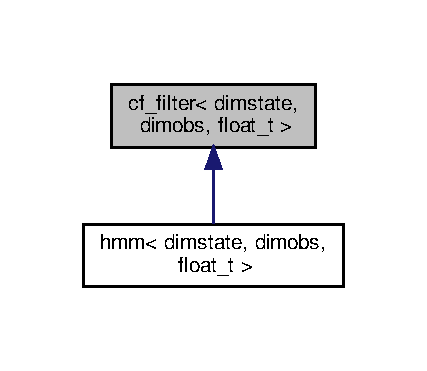
\includegraphics[width=350pt]{classcf__filter__inherit__graph}
\end{center}
\end{figure}
\subsection*{Public Types}
\begin{DoxyCompactItemize}
\item 
using \hyperlink{classcf__filter_ad4bce534d6b7a494dae851846037c94b}{ssv} = Eigen\+::\+Matrix$<$ float\+\_\+t, dimstate, 1 $>$
\item 
using \hyperlink{classcf__filter_a91d9961b2ecd202b1400c401434b392d}{osv} = Eigen\+::\+Matrix$<$ float\+\_\+t, dimstate, 1 $>$
\end{DoxyCompactItemize}
\subsection*{Public Member Functions}
\begin{DoxyCompactItemize}
\item 
\mbox{\Hypertarget{classcf__filter_afd3e7b3c1c0cc86257b406d494b0a7c9}\label{classcf__filter_afd3e7b3c1c0cc86257b406d494b0a7c9}} 
virtual \hyperlink{classcf__filter_afd3e7b3c1c0cc86257b406d494b0a7c9}{$\sim$cf\+\_\+filter} ()
\begin{DoxyCompactList}\small\item\em The (virtual) destructor. \end{DoxyCompactList}\item 
virtual float\+\_\+t \hyperlink{classcf__filter_a11b26307172bf94b8075ed2cdb8fc09c}{get\+Log\+Cond\+Like} () const =0
\begin{DoxyCompactList}\small\item\em returns the log of the most recent conditional likelihood \end{DoxyCompactList}\end{DoxyCompactItemize}


\subsection{Detailed Description}
\subsubsection*{template$<$size\+\_\+t dimstate, size\+\_\+t dimobs, typename float\+\_\+t$>$\newline
class cf\+\_\+filter$<$ dimstate, dimobs, float\+\_\+t $>$}

Abstract Base Class for all closed-\/form filters. 

\begin{DoxyAuthor}{Author}
taylor 
\end{DoxyAuthor}


\subsection{Member Typedef Documentation}
\mbox{\Hypertarget{classcf__filter_a91d9961b2ecd202b1400c401434b392d}\label{classcf__filter_a91d9961b2ecd202b1400c401434b392d}} 
\index{cf\+\_\+filter@{cf\+\_\+filter}!osv@{osv}}
\index{osv@{osv}!cf\+\_\+filter@{cf\+\_\+filter}}
\subsubsection{\texorpdfstring{osv}{osv}}
{\footnotesize\ttfamily template$<$size\+\_\+t dimstate, size\+\_\+t dimobs, typename float\+\_\+t$>$ \\
using \hyperlink{classcf__filter}{cf\+\_\+filter}$<$ dimstate, dimobs, float\+\_\+t $>$\+::\hyperlink{classcf__filter_a91d9961b2ecd202b1400c401434b392d}{osv} =  Eigen\+::\+Matrix$<$float\+\_\+t,dimstate,1$>$}

\char`\"{}observation size vector\char`\"{} type alias for linear algebra stuff \mbox{\Hypertarget{classcf__filter_ad4bce534d6b7a494dae851846037c94b}\label{classcf__filter_ad4bce534d6b7a494dae851846037c94b}} 
\index{cf\+\_\+filter@{cf\+\_\+filter}!ssv@{ssv}}
\index{ssv@{ssv}!cf\+\_\+filter@{cf\+\_\+filter}}
\subsubsection{\texorpdfstring{ssv}{ssv}}
{\footnotesize\ttfamily template$<$size\+\_\+t dimstate, size\+\_\+t dimobs, typename float\+\_\+t$>$ \\
using \hyperlink{classcf__filter}{cf\+\_\+filter}$<$ dimstate, dimobs, float\+\_\+t $>$\+::\hyperlink{classcf__filter_ad4bce534d6b7a494dae851846037c94b}{ssv} =  Eigen\+::\+Matrix$<$float\+\_\+t,dimstate,1$>$}

\char`\"{}state size vector\char`\"{} type alias for linear algebra stuff 

\subsection{Member Function Documentation}
\mbox{\Hypertarget{classcf__filter_a11b26307172bf94b8075ed2cdb8fc09c}\label{classcf__filter_a11b26307172bf94b8075ed2cdb8fc09c}} 
\index{cf\+\_\+filter@{cf\+\_\+filter}!get\+Log\+Cond\+Like@{get\+Log\+Cond\+Like}}
\index{get\+Log\+Cond\+Like@{get\+Log\+Cond\+Like}!cf\+\_\+filter@{cf\+\_\+filter}}
\subsubsection{\texorpdfstring{get\+Log\+Cond\+Like()}{getLogCondLike()}}
{\footnotesize\ttfamily template$<$size\+\_\+t dimstate, size\+\_\+t dimobs, typename float\+\_\+t$>$ \\
virtual float\+\_\+t \hyperlink{classcf__filter}{cf\+\_\+filter}$<$ dimstate, dimobs, float\+\_\+t $>$\+::get\+Log\+Cond\+Like (\begin{DoxyParamCaption}{ }\end{DoxyParamCaption}) const\hspace{0.3cm}{\ttfamily [pure virtual]}}



returns the log of the most recent conditional likelihood 

\begin{DoxyReturn}{Returns}
log p(y\+\_\+t $\vert$ y\+\_\+\{1\+:t-\/1\}) or log p(y\+\_\+1) 
\end{DoxyReturn}


Implemented in \hyperlink{classmultivGamFilter_ae32c76dd1096041f358962f93de64a99}{multiv\+Gam\+Filter$<$ dim\+\_\+obs, dim\+\_\+pred, float\+\_\+t $>$}, \hyperlink{classgamFilter_a8849fcc87e594367865c14767b8849e8}{gam\+Filter$<$ dim\+\_\+pred, float\+\_\+t $>$}, \hyperlink{classhmm_a588f2aed002614e75f523213eba1b290}{hmm$<$ dimstate, dimobs, float\+\_\+t $>$}, and \hyperlink{classkalman_aaf359a2d65f4f0ae8eb26603205b6f9b}{kalman$<$ dimstate, dimobs, diminput, float\+\_\+t $>$}.



The documentation for this class was generated from the following file\+:\begin{DoxyCompactItemize}
\item 
include/\hyperlink{cf__filters_8h}{cf\+\_\+filters.\+h}\end{DoxyCompactItemize}

\hypertarget{classForwardMod}{}\section{Forward\+Mod$<$ dimx, dimy, float\+\_\+t $>$ Class Template Reference}
\label{classForwardMod}\index{Forward\+Mod$<$ dimx, dimy, float\+\_\+t $>$@{Forward\+Mod$<$ dimx, dimy, float\+\_\+t $>$}}


{\ttfamily \#include $<$pf\+\_\+base.\+h$>$}

\subsection*{Public Types}
\begin{DoxyCompactItemize}
\item 
\mbox{\Hypertarget{classForwardMod_a32e8e8c3491d98db68e64cdca5bd05d9}\label{classForwardMod_a32e8e8c3491d98db68e64cdca5bd05d9}} 
using {\bfseries ssv} = Eigen\+::\+Matrix$<$ float\+\_\+t, dimx, 1 $>$
\item 
\mbox{\Hypertarget{classForwardMod_a81a5afb13a81b2ebb8196d626fa3f261}\label{classForwardMod_a81a5afb13a81b2ebb8196d626fa3f261}} 
using {\bfseries osv} = Eigen\+::\+Matrix$<$ float\+\_\+t, dimy, 1 $>$
\item 
\mbox{\Hypertarget{classForwardMod_a9d17ccfbab8e42cf70cd61c2f2c1844f}\label{classForwardMod_a9d17ccfbab8e42cf70cd61c2f2c1844f}} 
using {\bfseries a\+Pair} = std\+::pair$<$ std\+::vector$<$ ssv $>$, std\+::vector$<$ osv $>$ $>$
\end{DoxyCompactItemize}
\subsection*{Public Member Functions}
\begin{DoxyCompactItemize}
\item 
\mbox{\Hypertarget{classForwardMod_a374c715382620bef4475b233340dcbbc}\label{classForwardMod_a374c715382620bef4475b233340dcbbc}} 
a\+Pair \hyperlink{classForwardMod_a374c715382620bef4475b233340dcbbc}{sim\+\_\+forward} (unsigned int T)
\begin{DoxyCompactList}\small\item\em simulates forward through time \end{DoxyCompactList}\item 
virtual ssv \hyperlink{classForwardMod_aa768950ea619560a820905eb71eed82c}{mu\+Samp} ()=0
\begin{DoxyCompactList}\small\item\em samples from the first time\textquotesingle{}s state distribution \end{DoxyCompactList}\item 
virtual ssv \hyperlink{classForwardMod_aa46752032b11a6ac76cd01e13780a932}{f\+Samp} (const ssv \&xtm1)=0
\begin{DoxyCompactList}\small\item\em returns a sample from the latent Markov transition \end{DoxyCompactList}\item 
virtual osv \hyperlink{classForwardMod_a3264f80eae33f89a504cdb25634cadda}{g\+Samp} (const ssv \&xt)=0
\begin{DoxyCompactList}\small\item\em returns a sample for the observed series \end{DoxyCompactList}\end{DoxyCompactItemize}


\subsection{Detailed Description}
\subsubsection*{template$<$size\+\_\+t dimx, size\+\_\+t dimy, typename float\+\_\+t$>$\newline
class Forward\+Mod$<$ dimx, dimy, float\+\_\+t $>$}

\begin{DoxyAuthor}{Author}
t 
\end{DoxyAuthor}


\subsection{Member Function Documentation}
\mbox{\Hypertarget{classForwardMod_aa46752032b11a6ac76cd01e13780a932}\label{classForwardMod_aa46752032b11a6ac76cd01e13780a932}} 
\index{Forward\+Mod@{Forward\+Mod}!f\+Samp@{f\+Samp}}
\index{f\+Samp@{f\+Samp}!Forward\+Mod@{Forward\+Mod}}
\subsubsection{\texorpdfstring{f\+Samp()}{fSamp()}}
{\footnotesize\ttfamily template$<$size\+\_\+t dimx, size\+\_\+t dimy, typename float\+\_\+t $>$ \\
virtual ssv \hyperlink{classForwardMod}{Forward\+Mod}$<$ dimx, dimy, float\+\_\+t $>$\+::f\+Samp (\begin{DoxyParamCaption}\item[{const ssv \&}]{xtm1 }\end{DoxyParamCaption})\hspace{0.3cm}{\ttfamily [pure virtual]}}



returns a sample from the latent Markov transition 

\begin{DoxyReturn}{Returns}
a state-\/sized vector for the xt sample 
\end{DoxyReturn}
\mbox{\Hypertarget{classForwardMod_a3264f80eae33f89a504cdb25634cadda}\label{classForwardMod_a3264f80eae33f89a504cdb25634cadda}} 
\index{Forward\+Mod@{Forward\+Mod}!g\+Samp@{g\+Samp}}
\index{g\+Samp@{g\+Samp}!Forward\+Mod@{Forward\+Mod}}
\subsubsection{\texorpdfstring{g\+Samp()}{gSamp()}}
{\footnotesize\ttfamily template$<$size\+\_\+t dimx, size\+\_\+t dimy, typename float\+\_\+t $>$ \\
virtual osv \hyperlink{classForwardMod}{Forward\+Mod}$<$ dimx, dimy, float\+\_\+t $>$\+::g\+Samp (\begin{DoxyParamCaption}\item[{const ssv \&}]{xt }\end{DoxyParamCaption})\hspace{0.3cm}{\ttfamily [pure virtual]}}



returns a sample for the observed series 

\begin{DoxyReturn}{Returns}

\end{DoxyReturn}
\mbox{\Hypertarget{classForwardMod_aa768950ea619560a820905eb71eed82c}\label{classForwardMod_aa768950ea619560a820905eb71eed82c}} 
\index{Forward\+Mod@{Forward\+Mod}!mu\+Samp@{mu\+Samp}}
\index{mu\+Samp@{mu\+Samp}!Forward\+Mod@{Forward\+Mod}}
\subsubsection{\texorpdfstring{mu\+Samp()}{muSamp()}}
{\footnotesize\ttfamily template$<$size\+\_\+t dimx, size\+\_\+t dimy, typename float\+\_\+t $>$ \\
virtual ssv \hyperlink{classForwardMod}{Forward\+Mod}$<$ dimx, dimy, float\+\_\+t $>$\+::mu\+Samp (\begin{DoxyParamCaption}{ }\end{DoxyParamCaption})\hspace{0.3cm}{\ttfamily [pure virtual]}}



samples from the first time\textquotesingle{}s state distribution 

\begin{DoxyReturn}{Returns}
a state-\/sized vector for the x1 sample 
\end{DoxyReturn}


The documentation for this class was generated from the following file\+:\begin{DoxyCompactItemize}
\item 
include/pf/\hyperlink{pf__base_8h}{pf\+\_\+base.\+h}\end{DoxyCompactItemize}

\hypertarget{classgamFilter}{}\section{gam\+Filter$<$ dim\+\_\+pred, float\+\_\+t $>$ Class Template Reference}
\label{classgamFilter}\index{gam\+Filter$<$ dim\+\_\+pred, float\+\_\+t $>$@{gam\+Filter$<$ dim\+\_\+pred, float\+\_\+t $>$}}


A class template for Gamma filtering.  




{\ttfamily \#include $<$cf\+\_\+filters.\+h$>$}



Inheritance diagram for gam\+Filter$<$ dim\+\_\+pred, float\+\_\+t $>$\+:
\nopagebreak
\begin{figure}[H]
\begin{center}
\leavevmode
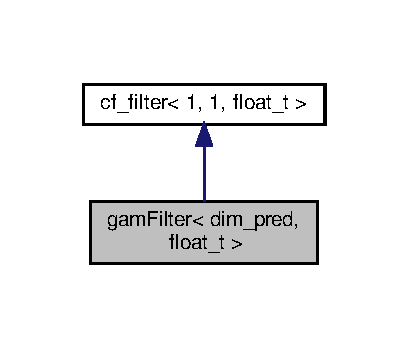
\includegraphics[width=196pt]{classgamFilter__inherit__graph}
\end{center}
\end{figure}


Collaboration diagram for gam\+Filter$<$ dim\+\_\+pred, float\+\_\+t $>$\+:
\nopagebreak
\begin{figure}[H]
\begin{center}
\leavevmode
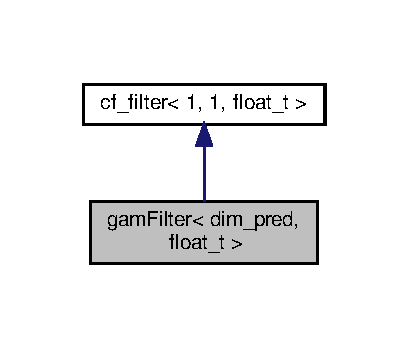
\includegraphics[width=196pt]{classgamFilter__coll__graph}
\end{center}
\end{figure}
\subsection*{Public Types}
\begin{DoxyCompactItemize}
\item 
\mbox{\Hypertarget{classgamFilter_ae43550158ad06de3a1829d5cb491b3fc}\label{classgamFilter_ae43550158ad06de3a1829d5cb491b3fc}} 
using \hyperlink{classgamFilter_ae43550158ad06de3a1829d5cb491b3fc}{psv} = Eigen\+::\+Matrix$<$ float\+\_\+t, dim\+\_\+pred, 1 $>$
\begin{DoxyCompactList}\small\item\em \char`\"{}predictor size vector\char`\"{} \end{DoxyCompactList}\item 
\mbox{\Hypertarget{classgamFilter_ab8cbe50cc21d9a9474c0e2b9b45a6162}\label{classgamFilter_ab8cbe50cc21d9a9474c0e2b9b45a6162}} 
using \hyperlink{classgamFilter_ab8cbe50cc21d9a9474c0e2b9b45a6162}{tsv} = Eigen\+::\+Matrix$<$ float\+\_\+t, 2, 1 $>$
\begin{DoxyCompactList}\small\item\em \char`\"{}two by 1 vector\char`\"{} \end{DoxyCompactList}\end{DoxyCompactItemize}
\subsection*{Public Member Functions}
\begin{DoxyCompactItemize}
\item 
\hyperlink{classgamFilter_af412e3430594dafd0779363c1664d5f8}{gam\+Filter} (const float\+\_\+t \&n\+One\+Tilde, const float\+\_\+t \&d\+One\+Tilde)
\begin{DoxyCompactList}\small\item\em Default constructor. \end{DoxyCompactList}\item 
\mbox{\Hypertarget{classgamFilter_af4f4009a88b82bb277f6ea9012fef940}\label{classgamFilter_af4f4009a88b82bb277f6ea9012fef940}} 
virtual \hyperlink{classgamFilter_af4f4009a88b82bb277f6ea9012fef940}{$\sim$gam\+Filter} ()
\begin{DoxyCompactList}\small\item\em The (virtual) desuctor. \end{DoxyCompactList}\item 
float\+\_\+t \hyperlink{classgamFilter_a8849fcc87e594367865c14767b8849e8}{get\+Log\+Cond\+Like} () const
\begin{DoxyCompactList}\small\item\em Get the latest conditional likelihood. \end{DoxyCompactList}\item 
\hyperlink{classgamFilter_ab8cbe50cc21d9a9474c0e2b9b45a6162}{tsv} \hyperlink{classgamFilter_a1e76b015d5319ab1ce188848b525927a}{get\+Filter\+Vec} () const
\begin{DoxyCompactList}\small\item\em Get the current filter vector. \end{DoxyCompactList}\item 
void \hyperlink{classgamFilter_af6a33d3fb634803c3b54521defb15b28}{update} (const float\+\_\+t \&yt, const \hyperlink{classgamFilter_ae43550158ad06de3a1829d5cb491b3fc}{psv} \&xt, const \hyperlink{classgamFilter_ae43550158ad06de3a1829d5cb491b3fc}{psv} \&beta, const float\+\_\+t \&sigma\+Squared, const float\+\_\+t \&delta)
\begin{DoxyCompactList}\small\item\em Perform a filtering update. \end{DoxyCompactList}\end{DoxyCompactItemize}
\subsection*{Private Attributes}
\begin{DoxyCompactItemize}
\item 
\mbox{\Hypertarget{classgamFilter_a6ab069a63962551ef8b580cb9eb681c9}\label{classgamFilter_a6ab069a63962551ef8b580cb9eb681c9}} 
\hyperlink{classgamFilter_ab8cbe50cc21d9a9474c0e2b9b45a6162}{tsv} \hyperlink{classgamFilter_a6ab069a63962551ef8b580cb9eb681c9}{m\+\_\+filt\+Vec}
\begin{DoxyCompactList}\small\item\em filter vector (shape and rate) \end{DoxyCompactList}\item 
\mbox{\Hypertarget{classgamFilter_a15774fb5c9c20bff2f0f99cf52a2445f}\label{classgamFilter_a15774fb5c9c20bff2f0f99cf52a2445f}} 
float\+\_\+t \hyperlink{classgamFilter_a15774fb5c9c20bff2f0f99cf52a2445f}{m\+\_\+last\+Log\+Cond\+Like}
\begin{DoxyCompactList}\small\item\em last log of the conditional likelihood \end{DoxyCompactList}\item 
\mbox{\Hypertarget{classgamFilter_a6bf29aaf7b43bb446821f06ea643df3f}\label{classgamFilter_a6bf29aaf7b43bb446821f06ea643df3f}} 
bool \hyperlink{classgamFilter_a6bf29aaf7b43bb446821f06ea643df3f}{m\+\_\+fresh}
\begin{DoxyCompactList}\small\item\em has data been observed? \end{DoxyCompactList}\end{DoxyCompactItemize}


\subsection{Detailed Description}
\subsubsection*{template$<$size\+\_\+t dim\+\_\+pred, typename float\+\_\+t$>$\newline
class gam\+Filter$<$ dim\+\_\+pred, float\+\_\+t $>$}

A class template for Gamma filtering. 

\begin{DoxyAuthor}{Author}
taylor 
\end{DoxyAuthor}


\subsection{Constructor \& Destructor Documentation}
\mbox{\Hypertarget{classgamFilter_af412e3430594dafd0779363c1664d5f8}\label{classgamFilter_af412e3430594dafd0779363c1664d5f8}} 
\index{gam\+Filter@{gam\+Filter}!gam\+Filter@{gam\+Filter}}
\index{gam\+Filter@{gam\+Filter}!gam\+Filter@{gam\+Filter}}
\subsubsection{\texorpdfstring{gam\+Filter()}{gamFilter()}}
{\footnotesize\ttfamily template$<$size\+\_\+t dim\+\_\+pred, typename float\+\_\+t $>$ \\
\hyperlink{classgamFilter}{gam\+Filter}$<$ dim\+\_\+pred, float\+\_\+t $>$\+::\hyperlink{classgamFilter}{gam\+Filter} (\begin{DoxyParamCaption}\item[{const float\+\_\+t \&}]{n\+One\+Tilde,  }\item[{const float\+\_\+t \&}]{d\+One\+Tilde }\end{DoxyParamCaption})}



Default constructor. 

Need ths fir constructing default std\+::array$<$$>$s. Fills all vectors and matrices with zeros.\+Constructor


\begin{DoxyParams}{Parameters}
{\em n\+One\+Tilde} & degrees of freedom for time 1 prior. \\
\hline
{\em d\+One\+Tilde} & rate parameter for time 1 prior. \\
\hline
\end{DoxyParams}


\subsection{Member Function Documentation}
\mbox{\Hypertarget{classgamFilter_a1e76b015d5319ab1ce188848b525927a}\label{classgamFilter_a1e76b015d5319ab1ce188848b525927a}} 
\index{gam\+Filter@{gam\+Filter}!get\+Filter\+Vec@{get\+Filter\+Vec}}
\index{get\+Filter\+Vec@{get\+Filter\+Vec}!gam\+Filter@{gam\+Filter}}
\subsubsection{\texorpdfstring{get\+Filter\+Vec()}{getFilterVec()}}
{\footnotesize\ttfamily template$<$size\+\_\+t dim\+\_\+pred, typename float\+\_\+t $>$ \\
auto \hyperlink{classgamFilter}{gam\+Filter}$<$ dim\+\_\+pred, float\+\_\+t $>$\+::get\+Filter\+Vec (\begin{DoxyParamCaption}{ }\end{DoxyParamCaption}) const}



Get the current filter vector. 

get the current filtering distribution. First element is the shape, second is the rate. \begin{DoxyReturn}{Returns}
a vector of the shape and rate parameters of f(p\+\_\+t $\vert$ y\+\_\+\{1\+:t\}) 
\end{DoxyReturn}
\mbox{\Hypertarget{classgamFilter_a8849fcc87e594367865c14767b8849e8}\label{classgamFilter_a8849fcc87e594367865c14767b8849e8}} 
\index{gam\+Filter@{gam\+Filter}!get\+Log\+Cond\+Like@{get\+Log\+Cond\+Like}}
\index{get\+Log\+Cond\+Like@{get\+Log\+Cond\+Like}!gam\+Filter@{gam\+Filter}}
\subsubsection{\texorpdfstring{get\+Log\+Cond\+Like()}{getLogCondLike()}}
{\footnotesize\ttfamily template$<$size\+\_\+t dim\+\_\+pred, typename float\+\_\+t $>$ \\
auto \hyperlink{classgamFilter}{gam\+Filter}$<$ dim\+\_\+pred, float\+\_\+t $>$\+::get\+Log\+Cond\+Like (\begin{DoxyParamCaption}{ }\end{DoxyParamCaption}) const\hspace{0.3cm}{\ttfamily [virtual]}}



Get the latest conditional likelihood. 

\begin{DoxyReturn}{Returns}
the latest conditional likelihood. 
\end{DoxyReturn}


Implements \hyperlink{classcf__filter_a11b26307172bf94b8075ed2cdb8fc09c}{cf\+\_\+filter$<$ 1, 1, float\+\_\+t $>$}.

\mbox{\Hypertarget{classgamFilter_af6a33d3fb634803c3b54521defb15b28}\label{classgamFilter_af6a33d3fb634803c3b54521defb15b28}} 
\index{gam\+Filter@{gam\+Filter}!update@{update}}
\index{update@{update}!gam\+Filter@{gam\+Filter}}
\subsubsection{\texorpdfstring{update()}{update()}}
{\footnotesize\ttfamily template$<$size\+\_\+t dim\+\_\+pred, typename float\+\_\+t $>$ \\
void \hyperlink{classgamFilter}{gam\+Filter}$<$ dim\+\_\+pred, float\+\_\+t $>$\+::update (\begin{DoxyParamCaption}\item[{const float\+\_\+t \&}]{yt,  }\item[{const \hyperlink{classgamFilter_ae43550158ad06de3a1829d5cb491b3fc}{psv} \&}]{xt,  }\item[{const \hyperlink{classgamFilter_ae43550158ad06de3a1829d5cb491b3fc}{psv} \&}]{beta,  }\item[{const float\+\_\+t \&}]{sigma\+Squared,  }\item[{const float\+\_\+t \&}]{delta }\end{DoxyParamCaption})}



Perform a filtering update. 

Perform a Gamma filter update. 
\begin{DoxyParams}{Parameters}
{\em yt} & the most recent dependent random variable \\
\hline
{\em xt} & the most recent predictor vector \\
\hline
{\em beta} & the beta vector \\
\hline
{\em sigma\+Squared} & the observation variance scale parameter. \\
\hline
{\em delta} & between 0 and 1 the discount parameter \\
\hline
\end{DoxyParams}


The documentation for this class was generated from the following file\+:\begin{DoxyCompactItemize}
\item 
include/\hyperlink{cf__filters_8h}{cf\+\_\+filters.\+h}\end{DoxyCompactItemize}

\hypertarget{classhmm}{}\section{hmm$<$ dimstate, dimobs $>$ Class Template Reference}
\label{classhmm}\index{hmm$<$ dimstate, dimobs $>$@{hmm$<$ dimstate, dimobs $>$}}


A class template for H\+MM filtering.  




{\ttfamily \#include $<$cf\+\_\+filters.\+h$>$}



Inheritance diagram for hmm$<$ dimstate, dimobs $>$\+:\nopagebreak
\begin{figure}[H]
\begin{center}
\leavevmode
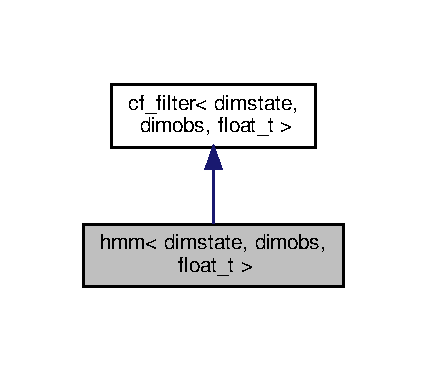
\includegraphics[width=211pt]{classhmm__inherit__graph}
\end{center}
\end{figure}


Collaboration diagram for hmm$<$ dimstate, dimobs $>$\+:\nopagebreak
\begin{figure}[H]
\begin{center}
\leavevmode
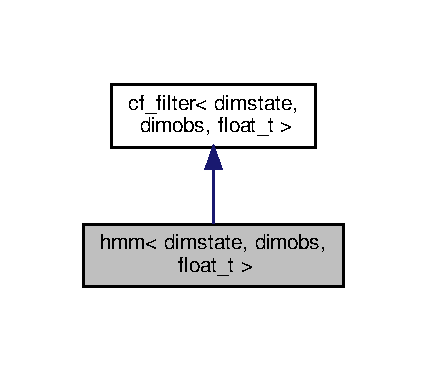
\includegraphics[width=211pt]{classhmm__coll__graph}
\end{center}
\end{figure}
\subsection*{Public Types}
\begin{DoxyCompactItemize}
\item 
using \hyperlink{classhmm_a4a536464d63f3e7b06ab867cde35fb6a}{ssv} = Eigen\+::\+Matrix$<$ double, dimstate, 1 $>$\hypertarget{classhmm_a4a536464d63f3e7b06ab867cde35fb6a}{}\label{classhmm_a4a536464d63f3e7b06ab867cde35fb6a}

\begin{DoxyCompactList}\small\item\em \char`\"{}state size vector\char`\"{} \end{DoxyCompactList}\item 
using \hyperlink{classhmm_a8b831550f17d3abfdbde1d9aadfdc861}{osv} = Eigen\+::\+Matrix$<$ double, dimobs, 1 $>$\hypertarget{classhmm_a8b831550f17d3abfdbde1d9aadfdc861}{}\label{classhmm_a8b831550f17d3abfdbde1d9aadfdc861}

\begin{DoxyCompactList}\small\item\em \char`\"{}observation size vector\char`\"{} \end{DoxyCompactList}\item 
using \hyperlink{classhmm_a1c1d1649a78ddbe6029556fd1e10d0ab}{ss\+Mat} = Eigen\+::\+Matrix$<$ double, dimstate, dimstate $>$\hypertarget{classhmm_a1c1d1649a78ddbe6029556fd1e10d0ab}{}\label{classhmm_a1c1d1649a78ddbe6029556fd1e10d0ab}

\begin{DoxyCompactList}\small\item\em \char`\"{}state size matrix\char`\"{} \end{DoxyCompactList}\end{DoxyCompactItemize}
\subsection*{Public Member Functions}
\begin{DoxyCompactItemize}
\item 
\hyperlink{classhmm_ae7ec1812c1ee0d8ed57eb6c3f62b92a1}{hmm} ()
\begin{DoxyCompactList}\small\item\em Default constructor. \end{DoxyCompactList}\item 
\hyperlink{classhmm_a3ad1950d8fcef28430da0bf435da0a77}{hmm} (const \hyperlink{classcf__filter_a5562e379d385df4d81c949e32d84ee19}{ssv} \&init\+State\+Distr, const \hyperlink{classhmm_a1c1d1649a78ddbe6029556fd1e10d0ab}{ss\+Mat} \&trans\+Mat)
\begin{DoxyCompactList}\small\item\em Constructor. \end{DoxyCompactList}\item 
double \hyperlink{classhmm_ab961ea54f4573a1b1c257162fb264cf7}{get\+Log\+Cond\+Like} () const 
\begin{DoxyCompactList}\small\item\em Get the latest conditional likelihood. \end{DoxyCompactList}\item 
\hyperlink{classcf__filter_a5562e379d385df4d81c949e32d84ee19}{ssv} \hyperlink{classhmm_a71547a134dce31e831004cace2ba4bd7}{get\+Filter\+Vec} () const 
\begin{DoxyCompactList}\small\item\em Get the current filter vector. \end{DoxyCompactList}\item 
void \hyperlink{classhmm_ae294c9e939f3484f00c943f505095971}{update} (const \hyperlink{classcf__filter_a5562e379d385df4d81c949e32d84ee19}{ssv} \&cond\+Dens\+Vec)
\begin{DoxyCompactList}\small\item\em Perform a H\+MM filter update. \end{DoxyCompactList}\end{DoxyCompactItemize}
\subsection*{Private Attributes}
\begin{DoxyCompactItemize}
\item 
\hyperlink{classcf__filter_a5562e379d385df4d81c949e32d84ee19}{ssv} \hyperlink{classhmm_a1d95a240203405976193cc9792b83a67}{m\+\_\+filt\+Vec}\hypertarget{classhmm_a1d95a240203405976193cc9792b83a67}{}\label{classhmm_a1d95a240203405976193cc9792b83a67}

\begin{DoxyCompactList}\small\item\em filter vector \end{DoxyCompactList}\item 
\hyperlink{classhmm_a1c1d1649a78ddbe6029556fd1e10d0ab}{ss\+Mat} \hyperlink{classhmm_a27c26b0248bafd930ff33278ec1c4c10}{m\+\_\+trans\+Mat\+Transpose}\hypertarget{classhmm_a27c26b0248bafd930ff33278ec1c4c10}{}\label{classhmm_a27c26b0248bafd930ff33278ec1c4c10}

\begin{DoxyCompactList}\small\item\em transition matrix \end{DoxyCompactList}\item 
double \hyperlink{classhmm_ad02a43632a0cc42b96730ddb0cf6d538}{m\+\_\+last\+Cond\+Like}\hypertarget{classhmm_ad02a43632a0cc42b96730ddb0cf6d538}{}\label{classhmm_ad02a43632a0cc42b96730ddb0cf6d538}

\begin{DoxyCompactList}\small\item\em last conditional likelihood \end{DoxyCompactList}\item 
bool \hyperlink{classhmm_ad5e43bdfcbdf90cc610a1d9148755c46}{m\+\_\+fresh}\hypertarget{classhmm_ad5e43bdfcbdf90cc610a1d9148755c46}{}\label{classhmm_ad5e43bdfcbdf90cc610a1d9148755c46}

\begin{DoxyCompactList}\small\item\em has data been observed? \end{DoxyCompactList}\end{DoxyCompactItemize}


\subsection{Detailed Description}
\subsubsection*{template$<$size\+\_\+t dimstate, size\+\_\+t dimobs$>$\\*
class hmm$<$ dimstate, dimobs $>$}

A class template for H\+MM filtering. 

\begin{DoxyAuthor}{Author}
taylor 
\end{DoxyAuthor}


\subsection{Constructor \& Destructor Documentation}
\index{hmm@{hmm}!hmm@{hmm}}
\index{hmm@{hmm}!hmm@{hmm}}
\subsubsection[{\texorpdfstring{hmm()}{hmm()}}]{\setlength{\rightskip}{0pt plus 5cm}template$<$size\+\_\+t dimstate, size\+\_\+t dimobs$>$ {\bf hmm}$<$ dimstate, dimobs $>$\+::{\bf hmm} (
\begin{DoxyParamCaption}
{}
\end{DoxyParamCaption}
)}\hypertarget{classhmm_ae7ec1812c1ee0d8ed57eb6c3f62b92a1}{}\label{classhmm_ae7ec1812c1ee0d8ed57eb6c3f62b92a1}


Default constructor. 

Need ths fir constructing default std\+::array$<$$>$s. Fills all vectors and matrices with zeros. \index{hmm@{hmm}!hmm@{hmm}}
\index{hmm@{hmm}!hmm@{hmm}}
\subsubsection[{\texorpdfstring{hmm(const ssv \&init\+State\+Distr, const ss\+Mat \&trans\+Mat)}{hmm(const ssv &initStateDistr, const ssMat &transMat)}}]{\setlength{\rightskip}{0pt plus 5cm}template$<$size\+\_\+t dimstate, size\+\_\+t dimobs$>$ {\bf hmm}$<$ dimstate, dimobs $>$\+::{\bf hmm} (
\begin{DoxyParamCaption}
\item[{const {\bf ssv} \&}]{init\+State\+Distr, }
\item[{const {\bf ss\+Mat} \&}]{trans\+Mat}
\end{DoxyParamCaption}
)}\hypertarget{classhmm_a3ad1950d8fcef28430da0bf435da0a77}{}\label{classhmm_a3ad1950d8fcef28430da0bf435da0a77}


Constructor. 

allows specification of initstate distn and transition matrix. 
\begin{DoxyParams}{Parameters}
{\em init\+State\+Distr} & first time state prior distribution. \\
\hline
{\em trans\+Mat} & time homogeneous transition matrix. \\
\hline
\end{DoxyParams}


\subsection{Member Function Documentation}
\index{hmm@{hmm}!get\+Filter\+Vec@{get\+Filter\+Vec}}
\index{get\+Filter\+Vec@{get\+Filter\+Vec}!hmm@{hmm}}
\subsubsection[{\texorpdfstring{get\+Filter\+Vec() const }{getFilterVec() const }}]{\setlength{\rightskip}{0pt plus 5cm}template$<$size\+\_\+t dimstate, size\+\_\+t dimobs$>$ auto {\bf hmm}$<$ dimstate, dimobs $>$\+::get\+Filter\+Vec (
\begin{DoxyParamCaption}
{}
\end{DoxyParamCaption}
) const}\hypertarget{classhmm_a71547a134dce31e831004cace2ba4bd7}{}\label{classhmm_a71547a134dce31e831004cace2ba4bd7}


Get the current filter vector. 

get the current filter vector. \begin{DoxyReturn}{Returns}
a probability vector p(x\+\_\+t $\vert$ y\+\_\+\{1\+:t\}) 
\end{DoxyReturn}
\index{hmm@{hmm}!get\+Log\+Cond\+Like@{get\+Log\+Cond\+Like}}
\index{get\+Log\+Cond\+Like@{get\+Log\+Cond\+Like}!hmm@{hmm}}
\subsubsection[{\texorpdfstring{get\+Log\+Cond\+Like() const }{getLogCondLike() const }}]{\setlength{\rightskip}{0pt plus 5cm}template$<$size\+\_\+t dimstate, size\+\_\+t dimobs$>$ double {\bf hmm}$<$ dimstate, dimobs $>$\+::get\+Log\+Cond\+Like (
\begin{DoxyParamCaption}
{}
\end{DoxyParamCaption}
) const\hspace{0.3cm}{\ttfamily [virtual]}}\hypertarget{classhmm_ab961ea54f4573a1b1c257162fb264cf7}{}\label{classhmm_ab961ea54f4573a1b1c257162fb264cf7}


Get the latest conditional likelihood. 

\begin{DoxyReturn}{Returns}
the latest conditional likelihood. 
\end{DoxyReturn}


Implements \hyperlink{classcf__filter_a561b2979440ad273807f2ec16bc6f3ae}{cf\+\_\+filter$<$ dimstate, dimobs $>$}.

\index{hmm@{hmm}!update@{update}}
\index{update@{update}!hmm@{hmm}}
\subsubsection[{\texorpdfstring{update(const ssv \&cond\+Dens\+Vec)}{update(const ssv &condDensVec)}}]{\setlength{\rightskip}{0pt plus 5cm}template$<$size\+\_\+t dimstate, size\+\_\+t dimobs$>$ void {\bf hmm}$<$ dimstate, dimobs $>$\+::update (
\begin{DoxyParamCaption}
\item[{const {\bf ssv} \&}]{cond\+Dens\+Vec}
\end{DoxyParamCaption}
)}\hypertarget{classhmm_ae294c9e939f3484f00c943f505095971}{}\label{classhmm_ae294c9e939f3484f00c943f505095971}


Perform a H\+MM filter update. 

Perform a H\+MM filter update. 
\begin{DoxyParams}{Parameters}
{\em cond\+Dens\+Vec} & the vector (in x\+\_\+t) of p(y\+\_\+t$\vert$x\+\_\+t) \\
\hline
\end{DoxyParams}


The documentation for this class was generated from the following file\+:\begin{DoxyCompactItemize}
\item 
include/\hyperlink{cf__filters_8h}{cf\+\_\+filters.\+h}\end{DoxyCompactItemize}

\hypertarget{classrvsamp_1_1k__gen}{}\section{rvsamp\+:\+:k\+\_\+gen$<$ N $>$ Class Template Reference}
\label{classrvsamp_1_1k__gen}\index{rvsamp\+::k\+\_\+gen$<$ N $>$@{rvsamp\+::k\+\_\+gen$<$ N $>$}}


A class that performs sampling with replacement (useful for the index sampler in an \hyperlink{classAPF}{A\+PF})  




{\ttfamily \#include $<$rv\+\_\+samp.\+h$>$}



Inheritance diagram for rvsamp\+:\+:k\+\_\+gen$<$ N $>$\+:\nopagebreak
\begin{figure}[H]
\begin{center}
\leavevmode
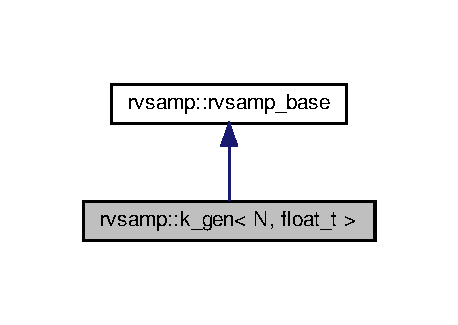
\includegraphics[width=219pt]{classrvsamp_1_1k__gen__inherit__graph}
\end{center}
\end{figure}


Collaboration diagram for rvsamp\+:\+:k\+\_\+gen$<$ N $>$\+:\nopagebreak
\begin{figure}[H]
\begin{center}
\leavevmode
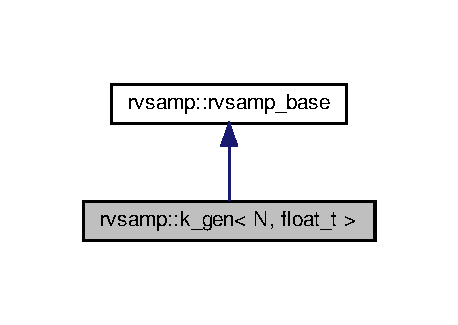
\includegraphics[width=219pt]{classrvsamp_1_1k__gen__coll__graph}
\end{center}
\end{figure}
\subsection*{Public Member Functions}
\begin{DoxyCompactItemize}
\item 
\hyperlink{classrvsamp_1_1k__gen_a3f3f0cd14ebf47d18796c713e834306c}{k\+\_\+gen} ()\hypertarget{classrvsamp_1_1k__gen_a3f3f0cd14ebf47d18796c713e834306c}{}\label{classrvsamp_1_1k__gen_a3f3f0cd14ebf47d18796c713e834306c}

\begin{DoxyCompactList}\small\item\em default constructor. only one available. \end{DoxyCompactList}\item 
std\+::array$<$ unsigned int, N $>$ \hyperlink{classrvsamp_1_1k__gen_a00221f2eab38faaf602a25b626f184d6}{sample} (const std\+::array$<$ double, N $>$ \&log\+Wts)
\begin{DoxyCompactList}\small\item\em sample N times from (0,1,...N-\/1) \end{DoxyCompactList}\end{DoxyCompactItemize}
\subsection*{Additional Inherited Members}


\subsection{Detailed Description}
\subsubsection*{template$<$size\+\_\+t N$>$\\*
class rvsamp\+::k\+\_\+gen$<$ N $>$}

A class that performs sampling with replacement (useful for the index sampler in an \hyperlink{classAPF}{A\+PF}) 

\begin{DoxyAuthor}{Author}
taylor 
\end{DoxyAuthor}


\subsection{Member Function Documentation}
\index{rvsamp\+::k\+\_\+gen@{rvsamp\+::k\+\_\+gen}!sample@{sample}}
\index{sample@{sample}!rvsamp\+::k\+\_\+gen@{rvsamp\+::k\+\_\+gen}}
\subsubsection[{\texorpdfstring{sample(const std\+::array$<$ double, N $>$ \&log\+Wts)}{sample(const std::array< double, N > &logWts)}}]{\setlength{\rightskip}{0pt plus 5cm}template$<$size\+\_\+t N$>$ std\+::array$<$ unsigned int, N $>$ {\bf rvsamp\+::k\+\_\+gen}$<$ N $>$\+::sample (
\begin{DoxyParamCaption}
\item[{const std\+::array$<$ double, N $>$ \&}]{log\+Wts}
\end{DoxyParamCaption}
)}\hypertarget{classrvsamp_1_1k__gen_a00221f2eab38faaf602a25b626f184d6}{}\label{classrvsamp_1_1k__gen_a00221f2eab38faaf602a25b626f184d6}


sample N times from (0,1,...N-\/1) 


\begin{DoxyParams}{Parameters}
{\em log\+Wts} & possibly unnormalized type std\+::array$<$double, N$>$ \\
\hline
\end{DoxyParams}
\begin{DoxyReturn}{Returns}
the integers in a std\+::array$<$unsigned int, N$>$ 
\end{DoxyReturn}


The documentation for this class was generated from the following file\+:\begin{DoxyCompactItemize}
\item 
include/\hyperlink{rv__samp_8h}{rv\+\_\+samp.\+h}\end{DoxyCompactItemize}

\hypertarget{classkalman}{}\section{kalman$<$ dimstate, dimobs, diminput, float\+\_\+t $>$ Class Template Reference}
\label{classkalman}\index{kalman$<$ dimstate, dimobs, diminput, float\+\_\+t $>$@{kalman$<$ dimstate, dimobs, diminput, float\+\_\+t $>$}}


A class template for Kalman filtering.  




{\ttfamily \#include $<$cf\+\_\+filters.\+h$>$}



Inheritance diagram for kalman$<$ dimstate, dimobs, diminput, float\+\_\+t $>$\+:\nopagebreak
\begin{figure}[H]
\begin{center}
\leavevmode
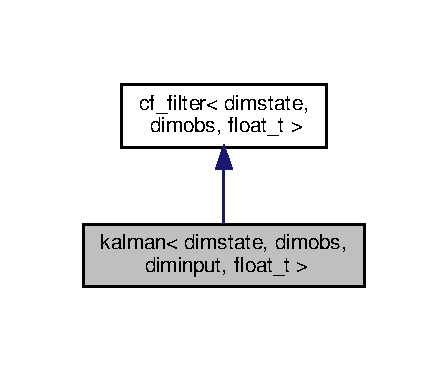
\includegraphics[width=215pt]{classkalman__inherit__graph}
\end{center}
\end{figure}


Collaboration diagram for kalman$<$ dimstate, dimobs, diminput, float\+\_\+t $>$\+:\nopagebreak
\begin{figure}[H]
\begin{center}
\leavevmode
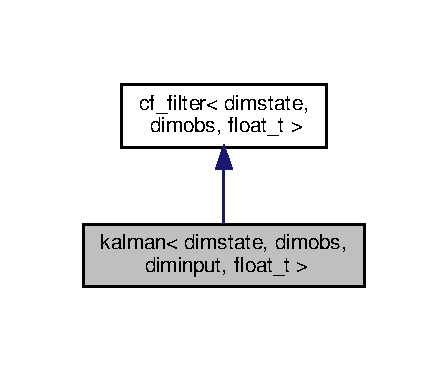
\includegraphics[width=215pt]{classkalman__coll__graph}
\end{center}
\end{figure}
\subsection*{Public Types}
\begin{DoxyCompactItemize}
\item 
using \hyperlink{classkalman_a732cf05b5ddd106cfdafc324d03f756e}{ssv} = Eigen\+::\+Matrix$<$ float\+\_\+t, dimstate, 1 $>$
\item 
using \hyperlink{classkalman_a0172e54797a5d5b0acc4168894adc6d5}{osv} = Eigen\+::\+Matrix$<$ float\+\_\+t, dimobs, 1 $>$
\item 
using \hyperlink{classkalman_abc570ce1b06e8a96a334f9226dfbce77}{isv} = Eigen\+::\+Matrix$<$ float\+\_\+t, diminput, 1 $>$
\item 
using \hyperlink{classkalman_a581550d9aba33245fb496b22a834831c}{ss\+Mat} = Eigen\+::\+Matrix$<$ float\+\_\+t, dimstate, dimstate $>$
\item 
using \hyperlink{classkalman_a28ffd71604fac7b25492b1b43379e046}{os\+Mat} = Eigen\+::\+Matrix$<$ float\+\_\+t, dimobs, dimobs $>$
\item 
using \hyperlink{classkalman_ab024c795f585385ee14aea92a5dccfbc}{si\+Mat} = Eigen\+::\+Matrix$<$ float\+\_\+t, dimstate, diminput $>$
\item 
using \hyperlink{classkalman_a35298f18f0b699f700e2d55d94bf54fc}{oi\+Mat} = Eigen\+::\+Matrix$<$ float\+\_\+t, dimobs, diminput $>$
\item 
using \hyperlink{classkalman_a13c0f71cc509326e1493982e9f23ebfc}{obs\+State\+Size\+Mat} = Eigen\+::\+Matrix$<$ float\+\_\+t, dimobs, dimstate $>$
\item 
using \hyperlink{classkalman_a44779d7ee7b8c12ca08e9dac4112906c}{state\+Obs\+Size\+Mat} = Eigen\+::\+Matrix$<$ float\+\_\+t, dimstate, dimobs $>$
\end{DoxyCompactItemize}
\subsection*{Public Member Functions}
\begin{DoxyCompactItemize}
\item 
\hyperlink{classkalman_a8b05d79f154bf5669457a3e95f7323d5}{kalman} ()
\begin{DoxyCompactList}\small\item\em Default constructor. \end{DoxyCompactList}\item 
\hyperlink{classkalman_a91ec8bcb52e26df651001d8f8e574373}{kalman} (const \hyperlink{classcf__filter_ad4bce534d6b7a494dae851846037c94b}{ssv} \&init\+State\+Mean, const \hyperlink{classkalman_a581550d9aba33245fb496b22a834831c}{ss\+Mat} \&init\+State\+Var)
\begin{DoxyCompactList}\small\item\em Non-\/default constructor. \end{DoxyCompactList}\item 
\mbox{\Hypertarget{classkalman_ae9284574db789ce2d961b6fe62d80fac}\label{classkalman_ae9284574db789ce2d961b6fe62d80fac}} 
virtual \hyperlink{classkalman_ae9284574db789ce2d961b6fe62d80fac}{$\sim$kalman} ()
\begin{DoxyCompactList}\small\item\em The (virtual) destructor. \end{DoxyCompactList}\item 
float\+\_\+t \hyperlink{classkalman_aaf359a2d65f4f0ae8eb26603205b6f9b}{get\+Log\+Cond\+Like} () const
\begin{DoxyCompactList}\small\item\em returns the log of the latest conditional likelihood. \end{DoxyCompactList}\item 
\hyperlink{classcf__filter_ad4bce534d6b7a494dae851846037c94b}{ssv} \hyperlink{classkalman_a247a3cef3a1fcec8c858372014276acf}{get\+Filt\+Mean} () const
\begin{DoxyCompactList}\small\item\em Get the current filter mean. \end{DoxyCompactList}\item 
\hyperlink{classkalman_a581550d9aba33245fb496b22a834831c}{ss\+Mat} \hyperlink{classkalman_af88f227e98383b222dc765b11df626c1}{get\+Filt\+Var} () const
\begin{DoxyCompactList}\small\item\em Get the current filter variance-\/covariance matrix. \end{DoxyCompactList}\item 
\hyperlink{classcf__filter_a91d9961b2ecd202b1400c401434b392d}{osv} \hyperlink{classkalman_a9578d69543a3e756275e61a69ad9f1ac}{get\+Pred\+Y\+Mean} (const \hyperlink{classkalman_a581550d9aba33245fb496b22a834831c}{ss\+Mat} \&state\+Trans, const \hyperlink{classkalman_a13c0f71cc509326e1493982e9f23ebfc}{obs\+State\+Size\+Mat} \&obs\+Mat, const \hyperlink{classkalman_ab024c795f585385ee14aea92a5dccfbc}{si\+Mat} \&state\+Inpt\+Affector, const \hyperlink{classkalman_a35298f18f0b699f700e2d55d94bf54fc}{oi\+Mat} \&obs\+Inpt\+Affector, const \hyperlink{classkalman_abc570ce1b06e8a96a334f9226dfbce77}{isv} \&input\+Data) const
\begin{DoxyCompactList}\small\item\em get the one-\/step-\/ahead point forecast for y \end{DoxyCompactList}\item 
\hyperlink{classkalman_a28ffd71604fac7b25492b1b43379e046}{os\+Mat} \hyperlink{classkalman_a029d34d75a517bc82d097bb9e289497f}{get\+Pred\+Y\+Var} (const \hyperlink{classkalman_a581550d9aba33245fb496b22a834831c}{ss\+Mat} \&state\+Trans, const \hyperlink{classkalman_a581550d9aba33245fb496b22a834831c}{ss\+Mat} \&chol\+State\+Var, const \hyperlink{classkalman_a13c0f71cc509326e1493982e9f23ebfc}{obs\+State\+Size\+Mat} \&obs\+Mat, const \hyperlink{classkalman_a28ffd71604fac7b25492b1b43379e046}{os\+Mat} \&chol\+Obs\+Var) const
\begin{DoxyCompactList}\small\item\em get the one-\/step-\/ahead forecast variance \end{DoxyCompactList}\item 
void \hyperlink{classkalman_af6da5b13d55eee01cd609c1bc694b3ef}{update} (const \hyperlink{classcf__filter_a91d9961b2ecd202b1400c401434b392d}{osv} \&yt, const \hyperlink{classkalman_a581550d9aba33245fb496b22a834831c}{ss\+Mat} \&state\+Trans, const \hyperlink{classkalman_a581550d9aba33245fb496b22a834831c}{ss\+Mat} \&chol\+State\+Var, const \hyperlink{classkalman_ab024c795f585385ee14aea92a5dccfbc}{si\+Mat} \&state\+Inpt\+Affector, const \hyperlink{classkalman_abc570ce1b06e8a96a334f9226dfbce77}{isv} \&input\+Data, const \hyperlink{classkalman_a13c0f71cc509326e1493982e9f23ebfc}{obs\+State\+Size\+Mat} \&obs\+Mat, const \hyperlink{classkalman_a35298f18f0b699f700e2d55d94bf54fc}{oi\+Mat} \&obs\+Inpt\+Affector, const \hyperlink{classkalman_a28ffd71604fac7b25492b1b43379e046}{os\+Mat} \&chol\+Obs\+Var)
\begin{DoxyCompactList}\small\item\em Perform a Kalman filter predict-\/and-\/update. \end{DoxyCompactList}\end{DoxyCompactItemize}
\subsection*{Private Member Functions}
\begin{DoxyCompactItemize}
\item 
void \hyperlink{classkalman_af4a5d62ffbd478fedfb040cb9e4fcb24}{update\+Prior} (const \hyperlink{classkalman_a581550d9aba33245fb496b22a834831c}{ss\+Mat} \&state\+Trans\+Mat, const \hyperlink{classkalman_a581550d9aba33245fb496b22a834831c}{ss\+Mat} \&chol\+State\+Var, const \hyperlink{classkalman_ab024c795f585385ee14aea92a5dccfbc}{si\+Mat} \&state\+Inpt\+Affector, const \hyperlink{classkalman_abc570ce1b06e8a96a334f9226dfbce77}{isv} \&input\+Data)
\begin{DoxyCompactList}\small\item\em Predicts the next state. \end{DoxyCompactList}\item 
void \hyperlink{classkalman_a74e4c7efe17efc0b7ae6111d4bb53765}{update\+Posterior} (const \hyperlink{classcf__filter_a91d9961b2ecd202b1400c401434b392d}{osv} \&yt, const \hyperlink{classkalman_a13c0f71cc509326e1493982e9f23ebfc}{obs\+State\+Size\+Mat} \&obs\+Mat, const \hyperlink{classkalman_a35298f18f0b699f700e2d55d94bf54fc}{oi\+Mat} \&obs\+Inpt\+Affector, const \hyperlink{classkalman_abc570ce1b06e8a96a334f9226dfbce77}{isv} \&input\+Data, const \hyperlink{classkalman_a28ffd71604fac7b25492b1b43379e046}{os\+Mat} \&chol\+Obs\+Var)
\begin{DoxyCompactList}\small\item\em Turns prediction into new filtering distribution. \end{DoxyCompactList}\end{DoxyCompactItemize}
\subsection*{Private Attributes}
\begin{DoxyCompactItemize}
\item 
\mbox{\Hypertarget{classkalman_ab44265086e0e7eee4c778aa6543652f3}\label{classkalman_ab44265086e0e7eee4c778aa6543652f3}} 
\hyperlink{classcf__filter_ad4bce534d6b7a494dae851846037c94b}{ssv} \hyperlink{classkalman_ab44265086e0e7eee4c778aa6543652f3}{m\+\_\+pred\+Mean}
\begin{DoxyCompactList}\small\item\em predictive state mean \end{DoxyCompactList}\item 
\mbox{\Hypertarget{classkalman_a875768f9cfe0d55c186dafc44deb3af3}\label{classkalman_a875768f9cfe0d55c186dafc44deb3af3}} 
\hyperlink{classcf__filter_ad4bce534d6b7a494dae851846037c94b}{ssv} \hyperlink{classkalman_a875768f9cfe0d55c186dafc44deb3af3}{m\+\_\+filt\+Mean}
\begin{DoxyCompactList}\small\item\em filter mean \end{DoxyCompactList}\item 
\mbox{\Hypertarget{classkalman_a72d576bf0484ea7e7ae7821cb548d398}\label{classkalman_a72d576bf0484ea7e7ae7821cb548d398}} 
\hyperlink{classkalman_a581550d9aba33245fb496b22a834831c}{ss\+Mat} \hyperlink{classkalman_a72d576bf0484ea7e7ae7821cb548d398}{m\+\_\+pred\+Var}
\begin{DoxyCompactList}\small\item\em predictive var matrix \end{DoxyCompactList}\item 
\mbox{\Hypertarget{classkalman_a9ca8319464c7a07435c4ff25fd53cc6d}\label{classkalman_a9ca8319464c7a07435c4ff25fd53cc6d}} 
\hyperlink{classkalman_a581550d9aba33245fb496b22a834831c}{ss\+Mat} \hyperlink{classkalman_a9ca8319464c7a07435c4ff25fd53cc6d}{m\+\_\+filt\+Var}
\begin{DoxyCompactList}\small\item\em filter var matrix \end{DoxyCompactList}\item 
\mbox{\Hypertarget{classkalman_aa2b608d16d00a4f549316bfbd9345d11}\label{classkalman_aa2b608d16d00a4f549316bfbd9345d11}} 
float\+\_\+t \hyperlink{classkalman_aa2b608d16d00a4f549316bfbd9345d11}{m\+\_\+last\+Log\+Cond\+Like}
\begin{DoxyCompactList}\small\item\em latest log conditional likelihood \end{DoxyCompactList}\item 
\mbox{\Hypertarget{classkalman_ae36bdf8e665b5ad75b10b2cb7dda9e2d}\label{classkalman_ae36bdf8e665b5ad75b10b2cb7dda9e2d}} 
bool \hyperlink{classkalman_ae36bdf8e665b5ad75b10b2cb7dda9e2d}{m\+\_\+fresh}
\begin{DoxyCompactList}\small\item\em has data been observed? \end{DoxyCompactList}\item 
\mbox{\Hypertarget{classkalman_a56d4926de379c3445fcf7e3e25fc4373}\label{classkalman_a56d4926de379c3445fcf7e3e25fc4373}} 
const float\+\_\+t \hyperlink{classkalman_a56d4926de379c3445fcf7e3e25fc4373}{m\+\_\+pi}
\begin{DoxyCompactList}\small\item\em pi \end{DoxyCompactList}\end{DoxyCompactItemize}


\subsection{Detailed Description}
\subsubsection*{template$<$size\+\_\+t dimstate, size\+\_\+t dimobs, size\+\_\+t diminput, typename float\+\_\+t$>$\newline
class kalman$<$ dimstate, dimobs, diminput, float\+\_\+t $>$}

A class template for Kalman filtering. 

\begin{DoxyAuthor}{Author}
taylor 
\end{DoxyAuthor}


\subsection{Member Typedef Documentation}
\mbox{\Hypertarget{classkalman_abc570ce1b06e8a96a334f9226dfbce77}\label{classkalman_abc570ce1b06e8a96a334f9226dfbce77}} 
\index{kalman@{kalman}!isv@{isv}}
\index{isv@{isv}!kalman@{kalman}}
\subsubsection{\texorpdfstring{isv}{isv}}
{\footnotesize\ttfamily template$<$size\+\_\+t dimstate, size\+\_\+t dimobs, size\+\_\+t diminput, typename float\+\_\+t$>$ \\
using \hyperlink{classkalman}{kalman}$<$ dimstate, dimobs, diminput, float\+\_\+t $>$\+::\hyperlink{classkalman_abc570ce1b06e8a96a334f9226dfbce77}{isv} =  Eigen\+::\+Matrix$<$float\+\_\+t,diminput,1$>$}

\char`\"{}input size vector\char`\"{} type alias for linear algebra stuff \mbox{\Hypertarget{classkalman_a13c0f71cc509326e1493982e9f23ebfc}\label{classkalman_a13c0f71cc509326e1493982e9f23ebfc}} 
\index{kalman@{kalman}!obs\+State\+Size\+Mat@{obs\+State\+Size\+Mat}}
\index{obs\+State\+Size\+Mat@{obs\+State\+Size\+Mat}!kalman@{kalman}}
\subsubsection{\texorpdfstring{obs\+State\+Size\+Mat}{obsStateSizeMat}}
{\footnotesize\ttfamily template$<$size\+\_\+t dimstate, size\+\_\+t dimobs, size\+\_\+t diminput, typename float\+\_\+t$>$ \\
using \hyperlink{classkalman}{kalman}$<$ dimstate, dimobs, diminput, float\+\_\+t $>$\+::\hyperlink{classkalman_a13c0f71cc509326e1493982e9f23ebfc}{obs\+State\+Size\+Mat} =  Eigen\+::\+Matrix$<$float\+\_\+t,dimobs,dimstate$>$}

\char`\"{}observation dimension by state dimension -\/sized matrix\char`\"{} \mbox{\Hypertarget{classkalman_a35298f18f0b699f700e2d55d94bf54fc}\label{classkalman_a35298f18f0b699f700e2d55d94bf54fc}} 
\index{kalman@{kalman}!oi\+Mat@{oi\+Mat}}
\index{oi\+Mat@{oi\+Mat}!kalman@{kalman}}
\subsubsection{\texorpdfstring{oi\+Mat}{oiMat}}
{\footnotesize\ttfamily template$<$size\+\_\+t dimstate, size\+\_\+t dimobs, size\+\_\+t diminput, typename float\+\_\+t$>$ \\
using \hyperlink{classkalman}{kalman}$<$ dimstate, dimobs, diminput, float\+\_\+t $>$\+::\hyperlink{classkalman_a35298f18f0b699f700e2d55d94bf54fc}{oi\+Mat} =  Eigen\+::\+Matrix$<$float\+\_\+t,dimobs,diminput$>$}

\char`\"{}observation dimension by input dim matrix\char`\"{} \mbox{\Hypertarget{classkalman_a28ffd71604fac7b25492b1b43379e046}\label{classkalman_a28ffd71604fac7b25492b1b43379e046}} 
\index{kalman@{kalman}!os\+Mat@{os\+Mat}}
\index{os\+Mat@{os\+Mat}!kalman@{kalman}}
\subsubsection{\texorpdfstring{os\+Mat}{osMat}}
{\footnotesize\ttfamily template$<$size\+\_\+t dimstate, size\+\_\+t dimobs, size\+\_\+t diminput, typename float\+\_\+t$>$ \\
using \hyperlink{classkalman}{kalman}$<$ dimstate, dimobs, diminput, float\+\_\+t $>$\+::\hyperlink{classkalman_a28ffd71604fac7b25492b1b43379e046}{os\+Mat} =  Eigen\+::\+Matrix$<$float\+\_\+t,dimobs,dimobs$>$}

\char`\"{}observation size matrix\char`\"{} type alias for linear algebra stuff \mbox{\Hypertarget{classkalman_a0172e54797a5d5b0acc4168894adc6d5}\label{classkalman_a0172e54797a5d5b0acc4168894adc6d5}} 
\index{kalman@{kalman}!osv@{osv}}
\index{osv@{osv}!kalman@{kalman}}
\subsubsection{\texorpdfstring{osv}{osv}}
{\footnotesize\ttfamily template$<$size\+\_\+t dimstate, size\+\_\+t dimobs, size\+\_\+t diminput, typename float\+\_\+t$>$ \\
using \hyperlink{classkalman}{kalman}$<$ dimstate, dimobs, diminput, float\+\_\+t $>$\+::\hyperlink{classcf__filter_a91d9961b2ecd202b1400c401434b392d}{osv} =  Eigen\+::\+Matrix$<$float\+\_\+t,dimobs,1$>$}

\char`\"{}observation size vector\char`\"{} type alias for linear algebra stuff \mbox{\Hypertarget{classkalman_ab024c795f585385ee14aea92a5dccfbc}\label{classkalman_ab024c795f585385ee14aea92a5dccfbc}} 
\index{kalman@{kalman}!si\+Mat@{si\+Mat}}
\index{si\+Mat@{si\+Mat}!kalman@{kalman}}
\subsubsection{\texorpdfstring{si\+Mat}{siMat}}
{\footnotesize\ttfamily template$<$size\+\_\+t dimstate, size\+\_\+t dimobs, size\+\_\+t diminput, typename float\+\_\+t$>$ \\
using \hyperlink{classkalman}{kalman}$<$ dimstate, dimobs, diminput, float\+\_\+t $>$\+::\hyperlink{classkalman_ab024c795f585385ee14aea92a5dccfbc}{si\+Mat} =  Eigen\+::\+Matrix$<$float\+\_\+t,dimstate,diminput$>$}

\char`\"{}state dim by input dimension matrix\char`\"{} \mbox{\Hypertarget{classkalman_a581550d9aba33245fb496b22a834831c}\label{classkalman_a581550d9aba33245fb496b22a834831c}} 
\index{kalman@{kalman}!ss\+Mat@{ss\+Mat}}
\index{ss\+Mat@{ss\+Mat}!kalman@{kalman}}
\subsubsection{\texorpdfstring{ss\+Mat}{ssMat}}
{\footnotesize\ttfamily template$<$size\+\_\+t dimstate, size\+\_\+t dimobs, size\+\_\+t diminput, typename float\+\_\+t$>$ \\
using \hyperlink{classkalman}{kalman}$<$ dimstate, dimobs, diminput, float\+\_\+t $>$\+::\hyperlink{classkalman_a581550d9aba33245fb496b22a834831c}{ss\+Mat} =  Eigen\+::\+Matrix$<$float\+\_\+t,dimstate,dimstate$>$}

\char`\"{}state size matrix\char`\"{} type alias for linear algebra stuff \mbox{\Hypertarget{classkalman_a732cf05b5ddd106cfdafc324d03f756e}\label{classkalman_a732cf05b5ddd106cfdafc324d03f756e}} 
\index{kalman@{kalman}!ssv@{ssv}}
\index{ssv@{ssv}!kalman@{kalman}}
\subsubsection{\texorpdfstring{ssv}{ssv}}
{\footnotesize\ttfamily template$<$size\+\_\+t dimstate, size\+\_\+t dimobs, size\+\_\+t diminput, typename float\+\_\+t$>$ \\
using \hyperlink{classkalman}{kalman}$<$ dimstate, dimobs, diminput, float\+\_\+t $>$\+::\hyperlink{classcf__filter_ad4bce534d6b7a494dae851846037c94b}{ssv} =  Eigen\+::\+Matrix$<$float\+\_\+t,dimstate,1$>$}

\char`\"{}state size vector\char`\"{} type alias for linear algebra stuff \mbox{\Hypertarget{classkalman_a44779d7ee7b8c12ca08e9dac4112906c}\label{classkalman_a44779d7ee7b8c12ca08e9dac4112906c}} 
\index{kalman@{kalman}!state\+Obs\+Size\+Mat@{state\+Obs\+Size\+Mat}}
\index{state\+Obs\+Size\+Mat@{state\+Obs\+Size\+Mat}!kalman@{kalman}}
\subsubsection{\texorpdfstring{state\+Obs\+Size\+Mat}{stateObsSizeMat}}
{\footnotesize\ttfamily template$<$size\+\_\+t dimstate, size\+\_\+t dimobs, size\+\_\+t diminput, typename float\+\_\+t$>$ \\
using \hyperlink{classkalman}{kalman}$<$ dimstate, dimobs, diminput, float\+\_\+t $>$\+::\hyperlink{classkalman_a44779d7ee7b8c12ca08e9dac4112906c}{state\+Obs\+Size\+Mat} =  Eigen\+::\+Matrix$<$float\+\_\+t,dimstate,dimobs$>$}

"state dimension by observation dimension matrix 

\subsection{Constructor \& Destructor Documentation}
\mbox{\Hypertarget{classkalman_a8b05d79f154bf5669457a3e95f7323d5}\label{classkalman_a8b05d79f154bf5669457a3e95f7323d5}} 
\index{kalman@{kalman}!kalman@{kalman}}
\index{kalman@{kalman}!kalman@{kalman}}
\subsubsection{\texorpdfstring{kalman()}{kalman()}\hspace{0.1cm}{\footnotesize\ttfamily [1/2]}}
{\footnotesize\ttfamily template$<$size\+\_\+t dimstate, size\+\_\+t dimobs, size\+\_\+t diminput, typename float\+\_\+t $>$ \\
\hyperlink{classkalman}{kalman}$<$ dimstate, dimobs, diminput, float\+\_\+t $>$\+::\hyperlink{classkalman}{kalman} (\begin{DoxyParamCaption}{ }\end{DoxyParamCaption})}



Default constructor. 

Need ths fir constructing default std\+::array$<$$>$s. Fills all vectors and matrices with zeros. \mbox{\Hypertarget{classkalman_a91ec8bcb52e26df651001d8f8e574373}\label{classkalman_a91ec8bcb52e26df651001d8f8e574373}} 
\index{kalman@{kalman}!kalman@{kalman}}
\index{kalman@{kalman}!kalman@{kalman}}
\subsubsection{\texorpdfstring{kalman()}{kalman()}\hspace{0.1cm}{\footnotesize\ttfamily [2/2]}}
{\footnotesize\ttfamily template$<$size\+\_\+t dimstate, size\+\_\+t dimobs, size\+\_\+t diminput, typename float\+\_\+t $>$ \\
\hyperlink{classkalman}{kalman}$<$ dimstate, dimobs, diminput, float\+\_\+t $>$\+::\hyperlink{classkalman}{kalman} (\begin{DoxyParamCaption}\item[{const \hyperlink{classcf__filter_ad4bce534d6b7a494dae851846037c94b}{ssv} \&}]{init\+State\+Mean,  }\item[{const \hyperlink{classkalman_a581550d9aba33245fb496b22a834831c}{ss\+Mat} \&}]{init\+State\+Var }\end{DoxyParamCaption})}



Non-\/default constructor. 

Non-\/default constructor. 

\subsection{Member Function Documentation}
\mbox{\Hypertarget{classkalman_a247a3cef3a1fcec8c858372014276acf}\label{classkalman_a247a3cef3a1fcec8c858372014276acf}} 
\index{kalman@{kalman}!get\+Filt\+Mean@{get\+Filt\+Mean}}
\index{get\+Filt\+Mean@{get\+Filt\+Mean}!kalman@{kalman}}
\subsubsection{\texorpdfstring{get\+Filt\+Mean()}{getFiltMean()}}
{\footnotesize\ttfamily template$<$size\+\_\+t dimstate, size\+\_\+t dimobs, size\+\_\+t diminput, typename float\+\_\+t $>$ \\
auto \hyperlink{classkalman}{kalman}$<$ dimstate, dimobs, diminput, float\+\_\+t $>$\+::get\+Filt\+Mean (\begin{DoxyParamCaption}{ }\end{DoxyParamCaption}) const}



Get the current filter mean. 

\begin{DoxyReturn}{Returns}
E\mbox{[}x\+\_\+t $\vert$ y\+\_\+\{1\+:t\}\mbox{]} 
\end{DoxyReturn}
\mbox{\Hypertarget{classkalman_af88f227e98383b222dc765b11df626c1}\label{classkalman_af88f227e98383b222dc765b11df626c1}} 
\index{kalman@{kalman}!get\+Filt\+Var@{get\+Filt\+Var}}
\index{get\+Filt\+Var@{get\+Filt\+Var}!kalman@{kalman}}
\subsubsection{\texorpdfstring{get\+Filt\+Var()}{getFiltVar()}}
{\footnotesize\ttfamily template$<$size\+\_\+t dimstate, size\+\_\+t dimobs, size\+\_\+t diminput, typename float\+\_\+t $>$ \\
auto \hyperlink{classkalman}{kalman}$<$ dimstate, dimobs, diminput, float\+\_\+t $>$\+::get\+Filt\+Var (\begin{DoxyParamCaption}{ }\end{DoxyParamCaption}) const}



Get the current filter variance-\/covariance matrix. 

\begin{DoxyReturn}{Returns}
V\mbox{[}x\+\_\+t $\vert$ y\+\_\+\{1\+:t\}\mbox{]} 
\end{DoxyReturn}
\mbox{\Hypertarget{classkalman_aaf359a2d65f4f0ae8eb26603205b6f9b}\label{classkalman_aaf359a2d65f4f0ae8eb26603205b6f9b}} 
\index{kalman@{kalman}!get\+Log\+Cond\+Like@{get\+Log\+Cond\+Like}}
\index{get\+Log\+Cond\+Like@{get\+Log\+Cond\+Like}!kalman@{kalman}}
\subsubsection{\texorpdfstring{get\+Log\+Cond\+Like()}{getLogCondLike()}}
{\footnotesize\ttfamily template$<$size\+\_\+t dimstate, size\+\_\+t dimobs, size\+\_\+t diminput, typename float\+\_\+t $>$ \\
float\+\_\+t \hyperlink{classkalman}{kalman}$<$ dimstate, dimobs, diminput, float\+\_\+t $>$\+::get\+Log\+Cond\+Like (\begin{DoxyParamCaption}{ }\end{DoxyParamCaption}) const\hspace{0.3cm}{\ttfamily [virtual]}}



returns the log of the latest conditional likelihood. 

\begin{DoxyReturn}{Returns}
log p(y\+\_\+t $\vert$ y\+\_\+\{1\+:t-\/1\}) or log p(y\+\_\+1) 
\end{DoxyReturn}


Implements \hyperlink{classcf__filter_a11b26307172bf94b8075ed2cdb8fc09c}{cf\+\_\+filter$<$ dimstate, dimobs, float\+\_\+t $>$}.

\mbox{\Hypertarget{classkalman_a9578d69543a3e756275e61a69ad9f1ac}\label{classkalman_a9578d69543a3e756275e61a69ad9f1ac}} 
\index{kalman@{kalman}!get\+Pred\+Y\+Mean@{get\+Pred\+Y\+Mean}}
\index{get\+Pred\+Y\+Mean@{get\+Pred\+Y\+Mean}!kalman@{kalman}}
\subsubsection{\texorpdfstring{get\+Pred\+Y\+Mean()}{getPredYMean()}}
{\footnotesize\ttfamily template$<$size\+\_\+t dimstate, size\+\_\+t dimobs, size\+\_\+t diminput, typename float\+\_\+t $>$ \\
auto \hyperlink{classkalman}{kalman}$<$ dimstate, dimobs, diminput, float\+\_\+t $>$\+::get\+Pred\+Y\+Mean (\begin{DoxyParamCaption}\item[{const \hyperlink{classkalman_a581550d9aba33245fb496b22a834831c}{ss\+Mat} \&}]{state\+Trans,  }\item[{const \hyperlink{classkalman_a13c0f71cc509326e1493982e9f23ebfc}{obs\+State\+Size\+Mat} \&}]{obs\+Mat,  }\item[{const \hyperlink{classkalman_ab024c795f585385ee14aea92a5dccfbc}{si\+Mat} \&}]{state\+Inpt\+Affector,  }\item[{const \hyperlink{classkalman_a35298f18f0b699f700e2d55d94bf54fc}{oi\+Mat} \&}]{obs\+Inpt\+Affector,  }\item[{const \hyperlink{classkalman_abc570ce1b06e8a96a334f9226dfbce77}{isv} \&}]{input\+Data }\end{DoxyParamCaption}) const}



get the one-\/step-\/ahead point forecast for y 

\begin{DoxyReturn}{Returns}
E\mbox{[}y\+\_\+\{t+1\} $\vert$ y\+\_\+\{1\+:t\}, params\mbox{]} 
\end{DoxyReturn}
\mbox{\Hypertarget{classkalman_a029d34d75a517bc82d097bb9e289497f}\label{classkalman_a029d34d75a517bc82d097bb9e289497f}} 
\index{kalman@{kalman}!get\+Pred\+Y\+Var@{get\+Pred\+Y\+Var}}
\index{get\+Pred\+Y\+Var@{get\+Pred\+Y\+Var}!kalman@{kalman}}
\subsubsection{\texorpdfstring{get\+Pred\+Y\+Var()}{getPredYVar()}}
{\footnotesize\ttfamily template$<$size\+\_\+t dimstate, size\+\_\+t dimobs, size\+\_\+t diminput, typename float\+\_\+t $>$ \\
auto \hyperlink{classkalman}{kalman}$<$ dimstate, dimobs, diminput, float\+\_\+t $>$\+::get\+Pred\+Y\+Var (\begin{DoxyParamCaption}\item[{const \hyperlink{classkalman_a581550d9aba33245fb496b22a834831c}{ss\+Mat} \&}]{state\+Trans,  }\item[{const \hyperlink{classkalman_a581550d9aba33245fb496b22a834831c}{ss\+Mat} \&}]{chol\+State\+Var,  }\item[{const \hyperlink{classkalman_a13c0f71cc509326e1493982e9f23ebfc}{obs\+State\+Size\+Mat} \&}]{obs\+Mat,  }\item[{const \hyperlink{classkalman_a28ffd71604fac7b25492b1b43379e046}{os\+Mat} \&}]{chol\+Obs\+Var }\end{DoxyParamCaption}) const}



get the one-\/step-\/ahead forecast variance 

\begin{DoxyReturn}{Returns}
V\mbox{[}y\+\_\+\{t+1\} $\vert$ y\+\_\+\{1\+:t\}, params\mbox{]} 
\end{DoxyReturn}
\mbox{\Hypertarget{classkalman_af6da5b13d55eee01cd609c1bc694b3ef}\label{classkalman_af6da5b13d55eee01cd609c1bc694b3ef}} 
\index{kalman@{kalman}!update@{update}}
\index{update@{update}!kalman@{kalman}}
\subsubsection{\texorpdfstring{update()}{update()}}
{\footnotesize\ttfamily template$<$size\+\_\+t dimstate, size\+\_\+t dimobs, size\+\_\+t diminput, typename float\+\_\+t $>$ \\
void \hyperlink{classkalman}{kalman}$<$ dimstate, dimobs, diminput, float\+\_\+t $>$\+::update (\begin{DoxyParamCaption}\item[{const \hyperlink{classcf__filter_a91d9961b2ecd202b1400c401434b392d}{osv} \&}]{yt,  }\item[{const \hyperlink{classkalman_a581550d9aba33245fb496b22a834831c}{ss\+Mat} \&}]{state\+Trans,  }\item[{const \hyperlink{classkalman_a581550d9aba33245fb496b22a834831c}{ss\+Mat} \&}]{chol\+State\+Var,  }\item[{const \hyperlink{classkalman_ab024c795f585385ee14aea92a5dccfbc}{si\+Mat} \&}]{state\+Inpt\+Affector,  }\item[{const \hyperlink{classkalman_abc570ce1b06e8a96a334f9226dfbce77}{isv} \&}]{input\+Data,  }\item[{const \hyperlink{classkalman_a13c0f71cc509326e1493982e9f23ebfc}{obs\+State\+Size\+Mat} \&}]{obs\+Mat,  }\item[{const \hyperlink{classkalman_a35298f18f0b699f700e2d55d94bf54fc}{oi\+Mat} \&}]{obs\+Inpt\+Affector,  }\item[{const \hyperlink{classkalman_a28ffd71604fac7b25492b1b43379e046}{os\+Mat} \&}]{chol\+Obs\+Var }\end{DoxyParamCaption})}



Perform a Kalman filter predict-\/and-\/update. 


\begin{DoxyParams}{Parameters}
{\em yt} & the new data point. \\
\hline
{\em state\+Trans} & the transition matrix of the state \\
\hline
{\em chol\+State\+Var} & the Cholesky Decomposition of the state noise covariance matrix. \\
\hline
{\em state\+Inpt\+Affector} & the matrix affecting how input data affects state transition. \\
\hline
{\em input\+Data} & exogenous input data \\
\hline
{\em obs\+Mat} & the observation/emission matrix of the observation\textquotesingle{}s conditional (on the state) distn. \\
\hline
{\em obs\+Inpt\+Affector} & the matrix affecting how input data affects the observational distribution. \\
\hline
{\em chol\+Obs\+Var} & the Cholesky Decomposition of the observatio noise covariance matrix. \\
\hline
\end{DoxyParams}
\mbox{\Hypertarget{classkalman_a74e4c7efe17efc0b7ae6111d4bb53765}\label{classkalman_a74e4c7efe17efc0b7ae6111d4bb53765}} 
\index{kalman@{kalman}!update\+Posterior@{update\+Posterior}}
\index{update\+Posterior@{update\+Posterior}!kalman@{kalman}}
\subsubsection{\texorpdfstring{update\+Posterior()}{updatePosterior()}}
{\footnotesize\ttfamily template$<$size\+\_\+t dimstate, size\+\_\+t dimobs, size\+\_\+t diminput, typename float\+\_\+t $>$ \\
void \hyperlink{classkalman}{kalman}$<$ dimstate, dimobs, diminput, float\+\_\+t $>$\+::update\+Posterior (\begin{DoxyParamCaption}\item[{const \hyperlink{classcf__filter_a91d9961b2ecd202b1400c401434b392d}{osv} \&}]{yt,  }\item[{const \hyperlink{classkalman_a13c0f71cc509326e1493982e9f23ebfc}{obs\+State\+Size\+Mat} \&}]{obs\+Mat,  }\item[{const \hyperlink{classkalman_a35298f18f0b699f700e2d55d94bf54fc}{oi\+Mat} \&}]{obs\+Inpt\+Affector,  }\item[{const \hyperlink{classkalman_abc570ce1b06e8a96a334f9226dfbce77}{isv} \&}]{input\+Data,  }\item[{const \hyperlink{classkalman_a28ffd71604fac7b25492b1b43379e046}{os\+Mat} \&}]{chol\+Obs\+Var }\end{DoxyParamCaption})\hspace{0.3cm}{\ttfamily [private]}}



Turns prediction into new filtering distribution. 


\begin{DoxyParams}{Parameters}
{\em yt} & \\
\hline
{\em obs\+Mat} & \\
\hline
{\em obs\+Inpt\+Affector} & \\
\hline
{\em input\+Data} & \\
\hline
{\em chol\+Obs\+Var} & \\
\hline
\end{DoxyParams}
\mbox{\Hypertarget{classkalman_af4a5d62ffbd478fedfb040cb9e4fcb24}\label{classkalman_af4a5d62ffbd478fedfb040cb9e4fcb24}} 
\index{kalman@{kalman}!update\+Prior@{update\+Prior}}
\index{update\+Prior@{update\+Prior}!kalman@{kalman}}
\subsubsection{\texorpdfstring{update\+Prior()}{updatePrior()}}
{\footnotesize\ttfamily template$<$size\+\_\+t dimstate, size\+\_\+t dimobs, size\+\_\+t diminput, typename float\+\_\+t $>$ \\
void \hyperlink{classkalman}{kalman}$<$ dimstate, dimobs, diminput, float\+\_\+t $>$\+::update\+Prior (\begin{DoxyParamCaption}\item[{const \hyperlink{classkalman_a581550d9aba33245fb496b22a834831c}{ss\+Mat} \&}]{state\+Trans\+Mat,  }\item[{const \hyperlink{classkalman_a581550d9aba33245fb496b22a834831c}{ss\+Mat} \&}]{chol\+State\+Var,  }\item[{const \hyperlink{classkalman_ab024c795f585385ee14aea92a5dccfbc}{si\+Mat} \&}]{state\+Inpt\+Affector,  }\item[{const \hyperlink{classkalman_abc570ce1b06e8a96a334f9226dfbce77}{isv} \&}]{input\+Data }\end{DoxyParamCaption})\hspace{0.3cm}{\ttfamily [private]}}



Predicts the next state. 

\begin{DoxyRefDesc}{Todo}
\item[\hyperlink{todo__todo000002}{Todo}]handle diagonal variance matrices, and ensure symmetricness in other ways \end{DoxyRefDesc}

\begin{DoxyParams}{Parameters}
{\em state\+Trans\+Mat} & \\
\hline
{\em chol\+State\+Var} & \\
\hline
{\em state\+Inpt\+Affector} & \\
\hline
{\em input\+Data} & \\
\hline
\end{DoxyParams}


The documentation for this class was generated from the following file\+:\begin{DoxyCompactItemize}
\item 
include/\hyperlink{cf__filters_8h}{cf\+\_\+filters.\+h}\end{DoxyCompactItemize}

\hypertarget{classmn__resampler}{}\section{mn\+\_\+resampler$<$ nparts, dimx, float\+\_\+t $>$ Class Template Reference}
\label{classmn__resampler}\index{mn\+\_\+resampler$<$ nparts, dimx, float\+\_\+t $>$@{mn\+\_\+resampler$<$ nparts, dimx, float\+\_\+t $>$}}


{\ttfamily \#include $<$resamplers.\+h$>$}



Inheritance diagram for mn\+\_\+resampler$<$ nparts, dimx, float\+\_\+t $>$\+:\nopagebreak
\begin{figure}[H]
\begin{center}
\leavevmode
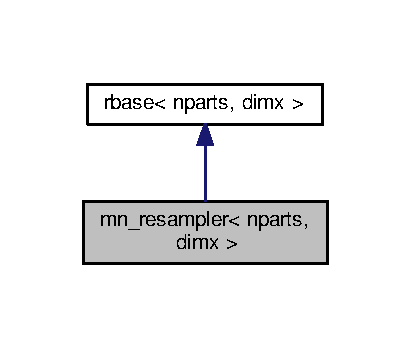
\includegraphics[width=197pt]{classmn__resampler__inherit__graph}
\end{center}
\end{figure}


Collaboration diagram for mn\+\_\+resampler$<$ nparts, dimx, float\+\_\+t $>$\+:\nopagebreak
\begin{figure}[H]
\begin{center}
\leavevmode
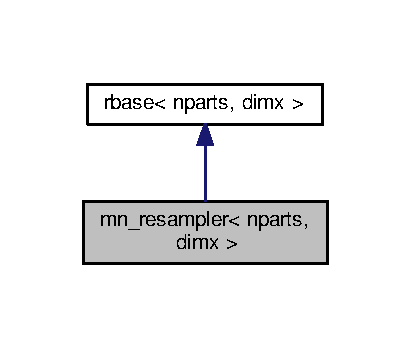
\includegraphics[width=197pt]{classmn__resampler__coll__graph}
\end{center}
\end{figure}
\subsection*{Public Types}
\begin{DoxyCompactItemize}
\item 
using \hyperlink{classmn__resampler_a1cb075b42f73e01de7fc1b27f51bfc4c}{ssv} = Eigen\+::\+Matrix$<$ float\+\_\+t, dimx, 1 $>$
\item 
using \hyperlink{classmn__resampler_aa8ff37576399807b14a7a12615032bb1}{array\+Vec} = std\+::array$<$ \hyperlink{classrbase_ae20e0b8df15aa109252f57ecbf1f20f8}{ssv}, nparts $>$
\item 
using \hyperlink{classmn__resampler_ae26be2889cf3cd4ddea66928d879809e}{array\+Float} = std\+::array$<$ float\+\_\+t, nparts $>$
\item 
using \hyperlink{classmn__resampler_afb5d000e2464afef813792c57c42599b}{array\+Int} = std\+::array$<$ unsigned int, nparts $>$
\end{DoxyCompactItemize}
\subsection*{Public Member Functions}
\begin{DoxyCompactItemize}
\item 
\mbox{\Hypertarget{classmn__resampler_a016a00570c30806a0fdad25385395f95}\label{classmn__resampler_a016a00570c30806a0fdad25385395f95}} 
\hyperlink{classmn__resampler_a016a00570c30806a0fdad25385395f95}{mn\+\_\+resampler} ()=default
\begin{DoxyCompactList}\small\item\em Default constructor. Only option available. \end{DoxyCompactList}\item 
void \hyperlink{classmn__resampler_a13b1897e180a791a3a099d5d6329a125}{resamp\+Log\+Wts} (\hyperlink{classrbase_aa12fc826befa6ba0647b5f59ebc396ee}{array\+Vec} \&old\+Parts, \hyperlink{classrbase_a6f76bef853e508cb5b6f546d231b06f5}{array\+Float} \&old\+Log\+Un\+Norm\+Wts)
\begin{DoxyCompactList}\small\item\em resamples particles. \end{DoxyCompactList}\end{DoxyCompactItemize}
\subsection*{Additional Inherited Members}


\subsection{Detailed Description}
\subsubsection*{template$<$size\+\_\+t nparts, size\+\_\+t dimx, typename float\+\_\+t$>$\newline
class mn\+\_\+resampler$<$ nparts, dimx, float\+\_\+t $>$}

\begin{DoxyAuthor}{Author}
taylor 
\end{DoxyAuthor}
\begin{DoxyDate}{Date}
15/04/18 
\end{DoxyDate}


\subsection{Member Typedef Documentation}
\mbox{\Hypertarget{classmn__resampler_ae26be2889cf3cd4ddea66928d879809e}\label{classmn__resampler_ae26be2889cf3cd4ddea66928d879809e}} 
\index{mn\+\_\+resampler@{mn\+\_\+resampler}!array\+Float@{array\+Float}}
\index{array\+Float@{array\+Float}!mn\+\_\+resampler@{mn\+\_\+resampler}}
\subsubsection{\texorpdfstring{array\+Float}{arrayFloat}}
{\footnotesize\ttfamily template$<$size\+\_\+t nparts, size\+\_\+t dimx, typename float\+\_\+t $>$ \\
using \hyperlink{classmn__resampler}{mn\+\_\+resampler}$<$ nparts, dimx, float\+\_\+t $>$\+::\hyperlink{classrbase_a6f76bef853e508cb5b6f546d231b06f5}{array\+Float} =  std\+::array$<$float\+\_\+t,nparts$>$}

type alias for array of float\+\_\+ts \mbox{\Hypertarget{classmn__resampler_afb5d000e2464afef813792c57c42599b}\label{classmn__resampler_afb5d000e2464afef813792c57c42599b}} 
\index{mn\+\_\+resampler@{mn\+\_\+resampler}!array\+Int@{array\+Int}}
\index{array\+Int@{array\+Int}!mn\+\_\+resampler@{mn\+\_\+resampler}}
\subsubsection{\texorpdfstring{array\+Int}{arrayInt}}
{\footnotesize\ttfamily template$<$size\+\_\+t nparts, size\+\_\+t dimx, typename float\+\_\+t $>$ \\
using \hyperlink{classmn__resampler}{mn\+\_\+resampler}$<$ nparts, dimx, float\+\_\+t $>$\+::\hyperlink{classmn__resampler_afb5d000e2464afef813792c57c42599b}{array\+Int} =  std\+::array$<$unsigned int,nparts$>$}

type alias for array of integers \mbox{\Hypertarget{classmn__resampler_aa8ff37576399807b14a7a12615032bb1}\label{classmn__resampler_aa8ff37576399807b14a7a12615032bb1}} 
\index{mn\+\_\+resampler@{mn\+\_\+resampler}!array\+Vec@{array\+Vec}}
\index{array\+Vec@{array\+Vec}!mn\+\_\+resampler@{mn\+\_\+resampler}}
\subsubsection{\texorpdfstring{array\+Vec}{arrayVec}}
{\footnotesize\ttfamily template$<$size\+\_\+t nparts, size\+\_\+t dimx, typename float\+\_\+t $>$ \\
using \hyperlink{classmn__resampler}{mn\+\_\+resampler}$<$ nparts, dimx, float\+\_\+t $>$\+::\hyperlink{classrbase_aa12fc826befa6ba0647b5f59ebc396ee}{array\+Vec} =  std\+::array$<$\hyperlink{classrbase_ae20e0b8df15aa109252f57ecbf1f20f8}{ssv}, nparts$>$}

type alias for array of Eigen Matrices \mbox{\Hypertarget{classmn__resampler_a1cb075b42f73e01de7fc1b27f51bfc4c}\label{classmn__resampler_a1cb075b42f73e01de7fc1b27f51bfc4c}} 
\index{mn\+\_\+resampler@{mn\+\_\+resampler}!ssv@{ssv}}
\index{ssv@{ssv}!mn\+\_\+resampler@{mn\+\_\+resampler}}
\subsubsection{\texorpdfstring{ssv}{ssv}}
{\footnotesize\ttfamily template$<$size\+\_\+t nparts, size\+\_\+t dimx, typename float\+\_\+t $>$ \\
using \hyperlink{classmn__resampler}{mn\+\_\+resampler}$<$ nparts, dimx, float\+\_\+t $>$\+::\hyperlink{classrbase_ae20e0b8df15aa109252f57ecbf1f20f8}{ssv} =  Eigen\+::\+Matrix$<$float\+\_\+t,dimx,1$>$}

type alias for linear algebra stuff 

\subsection{Member Function Documentation}
\mbox{\Hypertarget{classmn__resampler_a13b1897e180a791a3a099d5d6329a125}\label{classmn__resampler_a13b1897e180a791a3a099d5d6329a125}} 
\index{mn\+\_\+resampler@{mn\+\_\+resampler}!resamp\+Log\+Wts@{resamp\+Log\+Wts}}
\index{resamp\+Log\+Wts@{resamp\+Log\+Wts}!mn\+\_\+resampler@{mn\+\_\+resampler}}
\subsubsection{\texorpdfstring{resamp\+Log\+Wts()}{resampLogWts()}}
{\footnotesize\ttfamily template$<$size\+\_\+t nparts, size\+\_\+t dimx, typename float\+\_\+t $>$ \\
void \hyperlink{classmn__resampler}{mn\+\_\+resampler}$<$ nparts, dimx, float\+\_\+t $>$\+::resamp\+Log\+Wts (\begin{DoxyParamCaption}\item[{\hyperlink{classrbase_aa12fc826befa6ba0647b5f59ebc396ee}{array\+Vec} \&}]{old\+Parts,  }\item[{\hyperlink{classrbase_a6f76bef853e508cb5b6f546d231b06f5}{array\+Float} \&}]{old\+Log\+Un\+Norm\+Wts }\end{DoxyParamCaption})\hspace{0.3cm}{\ttfamily [virtual]}}



resamples particles. 


\begin{DoxyParams}{Parameters}
{\em old\+Parts} & the old particles \\
\hline
{\em old\+Log\+Un\+Norm\+Wts} & the old log unnormalized weights \\
\hline
\end{DoxyParams}


Implements \hyperlink{classrbase_aff0f6f88fd4656e67f5ebc870f10dd44}{rbase$<$ nparts, dimx, float\+\_\+t $>$}.



The documentation for this class was generated from the following file\+:\begin{DoxyCompactItemize}
\item 
include/pf/\hyperlink{resamplers_8h}{resamplers.\+h}\end{DoxyCompactItemize}

\hypertarget{classmn__resampler__rbpf}{}\section{mn\+\_\+resampler\+\_\+rbpf$<$ nparts, dimsampledx, cf\+ModT $>$ Class Template Reference}
\label{classmn__resampler__rbpf}\index{mn\+\_\+resampler\+\_\+rbpf$<$ nparts, dimsampledx, cf\+Mod\+T $>$@{mn\+\_\+resampler\+\_\+rbpf$<$ nparts, dimsampledx, cf\+Mod\+T $>$}}


Performs multinomial resampling for a Rao-\/\+Blackwellized pf.  




{\ttfamily \#include $<$resamplers.\+h$>$}

\subsection*{Public Types}
\begin{DoxyCompactItemize}
\item 
using \hyperlink{classmn__resampler__rbpf_ad5cb01bd12049869984517aa752f6cf6}{ssv} = Eigen\+::\+Matrix$<$ double, dimsampledx, 1 $>$
\item 
using \hyperlink{classmn__resampler__rbpf_ac83764e4eea811b1b76bd2e76de652c9}{array\+Vec} = std\+::array$<$ \hyperlink{classmn__resampler__rbpf_ad5cb01bd12049869984517aa752f6cf6}{ssv}, nparts $>$
\item 
using \hyperlink{classmn__resampler__rbpf_aff8066438dd0932f3ee0602ed1079d3d}{array\+Double} = std\+::array$<$ double, nparts $>$
\item 
using \hyperlink{classmn__resampler__rbpf_adcee7a8490a643233d56f6ba7f1373ee}{array\+Mod} = std\+::array$<$ cf\+ModT, nparts $>$
\end{DoxyCompactItemize}
\subsection*{Public Member Functions}
\begin{DoxyCompactItemize}
\item 
\hyperlink{classmn__resampler__rbpf_a1fad3080bbdbd5f8876a79107774e605}{mn\+\_\+resampler\+\_\+rbpf} ()\hypertarget{classmn__resampler__rbpf_a1fad3080bbdbd5f8876a79107774e605}{}\label{classmn__resampler__rbpf_a1fad3080bbdbd5f8876a79107774e605}

\begin{DoxyCompactList}\small\item\em Default constructor. Only option available. \end{DoxyCompactList}\item 
void \hyperlink{classmn__resampler__rbpf_ae7093100fe2d7c3c91b1764ce724354c}{resamp\+Log\+Wts} (\hyperlink{classmn__resampler__rbpf_adcee7a8490a643233d56f6ba7f1373ee}{array\+Mod} \&old\+Mods, \hyperlink{classmn__resampler__rbpf_ac83764e4eea811b1b76bd2e76de652c9}{array\+Vec} \&old\+Parts, \hyperlink{classmn__resampler__rbpf_aff8066438dd0932f3ee0602ed1079d3d}{array\+Double} \&old\+Log\+Un\+Norm\+Wts)
\begin{DoxyCompactList}\small\item\em resamples particles. \end{DoxyCompactList}\end{DoxyCompactItemize}
\subsection*{Private Attributes}
\begin{DoxyCompactItemize}
\item 
std\+::mt19937 \hyperlink{classmn__resampler__rbpf_a64d1dcb87cc76811719de13160421260}{m\+\_\+gen}\hypertarget{classmn__resampler__rbpf_a64d1dcb87cc76811719de13160421260}{}\label{classmn__resampler__rbpf_a64d1dcb87cc76811719de13160421260}

\begin{DoxyCompactList}\small\item\em prng \end{DoxyCompactList}\end{DoxyCompactItemize}


\subsection{Detailed Description}
\subsubsection*{template$<$size\+\_\+t nparts, size\+\_\+t dimsampledx, typename cf\+ModT$>$\\*
class mn\+\_\+resampler\+\_\+rbpf$<$ nparts, dimsampledx, cf\+Mod\+T $>$}

Performs multinomial resampling for a Rao-\/\+Blackwellized pf. 

\begin{DoxyAuthor}{Author}
taylor 
\end{DoxyAuthor}


\subsection{Member Typedef Documentation}
\index{mn\+\_\+resampler\+\_\+rbpf@{mn\+\_\+resampler\+\_\+rbpf}!array\+Double@{array\+Double}}
\index{array\+Double@{array\+Double}!mn\+\_\+resampler\+\_\+rbpf@{mn\+\_\+resampler\+\_\+rbpf}}
\subsubsection[{\texorpdfstring{array\+Double}{arrayDouble}}]{\setlength{\rightskip}{0pt plus 5cm}template$<$size\+\_\+t nparts, size\+\_\+t dimsampledx, typename cf\+ModT $>$ using {\bf mn\+\_\+resampler\+\_\+rbpf}$<$ nparts, dimsampledx, cf\+ModT $>$\+::{\bf array\+Double} =  std\+::array$<$double,nparts$>$}\hypertarget{classmn__resampler__rbpf_aff8066438dd0932f3ee0602ed1079d3d}{}\label{classmn__resampler__rbpf_aff8066438dd0932f3ee0602ed1079d3d}
type alias for array of doubles \index{mn\+\_\+resampler\+\_\+rbpf@{mn\+\_\+resampler\+\_\+rbpf}!array\+Mod@{array\+Mod}}
\index{array\+Mod@{array\+Mod}!mn\+\_\+resampler\+\_\+rbpf@{mn\+\_\+resampler\+\_\+rbpf}}
\subsubsection[{\texorpdfstring{array\+Mod}{arrayMod}}]{\setlength{\rightskip}{0pt plus 5cm}template$<$size\+\_\+t nparts, size\+\_\+t dimsampledx, typename cf\+ModT $>$ using {\bf mn\+\_\+resampler\+\_\+rbpf}$<$ nparts, dimsampledx, cf\+ModT $>$\+::{\bf array\+Mod} =  std\+::array$<$cf\+ModT,nparts$>$}\hypertarget{classmn__resampler__rbpf_adcee7a8490a643233d56f6ba7f1373ee}{}\label{classmn__resampler__rbpf_adcee7a8490a643233d56f6ba7f1373ee}
type alias for array of closed-\/form models \index{mn\+\_\+resampler\+\_\+rbpf@{mn\+\_\+resampler\+\_\+rbpf}!array\+Vec@{array\+Vec}}
\index{array\+Vec@{array\+Vec}!mn\+\_\+resampler\+\_\+rbpf@{mn\+\_\+resampler\+\_\+rbpf}}
\subsubsection[{\texorpdfstring{array\+Vec}{arrayVec}}]{\setlength{\rightskip}{0pt plus 5cm}template$<$size\+\_\+t nparts, size\+\_\+t dimsampledx, typename cf\+ModT $>$ using {\bf mn\+\_\+resampler\+\_\+rbpf}$<$ nparts, dimsampledx, cf\+ModT $>$\+::{\bf array\+Vec} =  std\+::array$<${\bf ssv}, nparts$>$}\hypertarget{classmn__resampler__rbpf_ac83764e4eea811b1b76bd2e76de652c9}{}\label{classmn__resampler__rbpf_ac83764e4eea811b1b76bd2e76de652c9}
type alias for linear algebra stuff \index{mn\+\_\+resampler\+\_\+rbpf@{mn\+\_\+resampler\+\_\+rbpf}!ssv@{ssv}}
\index{ssv@{ssv}!mn\+\_\+resampler\+\_\+rbpf@{mn\+\_\+resampler\+\_\+rbpf}}
\subsubsection[{\texorpdfstring{ssv}{ssv}}]{\setlength{\rightskip}{0pt plus 5cm}template$<$size\+\_\+t nparts, size\+\_\+t dimsampledx, typename cf\+ModT $>$ using {\bf mn\+\_\+resampler\+\_\+rbpf}$<$ nparts, dimsampledx, cf\+ModT $>$\+::{\bf ssv} =  Eigen\+::\+Matrix$<$double,dimsampledx,1$>$}\hypertarget{classmn__resampler__rbpf_ad5cb01bd12049869984517aa752f6cf6}{}\label{classmn__resampler__rbpf_ad5cb01bd12049869984517aa752f6cf6}
type alias for linear algebra stuff 

\subsection{Member Function Documentation}
\index{mn\+\_\+resampler\+\_\+rbpf@{mn\+\_\+resampler\+\_\+rbpf}!resamp\+Log\+Wts@{resamp\+Log\+Wts}}
\index{resamp\+Log\+Wts@{resamp\+Log\+Wts}!mn\+\_\+resampler\+\_\+rbpf@{mn\+\_\+resampler\+\_\+rbpf}}
\subsubsection[{\texorpdfstring{resamp\+Log\+Wts(array\+Mod \&old\+Mods, array\+Vec \&old\+Parts, array\+Double \&old\+Log\+Un\+Norm\+Wts)}{resampLogWts(arrayMod &oldMods, arrayVec &oldParts, arrayDouble &oldLogUnNormWts)}}]{\setlength{\rightskip}{0pt plus 5cm}template$<$size\+\_\+t nparts, size\+\_\+t dimsampledx, typename cf\+ModT $>$ void {\bf mn\+\_\+resampler\+\_\+rbpf}$<$ nparts, dimsampledx, cf\+ModT $>$\+::resamp\+Log\+Wts (
\begin{DoxyParamCaption}
\item[{{\bf array\+Mod} \&}]{old\+Mods, }
\item[{{\bf array\+Vec} \&}]{old\+Parts, }
\item[{{\bf array\+Double} \&}]{old\+Log\+Un\+Norm\+Wts}
\end{DoxyParamCaption}
)}\hypertarget{classmn__resampler__rbpf_ae7093100fe2d7c3c91b1764ce724354c}{}\label{classmn__resampler__rbpf_ae7093100fe2d7c3c91b1764ce724354c}


resamples particles. 


\begin{DoxyParams}{Parameters}
{\em old\+Mods} & the old closed-\/form models \\
\hline
{\em old\+Parts} & the old particles \\
\hline
{\em old\+Log\+Un\+Norm\+Wts} & the old log unnormalized weights \\
\hline
\end{DoxyParams}


The documentation for this class was generated from the following file\+:\begin{DoxyCompactItemize}
\item 
include/\hyperlink{resamplers_8h}{resamplers.\+h}\end{DoxyCompactItemize}

\hypertarget{classmultivGamFilter}{}\section{multiv\+Gam\+Filter$<$ dim\+\_\+obs, dim\+\_\+pred, float\+\_\+t $>$ Class Template Reference}
\label{classmultivGamFilter}\index{multiv\+Gam\+Filter$<$ dim\+\_\+obs, dim\+\_\+pred, float\+\_\+t $>$@{multiv\+Gam\+Filter$<$ dim\+\_\+obs, dim\+\_\+pred, float\+\_\+t $>$}}


Another class template for Gamma filtering, but this time.  




{\ttfamily \#include $<$cf\+\_\+filters.\+h$>$}



Inheritance diagram for multiv\+Gam\+Filter$<$ dim\+\_\+obs, dim\+\_\+pred, float\+\_\+t $>$\+:\nopagebreak
\begin{figure}[H]
\begin{center}
\leavevmode
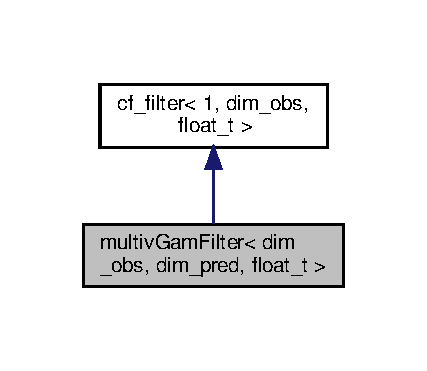
\includegraphics[width=205pt]{classmultivGamFilter__inherit__graph}
\end{center}
\end{figure}


Collaboration diagram for multiv\+Gam\+Filter$<$ dim\+\_\+obs, dim\+\_\+pred, float\+\_\+t $>$\+:\nopagebreak
\begin{figure}[H]
\begin{center}
\leavevmode
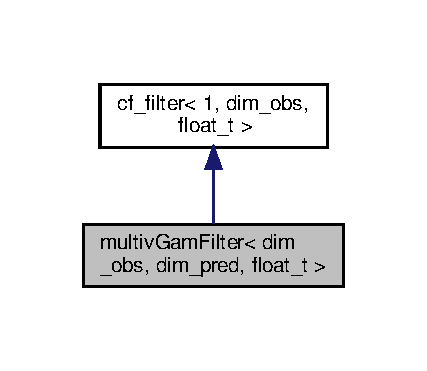
\includegraphics[width=205pt]{classmultivGamFilter__coll__graph}
\end{center}
\end{figure}
\subsection*{Public Types}
\begin{DoxyCompactItemize}
\item 
\mbox{\Hypertarget{classmultivGamFilter_a396935d27512187b9109a70ba04c6abf}\label{classmultivGamFilter_a396935d27512187b9109a70ba04c6abf}} 
using \hyperlink{classmultivGamFilter_a396935d27512187b9109a70ba04c6abf}{psv} = Eigen\+::\+Matrix$<$ float\+\_\+t, dim\+\_\+pred, 1 $>$
\begin{DoxyCompactList}\small\item\em \char`\"{}predictor size vector\char`\"{} \end{DoxyCompactList}\item 
\mbox{\Hypertarget{classmultivGamFilter_a48015c1ef68e2d0a704306b56378417d}\label{classmultivGamFilter_a48015c1ef68e2d0a704306b56378417d}} 
using \hyperlink{classmultivGamFilter_a48015c1ef68e2d0a704306b56378417d}{bsm} = Eigen\+::\+Matrix$<$ float\+\_\+t, dim\+\_\+obs, dim\+\_\+pred $>$
\begin{DoxyCompactList}\small\item\em \char`\"{}beta size matrix\char`\"{} \end{DoxyCompactList}\item 
\mbox{\Hypertarget{classmultivGamFilter_a312ca8e7f1344cdeb01fe9e01850aa8e}\label{classmultivGamFilter_a312ca8e7f1344cdeb01fe9e01850aa8e}} 
using \hyperlink{classmultivGamFilter_a312ca8e7f1344cdeb01fe9e01850aa8e}{tsv} = Eigen\+::\+Matrix$<$ float\+\_\+t, 2, 1 $>$
\begin{DoxyCompactList}\small\item\em \char`\"{}two by 1 vector\char`\"{} to store size and shapes of gamma distributions \end{DoxyCompactList}\item 
\mbox{\Hypertarget{classmultivGamFilter_a34e62f4c6f1de388b86e6106f249cef8}\label{classmultivGamFilter_a34e62f4c6f1de388b86e6106f249cef8}} 
using \hyperlink{classmultivGamFilter_a34e62f4c6f1de388b86e6106f249cef8}{osv} = Eigen\+::\+Matrix$<$ float\+\_\+t, dim\+\_\+obs, 1 $>$
\begin{DoxyCompactList}\small\item\em \char`\"{}observation size vector\char`\"{} \end{DoxyCompactList}\item 
\mbox{\Hypertarget{classmultivGamFilter_af55e5c995ab517331ce05dd7ca4f1781}\label{classmultivGamFilter_af55e5c995ab517331ce05dd7ca4f1781}} 
using \hyperlink{classmultivGamFilter_af55e5c995ab517331ce05dd7ca4f1781}{osm} = Eigen\+::\+Matrix$<$ float\+\_\+t, dim\+\_\+obs, dim\+\_\+obs $>$
\begin{DoxyCompactList}\small\item\em \char`\"{}observation size matrix\char`\"{} \end{DoxyCompactList}\end{DoxyCompactItemize}
\subsection*{Public Member Functions}
\begin{DoxyCompactItemize}
\item 
\hyperlink{classmultivGamFilter_a31e576702f6e72f43744d453b2bc6329}{multiv\+Gam\+Filter} (const float\+\_\+t \&n\+One\+Tilde, const float\+\_\+t \&d\+One\+Tilde)
\begin{DoxyCompactList}\small\item\em Constructor. \end{DoxyCompactList}\item 
\mbox{\Hypertarget{classmultivGamFilter_ad95fbcbba340b6e3e273a9c578bed8e4}\label{classmultivGamFilter_ad95fbcbba340b6e3e273a9c578bed8e4}} 
virtual \hyperlink{classmultivGamFilter_ad95fbcbba340b6e3e273a9c578bed8e4}{$\sim$multiv\+Gam\+Filter} ()
\begin{DoxyCompactList}\small\item\em The (virtual) desuctor. \end{DoxyCompactList}\item 
float\+\_\+t \hyperlink{classmultivGamFilter_ae32c76dd1096041f358962f93de64a99}{get\+Log\+Cond\+Like} () const
\begin{DoxyCompactList}\small\item\em Get the latest conditional likelihood. \end{DoxyCompactList}\item 
\hyperlink{classmultivGamFilter_a312ca8e7f1344cdeb01fe9e01850aa8e}{tsv} \hyperlink{classmultivGamFilter_aaed17907169b5f14a63dbb7b1ed2e1fa}{get\+Filter\+Vec} () const
\begin{DoxyCompactList}\small\item\em Get the current filter vector. \end{DoxyCompactList}\item 
void \hyperlink{classmultivGamFilter_a9e77dfe0fc57ab01005bc054eca37dfa}{update} (const \hyperlink{classmultivGamFilter_a34e62f4c6f1de388b86e6106f249cef8}{osv} \&yt, const \hyperlink{classmultivGamFilter_a396935d27512187b9109a70ba04c6abf}{psv} \&xt, const \hyperlink{classmultivGamFilter_a48015c1ef68e2d0a704306b56378417d}{bsm} \&B, const \hyperlink{classmultivGamFilter_af55e5c995ab517331ce05dd7ca4f1781}{osm} \&Sigma, const float\+\_\+t \&delta)
\begin{DoxyCompactList}\small\item\em Perform a filtering update. \end{DoxyCompactList}\item 
\hyperlink{classmultivGamFilter_a34e62f4c6f1de388b86e6106f249cef8}{osv} \hyperlink{classmultivGamFilter_a6f1387050ad08e7aecececb9cd8eeb71}{get\+Fcast\+Mean} (const \hyperlink{classmultivGamFilter_a396935d27512187b9109a70ba04c6abf}{psv} \&xtp1, const \hyperlink{classmultivGamFilter_a48015c1ef68e2d0a704306b56378417d}{bsm} \&B, const \hyperlink{classmultivGamFilter_af55e5c995ab517331ce05dd7ca4f1781}{osm} \&Sigma, const float\+\_\+t \&delta)
\begin{DoxyCompactList}\small\item\em Get the forecast mean (assuming filtering has been performed already) \end{DoxyCompactList}\item 
\hyperlink{classmultivGamFilter_af55e5c995ab517331ce05dd7ca4f1781}{osm} \hyperlink{classmultivGamFilter_a5cdc2917399fed956b44f69002cae8c3}{get\+Fcast\+Cov} (const \hyperlink{classmultivGamFilter_a396935d27512187b9109a70ba04c6abf}{psv} \&xtp1, const \hyperlink{classmultivGamFilter_a48015c1ef68e2d0a704306b56378417d}{bsm} \&B, const \hyperlink{classmultivGamFilter_af55e5c995ab517331ce05dd7ca4f1781}{osm} \&Sigma, const float\+\_\+t \&delta)
\begin{DoxyCompactList}\small\item\em Get the forecast covariance matrix (assuming filtering has been performed already) \end{DoxyCompactList}\end{DoxyCompactItemize}
\subsection*{Private Attributes}
\begin{DoxyCompactItemize}
\item 
\mbox{\Hypertarget{classmultivGamFilter_a5a0acb67db0bbd0c687c59e3ec05a123}\label{classmultivGamFilter_a5a0acb67db0bbd0c687c59e3ec05a123}} 
\hyperlink{classmultivGamFilter_a312ca8e7f1344cdeb01fe9e01850aa8e}{tsv} \hyperlink{classmultivGamFilter_a5a0acb67db0bbd0c687c59e3ec05a123}{m\+\_\+filt\+Vec}
\begin{DoxyCompactList}\small\item\em filter vector (shape and rate) \end{DoxyCompactList}\item 
\mbox{\Hypertarget{classmultivGamFilter_a0c98ad325dec2868dcc0307f8f438f85}\label{classmultivGamFilter_a0c98ad325dec2868dcc0307f8f438f85}} 
float\+\_\+t \hyperlink{classmultivGamFilter_a0c98ad325dec2868dcc0307f8f438f85}{m\+\_\+last\+Log\+Cond\+Like}
\begin{DoxyCompactList}\small\item\em last log of the conditional likelihood \end{DoxyCompactList}\item 
\mbox{\Hypertarget{classmultivGamFilter_a8ac99863dd918c7fcb6c97a7722efa2b}\label{classmultivGamFilter_a8ac99863dd918c7fcb6c97a7722efa2b}} 
bool \hyperlink{classmultivGamFilter_a8ac99863dd918c7fcb6c97a7722efa2b}{m\+\_\+fresh}
\begin{DoxyCompactList}\small\item\em has data been observed? \end{DoxyCompactList}\end{DoxyCompactItemize}


\subsection{Detailed Description}
\subsubsection*{template$<$size\+\_\+t dim\+\_\+obs, size\+\_\+t dim\+\_\+pred, typename float\+\_\+t$>$\newline
class multiv\+Gam\+Filter$<$ dim\+\_\+obs, dim\+\_\+pred, float\+\_\+t $>$}

Another class template for Gamma filtering, but this time. 

\begin{DoxyAuthor}{Author}
taylor 
\end{DoxyAuthor}


\subsection{Constructor \& Destructor Documentation}
\mbox{\Hypertarget{classmultivGamFilter_a31e576702f6e72f43744d453b2bc6329}\label{classmultivGamFilter_a31e576702f6e72f43744d453b2bc6329}} 
\index{multiv\+Gam\+Filter@{multiv\+Gam\+Filter}!multiv\+Gam\+Filter@{multiv\+Gam\+Filter}}
\index{multiv\+Gam\+Filter@{multiv\+Gam\+Filter}!multiv\+Gam\+Filter@{multiv\+Gam\+Filter}}
\subsubsection{\texorpdfstring{multiv\+Gam\+Filter()}{multivGamFilter()}}
{\footnotesize\ttfamily template$<$size\+\_\+t dim\+\_\+obs, size\+\_\+t dim\+\_\+pred, typename float\+\_\+t $>$ \\
\hyperlink{classmultivGamFilter}{multiv\+Gam\+Filter}$<$ dim\+\_\+obs, dim\+\_\+pred, float\+\_\+t $>$\+::\hyperlink{classmultivGamFilter}{multiv\+Gam\+Filter} (\begin{DoxyParamCaption}\item[{const float\+\_\+t \&}]{n\+One\+Tilde,  }\item[{const float\+\_\+t \&}]{d\+One\+Tilde }\end{DoxyParamCaption})}



Constructor. 


\begin{DoxyParams}{Parameters}
{\em n\+One\+Tilde} & degrees of freedom for time 1 prior. \\
\hline
{\em d\+One\+Tilde} & rate parameter for time 1 prior. \\
\hline
\end{DoxyParams}


\subsection{Member Function Documentation}
\mbox{\Hypertarget{classmultivGamFilter_a5cdc2917399fed956b44f69002cae8c3}\label{classmultivGamFilter_a5cdc2917399fed956b44f69002cae8c3}} 
\index{multiv\+Gam\+Filter@{multiv\+Gam\+Filter}!get\+Fcast\+Cov@{get\+Fcast\+Cov}}
\index{get\+Fcast\+Cov@{get\+Fcast\+Cov}!multiv\+Gam\+Filter@{multiv\+Gam\+Filter}}
\subsubsection{\texorpdfstring{get\+Fcast\+Cov()}{getFcastCov()}}
{\footnotesize\ttfamily template$<$size\+\_\+t dim\+\_\+obs, size\+\_\+t dim\+\_\+pred, typename float\+\_\+t $>$ \\
auto \hyperlink{classmultivGamFilter}{multiv\+Gam\+Filter}$<$ dim\+\_\+obs, dim\+\_\+pred, float\+\_\+t $>$\+::get\+Fcast\+Cov (\begin{DoxyParamCaption}\item[{const \hyperlink{classmultivGamFilter_a396935d27512187b9109a70ba04c6abf}{psv} \&}]{xtp1,  }\item[{const \hyperlink{classmultivGamFilter_a48015c1ef68e2d0a704306b56378417d}{bsm} \&}]{B,  }\item[{const \hyperlink{classmultivGamFilter_af55e5c995ab517331ce05dd7ca4f1781}{osm} \&}]{Sigma,  }\item[{const float\+\_\+t \&}]{delta }\end{DoxyParamCaption})}



Get the forecast covariance matrix (assuming filtering has been performed already) 

gets the forecast covariance matrix! 
\begin{DoxyParams}{Parameters}
{\em xtp1} & the next time period\textquotesingle{}s predictor vector \\
\hline
{\em B} & the loadings matrix \\
\hline
{\em Sigma} & the observation \char`\"{}shape\char`\"{} matrix \\
\hline
{\em delta} & between 0 and 1 the discount parameter \\
\hline
\end{DoxyParams}
\begin{DoxyReturn}{Returns}
a forecast covariance matrix 
\end{DoxyReturn}
\mbox{\Hypertarget{classmultivGamFilter_a6f1387050ad08e7aecececb9cd8eeb71}\label{classmultivGamFilter_a6f1387050ad08e7aecececb9cd8eeb71}} 
\index{multiv\+Gam\+Filter@{multiv\+Gam\+Filter}!get\+Fcast\+Mean@{get\+Fcast\+Mean}}
\index{get\+Fcast\+Mean@{get\+Fcast\+Mean}!multiv\+Gam\+Filter@{multiv\+Gam\+Filter}}
\subsubsection{\texorpdfstring{get\+Fcast\+Mean()}{getFcastMean()}}
{\footnotesize\ttfamily template$<$size\+\_\+t dim\+\_\+obs, size\+\_\+t dim\+\_\+pred, typename float\+\_\+t $>$ \\
auto \hyperlink{classmultivGamFilter}{multiv\+Gam\+Filter}$<$ dim\+\_\+obs, dim\+\_\+pred, float\+\_\+t $>$\+::get\+Fcast\+Mean (\begin{DoxyParamCaption}\item[{const \hyperlink{classmultivGamFilter_a396935d27512187b9109a70ba04c6abf}{psv} \&}]{xtp1,  }\item[{const \hyperlink{classmultivGamFilter_a48015c1ef68e2d0a704306b56378417d}{bsm} \&}]{B,  }\item[{const \hyperlink{classmultivGamFilter_af55e5c995ab517331ce05dd7ca4f1781}{osm} \&}]{Sigma,  }\item[{const float\+\_\+t \&}]{delta }\end{DoxyParamCaption})}



Get the forecast mean (assuming filtering has been performed already) 

gets the forecast mean! 
\begin{DoxyParams}{Parameters}
{\em xtp1} & the next time period\textquotesingle{}s predictor vector \\
\hline
{\em B} & the loadings matrix \\
\hline
{\em Sigma} & the observation \char`\"{}shape\char`\"{} matrix \\
\hline
{\em delta} & between 0 and 1 the discount parameter \\
\hline
\end{DoxyParams}
\begin{DoxyReturn}{Returns}
a mean vector 
\end{DoxyReturn}
\mbox{\Hypertarget{classmultivGamFilter_aaed17907169b5f14a63dbb7b1ed2e1fa}\label{classmultivGamFilter_aaed17907169b5f14a63dbb7b1ed2e1fa}} 
\index{multiv\+Gam\+Filter@{multiv\+Gam\+Filter}!get\+Filter\+Vec@{get\+Filter\+Vec}}
\index{get\+Filter\+Vec@{get\+Filter\+Vec}!multiv\+Gam\+Filter@{multiv\+Gam\+Filter}}
\subsubsection{\texorpdfstring{get\+Filter\+Vec()}{getFilterVec()}}
{\footnotesize\ttfamily template$<$size\+\_\+t dim\+\_\+obs, size\+\_\+t dim\+\_\+pred, typename float\+\_\+t $>$ \\
auto \hyperlink{classmultivGamFilter}{multiv\+Gam\+Filter}$<$ dim\+\_\+obs, dim\+\_\+pred, float\+\_\+t $>$\+::get\+Filter\+Vec (\begin{DoxyParamCaption}{ }\end{DoxyParamCaption}) const}



Get the current filter vector. 

get the current filtering distribution. First element is the shape, second is the rate. \begin{DoxyReturn}{Returns}
a vector of the shape and rate parameters of f(p\+\_\+t $\vert$ y\+\_\+\{1\+:t\}) 
\end{DoxyReturn}
\mbox{\Hypertarget{classmultivGamFilter_ae32c76dd1096041f358962f93de64a99}\label{classmultivGamFilter_ae32c76dd1096041f358962f93de64a99}} 
\index{multiv\+Gam\+Filter@{multiv\+Gam\+Filter}!get\+Log\+Cond\+Like@{get\+Log\+Cond\+Like}}
\index{get\+Log\+Cond\+Like@{get\+Log\+Cond\+Like}!multiv\+Gam\+Filter@{multiv\+Gam\+Filter}}
\subsubsection{\texorpdfstring{get\+Log\+Cond\+Like()}{getLogCondLike()}}
{\footnotesize\ttfamily template$<$size\+\_\+t dim\+\_\+obs, size\+\_\+t dim\+\_\+pred, typename float\+\_\+t $>$ \\
auto \hyperlink{classmultivGamFilter}{multiv\+Gam\+Filter}$<$ dim\+\_\+obs, dim\+\_\+pred, float\+\_\+t $>$\+::get\+Log\+Cond\+Like (\begin{DoxyParamCaption}{ }\end{DoxyParamCaption}) const\hspace{0.3cm}{\ttfamily [virtual]}}



Get the latest conditional likelihood. 

\begin{DoxyReturn}{Returns}
the latest conditional likelihood. 
\end{DoxyReturn}


Implements \hyperlink{classcf__filter_a11b26307172bf94b8075ed2cdb8fc09c}{cf\+\_\+filter$<$ 1, dim\+\_\+obs, float\+\_\+t $>$}.

\mbox{\Hypertarget{classmultivGamFilter_a9e77dfe0fc57ab01005bc054eca37dfa}\label{classmultivGamFilter_a9e77dfe0fc57ab01005bc054eca37dfa}} 
\index{multiv\+Gam\+Filter@{multiv\+Gam\+Filter}!update@{update}}
\index{update@{update}!multiv\+Gam\+Filter@{multiv\+Gam\+Filter}}
\subsubsection{\texorpdfstring{update()}{update()}}
{\footnotesize\ttfamily template$<$size\+\_\+t dim\+\_\+obs, size\+\_\+t dim\+\_\+pred, typename float\+\_\+t $>$ \\
void \hyperlink{classmultivGamFilter}{multiv\+Gam\+Filter}$<$ dim\+\_\+obs, dim\+\_\+pred, float\+\_\+t $>$\+::update (\begin{DoxyParamCaption}\item[{const \hyperlink{classmultivGamFilter_a34e62f4c6f1de388b86e6106f249cef8}{osv} \&}]{yt,  }\item[{const \hyperlink{classmultivGamFilter_a396935d27512187b9109a70ba04c6abf}{psv} \&}]{xt,  }\item[{const \hyperlink{classmultivGamFilter_a48015c1ef68e2d0a704306b56378417d}{bsm} \&}]{B,  }\item[{const \hyperlink{classmultivGamFilter_af55e5c995ab517331ce05dd7ca4f1781}{osm} \&}]{Sigma,  }\item[{const float\+\_\+t \&}]{delta }\end{DoxyParamCaption})}



Perform a filtering update. 

Perform a Gamma filter update. 
\begin{DoxyParams}{Parameters}
{\em yt} & the most recent dependent random variable \\
\hline
{\em xt} & the most recent predictor vector \\
\hline
{\em B} & the loadings matrix \\
\hline
{\em Sigma} & the observation \char`\"{}shape\char`\"{} matrix. \\
\hline
{\em delta} & between 0 and 1 the discount parameter \\
\hline
\end{DoxyParams}


The documentation for this class was generated from the following file\+:\begin{DoxyCompactItemize}
\item 
include/pf/\hyperlink{cf__filters_8h}{cf\+\_\+filters.\+h}\end{DoxyCompactItemize}

\hypertarget{classrvsamp_1_1MVNSampler}{}\section{rvsamp\+:\+:M\+V\+N\+Sampler$<$ dim, float\+\_\+t $>$ Class Template Reference}
\label{classrvsamp_1_1MVNSampler}\index{rvsamp\+::\+M\+V\+N\+Sampler$<$ dim, float\+\_\+t $>$@{rvsamp\+::\+M\+V\+N\+Sampler$<$ dim, float\+\_\+t $>$}}


A class that performs sampling from a multivariate normal distribution.  




{\ttfamily \#include $<$rv\+\_\+samp.\+h$>$}



Inheritance diagram for rvsamp\+:\+:M\+V\+N\+Sampler$<$ dim, float\+\_\+t $>$\+:\nopagebreak
\begin{figure}[H]
\begin{center}
\leavevmode
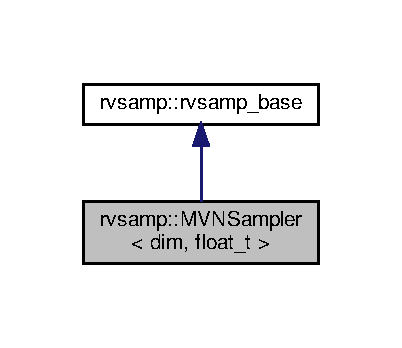
\includegraphics[width=193pt]{classrvsamp_1_1MVNSampler__inherit__graph}
\end{center}
\end{figure}


Collaboration diagram for rvsamp\+:\+:M\+V\+N\+Sampler$<$ dim, float\+\_\+t $>$\+:\nopagebreak
\begin{figure}[H]
\begin{center}
\leavevmode
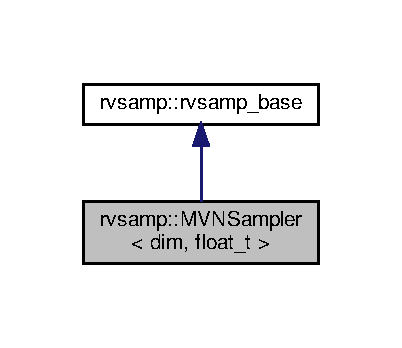
\includegraphics[width=193pt]{classrvsamp_1_1MVNSampler__coll__graph}
\end{center}
\end{figure}
\subsection*{Public Types}
\begin{DoxyCompactItemize}
\item 
using \hyperlink{classrvsamp_1_1MVNSampler_a1110bc1695c5c959914602dbaf2f6878}{Vec} = Eigen\+::\+Matrix$<$ float\+\_\+t, dim, 1 $>$
\item 
using \hyperlink{classrvsamp_1_1MVNSampler_ad6891a72b508fd59263c6d62b6bffd14}{Mat} = Eigen\+::\+Matrix$<$ float\+\_\+t, dim, dim $>$
\end{DoxyCompactItemize}
\subsection*{Public Member Functions}
\begin{DoxyCompactItemize}
\item 
\hyperlink{classrvsamp_1_1MVNSampler_a5fa6029b9bd840c4b08a01f67a97afc6}{M\+V\+N\+Sampler} ()
\begin{DoxyCompactList}\small\item\em Default-\/constructor sets up for multivariate standard Normal random variate generation. \end{DoxyCompactList}\item 
\hyperlink{classrvsamp_1_1MVNSampler_ac41aa5fc1e96bdd0f1577f8382958e7e}{M\+V\+N\+Sampler} (const \hyperlink{classrvsamp_1_1MVNSampler_a1110bc1695c5c959914602dbaf2f6878}{Vec} \&mean\+Vec, const \hyperlink{classrvsamp_1_1MVNSampler_ad6891a72b508fd59263c6d62b6bffd14}{Mat} \&cov\+Mat)
\begin{DoxyCompactList}\small\item\em The user must supply both mean and covariance matrix. \end{DoxyCompactList}\item 
void \hyperlink{classrvsamp_1_1MVNSampler_a9b50fc87640fe9c25595076539cf1c1d}{set\+Covar} (const \hyperlink{classrvsamp_1_1MVNSampler_ad6891a72b508fd59263c6d62b6bffd14}{Mat} \&cov\+Mat)
\begin{DoxyCompactList}\small\item\em sets the covariance matrix of the sampler. \end{DoxyCompactList}\item 
void \hyperlink{classrvsamp_1_1MVNSampler_a99b3bae7eb823d0bfcbbccf89555569e}{set\+Mean} (const \hyperlink{classrvsamp_1_1MVNSampler_a1110bc1695c5c959914602dbaf2f6878}{Vec} \&mean\+Vec)
\begin{DoxyCompactList}\small\item\em sets the mean vector of the sampler. \end{DoxyCompactList}\item 
auto \hyperlink{classrvsamp_1_1MVNSampler_a1b0b148b0d1223e35e317c804c9bf127}{sample} () -\/$>$ \hyperlink{classrvsamp_1_1MVNSampler_a1110bc1695c5c959914602dbaf2f6878}{Vec}
\begin{DoxyCompactList}\small\item\em Draws a random vector. \end{DoxyCompactList}\end{DoxyCompactItemize}
\subsection*{Private Attributes}
\begin{DoxyCompactItemize}
\item 
\mbox{\Hypertarget{classrvsamp_1_1MVNSampler_a44d420b751e226b77d8fdfc5c5bef09d}\label{classrvsamp_1_1MVNSampler_a44d420b751e226b77d8fdfc5c5bef09d}} 
std\+::normal\+\_\+distribution$<$ float\+\_\+t $>$ \hyperlink{classrvsamp_1_1MVNSampler_a44d420b751e226b77d8fdfc5c5bef09d}{m\+\_\+z\+\_\+gen}
\begin{DoxyCompactList}\small\item\em makes normal random variates \end{DoxyCompactList}\item 
\mbox{\Hypertarget{classrvsamp_1_1MVNSampler_a80319ff672cddccd2dc48a447a7dfac3}\label{classrvsamp_1_1MVNSampler_a80319ff672cddccd2dc48a447a7dfac3}} 
\hyperlink{classrvsamp_1_1MVNSampler_ad6891a72b508fd59263c6d62b6bffd14}{Mat} \hyperlink{classrvsamp_1_1MVNSampler_a80319ff672cddccd2dc48a447a7dfac3}{m\+\_\+scale\+\_\+mat}
\begin{DoxyCompactList}\small\item\em covariance matrix \end{DoxyCompactList}\item 
\mbox{\Hypertarget{classrvsamp_1_1MVNSampler_a0a1de8eea2dfa214c5495ccf226aba9c}\label{classrvsamp_1_1MVNSampler_a0a1de8eea2dfa214c5495ccf226aba9c}} 
\hyperlink{classrvsamp_1_1MVNSampler_a1110bc1695c5c959914602dbaf2f6878}{Vec} \hyperlink{classrvsamp_1_1MVNSampler_a0a1de8eea2dfa214c5495ccf226aba9c}{m\+\_\+mean}
\begin{DoxyCompactList}\small\item\em mean vector \end{DoxyCompactList}\end{DoxyCompactItemize}
\subsection*{Additional Inherited Members}


\subsection{Detailed Description}
\subsubsection*{template$<$size\+\_\+t dim, typename float\+\_\+t$>$\newline
class rvsamp\+::\+M\+V\+N\+Sampler$<$ dim, float\+\_\+t $>$}

A class that performs sampling from a multivariate normal distribution. 

\begin{DoxyAuthor}{Author}
taylor 
\end{DoxyAuthor}


\subsection{Member Typedef Documentation}
\mbox{\Hypertarget{classrvsamp_1_1MVNSampler_ad6891a72b508fd59263c6d62b6bffd14}\label{classrvsamp_1_1MVNSampler_ad6891a72b508fd59263c6d62b6bffd14}} 
\index{rvsamp\+::\+M\+V\+N\+Sampler@{rvsamp\+::\+M\+V\+N\+Sampler}!Mat@{Mat}}
\index{Mat@{Mat}!rvsamp\+::\+M\+V\+N\+Sampler@{rvsamp\+::\+M\+V\+N\+Sampler}}
\subsubsection{\texorpdfstring{Mat}{Mat}}
{\footnotesize\ttfamily template$<$size\+\_\+t dim, typename float\+\_\+t $>$ \\
using \hyperlink{classrvsamp_1_1MVNSampler}{rvsamp\+::\+M\+V\+N\+Sampler}$<$ dim, float\+\_\+t $>$\+::\hyperlink{classrvsamp_1_1MVNSampler_ad6891a72b508fd59263c6d62b6bffd14}{Mat} =  Eigen\+::\+Matrix$<$float\+\_\+t,dim,dim$>$}

type alias for linear algebra stuff \mbox{\Hypertarget{classrvsamp_1_1MVNSampler_a1110bc1695c5c959914602dbaf2f6878}\label{classrvsamp_1_1MVNSampler_a1110bc1695c5c959914602dbaf2f6878}} 
\index{rvsamp\+::\+M\+V\+N\+Sampler@{rvsamp\+::\+M\+V\+N\+Sampler}!Vec@{Vec}}
\index{Vec@{Vec}!rvsamp\+::\+M\+V\+N\+Sampler@{rvsamp\+::\+M\+V\+N\+Sampler}}
\subsubsection{\texorpdfstring{Vec}{Vec}}
{\footnotesize\ttfamily template$<$size\+\_\+t dim, typename float\+\_\+t $>$ \\
using \hyperlink{classrvsamp_1_1MVNSampler}{rvsamp\+::\+M\+V\+N\+Sampler}$<$ dim, float\+\_\+t $>$\+::\hyperlink{classrvsamp_1_1MVNSampler_a1110bc1695c5c959914602dbaf2f6878}{Vec} =  Eigen\+::\+Matrix$<$float\+\_\+t,dim,1$>$}

type alias for linear algebra stuff 

\subsection{Constructor \& Destructor Documentation}
\mbox{\Hypertarget{classrvsamp_1_1MVNSampler_a5fa6029b9bd840c4b08a01f67a97afc6}\label{classrvsamp_1_1MVNSampler_a5fa6029b9bd840c4b08a01f67a97afc6}} 
\index{rvsamp\+::\+M\+V\+N\+Sampler@{rvsamp\+::\+M\+V\+N\+Sampler}!M\+V\+N\+Sampler@{M\+V\+N\+Sampler}}
\index{M\+V\+N\+Sampler@{M\+V\+N\+Sampler}!rvsamp\+::\+M\+V\+N\+Sampler@{rvsamp\+::\+M\+V\+N\+Sampler}}
\subsubsection{\texorpdfstring{M\+V\+N\+Sampler()}{MVNSampler()}\hspace{0.1cm}{\footnotesize\ttfamily [1/2]}}
{\footnotesize\ttfamily template$<$size\+\_\+t dim, typename float\+\_\+t $>$ \\
\hyperlink{classrvsamp_1_1MVNSampler}{rvsamp\+::\+M\+V\+N\+Sampler}$<$ dim, float\+\_\+t $>$\+::\hyperlink{classrvsamp_1_1MVNSampler}{M\+V\+N\+Sampler} (\begin{DoxyParamCaption}{ }\end{DoxyParamCaption})}



Default-\/constructor sets up for multivariate standard Normal random variate generation. 

\begin{DoxyRefDesc}{Todo}
\item[\hyperlink{todo__todo000003}{Todo}]\+: implement move semantics \end{DoxyRefDesc}
\mbox{\Hypertarget{classrvsamp_1_1MVNSampler_ac41aa5fc1e96bdd0f1577f8382958e7e}\label{classrvsamp_1_1MVNSampler_ac41aa5fc1e96bdd0f1577f8382958e7e}} 
\index{rvsamp\+::\+M\+V\+N\+Sampler@{rvsamp\+::\+M\+V\+N\+Sampler}!M\+V\+N\+Sampler@{M\+V\+N\+Sampler}}
\index{M\+V\+N\+Sampler@{M\+V\+N\+Sampler}!rvsamp\+::\+M\+V\+N\+Sampler@{rvsamp\+::\+M\+V\+N\+Sampler}}
\subsubsection{\texorpdfstring{M\+V\+N\+Sampler()}{MVNSampler()}\hspace{0.1cm}{\footnotesize\ttfamily [2/2]}}
{\footnotesize\ttfamily template$<$size\+\_\+t dim, typename float\+\_\+t $>$ \\
\hyperlink{classrvsamp_1_1MVNSampler}{rvsamp\+::\+M\+V\+N\+Sampler}$<$ dim, float\+\_\+t $>$\+::\hyperlink{classrvsamp_1_1MVNSampler}{M\+V\+N\+Sampler} (\begin{DoxyParamCaption}\item[{const \hyperlink{classrvsamp_1_1MVNSampler_a1110bc1695c5c959914602dbaf2f6878}{Vec} \&}]{mean\+Vec,  }\item[{const \hyperlink{classrvsamp_1_1MVNSampler_ad6891a72b508fd59263c6d62b6bffd14}{Mat} \&}]{cov\+Mat }\end{DoxyParamCaption})}



The user must supply both mean and covariance matrix. 


\begin{DoxyParams}{Parameters}
{\em mean\+Vec} & a Vec for the mean vector of the sampling distribution. \\
\hline
{\em cov\+Mat} & a Mat representing the covariance matrix of the samples. \\
\hline
\end{DoxyParams}


\subsection{Member Function Documentation}
\mbox{\Hypertarget{classrvsamp_1_1MVNSampler_a1b0b148b0d1223e35e317c804c9bf127}\label{classrvsamp_1_1MVNSampler_a1b0b148b0d1223e35e317c804c9bf127}} 
\index{rvsamp\+::\+M\+V\+N\+Sampler@{rvsamp\+::\+M\+V\+N\+Sampler}!sample@{sample}}
\index{sample@{sample}!rvsamp\+::\+M\+V\+N\+Sampler@{rvsamp\+::\+M\+V\+N\+Sampler}}
\subsubsection{\texorpdfstring{sample()}{sample()}}
{\footnotesize\ttfamily template$<$size\+\_\+t dim, typename float\+\_\+t $>$ \\
auto \hyperlink{classrvsamp_1_1MVNSampler}{rvsamp\+::\+M\+V\+N\+Sampler}$<$ dim, float\+\_\+t $>$\+::sample (\begin{DoxyParamCaption}{ }\end{DoxyParamCaption}) -\/$>$ \hyperlink{classrvsamp_1_1MVNSampler_a1110bc1695c5c959914602dbaf2f6878}{Vec}}



Draws a random vector. 

\begin{DoxyReturn}{Returns}
a Vec random sample. 
\end{DoxyReturn}
\mbox{\Hypertarget{classrvsamp_1_1MVNSampler_a9b50fc87640fe9c25595076539cf1c1d}\label{classrvsamp_1_1MVNSampler_a9b50fc87640fe9c25595076539cf1c1d}} 
\index{rvsamp\+::\+M\+V\+N\+Sampler@{rvsamp\+::\+M\+V\+N\+Sampler}!set\+Covar@{set\+Covar}}
\index{set\+Covar@{set\+Covar}!rvsamp\+::\+M\+V\+N\+Sampler@{rvsamp\+::\+M\+V\+N\+Sampler}}
\subsubsection{\texorpdfstring{set\+Covar()}{setCovar()}}
{\footnotesize\ttfamily template$<$size\+\_\+t dim, typename float\+\_\+t $>$ \\
void \hyperlink{classrvsamp_1_1MVNSampler}{rvsamp\+::\+M\+V\+N\+Sampler}$<$ dim, float\+\_\+t $>$\+::set\+Covar (\begin{DoxyParamCaption}\item[{const \hyperlink{classrvsamp_1_1MVNSampler_ad6891a72b508fd59263c6d62b6bffd14}{Mat} \&}]{cov\+Mat }\end{DoxyParamCaption})}



sets the covariance matrix of the sampler. 


\begin{DoxyParams}{Parameters}
{\em cov\+Mat} & the desired covariance matrix. \\
\hline
\end{DoxyParams}
\mbox{\Hypertarget{classrvsamp_1_1MVNSampler_a99b3bae7eb823d0bfcbbccf89555569e}\label{classrvsamp_1_1MVNSampler_a99b3bae7eb823d0bfcbbccf89555569e}} 
\index{rvsamp\+::\+M\+V\+N\+Sampler@{rvsamp\+::\+M\+V\+N\+Sampler}!set\+Mean@{set\+Mean}}
\index{set\+Mean@{set\+Mean}!rvsamp\+::\+M\+V\+N\+Sampler@{rvsamp\+::\+M\+V\+N\+Sampler}}
\subsubsection{\texorpdfstring{set\+Mean()}{setMean()}}
{\footnotesize\ttfamily template$<$size\+\_\+t dim, typename float\+\_\+t $>$ \\
void \hyperlink{classrvsamp_1_1MVNSampler}{rvsamp\+::\+M\+V\+N\+Sampler}$<$ dim, float\+\_\+t $>$\+::set\+Mean (\begin{DoxyParamCaption}\item[{const \hyperlink{classrvsamp_1_1MVNSampler_a1110bc1695c5c959914602dbaf2f6878}{Vec} \&}]{mean\+Vec }\end{DoxyParamCaption})}



sets the mean vector of the sampler. 


\begin{DoxyParams}{Parameters}
{\em mean\+Vec} & the desired mean vector. \\
\hline
\end{DoxyParams}


The documentation for this class was generated from the following file\+:\begin{DoxyCompactItemize}
\item 
include/\hyperlink{rv__samp_8h}{rv\+\_\+samp.\+h}\end{DoxyCompactItemize}

\hypertarget{classpf__base}{}\section{pf\+\_\+base$<$ float\+\_\+t, dimobs, dimstate $>$ Class Template Reference}
\label{classpf__base}\index{pf\+\_\+base$<$ float\+\_\+t, dimobs, dimstate $>$@{pf\+\_\+base$<$ float\+\_\+t, dimobs, dimstate $>$}}
\subsection*{Public Types}
\begin{DoxyCompactItemize}
\item 
\mbox{\Hypertarget{classpf__base_a5c38fdea8b41026d6c5709be11065f0a}\label{classpf__base_a5c38fdea8b41026d6c5709be11065f0a}} 
using {\bfseries float\+\_\+type} = float\+\_\+t
\item 
\mbox{\Hypertarget{classpf__base_ab468bc1a4c41a4ad7372281a1db7db8b}\label{classpf__base_ab468bc1a4c41a4ad7372281a1db7db8b}} 
using {\bfseries osv} = Eigen\+::\+Matrix$<$ float\+\_\+t, dimobs, 1 $>$
\item 
\mbox{\Hypertarget{classpf__base_add01ddbbba6953260f53d47bae2888d2}\label{classpf__base_add01ddbbba6953260f53d47bae2888d2}} 
using {\bfseries ssv} = Eigen\+::\+Matrix$<$ float\+\_\+t, dimstate, 1 $>$
\item 
\mbox{\Hypertarget{classpf__base_a6b7fbe89aa5e34880ad81a5f48e82a04}\label{classpf__base_a6b7fbe89aa5e34880ad81a5f48e82a04}} 
using {\bfseries Mat} = Eigen\+::\+Matrix$<$ float\+\_\+t, Eigen\+::\+Dynamic, Eigen\+::\+Dynamic $>$
\item 
\mbox{\Hypertarget{classpf__base_ae409bcfbd5e1bc542134c4e9b6dce6c3}\label{classpf__base_ae409bcfbd5e1bc542134c4e9b6dce6c3}} 
using {\bfseries func} = std\+::function$<$ const Mat(const ssv \&)$>$
\item 
\mbox{\Hypertarget{classpf__base_a0c328d66f991393ec0f1a082d5cbf4a6}\label{classpf__base_a0c328d66f991393ec0f1a082d5cbf4a6}} 
using {\bfseries funcs} = std\+::vector$<$ func $>$
\end{DoxyCompactItemize}
\subsection*{Public Member Functions}
\begin{DoxyCompactItemize}
\item 
\mbox{\Hypertarget{classpf__base_aec857789031fd938b7088faa3607707a}\label{classpf__base_aec857789031fd938b7088faa3607707a}} 
virtual void \hyperlink{classpf__base_aec857789031fd938b7088faa3607707a}{filter} (const osv \&data, const funcs \&fs=funcs())=0
\begin{DoxyCompactList}\small\item\em the filtering function that must be defined \end{DoxyCompactList}\item 
\mbox{\Hypertarget{classpf__base_a350df818820d6ab0fd6d413022b7f23b}\label{classpf__base_a350df818820d6ab0fd6d413022b7f23b}} 
virtual float\+\_\+t \hyperlink{classpf__base_a350df818820d6ab0fd6d413022b7f23b}{get\+Log\+Cond\+Like} () const =0
\begin{DoxyCompactList}\small\item\em the getter method that must be defined (for conditional log-\/likelihood) \end{DoxyCompactList}\end{DoxyCompactItemize}
\subsection*{Static Public Attributes}
\begin{DoxyCompactItemize}
\item 
\mbox{\Hypertarget{classpf__base_a6fd0ef79ffb005b72045881875fcacb8}\label{classpf__base_a6fd0ef79ffb005b72045881875fcacb8}} 
static constexpr unsigned int {\bfseries dim\+\_\+obs} = dimobs
\item 
\mbox{\Hypertarget{classpf__base_a0a13a058c19940f56d7f30ed5f910f7f}\label{classpf__base_a0a13a058c19940f56d7f30ed5f910f7f}} 
static constexpr unsigned int {\bfseries dim\+\_\+state} = dimstate
\end{DoxyCompactItemize}


The documentation for this class was generated from the following file\+:\begin{DoxyCompactItemize}
\item 
include/pf/\hyperlink{pf__base_8h}{pf\+\_\+base.\+h}\end{DoxyCompactItemize}

\hypertarget{classrbase}{}\section{rbase$<$ nparts, dimx, float\+\_\+t $>$ Class Template Reference}
\label{classrbase}\index{rbase$<$ nparts, dimx, float\+\_\+t $>$@{rbase$<$ nparts, dimx, float\+\_\+t $>$}}


Base class for all resampler types.  




{\ttfamily \#include $<$resamplers.\+h$>$}



Inheritance diagram for rbase$<$ nparts, dimx, float\+\_\+t $>$\+:
\nopagebreak
\begin{figure}[H]
\begin{center}
\leavevmode
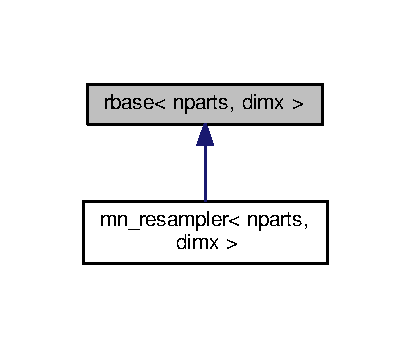
\includegraphics[width=350pt]{classrbase__inherit__graph}
\end{center}
\end{figure}
\subsection*{Public Types}
\begin{DoxyCompactItemize}
\item 
using \hyperlink{classrbase_ae20e0b8df15aa109252f57ecbf1f20f8}{ssv} = Eigen\+::\+Matrix$<$ float\+\_\+t, dimx, 1 $>$
\item 
using \hyperlink{classrbase_aa12fc826befa6ba0647b5f59ebc396ee}{array\+Vec} = std\+::array$<$ \hyperlink{classrbase_ae20e0b8df15aa109252f57ecbf1f20f8}{ssv}, nparts $>$
\item 
using \hyperlink{classrbase_a6f76bef853e508cb5b6f546d231b06f5}{array\+Float} = std\+::array$<$ float\+\_\+t, nparts $>$
\end{DoxyCompactItemize}
\subsection*{Public Member Functions}
\begin{DoxyCompactItemize}
\item 
\mbox{\Hypertarget{classrbase_aae80801bfc60ee3573cb728fc9460b0c}\label{classrbase_aae80801bfc60ee3573cb728fc9460b0c}} 
\hyperlink{classrbase_aae80801bfc60ee3573cb728fc9460b0c}{rbase} ()
\begin{DoxyCompactList}\small\item\em The default constructor gets called by default, and it sets the seed with the clock. \end{DoxyCompactList}\item 
virtual void \hyperlink{classrbase_aff0f6f88fd4656e67f5ebc870f10dd44}{resamp\+Log\+Wts} (\hyperlink{classrbase_aa12fc826befa6ba0647b5f59ebc396ee}{array\+Vec} \&old\+Parts, \hyperlink{classrbase_a6f76bef853e508cb5b6f546d231b06f5}{array\+Float} \&old\+Log\+Un\+Norm\+Wts)=0
\begin{DoxyCompactList}\small\item\em Function to resample from log unnormalized weights. \end{DoxyCompactList}\end{DoxyCompactItemize}
\subsection*{Protected Attributes}
\begin{DoxyCompactItemize}
\item 
\mbox{\Hypertarget{classrbase_ac278c975bd5b23ad009f1ce685552c5c}\label{classrbase_ac278c975bd5b23ad009f1ce685552c5c}} 
std\+::mt19937 \hyperlink{classrbase_ac278c975bd5b23ad009f1ce685552c5c}{m\+\_\+gen}
\begin{DoxyCompactList}\small\item\em prng \end{DoxyCompactList}\end{DoxyCompactItemize}


\subsection{Detailed Description}
\subsubsection*{template$<$size\+\_\+t nparts, size\+\_\+t dimx, typename float\+\_\+t$>$\newline
class rbase$<$ nparts, dimx, float\+\_\+t $>$}

Base class for all resampler types. 

\begin{DoxyAuthor}{Author}
taylor 
\end{DoxyAuthor}
\begin{DoxyDate}{Date}
15/04/18 
\end{DoxyDate}


\subsection{Member Typedef Documentation}
\mbox{\Hypertarget{classrbase_a6f76bef853e508cb5b6f546d231b06f5}\label{classrbase_a6f76bef853e508cb5b6f546d231b06f5}} 
\index{rbase@{rbase}!array\+Float@{array\+Float}}
\index{array\+Float@{array\+Float}!rbase@{rbase}}
\subsubsection{\texorpdfstring{array\+Float}{arrayFloat}}
{\footnotesize\ttfamily template$<$size\+\_\+t nparts, size\+\_\+t dimx, typename float\+\_\+t $>$ \\
using \hyperlink{classrbase}{rbase}$<$ nparts, dimx, float\+\_\+t $>$\+::\hyperlink{classrbase_a6f76bef853e508cb5b6f546d231b06f5}{array\+Float} =  std\+::array$<$float\+\_\+t,nparts$>$}

type alias for array of float\+\_\+ts \mbox{\Hypertarget{classrbase_aa12fc826befa6ba0647b5f59ebc396ee}\label{classrbase_aa12fc826befa6ba0647b5f59ebc396ee}} 
\index{rbase@{rbase}!array\+Vec@{array\+Vec}}
\index{array\+Vec@{array\+Vec}!rbase@{rbase}}
\subsubsection{\texorpdfstring{array\+Vec}{arrayVec}}
{\footnotesize\ttfamily template$<$size\+\_\+t nparts, size\+\_\+t dimx, typename float\+\_\+t $>$ \\
using \hyperlink{classrbase}{rbase}$<$ nparts, dimx, float\+\_\+t $>$\+::\hyperlink{classrbase_aa12fc826befa6ba0647b5f59ebc396ee}{array\+Vec} =  std\+::array$<$\hyperlink{classrbase_ae20e0b8df15aa109252f57ecbf1f20f8}{ssv}, nparts$>$}

type alias for array of Eigen Matrices \mbox{\Hypertarget{classrbase_ae20e0b8df15aa109252f57ecbf1f20f8}\label{classrbase_ae20e0b8df15aa109252f57ecbf1f20f8}} 
\index{rbase@{rbase}!ssv@{ssv}}
\index{ssv@{ssv}!rbase@{rbase}}
\subsubsection{\texorpdfstring{ssv}{ssv}}
{\footnotesize\ttfamily template$<$size\+\_\+t nparts, size\+\_\+t dimx, typename float\+\_\+t $>$ \\
using \hyperlink{classrbase}{rbase}$<$ nparts, dimx, float\+\_\+t $>$\+::\hyperlink{classrbase_ae20e0b8df15aa109252f57ecbf1f20f8}{ssv} =  Eigen\+::\+Matrix$<$float\+\_\+t,dimx,1$>$}

type alias for linear algebra stuff 

\subsection{Member Function Documentation}
\mbox{\Hypertarget{classrbase_aff0f6f88fd4656e67f5ebc870f10dd44}\label{classrbase_aff0f6f88fd4656e67f5ebc870f10dd44}} 
\index{rbase@{rbase}!resamp\+Log\+Wts@{resamp\+Log\+Wts}}
\index{resamp\+Log\+Wts@{resamp\+Log\+Wts}!rbase@{rbase}}
\subsubsection{\texorpdfstring{resamp\+Log\+Wts()}{resampLogWts()}}
{\footnotesize\ttfamily template$<$size\+\_\+t nparts, size\+\_\+t dimx, typename float\+\_\+t $>$ \\
virtual void \hyperlink{classrbase}{rbase}$<$ nparts, dimx, float\+\_\+t $>$\+::resamp\+Log\+Wts (\begin{DoxyParamCaption}\item[{\hyperlink{classrbase_aa12fc826befa6ba0647b5f59ebc396ee}{array\+Vec} \&}]{old\+Parts,  }\item[{\hyperlink{classrbase_a6f76bef853e508cb5b6f546d231b06f5}{array\+Float} \&}]{old\+Log\+Un\+Norm\+Wts }\end{DoxyParamCaption})\hspace{0.3cm}{\ttfamily [pure virtual]}}



Function to resample from log unnormalized weights. 


\begin{DoxyParams}{Parameters}
{\em old\+Parts} & \\
\hline
{\em old\+Log\+Un\+Norm\+Wts} & \\
\hline
\end{DoxyParams}


Implemented in \hyperlink{classmn__resamp__fast1_a398e64faa29bafd345c0258ca90d489c}{mn\+\_\+resamp\+\_\+fast1$<$ nparts, dimx, float\+\_\+t $>$}, \hyperlink{classsystematic__resampler_a9467aec6002043f35f40e9e4857021ed}{systematic\+\_\+resampler$<$ nparts, dimx, float\+\_\+t $>$}, \hyperlink{classstratif__resampler_a2588147563bf3fe598e262cae7e125e6}{stratif\+\_\+resampler$<$ nparts, dimx, float\+\_\+t $>$}, \hyperlink{classresid__resampler_ae6957cd1e080ac4313e6b0bc5ae9aa96}{resid\+\_\+resampler$<$ nparts, dimx, float\+\_\+t $>$}, and \hyperlink{classmn__resampler_a13b1897e180a791a3a099d5d6329a125}{mn\+\_\+resampler$<$ nparts, dimx, float\+\_\+t $>$}.



The documentation for this class was generated from the following file\+:\begin{DoxyCompactItemize}
\item 
include/pf/\hyperlink{resamplers_8h}{resamplers.\+h}\end{DoxyCompactItemize}

\hypertarget{classrbpf__base}{}\section{rbpf\+\_\+base$<$ float\+\_\+t, dim\+\_\+s\+\_\+state, dim\+\_\+ns\+\_\+state, dimobs $>$ Class Template Reference}
\label{classrbpf__base}\index{rbpf\+\_\+base$<$ float\+\_\+t, dim\+\_\+s\+\_\+state, dim\+\_\+ns\+\_\+state, dimobs $>$@{rbpf\+\_\+base$<$ float\+\_\+t, dim\+\_\+s\+\_\+state, dim\+\_\+ns\+\_\+state, dimobs $>$}}
\subsection*{Public Types}
\begin{DoxyCompactItemize}
\item 
\mbox{\Hypertarget{classrbpf__base_a232936f9aba33d2cb3ec0a74d86ff673}\label{classrbpf__base_a232936f9aba33d2cb3ec0a74d86ff673}} 
using {\bfseries osv} = Eigen\+::\+Matrix$<$ float\+\_\+t, dimobs, 1 $>$
\item 
\mbox{\Hypertarget{classrbpf__base_ab2eccf330f9b74a01b4131ebf650fc45}\label{classrbpf__base_ab2eccf330f9b74a01b4131ebf650fc45}} 
using {\bfseries sssv} = Eigen\+::\+Matrix$<$ float\+\_\+t, dim\+\_\+s\+\_\+state, 1 $>$
\item 
\mbox{\Hypertarget{classrbpf__base_af80df010347845efac98659ecf7bb1f2}\label{classrbpf__base_af80df010347845efac98659ecf7bb1f2}} 
using {\bfseries nsssv} = Eigen\+::\+Matrix$<$ float\+\_\+t, dim\+\_\+ns\+\_\+state, 1 $>$
\item 
\mbox{\Hypertarget{classrbpf__base_a195c55dcd55fb4a1a5a08c44603bd683}\label{classrbpf__base_a195c55dcd55fb4a1a5a08c44603bd683}} 
using {\bfseries Mat} = Eigen\+::\+Matrix$<$ float\+\_\+t, Eigen\+::\+Dynamic, Eigen\+::\+Dynamic $>$
\item 
\mbox{\Hypertarget{classrbpf__base_ab97a27bf3704125176265f8cbb1ccb75}\label{classrbpf__base_ab97a27bf3704125176265f8cbb1ccb75}} 
using {\bfseries func} = std\+::function$<$ const Mat(const nsssv \&, const sssv \&)$>$
\item 
\mbox{\Hypertarget{classrbpf__base_a5e2ffe0b6e10136fcac986314664f938}\label{classrbpf__base_a5e2ffe0b6e10136fcac986314664f938}} 
using {\bfseries funcs} = std\+::vector$<$ func $>$
\end{DoxyCompactItemize}
\subsection*{Public Member Functions}
\begin{DoxyCompactItemize}
\item 
\mbox{\Hypertarget{classrbpf__base_afe22a67962a28c83b8568b96f80e9c7b}\label{classrbpf__base_afe22a67962a28c83b8568b96f80e9c7b}} 
virtual void {\bfseries filter} (const osv \&data, const funcs \&fs=funcs())=0
\end{DoxyCompactItemize}


The documentation for this class was generated from the following file\+:\begin{DoxyCompactItemize}
\item 
include/\hyperlink{pf__base_8h}{pf\+\_\+base.\+h}\end{DoxyCompactItemize}

\hypertarget{classrbpf__hmm}{}\section{rbpf\+\_\+hmm$<$ nparts, dimnss, dimss, dimy, resampT $>$ Class Template Reference}
\label{classrbpf__hmm}\index{rbpf\+\_\+hmm$<$ nparts, dimnss, dimss, dimy, resamp\+T $>$@{rbpf\+\_\+hmm$<$ nparts, dimnss, dimss, dimy, resamp\+T $>$}}


Rao-\/\+Blackwellized/\+Marginal Particle Filter with inner H\+M\+Ms.  




{\ttfamily \#include $<$rbpf.\+h$>$}

\subsection*{Public Types}
\begin{DoxyCompactItemize}
\item 
using \hyperlink{classrbpf__hmm_aa7d73e78fca38e3652890c5c3680dee9}{sssv} = Eigen\+::\+Matrix$<$ double, dimss, 1 $>$
\item 
using \hyperlink{classrbpf__hmm_a87376e321cce5bd3211825c509d17440}{nsssv} = Eigen\+::\+Matrix$<$ double, dimss, 1 $>$
\item 
using \hyperlink{classrbpf__hmm_a6ce5868477ec9ad6eaa3b3b23e99e1ae}{osv} = Eigen\+::\+Matrix$<$ double, dimy, 1 $>$
\item 
using \hyperlink{classrbpf__hmm_a24eee6edeb28e16e01b69c2f7eab4e06}{nsss\+Mat} = Eigen\+::\+Matrix$<$ double, dimnss, dimnss $>$
\item 
using \hyperlink{classrbpf__hmm_a5977cfebfd8736d3a54390f5a21d40b2}{Mat} = Eigen\+::\+Matrix$<$ double, Eigen\+::\+Dynamic, Eigen\+::\+Dynamic $>$
\item 
using \hyperlink{classrbpf__hmm_a7a98fa51630fb04d09c3bd73e3e82ba8}{array\+Mod} = std\+::array$<$ \hyperlink{classhmm}{hmm}$<$ dimnss, dimy $>$, nparts $>$
\item 
using \hyperlink{classrbpf__hmm_a9d9a1df8406fa41b2422291768d9c2f4}{array\+Vec} = std\+::array$<$ \hyperlink{classrbpf__hmm_aa7d73e78fca38e3652890c5c3680dee9}{sssv}, nparts $>$
\item 
using \hyperlink{classrbpf__hmm_a678ef06587101ea51bbb5709f08644bd}{array\+Double} = std\+::array$<$ double, nparts $>$
\end{DoxyCompactItemize}
\subsection*{Public Member Functions}
\begin{DoxyCompactItemize}
\item 
\hyperlink{classrbpf__hmm_a1598acef2616514ddd2fed7bfd5d8f20}{rbpf\+\_\+hmm} (const unsigned int \&resamp\+\_\+sched)
\begin{DoxyCompactList}\small\item\em The constructor. \end{DoxyCompactList}\item 
void \hyperlink{classrbpf__hmm_a25bb385ac5975fdbb7f461d600fe9cef}{filter} (const \hyperlink{classrbpf__hmm_a6ce5868477ec9ad6eaa3b3b23e99e1ae}{osv} \&data, const std\+::vector$<$ std\+::function$<$ const \hyperlink{classrbpf__hmm_a5977cfebfd8736d3a54390f5a21d40b2}{Mat}(const \hyperlink{classrbpf__hmm_a87376e321cce5bd3211825c509d17440}{nsssv} \&x1t\+Probs, const \hyperlink{classrbpf__hmm_aa7d73e78fca38e3652890c5c3680dee9}{sssv} \&x2t)$>$ $>$ \&fs=std\+::vector$<$ std\+::function$<$ const \hyperlink{classrbpf__hmm_a5977cfebfd8736d3a54390f5a21d40b2}{Mat}(const \hyperlink{classrbpf__hmm_a87376e321cce5bd3211825c509d17440}{nsssv} \&, const \hyperlink{classrbpf__hmm_aa7d73e78fca38e3652890c5c3680dee9}{sssv} \&)$>$ $>$())
\begin{DoxyCompactList}\small\item\em Filter. \end{DoxyCompactList}\item 
double \hyperlink{classrbpf__hmm_aaceb6993d215769a54ba225252a80a45}{get\+Log\+Cond\+Like} () const 
\begin{DoxyCompactList}\small\item\em Get the latest conditional likelihood. \end{DoxyCompactList}\item 
std\+::vector$<$ \hyperlink{classrbpf__hmm_a5977cfebfd8736d3a54390f5a21d40b2}{Mat} $>$ \hyperlink{classrbpf__hmm_a0e312a41dc41343a0b5bafacd7937372}{get\+Expectations} () const 
\begin{DoxyCompactList}\small\item\em Get vector of expectations. \end{DoxyCompactList}\item 
virtual double \hyperlink{classrbpf__hmm_ad81a38661eddbf87db154e74c20f303e}{log\+Mu\+Ev} (const \hyperlink{classrbpf__hmm_aa7d73e78fca38e3652890c5c3680dee9}{sssv} \&x21)=0
\begin{DoxyCompactList}\small\item\em Evaluates the first time state density. \end{DoxyCompactList}\item 
virtual \hyperlink{classrbpf__hmm_aa7d73e78fca38e3652890c5c3680dee9}{sssv} \hyperlink{classrbpf__hmm_a56cdb973648c438201da1b46493520ba}{q1\+Samp} (const \hyperlink{classrbpf__hmm_a6ce5868477ec9ad6eaa3b3b23e99e1ae}{osv} \&y1)=0
\begin{DoxyCompactList}\small\item\em Sample from the first sampler. \end{DoxyCompactList}\item 
virtual nssv \hyperlink{classrbpf__hmm_a61f7b50c4370455efe05aed91c3c9a16}{init\+H\+M\+M\+Prob\+Vec} (const \hyperlink{classrbpf__hmm_aa7d73e78fca38e3652890c5c3680dee9}{sssv} \&x21)=0
\begin{DoxyCompactList}\small\item\em Provides the initial mean vector for each H\+MM filter object. \end{DoxyCompactList}\item 
virtual \hyperlink{classrbpf__hmm_a24eee6edeb28e16e01b69c2f7eab4e06}{nsss\+Mat} \hyperlink{classrbpf__hmm_a14cd4883cc2edccd6116a965b0d9c660}{init\+H\+M\+M\+Trans\+Mat} (const \hyperlink{classrbpf__hmm_aa7d73e78fca38e3652890c5c3680dee9}{sssv} \&x21)=0
\begin{DoxyCompactList}\small\item\em Provides the transition matrix for each H\+MM filter object. \end{DoxyCompactList}\item 
virtual \hyperlink{classrbpf__hmm_aa7d73e78fca38e3652890c5c3680dee9}{sssv} \hyperlink{classrbpf__hmm_a58696602bfcdb2e7fd198861ce6c09bf}{q\+Samp} (const \hyperlink{classrbpf__hmm_aa7d73e78fca38e3652890c5c3680dee9}{sssv} \&x2tm1, const \hyperlink{classrbpf__hmm_a6ce5868477ec9ad6eaa3b3b23e99e1ae}{osv} \&yt)=0
\begin{DoxyCompactList}\small\item\em Samples the time t second component. \end{DoxyCompactList}\item 
virtual double \hyperlink{classrbpf__hmm_a6e6087560ff5ab4689889bd74be88787}{log\+Q1\+Ev} (const \hyperlink{classrbpf__hmm_aa7d73e78fca38e3652890c5c3680dee9}{sssv} \&x21, const \hyperlink{classrbpf__hmm_a6ce5868477ec9ad6eaa3b3b23e99e1ae}{osv} \&y1)=0
\begin{DoxyCompactList}\small\item\em Evaluates the proposal density of the second state component at time 1. \end{DoxyCompactList}\item 
virtual double \hyperlink{classrbpf__hmm_a2993f99b3985ebff416bef584bcde06e}{log\+F\+Ev} (const \hyperlink{classrbpf__hmm_aa7d73e78fca38e3652890c5c3680dee9}{sssv} \&x2t, const \hyperlink{classrbpf__hmm_aa7d73e78fca38e3652890c5c3680dee9}{sssv} \&x2tm1)=0
\begin{DoxyCompactList}\small\item\em Evaluates the state transition density for the second state component. \end{DoxyCompactList}\item 
virtual double \hyperlink{classrbpf__hmm_a89ba86cdefbb69e3d3b5b1b17b51394f}{log\+Q\+Ev} (const \hyperlink{classrbpf__hmm_aa7d73e78fca38e3652890c5c3680dee9}{sssv} \&x2t, const \hyperlink{classrbpf__hmm_aa7d73e78fca38e3652890c5c3680dee9}{sssv} \&x2tm1, const \hyperlink{classrbpf__hmm_a6ce5868477ec9ad6eaa3b3b23e99e1ae}{osv} \&yt)=0
\begin{DoxyCompactList}\small\item\em Evaluates the proposal density at time t $>$ 1. \end{DoxyCompactList}\item 
virtual void \hyperlink{classrbpf__hmm_a3eaa1683d31020c62901c68264d0ec1c}{update\+H\+MM} (\hyperlink{classhmm}{hmm}$<$ dimnss, dimy $>$ \&a\+Model, const \hyperlink{classrbpf__hmm_a6ce5868477ec9ad6eaa3b3b23e99e1ae}{osv} \&yt, const \hyperlink{classrbpf__hmm_aa7d73e78fca38e3652890c5c3680dee9}{sssv} \&x2t)=0
\begin{DoxyCompactList}\small\item\em How to update your inner H\+MM filter object at each time. \end{DoxyCompactList}\end{DoxyCompactItemize}
\subsection*{Private Attributes}
\begin{DoxyCompactItemize}
\item 
unsigned int \hyperlink{classrbpf__hmm_a4efe6f063d6b2771c37ccb9a15ffa2c1}{m\+\_\+now}
\item 
double \hyperlink{classrbpf__hmm_aa0356c668abebeb05517aa15b641bd3c}{m\+\_\+last\+Log\+Cond\+Like}
\item 
unsigned int \hyperlink{classrbpf__hmm_a9f26da56457265fae51fdc56e8356f68}{m\+\_\+rs}
\item 
\hyperlink{classrbpf__hmm_a7a98fa51630fb04d09c3bd73e3e82ba8}{array\+Mod} \hyperlink{classrbpf__hmm_a8f6bb61b659415364e81c3286e92e180}{m\+\_\+p\+\_\+inner\+Mods}
\item 
\hyperlink{classrbpf__hmm_a9d9a1df8406fa41b2422291768d9c2f4}{array\+Vec} \hyperlink{classrbpf__hmm_ab64da08863b466fb14c0bcb2a2cbec70}{m\+\_\+p\+\_\+samps}
\item 
\hyperlink{classrbpf__hmm_a678ef06587101ea51bbb5709f08644bd}{array\+Double} \hyperlink{classrbpf__hmm_ad39632bbb88e1a1e8bb213343603fe6d}{m\+\_\+log\+Un\+Norm\+Weights}
\item 
resampT \hyperlink{classrbpf__hmm_af89d83ded78477186aab75c045112901}{m\+\_\+resampler}
\item 
std\+::vector$<$ \hyperlink{classrbpf__hmm_a5977cfebfd8736d3a54390f5a21d40b2}{Mat} $>$ \hyperlink{classrbpf__hmm_a659a1dcc02173d94e2c6f6f26639e1db}{m\+\_\+expectations}
\end{DoxyCompactItemize}


\subsection{Detailed Description}
\subsubsection*{template$<$size\+\_\+t nparts, size\+\_\+t dimnss, size\+\_\+t dimss, size\+\_\+t dimy, typename resampT$>$\\*
class rbpf\+\_\+hmm$<$ nparts, dimnss, dimss, dimy, resamp\+T $>$}

Rao-\/\+Blackwellized/\+Marginal Particle Filter with inner H\+M\+Ms. 

\begin{DoxyAuthor}{Author}
t 
\end{DoxyAuthor}


\subsection{Member Typedef Documentation}
\index{rbpf\+\_\+hmm@{rbpf\+\_\+hmm}!array\+Double@{array\+Double}}
\index{array\+Double@{array\+Double}!rbpf\+\_\+hmm@{rbpf\+\_\+hmm}}
\subsubsection[{\texorpdfstring{array\+Double}{arrayDouble}}]{\setlength{\rightskip}{0pt plus 5cm}template$<$size\+\_\+t nparts, size\+\_\+t dimnss, size\+\_\+t dimss, size\+\_\+t dimy, typename resampT $>$ using {\bf rbpf\+\_\+hmm}$<$ nparts, dimnss, dimss, dimy, resampT $>$\+::{\bf array\+Double} =  std\+::array$<$double,nparts$>$}\hypertarget{classrbpf__hmm_a678ef06587101ea51bbb5709f08644bd}{}\label{classrbpf__hmm_a678ef06587101ea51bbb5709f08644bd}
array of weights \index{rbpf\+\_\+hmm@{rbpf\+\_\+hmm}!array\+Mod@{array\+Mod}}
\index{array\+Mod@{array\+Mod}!rbpf\+\_\+hmm@{rbpf\+\_\+hmm}}
\subsubsection[{\texorpdfstring{array\+Mod}{arrayMod}}]{\setlength{\rightskip}{0pt plus 5cm}template$<$size\+\_\+t nparts, size\+\_\+t dimnss, size\+\_\+t dimss, size\+\_\+t dimy, typename resampT $>$ using {\bf rbpf\+\_\+hmm}$<$ nparts, dimnss, dimss, dimy, resampT $>$\+::{\bf array\+Mod} =  std\+::array$<${\bf hmm}$<$dimnss,dimy$>$,nparts$>$}\hypertarget{classrbpf__hmm_a7a98fa51630fb04d09c3bd73e3e82ba8}{}\label{classrbpf__hmm_a7a98fa51630fb04d09c3bd73e3e82ba8}
array of model objects \index{rbpf\+\_\+hmm@{rbpf\+\_\+hmm}!array\+Vec@{array\+Vec}}
\index{array\+Vec@{array\+Vec}!rbpf\+\_\+hmm@{rbpf\+\_\+hmm}}
\subsubsection[{\texorpdfstring{array\+Vec}{arrayVec}}]{\setlength{\rightskip}{0pt plus 5cm}template$<$size\+\_\+t nparts, size\+\_\+t dimnss, size\+\_\+t dimss, size\+\_\+t dimy, typename resampT $>$ using {\bf rbpf\+\_\+hmm}$<$ nparts, dimnss, dimss, dimy, resampT $>$\+::{\bf array\+Vec} =  std\+::array$<${\bf sssv},nparts$>$}\hypertarget{classrbpf__hmm_a9d9a1df8406fa41b2422291768d9c2f4}{}\label{classrbpf__hmm_a9d9a1df8406fa41b2422291768d9c2f4}
array of samples \index{rbpf\+\_\+hmm@{rbpf\+\_\+hmm}!Mat@{Mat}}
\index{Mat@{Mat}!rbpf\+\_\+hmm@{rbpf\+\_\+hmm}}
\subsubsection[{\texorpdfstring{Mat}{Mat}}]{\setlength{\rightskip}{0pt plus 5cm}template$<$size\+\_\+t nparts, size\+\_\+t dimnss, size\+\_\+t dimss, size\+\_\+t dimy, typename resampT $>$ using {\bf rbpf\+\_\+hmm}$<$ nparts, dimnss, dimss, dimy, resampT $>$\+::{\bf Mat} =  Eigen\+::\+Matrix$<$double,Eigen\+::\+Dynamic,Eigen\+::\+Dynamic$>$}\hypertarget{classrbpf__hmm_a5977cfebfd8736d3a54390f5a21d40b2}{}\label{classrbpf__hmm_a5977cfebfd8736d3a54390f5a21d40b2}
Dynamic size matrix \index{rbpf\+\_\+hmm@{rbpf\+\_\+hmm}!nsss\+Mat@{nsss\+Mat}}
\index{nsss\+Mat@{nsss\+Mat}!rbpf\+\_\+hmm@{rbpf\+\_\+hmm}}
\subsubsection[{\texorpdfstring{nsss\+Mat}{nsssMat}}]{\setlength{\rightskip}{0pt plus 5cm}template$<$size\+\_\+t nparts, size\+\_\+t dimnss, size\+\_\+t dimss, size\+\_\+t dimy, typename resampT $>$ using {\bf rbpf\+\_\+hmm}$<$ nparts, dimnss, dimss, dimy, resampT $>$\+::{\bf nsss\+Mat} =  Eigen\+::\+Matrix$<$double,dimnss,dimnss$>$}\hypertarget{classrbpf__hmm_a24eee6edeb28e16e01b69c2f7eab4e06}{}\label{classrbpf__hmm_a24eee6edeb28e16e01b69c2f7eab4e06}
\char`\"{}not sampled state size matrix\char`\"{} \index{rbpf\+\_\+hmm@{rbpf\+\_\+hmm}!nsssv@{nsssv}}
\index{nsssv@{nsssv}!rbpf\+\_\+hmm@{rbpf\+\_\+hmm}}
\subsubsection[{\texorpdfstring{nsssv}{nsssv}}]{\setlength{\rightskip}{0pt plus 5cm}template$<$size\+\_\+t nparts, size\+\_\+t dimnss, size\+\_\+t dimss, size\+\_\+t dimy, typename resampT $>$ using {\bf rbpf\+\_\+hmm}$<$ nparts, dimnss, dimss, dimy, resampT $>$\+::{\bf nsssv} =  Eigen\+::\+Matrix$<$double,dimss,1$>$}\hypertarget{classrbpf__hmm_a87376e321cce5bd3211825c509d17440}{}\label{classrbpf__hmm_a87376e321cce5bd3211825c509d17440}
\char`\"{}not sampled state size vector\char`\"{} \index{rbpf\+\_\+hmm@{rbpf\+\_\+hmm}!osv@{osv}}
\index{osv@{osv}!rbpf\+\_\+hmm@{rbpf\+\_\+hmm}}
\subsubsection[{\texorpdfstring{osv}{osv}}]{\setlength{\rightskip}{0pt plus 5cm}template$<$size\+\_\+t nparts, size\+\_\+t dimnss, size\+\_\+t dimss, size\+\_\+t dimy, typename resampT $>$ using {\bf rbpf\+\_\+hmm}$<$ nparts, dimnss, dimss, dimy, resampT $>$\+::{\bf osv} =  Eigen\+::\+Matrix$<$double,dimy,1$>$}\hypertarget{classrbpf__hmm_a6ce5868477ec9ad6eaa3b3b23e99e1ae}{}\label{classrbpf__hmm_a6ce5868477ec9ad6eaa3b3b23e99e1ae}
\char`\"{}observation size vector\char`\"{} \index{rbpf\+\_\+hmm@{rbpf\+\_\+hmm}!sssv@{sssv}}
\index{sssv@{sssv}!rbpf\+\_\+hmm@{rbpf\+\_\+hmm}}
\subsubsection[{\texorpdfstring{sssv}{sssv}}]{\setlength{\rightskip}{0pt plus 5cm}template$<$size\+\_\+t nparts, size\+\_\+t dimnss, size\+\_\+t dimss, size\+\_\+t dimy, typename resampT $>$ using {\bf rbpf\+\_\+hmm}$<$ nparts, dimnss, dimss, dimy, resampT $>$\+::{\bf sssv} =  Eigen\+::\+Matrix$<$double,dimss,1$>$}\hypertarget{classrbpf__hmm_aa7d73e78fca38e3652890c5c3680dee9}{}\label{classrbpf__hmm_aa7d73e78fca38e3652890c5c3680dee9}
\char`\"{}sampled state size vector\char`\"{} 

\subsection{Constructor \& Destructor Documentation}
\index{rbpf\+\_\+hmm@{rbpf\+\_\+hmm}!rbpf\+\_\+hmm@{rbpf\+\_\+hmm}}
\index{rbpf\+\_\+hmm@{rbpf\+\_\+hmm}!rbpf\+\_\+hmm@{rbpf\+\_\+hmm}}
\subsubsection[{\texorpdfstring{rbpf\+\_\+hmm(const unsigned int \&resamp\+\_\+sched)}{rbpf_hmm(const unsigned int &resamp_sched)}}]{\setlength{\rightskip}{0pt plus 5cm}template$<$size\+\_\+t nparts, size\+\_\+t dimnss, size\+\_\+t dimss, size\+\_\+t dimy, typename resampT $>$ {\bf rbpf\+\_\+hmm}$<$ nparts, dimnss, dimss, dimy, resampT $>$\+::{\bf rbpf\+\_\+hmm} (
\begin{DoxyParamCaption}
\item[{const unsigned int \&}]{resamp\+\_\+sched}
\end{DoxyParamCaption}
)}\hypertarget{classrbpf__hmm_a1598acef2616514ddd2fed7bfd5d8f20}{}\label{classrbpf__hmm_a1598acef2616514ddd2fed7bfd5d8f20}


The constructor. 

constructor. 
\begin{DoxyParams}{Parameters}
{\em resamp\+\_\+sched} & how often to resample (e.\+g. once every resamp\+\_\+sched time periods) \\
\hline
\end{DoxyParams}


\subsection{Member Function Documentation}
\index{rbpf\+\_\+hmm@{rbpf\+\_\+hmm}!filter@{filter}}
\index{filter@{filter}!rbpf\+\_\+hmm@{rbpf\+\_\+hmm}}
\subsubsection[{\texorpdfstring{filter(const osv \&data, const std\+::vector$<$ std\+::function$<$ const Mat(const nsssv \&x1t\+Probs, const sssv \&x2t)$>$ $>$ \&fs=std\+::vector$<$ std\+::function$<$ const Mat(const nsssv \&, const sssv \&)$>$ $>$())}{filter(const osv &data, const std::vector< std::function< const Mat(const nsssv &x1tProbs, const sssv &x2t)> > &fs=std::vector< std::function< const Mat(const nsssv &, const sssv &)> >())}}]{\setlength{\rightskip}{0pt plus 5cm}template$<$size\+\_\+t nparts, size\+\_\+t dimnss, size\+\_\+t dimss, size\+\_\+t dimy, typename resampT $>$ void {\bf rbpf\+\_\+hmm}$<$ nparts, dimnss, dimss, dimy, resampT $>$\+::filter (
\begin{DoxyParamCaption}
\item[{const {\bf osv} \&}]{data, }
\item[{const std\+::vector$<$ std\+::function$<$ const {\bf Mat}(const {\bf nsssv} \&x1t\+Probs, const {\bf sssv} \&x2t)$>$ $>$ \&}]{fs = {\ttfamily std\+:\+:vector$<$std\+:\+:function$<$const~{\bf Mat}(const~{\bf nsssv}\&,~const~{\bf sssv}\&)$>$~$>$()}}
\end{DoxyParamCaption}
)}\hypertarget{classrbpf__hmm_a25bb385ac5975fdbb7f461d600fe9cef}{}\label{classrbpf__hmm_a25bb385ac5975fdbb7f461d600fe9cef}


Filter. 

filters everything based on a new data point. 
\begin{DoxyParams}{Parameters}
{\em data} & the most recent time series observation. \\
\hline
{\em fs} & a vector of functions computing E\mbox{[}h(x\+\_\+1t, x\+\_\+2t$^\wedge$i)$\vert$ x\+\_\+2t$^\wedge$i,y\+\_\+1\+:t\mbox{]} to be averaged to yield E\mbox{[}h(x\+\_\+1t, x\+\_\+2t)$\vert$,y\+\_\+1\+:t\mbox{]}. Will access the probability vector of x\+\_\+1t \\
\hline
\end{DoxyParams}
\index{rbpf\+\_\+hmm@{rbpf\+\_\+hmm}!get\+Expectations@{get\+Expectations}}
\index{get\+Expectations@{get\+Expectations}!rbpf\+\_\+hmm@{rbpf\+\_\+hmm}}
\subsubsection[{\texorpdfstring{get\+Expectations() const }{getExpectations() const }}]{\setlength{\rightskip}{0pt plus 5cm}template$<$size\+\_\+t nparts, size\+\_\+t dimnss, size\+\_\+t dimss, size\+\_\+t dimy, typename resampT $>$ auto {\bf rbpf\+\_\+hmm}$<$ nparts, dimnss, dimss, dimy, resampT $>$\+::get\+Expectations (
\begin{DoxyParamCaption}
{}
\end{DoxyParamCaption}
) const}\hypertarget{classrbpf__hmm_a0e312a41dc41343a0b5bafacd7937372}{}\label{classrbpf__hmm_a0e312a41dc41343a0b5bafacd7937372}


Get vector of expectations. 

\begin{DoxyReturn}{Returns}
vector of expectations 
\end{DoxyReturn}
\index{rbpf\+\_\+hmm@{rbpf\+\_\+hmm}!get\+Log\+Cond\+Like@{get\+Log\+Cond\+Like}}
\index{get\+Log\+Cond\+Like@{get\+Log\+Cond\+Like}!rbpf\+\_\+hmm@{rbpf\+\_\+hmm}}
\subsubsection[{\texorpdfstring{get\+Log\+Cond\+Like() const }{getLogCondLike() const }}]{\setlength{\rightskip}{0pt plus 5cm}template$<$size\+\_\+t nparts, size\+\_\+t dimnss, size\+\_\+t dimss, size\+\_\+t dimy, typename resampT $>$ double {\bf rbpf\+\_\+hmm}$<$ nparts, dimnss, dimss, dimy, resampT $>$\+::get\+Log\+Cond\+Like (
\begin{DoxyParamCaption}
{}
\end{DoxyParamCaption}
) const}\hypertarget{classrbpf__hmm_aaceb6993d215769a54ba225252a80a45}{}\label{classrbpf__hmm_aaceb6993d215769a54ba225252a80a45}


Get the latest conditional likelihood. 

Get the latest conditional likelihood. \begin{DoxyReturn}{Returns}
the latest conditional likelihood. 
\end{DoxyReturn}
\index{rbpf\+\_\+hmm@{rbpf\+\_\+hmm}!init\+H\+M\+M\+Prob\+Vec@{init\+H\+M\+M\+Prob\+Vec}}
\index{init\+H\+M\+M\+Prob\+Vec@{init\+H\+M\+M\+Prob\+Vec}!rbpf\+\_\+hmm@{rbpf\+\_\+hmm}}
\subsubsection[{\texorpdfstring{init\+H\+M\+M\+Prob\+Vec(const sssv \&x21)=0}{initHMMProbVec(const sssv &x21)=0}}]{\setlength{\rightskip}{0pt plus 5cm}template$<$size\+\_\+t nparts, size\+\_\+t dimnss, size\+\_\+t dimss, size\+\_\+t dimy, typename resampT $>$ virtual nssv {\bf rbpf\+\_\+hmm}$<$ nparts, dimnss, dimss, dimy, resampT $>$\+::init\+H\+M\+M\+Prob\+Vec (
\begin{DoxyParamCaption}
\item[{const {\bf sssv} \&}]{x21}
\end{DoxyParamCaption}
)\hspace{0.3cm}{\ttfamily [pure virtual]}}\hypertarget{classrbpf__hmm_a61f7b50c4370455efe05aed91c3c9a16}{}\label{classrbpf__hmm_a61f7b50c4370455efe05aed91c3c9a16}


Provides the initial mean vector for each H\+MM filter object. 

provides the initial probability vector for each H\+MM filter object. 
\begin{DoxyParams}{Parameters}
{\em x21} & the second state componenent at time 1. \\
\hline
\end{DoxyParams}
\begin{DoxyReturn}{Returns}
a Vec representing the probability of each state element. 
\end{DoxyReturn}
\index{rbpf\+\_\+hmm@{rbpf\+\_\+hmm}!init\+H\+M\+M\+Trans\+Mat@{init\+H\+M\+M\+Trans\+Mat}}
\index{init\+H\+M\+M\+Trans\+Mat@{init\+H\+M\+M\+Trans\+Mat}!rbpf\+\_\+hmm@{rbpf\+\_\+hmm}}
\subsubsection[{\texorpdfstring{init\+H\+M\+M\+Trans\+Mat(const sssv \&x21)=0}{initHMMTransMat(const sssv &x21)=0}}]{\setlength{\rightskip}{0pt plus 5cm}template$<$size\+\_\+t nparts, size\+\_\+t dimnss, size\+\_\+t dimss, size\+\_\+t dimy, typename resampT $>$ virtual {\bf nsss\+Mat} {\bf rbpf\+\_\+hmm}$<$ nparts, dimnss, dimss, dimy, resampT $>$\+::init\+H\+M\+M\+Trans\+Mat (
\begin{DoxyParamCaption}
\item[{const {\bf sssv} \&}]{x21}
\end{DoxyParamCaption}
)\hspace{0.3cm}{\ttfamily [pure virtual]}}\hypertarget{classrbpf__hmm_a14cd4883cc2edccd6116a965b0d9c660}{}\label{classrbpf__hmm_a14cd4883cc2edccd6116a965b0d9c660}


Provides the transition matrix for each H\+MM filter object. 

provides the transition matrix for each H\+MM filter object. 
\begin{DoxyParams}{Parameters}
{\em x21} & the second state component at time 1. \\
\hline
\end{DoxyParams}
\begin{DoxyReturn}{Returns}
a transition matrix where element (ij) is the probability of transitioning from state i to state j. 
\end{DoxyReturn}
\index{rbpf\+\_\+hmm@{rbpf\+\_\+hmm}!log\+F\+Ev@{log\+F\+Ev}}
\index{log\+F\+Ev@{log\+F\+Ev}!rbpf\+\_\+hmm@{rbpf\+\_\+hmm}}
\subsubsection[{\texorpdfstring{log\+F\+Ev(const sssv \&x2t, const sssv \&x2tm1)=0}{logFEv(const sssv &x2t, const sssv &x2tm1)=0}}]{\setlength{\rightskip}{0pt plus 5cm}template$<$size\+\_\+t nparts, size\+\_\+t dimnss, size\+\_\+t dimss, size\+\_\+t dimy, typename resampT $>$ virtual double {\bf rbpf\+\_\+hmm}$<$ nparts, dimnss, dimss, dimy, resampT $>$\+::log\+F\+Ev (
\begin{DoxyParamCaption}
\item[{const {\bf sssv} \&}]{x2t, }
\item[{const {\bf sssv} \&}]{x2tm1}
\end{DoxyParamCaption}
)\hspace{0.3cm}{\ttfamily [pure virtual]}}\hypertarget{classrbpf__hmm_a2993f99b3985ebff416bef584bcde06e}{}\label{classrbpf__hmm_a2993f99b3985ebff416bef584bcde06e}


Evaluates the state transition density for the second state component. 

Evaluates the state transition density for the second state component. 
\begin{DoxyParams}{Parameters}
{\em x2t} & the current second state component. \\
\hline
{\em x2tm1} & the previous second state component. \\
\hline
\end{DoxyParams}
\begin{DoxyReturn}{Returns}
a double evaluation. 
\end{DoxyReturn}
\index{rbpf\+\_\+hmm@{rbpf\+\_\+hmm}!log\+Mu\+Ev@{log\+Mu\+Ev}}
\index{log\+Mu\+Ev@{log\+Mu\+Ev}!rbpf\+\_\+hmm@{rbpf\+\_\+hmm}}
\subsubsection[{\texorpdfstring{log\+Mu\+Ev(const sssv \&x21)=0}{logMuEv(const sssv &x21)=0}}]{\setlength{\rightskip}{0pt plus 5cm}template$<$size\+\_\+t nparts, size\+\_\+t dimnss, size\+\_\+t dimss, size\+\_\+t dimy, typename resampT $>$ virtual double {\bf rbpf\+\_\+hmm}$<$ nparts, dimnss, dimss, dimy, resampT $>$\+::log\+Mu\+Ev (
\begin{DoxyParamCaption}
\item[{const {\bf sssv} \&}]{x21}
\end{DoxyParamCaption}
)\hspace{0.3cm}{\ttfamily [pure virtual]}}\hypertarget{classrbpf__hmm_ad81a38661eddbf87db154e74c20f303e}{}\label{classrbpf__hmm_ad81a38661eddbf87db154e74c20f303e}


Evaluates the first time state density. 

evaluates mu. 
\begin{DoxyParams}{Parameters}
{\em x21} & component two at time 1 \\
\hline
\end{DoxyParams}
\begin{DoxyReturn}{Returns}
a double evaluation 
\end{DoxyReturn}
\index{rbpf\+\_\+hmm@{rbpf\+\_\+hmm}!log\+Q1\+Ev@{log\+Q1\+Ev}}
\index{log\+Q1\+Ev@{log\+Q1\+Ev}!rbpf\+\_\+hmm@{rbpf\+\_\+hmm}}
\subsubsection[{\texorpdfstring{log\+Q1\+Ev(const sssv \&x21, const osv \&y1)=0}{logQ1Ev(const sssv &x21, const osv &y1)=0}}]{\setlength{\rightskip}{0pt plus 5cm}template$<$size\+\_\+t nparts, size\+\_\+t dimnss, size\+\_\+t dimss, size\+\_\+t dimy, typename resampT $>$ virtual double {\bf rbpf\+\_\+hmm}$<$ nparts, dimnss, dimss, dimy, resampT $>$\+::log\+Q1\+Ev (
\begin{DoxyParamCaption}
\item[{const {\bf sssv} \&}]{x21, }
\item[{const {\bf osv} \&}]{y1}
\end{DoxyParamCaption}
)\hspace{0.3cm}{\ttfamily [pure virtual]}}\hypertarget{classrbpf__hmm_a6e6087560ff5ab4689889bd74be88787}{}\label{classrbpf__hmm_a6e6087560ff5ab4689889bd74be88787}


Evaluates the proposal density of the second state component at time 1. 

Evaluates the proposal density of the second state component at time 1. 
\begin{DoxyParams}{Parameters}
{\em x21} & the second state component at time 1 you sampled. \\
\hline
{\em y1} & time 1 observation. \\
\hline
\end{DoxyParams}
\begin{DoxyReturn}{Returns}
a double evaluation of the density. 
\end{DoxyReturn}
\index{rbpf\+\_\+hmm@{rbpf\+\_\+hmm}!log\+Q\+Ev@{log\+Q\+Ev}}
\index{log\+Q\+Ev@{log\+Q\+Ev}!rbpf\+\_\+hmm@{rbpf\+\_\+hmm}}
\subsubsection[{\texorpdfstring{log\+Q\+Ev(const sssv \&x2t, const sssv \&x2tm1, const osv \&yt)=0}{logQEv(const sssv &x2t, const sssv &x2tm1, const osv &yt)=0}}]{\setlength{\rightskip}{0pt plus 5cm}template$<$size\+\_\+t nparts, size\+\_\+t dimnss, size\+\_\+t dimss, size\+\_\+t dimy, typename resampT $>$ virtual double {\bf rbpf\+\_\+hmm}$<$ nparts, dimnss, dimss, dimy, resampT $>$\+::log\+Q\+Ev (
\begin{DoxyParamCaption}
\item[{const {\bf sssv} \&}]{x2t, }
\item[{const {\bf sssv} \&}]{x2tm1, }
\item[{const {\bf osv} \&}]{yt}
\end{DoxyParamCaption}
)\hspace{0.3cm}{\ttfamily [pure virtual]}}\hypertarget{classrbpf__hmm_a89ba86cdefbb69e3d3b5b1b17b51394f}{}\label{classrbpf__hmm_a89ba86cdefbb69e3d3b5b1b17b51394f}


Evaluates the proposal density at time t $>$ 1. 

Evaluates the proposal density at time t $>$ 1. 
\begin{DoxyParams}{Parameters}
{\em x2t} & the current second state component. \\
\hline
{\em x2tm1} & the previous second state component. \\
\hline
{\em yt} & the current time series observation. \\
\hline
\end{DoxyParams}
\begin{DoxyReturn}{Returns}
a double evaluation. 
\end{DoxyReturn}
\index{rbpf\+\_\+hmm@{rbpf\+\_\+hmm}!q1\+Samp@{q1\+Samp}}
\index{q1\+Samp@{q1\+Samp}!rbpf\+\_\+hmm@{rbpf\+\_\+hmm}}
\subsubsection[{\texorpdfstring{q1\+Samp(const osv \&y1)=0}{q1Samp(const osv &y1)=0}}]{\setlength{\rightskip}{0pt plus 5cm}template$<$size\+\_\+t nparts, size\+\_\+t dimnss, size\+\_\+t dimss, size\+\_\+t dimy, typename resampT $>$ virtual {\bf sssv} {\bf rbpf\+\_\+hmm}$<$ nparts, dimnss, dimss, dimy, resampT $>$\+::q1\+Samp (
\begin{DoxyParamCaption}
\item[{const {\bf osv} \&}]{y1}
\end{DoxyParamCaption}
)\hspace{0.3cm}{\ttfamily [pure virtual]}}\hypertarget{classrbpf__hmm_a56cdb973648c438201da1b46493520ba}{}\label{classrbpf__hmm_a56cdb973648c438201da1b46493520ba}


Sample from the first sampler. 

samples the second component of the state at time 1. 
\begin{DoxyParams}{Parameters}
{\em y1} & most recent datum. \\
\hline
\end{DoxyParams}
\begin{DoxyReturn}{Returns}
a sssv sample for x21. 
\end{DoxyReturn}
\index{rbpf\+\_\+hmm@{rbpf\+\_\+hmm}!q\+Samp@{q\+Samp}}
\index{q\+Samp@{q\+Samp}!rbpf\+\_\+hmm@{rbpf\+\_\+hmm}}
\subsubsection[{\texorpdfstring{q\+Samp(const sssv \&x2tm1, const osv \&yt)=0}{qSamp(const sssv &x2tm1, const osv &yt)=0}}]{\setlength{\rightskip}{0pt plus 5cm}template$<$size\+\_\+t nparts, size\+\_\+t dimnss, size\+\_\+t dimss, size\+\_\+t dimy, typename resampT $>$ virtual {\bf sssv} {\bf rbpf\+\_\+hmm}$<$ nparts, dimnss, dimss, dimy, resampT $>$\+::q\+Samp (
\begin{DoxyParamCaption}
\item[{const {\bf sssv} \&}]{x2tm1, }
\item[{const {\bf osv} \&}]{yt}
\end{DoxyParamCaption}
)\hspace{0.3cm}{\ttfamily [pure virtual]}}\hypertarget{classrbpf__hmm_a58696602bfcdb2e7fd198861ce6c09bf}{}\label{classrbpf__hmm_a58696602bfcdb2e7fd198861ce6c09bf}


Samples the time t second component. 

Samples the time t second component. 
\begin{DoxyParams}{Parameters}
{\em x2tm1} & the previous time\textquotesingle{}s second state component. \\
\hline
{\em yt} & the current observation. \\
\hline
\end{DoxyParams}
\begin{DoxyReturn}{Returns}
a Vec sample of the second state component at the current time. 
\end{DoxyReturn}
\index{rbpf\+\_\+hmm@{rbpf\+\_\+hmm}!update\+H\+MM@{update\+H\+MM}}
\index{update\+H\+MM@{update\+H\+MM}!rbpf\+\_\+hmm@{rbpf\+\_\+hmm}}
\subsubsection[{\texorpdfstring{update\+H\+M\+M(hmm$<$ dimnss, dimy $>$ \&a\+Model, const osv \&yt, const sssv \&x2t)=0}{updateHMM(hmm< dimnss, dimy > &aModel, const osv &yt, const sssv &x2t)=0}}]{\setlength{\rightskip}{0pt plus 5cm}template$<$size\+\_\+t nparts, size\+\_\+t dimnss, size\+\_\+t dimss, size\+\_\+t dimy, typename resampT $>$ virtual void {\bf rbpf\+\_\+hmm}$<$ nparts, dimnss, dimss, dimy, resampT $>$\+::update\+H\+MM (
\begin{DoxyParamCaption}
\item[{{\bf hmm}$<$ dimnss, dimy $>$ \&}]{a\+Model, }
\item[{const {\bf osv} \&}]{yt, }
\item[{const {\bf sssv} \&}]{x2t}
\end{DoxyParamCaption}
)\hspace{0.3cm}{\ttfamily [pure virtual]}}\hypertarget{classrbpf__hmm_a3eaa1683d31020c62901c68264d0ec1c}{}\label{classrbpf__hmm_a3eaa1683d31020c62901c68264d0ec1c}


How to update your inner H\+MM filter object at each time. 

How to update your inner H\+MM filter object at each time. 
\begin{DoxyParams}{Parameters}
{\em a\+Model} & a H\+MM filter object describing the conditional closed-\/form model. \\
\hline
{\em yt} & the current time series observation. \\
\hline
{\em x2t} & the current second state component. \\
\hline
\end{DoxyParams}


\subsection{Member Data Documentation}
\index{rbpf\+\_\+hmm@{rbpf\+\_\+hmm}!m\+\_\+expectations@{m\+\_\+expectations}}
\index{m\+\_\+expectations@{m\+\_\+expectations}!rbpf\+\_\+hmm@{rbpf\+\_\+hmm}}
\subsubsection[{\texorpdfstring{m\+\_\+expectations}{m_expectations}}]{\setlength{\rightskip}{0pt plus 5cm}template$<$size\+\_\+t nparts, size\+\_\+t dimnss, size\+\_\+t dimss, size\+\_\+t dimy, typename resampT $>$ std\+::vector$<${\bf Mat}$>$ {\bf rbpf\+\_\+hmm}$<$ nparts, dimnss, dimss, dimy, resampT $>$\+::m\+\_\+expectations\hspace{0.3cm}{\ttfamily [private]}}\hypertarget{classrbpf__hmm_a659a1dcc02173d94e2c6f6f26639e1db}{}\label{classrbpf__hmm_a659a1dcc02173d94e2c6f6f26639e1db}
the vector of expectations \index{rbpf\+\_\+hmm@{rbpf\+\_\+hmm}!m\+\_\+last\+Log\+Cond\+Like@{m\+\_\+last\+Log\+Cond\+Like}}
\index{m\+\_\+last\+Log\+Cond\+Like@{m\+\_\+last\+Log\+Cond\+Like}!rbpf\+\_\+hmm@{rbpf\+\_\+hmm}}
\subsubsection[{\texorpdfstring{m\+\_\+last\+Log\+Cond\+Like}{m_lastLogCondLike}}]{\setlength{\rightskip}{0pt plus 5cm}template$<$size\+\_\+t nparts, size\+\_\+t dimnss, size\+\_\+t dimss, size\+\_\+t dimy, typename resampT $>$ double {\bf rbpf\+\_\+hmm}$<$ nparts, dimnss, dimss, dimy, resampT $>$\+::m\+\_\+last\+Log\+Cond\+Like\hspace{0.3cm}{\ttfamily [private]}}\hypertarget{classrbpf__hmm_aa0356c668abebeb05517aa15b641bd3c}{}\label{classrbpf__hmm_aa0356c668abebeb05517aa15b641bd3c}
last conditional likelihood \index{rbpf\+\_\+hmm@{rbpf\+\_\+hmm}!m\+\_\+log\+Un\+Norm\+Weights@{m\+\_\+log\+Un\+Norm\+Weights}}
\index{m\+\_\+log\+Un\+Norm\+Weights@{m\+\_\+log\+Un\+Norm\+Weights}!rbpf\+\_\+hmm@{rbpf\+\_\+hmm}}
\subsubsection[{\texorpdfstring{m\+\_\+log\+Un\+Norm\+Weights}{m_logUnNormWeights}}]{\setlength{\rightskip}{0pt plus 5cm}template$<$size\+\_\+t nparts, size\+\_\+t dimnss, size\+\_\+t dimss, size\+\_\+t dimy, typename resampT $>$ {\bf array\+Double} {\bf rbpf\+\_\+hmm}$<$ nparts, dimnss, dimss, dimy, resampT $>$\+::m\+\_\+log\+Un\+Norm\+Weights\hspace{0.3cm}{\ttfamily [private]}}\hypertarget{classrbpf__hmm_ad39632bbb88e1a1e8bb213343603fe6d}{}\label{classrbpf__hmm_ad39632bbb88e1a1e8bb213343603fe6d}
the array of unnormalized log-\/weights \index{rbpf\+\_\+hmm@{rbpf\+\_\+hmm}!m\+\_\+now@{m\+\_\+now}}
\index{m\+\_\+now@{m\+\_\+now}!rbpf\+\_\+hmm@{rbpf\+\_\+hmm}}
\subsubsection[{\texorpdfstring{m\+\_\+now}{m_now}}]{\setlength{\rightskip}{0pt plus 5cm}template$<$size\+\_\+t nparts, size\+\_\+t dimnss, size\+\_\+t dimss, size\+\_\+t dimy, typename resampT $>$ unsigned int {\bf rbpf\+\_\+hmm}$<$ nparts, dimnss, dimss, dimy, resampT $>$\+::m\+\_\+now\hspace{0.3cm}{\ttfamily [private]}}\hypertarget{classrbpf__hmm_a4efe6f063d6b2771c37ccb9a15ffa2c1}{}\label{classrbpf__hmm_a4efe6f063d6b2771c37ccb9a15ffa2c1}
the current time period \index{rbpf\+\_\+hmm@{rbpf\+\_\+hmm}!m\+\_\+p\+\_\+inner\+Mods@{m\+\_\+p\+\_\+inner\+Mods}}
\index{m\+\_\+p\+\_\+inner\+Mods@{m\+\_\+p\+\_\+inner\+Mods}!rbpf\+\_\+hmm@{rbpf\+\_\+hmm}}
\subsubsection[{\texorpdfstring{m\+\_\+p\+\_\+inner\+Mods}{m_p_innerMods}}]{\setlength{\rightskip}{0pt plus 5cm}template$<$size\+\_\+t nparts, size\+\_\+t dimnss, size\+\_\+t dimss, size\+\_\+t dimy, typename resampT $>$ {\bf array\+Mod} {\bf rbpf\+\_\+hmm}$<$ nparts, dimnss, dimss, dimy, resampT $>$\+::m\+\_\+p\+\_\+inner\+Mods\hspace{0.3cm}{\ttfamily [private]}}\hypertarget{classrbpf__hmm_a8f6bb61b659415364e81c3286e92e180}{}\label{classrbpf__hmm_a8f6bb61b659415364e81c3286e92e180}
the array of inner closed-\/form models \index{rbpf\+\_\+hmm@{rbpf\+\_\+hmm}!m\+\_\+p\+\_\+samps@{m\+\_\+p\+\_\+samps}}
\index{m\+\_\+p\+\_\+samps@{m\+\_\+p\+\_\+samps}!rbpf\+\_\+hmm@{rbpf\+\_\+hmm}}
\subsubsection[{\texorpdfstring{m\+\_\+p\+\_\+samps}{m_p_samps}}]{\setlength{\rightskip}{0pt plus 5cm}template$<$size\+\_\+t nparts, size\+\_\+t dimnss, size\+\_\+t dimss, size\+\_\+t dimy, typename resampT $>$ {\bf array\+Vec} {\bf rbpf\+\_\+hmm}$<$ nparts, dimnss, dimss, dimy, resampT $>$\+::m\+\_\+p\+\_\+samps\hspace{0.3cm}{\ttfamily [private]}}\hypertarget{classrbpf__hmm_ab64da08863b466fb14c0bcb2a2cbec70}{}\label{classrbpf__hmm_ab64da08863b466fb14c0bcb2a2cbec70}
the array of samples for the second state portion \index{rbpf\+\_\+hmm@{rbpf\+\_\+hmm}!m\+\_\+resampler@{m\+\_\+resampler}}
\index{m\+\_\+resampler@{m\+\_\+resampler}!rbpf\+\_\+hmm@{rbpf\+\_\+hmm}}
\subsubsection[{\texorpdfstring{m\+\_\+resampler}{m_resampler}}]{\setlength{\rightskip}{0pt plus 5cm}template$<$size\+\_\+t nparts, size\+\_\+t dimnss, size\+\_\+t dimss, size\+\_\+t dimy, typename resampT $>$ resampT {\bf rbpf\+\_\+hmm}$<$ nparts, dimnss, dimss, dimy, resampT $>$\+::m\+\_\+resampler\hspace{0.3cm}{\ttfamily [private]}}\hypertarget{classrbpf__hmm_af89d83ded78477186aab75c045112901}{}\label{classrbpf__hmm_af89d83ded78477186aab75c045112901}
the resampler object \index{rbpf\+\_\+hmm@{rbpf\+\_\+hmm}!m\+\_\+rs@{m\+\_\+rs}}
\index{m\+\_\+rs@{m\+\_\+rs}!rbpf\+\_\+hmm@{rbpf\+\_\+hmm}}
\subsubsection[{\texorpdfstring{m\+\_\+rs}{m_rs}}]{\setlength{\rightskip}{0pt plus 5cm}template$<$size\+\_\+t nparts, size\+\_\+t dimnss, size\+\_\+t dimss, size\+\_\+t dimy, typename resampT $>$ unsigned int {\bf rbpf\+\_\+hmm}$<$ nparts, dimnss, dimss, dimy, resampT $>$\+::m\+\_\+rs\hspace{0.3cm}{\ttfamily [private]}}\hypertarget{classrbpf__hmm_a9f26da56457265fae51fdc56e8356f68}{}\label{classrbpf__hmm_a9f26da56457265fae51fdc56e8356f68}
resampling schedue 

The documentation for this class was generated from the following file\+:\begin{DoxyCompactItemize}
\item 
include/\hyperlink{rbpf_8h}{rbpf.\+h}\end{DoxyCompactItemize}

\hypertarget{classrbpf__hmm__bs}{}\section{rbpf\+\_\+hmm\+\_\+bs$<$ nparts, dimnss, dimss, dimy, resampT $>$ Class Template Reference}
\label{classrbpf__hmm__bs}\index{rbpf\+\_\+hmm\+\_\+bs$<$ nparts, dimnss, dimss, dimy, resamp\+T $>$@{rbpf\+\_\+hmm\+\_\+bs$<$ nparts, dimnss, dimss, dimy, resamp\+T $>$}}


Rao-\/\+Blackwellized/\+Marginal Bootstrap Filter with inner H\+M\+Ms.  




{\ttfamily \#include $<$rbpf.\+h$>$}

\subsection*{Public Types}
\begin{DoxyCompactItemize}
\item 
using \hyperlink{classrbpf__hmm__bs_aba47e4a45bf4ac6913f4419f9512f97f}{sssv} = Eigen\+::\+Matrix$<$ double, dimss, 1 $>$
\item 
using \hyperlink{classrbpf__hmm__bs_ad348eec8ba6e192775ff7a7b4a288809}{nsssv} = Eigen\+::\+Matrix$<$ double, dimss, 1 $>$
\item 
using \hyperlink{classrbpf__hmm__bs_a9a830ec4bbd37d4922011165aa5a8037}{osv} = Eigen\+::\+Matrix$<$ double, dimy, 1 $>$
\item 
using \hyperlink{classrbpf__hmm__bs_a1bd1ebb6af375d962ba266b4ed5434a1}{nsss\+Mat} = Eigen\+::\+Matrix$<$ double, dimnss, dimnss $>$
\item 
using \hyperlink{classrbpf__hmm__bs_a8f6996a1394c31ac65859de96f195f3a}{Mat} = Eigen\+::\+Matrix$<$ double, Eigen\+::\+Dynamic, Eigen\+::\+Dynamic $>$
\item 
using \hyperlink{classrbpf__hmm__bs_a9772cd625f6a416ccd54558108b1d7a3}{array\+Mod} = std\+::array$<$ \hyperlink{classhmm}{hmm}$<$ dimnss, dimy $>$, nparts $>$
\item 
using \hyperlink{classrbpf__hmm__bs_a18441e40d4353bf4b91e6cbac001a28b}{array\+Vec} = std\+::array$<$ \hyperlink{classrbpf__hmm__bs_aba47e4a45bf4ac6913f4419f9512f97f}{sssv}, nparts $>$
\item 
using \hyperlink{classrbpf__hmm__bs_a97b5eab2c1fc8acffbdb8941432e8c00}{array\+Double} = std\+::array$<$ double, nparts $>$
\end{DoxyCompactItemize}
\subsection*{Public Member Functions}
\begin{DoxyCompactItemize}
\item 
\hyperlink{classrbpf__hmm__bs_aee5c10d320f7c4d2cf2a3f230fca4f18}{rbpf\+\_\+hmm\+\_\+bs} (const unsigned int \&resamp\+\_\+sched)
\begin{DoxyCompactList}\small\item\em The constructor. \end{DoxyCompactList}\item 
void \hyperlink{classrbpf__hmm__bs_ab04815be8324ccd196427ca95ddf2476}{filter} (const \hyperlink{classrbpf__hmm__bs_a9a830ec4bbd37d4922011165aa5a8037}{osv} \&data, const std\+::vector$<$ std\+::function$<$ const \hyperlink{classrbpf__hmm__bs_a8f6996a1394c31ac65859de96f195f3a}{Mat}(const \hyperlink{classrbpf__hmm__bs_ad348eec8ba6e192775ff7a7b4a288809}{nsssv} \&x1t\+Probs, const \hyperlink{classrbpf__hmm__bs_aba47e4a45bf4ac6913f4419f9512f97f}{sssv} \&x2t)$>$ $>$ \&fs=std\+::vector$<$ std\+::function$<$ const \hyperlink{classrbpf__hmm__bs_a8f6996a1394c31ac65859de96f195f3a}{Mat}(const \hyperlink{classrbpf__hmm__bs_ad348eec8ba6e192775ff7a7b4a288809}{nsssv} \&, const \hyperlink{classrbpf__hmm__bs_aba47e4a45bf4ac6913f4419f9512f97f}{sssv} \&)$>$ $>$())
\begin{DoxyCompactList}\small\item\em Filter. \end{DoxyCompactList}\item 
double \hyperlink{classrbpf__hmm__bs_a0c66c15cb50c5fcd35e68f05092a66f0}{get\+Log\+Cond\+Like} () const 
\begin{DoxyCompactList}\small\item\em Get the latest conditional likelihood. \end{DoxyCompactList}\item 
std\+::vector$<$ \hyperlink{classrbpf__hmm__bs_a8f6996a1394c31ac65859de96f195f3a}{Mat} $>$ \hyperlink{classrbpf__hmm__bs_a4ce1bdcfdebab7410594b8d556444e00}{get\+Expectations} () const 
\begin{DoxyCompactList}\small\item\em Get vector of expectations. \end{DoxyCompactList}\item 
virtual \hyperlink{classrbpf__hmm__bs_aba47e4a45bf4ac6913f4419f9512f97f}{sssv} \hyperlink{classrbpf__hmm__bs_a355305cfff93ccaaccf795481721ab6f}{mu\+Samp} ()=0
\begin{DoxyCompactList}\small\item\em Sample from the first sampler. \end{DoxyCompactList}\item 
virtual nssv \hyperlink{classrbpf__hmm__bs_a01e930554f9a7d847dbe2be4c49db4db}{init\+H\+M\+M\+Prob\+Vec} (const \hyperlink{classrbpf__hmm__bs_aba47e4a45bf4ac6913f4419f9512f97f}{sssv} \&x21)=0
\begin{DoxyCompactList}\small\item\em Provides the initial mean vector for each H\+MM filter object. \end{DoxyCompactList}\item 
virtual \hyperlink{classrbpf__hmm__bs_a1bd1ebb6af375d962ba266b4ed5434a1}{nsss\+Mat} \hyperlink{classrbpf__hmm__bs_a74f41ca3dae17f4dc1962fb61b489038}{init\+H\+M\+M\+Trans\+Mat} (const \hyperlink{classrbpf__hmm__bs_aba47e4a45bf4ac6913f4419f9512f97f}{sssv} \&x21)=0
\begin{DoxyCompactList}\small\item\em Provides the transition matrix for each H\+MM filter object. \end{DoxyCompactList}\item 
virtual \hyperlink{classrbpf__hmm__bs_aba47e4a45bf4ac6913f4419f9512f97f}{sssv} \hyperlink{classrbpf__hmm__bs_a2edca3ded3bbb34f67303f5cc9e40170}{f\+Samp} (const \hyperlink{classrbpf__hmm__bs_aba47e4a45bf4ac6913f4419f9512f97f}{sssv} \&x2tm1)=0
\begin{DoxyCompactList}\small\item\em Samples the time t second component. \end{DoxyCompactList}\item 
virtual void \hyperlink{classrbpf__hmm__bs_ae183b5747ec63cd61031e8bbbfe5fb82}{update\+H\+MM} (\hyperlink{classhmm}{hmm}$<$ dimnss, dimy $>$ \&a\+Model, const \hyperlink{classrbpf__hmm__bs_a9a830ec4bbd37d4922011165aa5a8037}{osv} \&yt, const \hyperlink{classrbpf__hmm__bs_aba47e4a45bf4ac6913f4419f9512f97f}{sssv} \&x2t)=0
\begin{DoxyCompactList}\small\item\em How to update your inner H\+MM filter object at each time. \end{DoxyCompactList}\end{DoxyCompactItemize}
\subsection*{Private Attributes}
\begin{DoxyCompactItemize}
\item 
unsigned int \hyperlink{classrbpf__hmm__bs_ae0102fba0fb6873f0d01ef873fe8dbb1}{m\+\_\+now}
\item 
double \hyperlink{classrbpf__hmm__bs_a84b69c77970140adb2affbdc800e76cc}{m\+\_\+last\+Log\+Cond\+Like}
\item 
unsigned int \hyperlink{classrbpf__hmm__bs_a0b81a949e21d9c1f3c1dcb5c6c4840e2}{m\+\_\+rs}
\item 
\hyperlink{classrbpf__hmm__bs_a9772cd625f6a416ccd54558108b1d7a3}{array\+Mod} \hyperlink{classrbpf__hmm__bs_a66e06e277278568dd484b36065ad38ee}{m\+\_\+p\+\_\+inner\+Mods}
\item 
\hyperlink{classrbpf__hmm__bs_a18441e40d4353bf4b91e6cbac001a28b}{array\+Vec} \hyperlink{classrbpf__hmm__bs_a51c48b58b2be3a82a61fed0f1a44f06d}{m\+\_\+p\+\_\+samps}
\item 
\hyperlink{classrbpf__hmm__bs_a97b5eab2c1fc8acffbdb8941432e8c00}{array\+Double} \hyperlink{classrbpf__hmm__bs_a6a4c6cd6a2ac836dd74d475560aa4048}{m\+\_\+log\+Un\+Norm\+Weights}
\item 
resampT \hyperlink{classrbpf__hmm__bs_a164a9d81ede5be6a9ca0dd33cdffb3c0}{m\+\_\+resampler}
\item 
std\+::vector$<$ \hyperlink{classrbpf__hmm__bs_a8f6996a1394c31ac65859de96f195f3a}{Mat} $>$ \hyperlink{classrbpf__hmm__bs_ac6ab8e527331e321da58501e4a4da14e}{m\+\_\+expectations}
\end{DoxyCompactItemize}


\subsection{Detailed Description}
\subsubsection*{template$<$size\+\_\+t nparts, size\+\_\+t dimnss, size\+\_\+t dimss, size\+\_\+t dimy, typename resampT$>$\\*
class rbpf\+\_\+hmm\+\_\+bs$<$ nparts, dimnss, dimss, dimy, resamp\+T $>$}

Rao-\/\+Blackwellized/\+Marginal Bootstrap Filter with inner H\+M\+Ms. 

\begin{DoxyAuthor}{Author}
t 
\end{DoxyAuthor}


\subsection{Member Typedef Documentation}
\index{rbpf\+\_\+hmm\+\_\+bs@{rbpf\+\_\+hmm\+\_\+bs}!array\+Double@{array\+Double}}
\index{array\+Double@{array\+Double}!rbpf\+\_\+hmm\+\_\+bs@{rbpf\+\_\+hmm\+\_\+bs}}
\subsubsection[{\texorpdfstring{array\+Double}{arrayDouble}}]{\setlength{\rightskip}{0pt plus 5cm}template$<$size\+\_\+t nparts, size\+\_\+t dimnss, size\+\_\+t dimss, size\+\_\+t dimy, typename resampT $>$ using {\bf rbpf\+\_\+hmm\+\_\+bs}$<$ nparts, dimnss, dimss, dimy, resampT $>$\+::{\bf array\+Double} =  std\+::array$<$double,nparts$>$}\hypertarget{classrbpf__hmm__bs_a97b5eab2c1fc8acffbdb8941432e8c00}{}\label{classrbpf__hmm__bs_a97b5eab2c1fc8acffbdb8941432e8c00}
array of weights \index{rbpf\+\_\+hmm\+\_\+bs@{rbpf\+\_\+hmm\+\_\+bs}!array\+Mod@{array\+Mod}}
\index{array\+Mod@{array\+Mod}!rbpf\+\_\+hmm\+\_\+bs@{rbpf\+\_\+hmm\+\_\+bs}}
\subsubsection[{\texorpdfstring{array\+Mod}{arrayMod}}]{\setlength{\rightskip}{0pt plus 5cm}template$<$size\+\_\+t nparts, size\+\_\+t dimnss, size\+\_\+t dimss, size\+\_\+t dimy, typename resampT $>$ using {\bf rbpf\+\_\+hmm\+\_\+bs}$<$ nparts, dimnss, dimss, dimy, resampT $>$\+::{\bf array\+Mod} =  std\+::array$<${\bf hmm}$<$dimnss,dimy$>$,nparts$>$}\hypertarget{classrbpf__hmm__bs_a9772cd625f6a416ccd54558108b1d7a3}{}\label{classrbpf__hmm__bs_a9772cd625f6a416ccd54558108b1d7a3}
array of model objects \index{rbpf\+\_\+hmm\+\_\+bs@{rbpf\+\_\+hmm\+\_\+bs}!array\+Vec@{array\+Vec}}
\index{array\+Vec@{array\+Vec}!rbpf\+\_\+hmm\+\_\+bs@{rbpf\+\_\+hmm\+\_\+bs}}
\subsubsection[{\texorpdfstring{array\+Vec}{arrayVec}}]{\setlength{\rightskip}{0pt plus 5cm}template$<$size\+\_\+t nparts, size\+\_\+t dimnss, size\+\_\+t dimss, size\+\_\+t dimy, typename resampT $>$ using {\bf rbpf\+\_\+hmm\+\_\+bs}$<$ nparts, dimnss, dimss, dimy, resampT $>$\+::{\bf array\+Vec} =  std\+::array$<${\bf sssv},nparts$>$}\hypertarget{classrbpf__hmm__bs_a18441e40d4353bf4b91e6cbac001a28b}{}\label{classrbpf__hmm__bs_a18441e40d4353bf4b91e6cbac001a28b}
array of samples \index{rbpf\+\_\+hmm\+\_\+bs@{rbpf\+\_\+hmm\+\_\+bs}!Mat@{Mat}}
\index{Mat@{Mat}!rbpf\+\_\+hmm\+\_\+bs@{rbpf\+\_\+hmm\+\_\+bs}}
\subsubsection[{\texorpdfstring{Mat}{Mat}}]{\setlength{\rightskip}{0pt plus 5cm}template$<$size\+\_\+t nparts, size\+\_\+t dimnss, size\+\_\+t dimss, size\+\_\+t dimy, typename resampT $>$ using {\bf rbpf\+\_\+hmm\+\_\+bs}$<$ nparts, dimnss, dimss, dimy, resampT $>$\+::{\bf Mat} =  Eigen\+::\+Matrix$<$double,Eigen\+::\+Dynamic,Eigen\+::\+Dynamic$>$}\hypertarget{classrbpf__hmm__bs_a8f6996a1394c31ac65859de96f195f3a}{}\label{classrbpf__hmm__bs_a8f6996a1394c31ac65859de96f195f3a}
Dynamic size matrix \index{rbpf\+\_\+hmm\+\_\+bs@{rbpf\+\_\+hmm\+\_\+bs}!nsss\+Mat@{nsss\+Mat}}
\index{nsss\+Mat@{nsss\+Mat}!rbpf\+\_\+hmm\+\_\+bs@{rbpf\+\_\+hmm\+\_\+bs}}
\subsubsection[{\texorpdfstring{nsss\+Mat}{nsssMat}}]{\setlength{\rightskip}{0pt plus 5cm}template$<$size\+\_\+t nparts, size\+\_\+t dimnss, size\+\_\+t dimss, size\+\_\+t dimy, typename resampT $>$ using {\bf rbpf\+\_\+hmm\+\_\+bs}$<$ nparts, dimnss, dimss, dimy, resampT $>$\+::{\bf nsss\+Mat} =  Eigen\+::\+Matrix$<$double,dimnss,dimnss$>$}\hypertarget{classrbpf__hmm__bs_a1bd1ebb6af375d962ba266b4ed5434a1}{}\label{classrbpf__hmm__bs_a1bd1ebb6af375d962ba266b4ed5434a1}
\char`\"{}not sampled state size matrix\char`\"{} \index{rbpf\+\_\+hmm\+\_\+bs@{rbpf\+\_\+hmm\+\_\+bs}!nsssv@{nsssv}}
\index{nsssv@{nsssv}!rbpf\+\_\+hmm\+\_\+bs@{rbpf\+\_\+hmm\+\_\+bs}}
\subsubsection[{\texorpdfstring{nsssv}{nsssv}}]{\setlength{\rightskip}{0pt plus 5cm}template$<$size\+\_\+t nparts, size\+\_\+t dimnss, size\+\_\+t dimss, size\+\_\+t dimy, typename resampT $>$ using {\bf rbpf\+\_\+hmm\+\_\+bs}$<$ nparts, dimnss, dimss, dimy, resampT $>$\+::{\bf nsssv} =  Eigen\+::\+Matrix$<$double,dimss,1$>$}\hypertarget{classrbpf__hmm__bs_ad348eec8ba6e192775ff7a7b4a288809}{}\label{classrbpf__hmm__bs_ad348eec8ba6e192775ff7a7b4a288809}
\char`\"{}not sampled state size vector\char`\"{} \index{rbpf\+\_\+hmm\+\_\+bs@{rbpf\+\_\+hmm\+\_\+bs}!osv@{osv}}
\index{osv@{osv}!rbpf\+\_\+hmm\+\_\+bs@{rbpf\+\_\+hmm\+\_\+bs}}
\subsubsection[{\texorpdfstring{osv}{osv}}]{\setlength{\rightskip}{0pt plus 5cm}template$<$size\+\_\+t nparts, size\+\_\+t dimnss, size\+\_\+t dimss, size\+\_\+t dimy, typename resampT $>$ using {\bf rbpf\+\_\+hmm\+\_\+bs}$<$ nparts, dimnss, dimss, dimy, resampT $>$\+::{\bf osv} =  Eigen\+::\+Matrix$<$double,dimy,1$>$}\hypertarget{classrbpf__hmm__bs_a9a830ec4bbd37d4922011165aa5a8037}{}\label{classrbpf__hmm__bs_a9a830ec4bbd37d4922011165aa5a8037}
\char`\"{}observation size vector\char`\"{} \index{rbpf\+\_\+hmm\+\_\+bs@{rbpf\+\_\+hmm\+\_\+bs}!sssv@{sssv}}
\index{sssv@{sssv}!rbpf\+\_\+hmm\+\_\+bs@{rbpf\+\_\+hmm\+\_\+bs}}
\subsubsection[{\texorpdfstring{sssv}{sssv}}]{\setlength{\rightskip}{0pt plus 5cm}template$<$size\+\_\+t nparts, size\+\_\+t dimnss, size\+\_\+t dimss, size\+\_\+t dimy, typename resampT $>$ using {\bf rbpf\+\_\+hmm\+\_\+bs}$<$ nparts, dimnss, dimss, dimy, resampT $>$\+::{\bf sssv} =  Eigen\+::\+Matrix$<$double,dimss,1$>$}\hypertarget{classrbpf__hmm__bs_aba47e4a45bf4ac6913f4419f9512f97f}{}\label{classrbpf__hmm__bs_aba47e4a45bf4ac6913f4419f9512f97f}
\char`\"{}sampled state size vector\char`\"{} 

\subsection{Constructor \& Destructor Documentation}
\index{rbpf\+\_\+hmm\+\_\+bs@{rbpf\+\_\+hmm\+\_\+bs}!rbpf\+\_\+hmm\+\_\+bs@{rbpf\+\_\+hmm\+\_\+bs}}
\index{rbpf\+\_\+hmm\+\_\+bs@{rbpf\+\_\+hmm\+\_\+bs}!rbpf\+\_\+hmm\+\_\+bs@{rbpf\+\_\+hmm\+\_\+bs}}
\subsubsection[{\texorpdfstring{rbpf\+\_\+hmm\+\_\+bs(const unsigned int \&resamp\+\_\+sched)}{rbpf_hmm_bs(const unsigned int &resamp_sched)}}]{\setlength{\rightskip}{0pt plus 5cm}template$<$size\+\_\+t nparts, size\+\_\+t dimnss, size\+\_\+t dimss, size\+\_\+t dimy, typename resampT $>$ {\bf rbpf\+\_\+hmm\+\_\+bs}$<$ nparts, dimnss, dimss, dimy, resampT $>$\+::{\bf rbpf\+\_\+hmm\+\_\+bs} (
\begin{DoxyParamCaption}
\item[{const unsigned int \&}]{resamp\+\_\+sched}
\end{DoxyParamCaption}
)}\hypertarget{classrbpf__hmm__bs_aee5c10d320f7c4d2cf2a3f230fca4f18}{}\label{classrbpf__hmm__bs_aee5c10d320f7c4d2cf2a3f230fca4f18}


The constructor. 

constructor. 
\begin{DoxyParams}{Parameters}
{\em resamp\+\_\+sched} & how often to resample (e.\+g. once every resamp\+\_\+sched time periods) \\
\hline
\end{DoxyParams}


\subsection{Member Function Documentation}
\index{rbpf\+\_\+hmm\+\_\+bs@{rbpf\+\_\+hmm\+\_\+bs}!filter@{filter}}
\index{filter@{filter}!rbpf\+\_\+hmm\+\_\+bs@{rbpf\+\_\+hmm\+\_\+bs}}
\subsubsection[{\texorpdfstring{filter(const osv \&data, const std\+::vector$<$ std\+::function$<$ const Mat(const nsssv \&x1t\+Probs, const sssv \&x2t)$>$ $>$ \&fs=std\+::vector$<$ std\+::function$<$ const Mat(const nsssv \&, const sssv \&)$>$ $>$())}{filter(const osv &data, const std::vector< std::function< const Mat(const nsssv &x1tProbs, const sssv &x2t)> > &fs=std::vector< std::function< const Mat(const nsssv &, const sssv &)> >())}}]{\setlength{\rightskip}{0pt plus 5cm}template$<$size\+\_\+t nparts, size\+\_\+t dimnss, size\+\_\+t dimss, size\+\_\+t dimy, typename resampT $>$ void {\bf rbpf\+\_\+hmm\+\_\+bs}$<$ nparts, dimnss, dimss, dimy, resampT $>$\+::filter (
\begin{DoxyParamCaption}
\item[{const {\bf osv} \&}]{data, }
\item[{const std\+::vector$<$ std\+::function$<$ const {\bf Mat}(const {\bf nsssv} \&x1t\+Probs, const {\bf sssv} \&x2t)$>$ $>$ \&}]{fs = {\ttfamily std\+:\+:vector$<$std\+:\+:function$<$const~{\bf Mat}(const~{\bf nsssv}\&,~const~{\bf sssv}\&)$>$~$>$()}}
\end{DoxyParamCaption}
)}\hypertarget{classrbpf__hmm__bs_ab04815be8324ccd196427ca95ddf2476}{}\label{classrbpf__hmm__bs_ab04815be8324ccd196427ca95ddf2476}


Filter. 

filters everything based on a new data point. 
\begin{DoxyParams}{Parameters}
{\em data} & the most recent time series observation. \\
\hline
{\em fs} & a vector of functions computing E\mbox{[}h(x\+\_\+1t, x\+\_\+2t$^\wedge$i)$\vert$ x\+\_\+2t$^\wedge$i,y\+\_\+1\+:t\mbox{]} to be averaged to yield E\mbox{[}h(x\+\_\+1t, x\+\_\+2t)$\vert$,y\+\_\+1\+:t\mbox{]}. Will access the probability vector of x\+\_\+1t \\
\hline
\end{DoxyParams}
\index{rbpf\+\_\+hmm\+\_\+bs@{rbpf\+\_\+hmm\+\_\+bs}!f\+Samp@{f\+Samp}}
\index{f\+Samp@{f\+Samp}!rbpf\+\_\+hmm\+\_\+bs@{rbpf\+\_\+hmm\+\_\+bs}}
\subsubsection[{\texorpdfstring{f\+Samp(const sssv \&x2tm1)=0}{fSamp(const sssv &x2tm1)=0}}]{\setlength{\rightskip}{0pt plus 5cm}template$<$size\+\_\+t nparts, size\+\_\+t dimnss, size\+\_\+t dimss, size\+\_\+t dimy, typename resampT $>$ virtual {\bf sssv} {\bf rbpf\+\_\+hmm\+\_\+bs}$<$ nparts, dimnss, dimss, dimy, resampT $>$\+::f\+Samp (
\begin{DoxyParamCaption}
\item[{const {\bf sssv} \&}]{x2tm1}
\end{DoxyParamCaption}
)\hspace{0.3cm}{\ttfamily [pure virtual]}}\hypertarget{classrbpf__hmm__bs_a2edca3ded3bbb34f67303f5cc9e40170}{}\label{classrbpf__hmm__bs_a2edca3ded3bbb34f67303f5cc9e40170}


Samples the time t second component. 

Samples the time t second component. 
\begin{DoxyParams}{Parameters}
{\em x2tm1} & the previous time\textquotesingle{}s second state component. \\
\hline
\end{DoxyParams}
\begin{DoxyReturn}{Returns}
a sssv sample of the second state component at the current time. 
\end{DoxyReturn}
\index{rbpf\+\_\+hmm\+\_\+bs@{rbpf\+\_\+hmm\+\_\+bs}!get\+Expectations@{get\+Expectations}}
\index{get\+Expectations@{get\+Expectations}!rbpf\+\_\+hmm\+\_\+bs@{rbpf\+\_\+hmm\+\_\+bs}}
\subsubsection[{\texorpdfstring{get\+Expectations() const }{getExpectations() const }}]{\setlength{\rightskip}{0pt plus 5cm}template$<$size\+\_\+t nparts, size\+\_\+t dimnss, size\+\_\+t dimss, size\+\_\+t dimy, typename resampT $>$ auto {\bf rbpf\+\_\+hmm\+\_\+bs}$<$ nparts, dimnss, dimss, dimy, resampT $>$\+::get\+Expectations (
\begin{DoxyParamCaption}
{}
\end{DoxyParamCaption}
) const}\hypertarget{classrbpf__hmm__bs_a4ce1bdcfdebab7410594b8d556444e00}{}\label{classrbpf__hmm__bs_a4ce1bdcfdebab7410594b8d556444e00}


Get vector of expectations. 

\begin{DoxyReturn}{Returns}
vector of expectations 
\end{DoxyReturn}
\index{rbpf\+\_\+hmm\+\_\+bs@{rbpf\+\_\+hmm\+\_\+bs}!get\+Log\+Cond\+Like@{get\+Log\+Cond\+Like}}
\index{get\+Log\+Cond\+Like@{get\+Log\+Cond\+Like}!rbpf\+\_\+hmm\+\_\+bs@{rbpf\+\_\+hmm\+\_\+bs}}
\subsubsection[{\texorpdfstring{get\+Log\+Cond\+Like() const }{getLogCondLike() const }}]{\setlength{\rightskip}{0pt plus 5cm}template$<$size\+\_\+t nparts, size\+\_\+t dimnss, size\+\_\+t dimss, size\+\_\+t dimy, typename resampT $>$ double {\bf rbpf\+\_\+hmm\+\_\+bs}$<$ nparts, dimnss, dimss, dimy, resampT $>$\+::get\+Log\+Cond\+Like (
\begin{DoxyParamCaption}
{}
\end{DoxyParamCaption}
) const}\hypertarget{classrbpf__hmm__bs_a0c66c15cb50c5fcd35e68f05092a66f0}{}\label{classrbpf__hmm__bs_a0c66c15cb50c5fcd35e68f05092a66f0}


Get the latest conditional likelihood. 

Get the latest conditional likelihood. \begin{DoxyReturn}{Returns}
the latest conditional likelihood. 
\end{DoxyReturn}
\index{rbpf\+\_\+hmm\+\_\+bs@{rbpf\+\_\+hmm\+\_\+bs}!init\+H\+M\+M\+Prob\+Vec@{init\+H\+M\+M\+Prob\+Vec}}
\index{init\+H\+M\+M\+Prob\+Vec@{init\+H\+M\+M\+Prob\+Vec}!rbpf\+\_\+hmm\+\_\+bs@{rbpf\+\_\+hmm\+\_\+bs}}
\subsubsection[{\texorpdfstring{init\+H\+M\+M\+Prob\+Vec(const sssv \&x21)=0}{initHMMProbVec(const sssv &x21)=0}}]{\setlength{\rightskip}{0pt plus 5cm}template$<$size\+\_\+t nparts, size\+\_\+t dimnss, size\+\_\+t dimss, size\+\_\+t dimy, typename resampT $>$ virtual nssv {\bf rbpf\+\_\+hmm\+\_\+bs}$<$ nparts, dimnss, dimss, dimy, resampT $>$\+::init\+H\+M\+M\+Prob\+Vec (
\begin{DoxyParamCaption}
\item[{const {\bf sssv} \&}]{x21}
\end{DoxyParamCaption}
)\hspace{0.3cm}{\ttfamily [pure virtual]}}\hypertarget{classrbpf__hmm__bs_a01e930554f9a7d847dbe2be4c49db4db}{}\label{classrbpf__hmm__bs_a01e930554f9a7d847dbe2be4c49db4db}


Provides the initial mean vector for each H\+MM filter object. 

provides the initial probability vector for each H\+MM filter object. 
\begin{DoxyParams}{Parameters}
{\em x21} & the second state componenent at time 1. \\
\hline
\end{DoxyParams}
\begin{DoxyReturn}{Returns}
a Vec representing the probability of each state element. 
\end{DoxyReturn}
\index{rbpf\+\_\+hmm\+\_\+bs@{rbpf\+\_\+hmm\+\_\+bs}!init\+H\+M\+M\+Trans\+Mat@{init\+H\+M\+M\+Trans\+Mat}}
\index{init\+H\+M\+M\+Trans\+Mat@{init\+H\+M\+M\+Trans\+Mat}!rbpf\+\_\+hmm\+\_\+bs@{rbpf\+\_\+hmm\+\_\+bs}}
\subsubsection[{\texorpdfstring{init\+H\+M\+M\+Trans\+Mat(const sssv \&x21)=0}{initHMMTransMat(const sssv &x21)=0}}]{\setlength{\rightskip}{0pt plus 5cm}template$<$size\+\_\+t nparts, size\+\_\+t dimnss, size\+\_\+t dimss, size\+\_\+t dimy, typename resampT $>$ virtual {\bf nsss\+Mat} {\bf rbpf\+\_\+hmm\+\_\+bs}$<$ nparts, dimnss, dimss, dimy, resampT $>$\+::init\+H\+M\+M\+Trans\+Mat (
\begin{DoxyParamCaption}
\item[{const {\bf sssv} \&}]{x21}
\end{DoxyParamCaption}
)\hspace{0.3cm}{\ttfamily [pure virtual]}}\hypertarget{classrbpf__hmm__bs_a74f41ca3dae17f4dc1962fb61b489038}{}\label{classrbpf__hmm__bs_a74f41ca3dae17f4dc1962fb61b489038}


Provides the transition matrix for each H\+MM filter object. 

provides the transition matrix for each H\+MM filter object. 
\begin{DoxyParams}{Parameters}
{\em x21} & the second state component at time 1. \\
\hline
\end{DoxyParams}
\begin{DoxyReturn}{Returns}
a transition matrix where element (ij) is the probability of transitioning from state i to state j. 
\end{DoxyReturn}
\index{rbpf\+\_\+hmm\+\_\+bs@{rbpf\+\_\+hmm\+\_\+bs}!mu\+Samp@{mu\+Samp}}
\index{mu\+Samp@{mu\+Samp}!rbpf\+\_\+hmm\+\_\+bs@{rbpf\+\_\+hmm\+\_\+bs}}
\subsubsection[{\texorpdfstring{mu\+Samp()=0}{muSamp()=0}}]{\setlength{\rightskip}{0pt plus 5cm}template$<$size\+\_\+t nparts, size\+\_\+t dimnss, size\+\_\+t dimss, size\+\_\+t dimy, typename resampT $>$ virtual {\bf sssv} {\bf rbpf\+\_\+hmm\+\_\+bs}$<$ nparts, dimnss, dimss, dimy, resampT $>$\+::mu\+Samp (
\begin{DoxyParamCaption}
{}
\end{DoxyParamCaption}
)\hspace{0.3cm}{\ttfamily [pure virtual]}}\hypertarget{classrbpf__hmm__bs_a355305cfff93ccaaccf795481721ab6f}{}\label{classrbpf__hmm__bs_a355305cfff93ccaaccf795481721ab6f}


Sample from the first sampler. 

samples the second component of the state at time 1. \begin{DoxyReturn}{Returns}
a sssv sample for x21. 
\end{DoxyReturn}
\index{rbpf\+\_\+hmm\+\_\+bs@{rbpf\+\_\+hmm\+\_\+bs}!update\+H\+MM@{update\+H\+MM}}
\index{update\+H\+MM@{update\+H\+MM}!rbpf\+\_\+hmm\+\_\+bs@{rbpf\+\_\+hmm\+\_\+bs}}
\subsubsection[{\texorpdfstring{update\+H\+M\+M(hmm$<$ dimnss, dimy $>$ \&a\+Model, const osv \&yt, const sssv \&x2t)=0}{updateHMM(hmm< dimnss, dimy > &aModel, const osv &yt, const sssv &x2t)=0}}]{\setlength{\rightskip}{0pt plus 5cm}template$<$size\+\_\+t nparts, size\+\_\+t dimnss, size\+\_\+t dimss, size\+\_\+t dimy, typename resampT $>$ virtual void {\bf rbpf\+\_\+hmm\+\_\+bs}$<$ nparts, dimnss, dimss, dimy, resampT $>$\+::update\+H\+MM (
\begin{DoxyParamCaption}
\item[{{\bf hmm}$<$ dimnss, dimy $>$ \&}]{a\+Model, }
\item[{const {\bf osv} \&}]{yt, }
\item[{const {\bf sssv} \&}]{x2t}
\end{DoxyParamCaption}
)\hspace{0.3cm}{\ttfamily [pure virtual]}}\hypertarget{classrbpf__hmm__bs_ae183b5747ec63cd61031e8bbbfe5fb82}{}\label{classrbpf__hmm__bs_ae183b5747ec63cd61031e8bbbfe5fb82}


How to update your inner H\+MM filter object at each time. 

How to update your inner H\+MM filter object at each time. 
\begin{DoxyParams}{Parameters}
{\em a\+Model} & a H\+MM filter object describing the conditional closed-\/form model. \\
\hline
{\em yt} & the current time series observation. \\
\hline
{\em x2t} & the current second state component. \\
\hline
\end{DoxyParams}


\subsection{Member Data Documentation}
\index{rbpf\+\_\+hmm\+\_\+bs@{rbpf\+\_\+hmm\+\_\+bs}!m\+\_\+expectations@{m\+\_\+expectations}}
\index{m\+\_\+expectations@{m\+\_\+expectations}!rbpf\+\_\+hmm\+\_\+bs@{rbpf\+\_\+hmm\+\_\+bs}}
\subsubsection[{\texorpdfstring{m\+\_\+expectations}{m_expectations}}]{\setlength{\rightskip}{0pt plus 5cm}template$<$size\+\_\+t nparts, size\+\_\+t dimnss, size\+\_\+t dimss, size\+\_\+t dimy, typename resampT $>$ std\+::vector$<${\bf Mat}$>$ {\bf rbpf\+\_\+hmm\+\_\+bs}$<$ nparts, dimnss, dimss, dimy, resampT $>$\+::m\+\_\+expectations\hspace{0.3cm}{\ttfamily [private]}}\hypertarget{classrbpf__hmm__bs_ac6ab8e527331e321da58501e4a4da14e}{}\label{classrbpf__hmm__bs_ac6ab8e527331e321da58501e4a4da14e}
the vector of expectations \index{rbpf\+\_\+hmm\+\_\+bs@{rbpf\+\_\+hmm\+\_\+bs}!m\+\_\+last\+Log\+Cond\+Like@{m\+\_\+last\+Log\+Cond\+Like}}
\index{m\+\_\+last\+Log\+Cond\+Like@{m\+\_\+last\+Log\+Cond\+Like}!rbpf\+\_\+hmm\+\_\+bs@{rbpf\+\_\+hmm\+\_\+bs}}
\subsubsection[{\texorpdfstring{m\+\_\+last\+Log\+Cond\+Like}{m_lastLogCondLike}}]{\setlength{\rightskip}{0pt plus 5cm}template$<$size\+\_\+t nparts, size\+\_\+t dimnss, size\+\_\+t dimss, size\+\_\+t dimy, typename resampT $>$ double {\bf rbpf\+\_\+hmm\+\_\+bs}$<$ nparts, dimnss, dimss, dimy, resampT $>$\+::m\+\_\+last\+Log\+Cond\+Like\hspace{0.3cm}{\ttfamily [private]}}\hypertarget{classrbpf__hmm__bs_a84b69c77970140adb2affbdc800e76cc}{}\label{classrbpf__hmm__bs_a84b69c77970140adb2affbdc800e76cc}
last conditional likelihood \index{rbpf\+\_\+hmm\+\_\+bs@{rbpf\+\_\+hmm\+\_\+bs}!m\+\_\+log\+Un\+Norm\+Weights@{m\+\_\+log\+Un\+Norm\+Weights}}
\index{m\+\_\+log\+Un\+Norm\+Weights@{m\+\_\+log\+Un\+Norm\+Weights}!rbpf\+\_\+hmm\+\_\+bs@{rbpf\+\_\+hmm\+\_\+bs}}
\subsubsection[{\texorpdfstring{m\+\_\+log\+Un\+Norm\+Weights}{m_logUnNormWeights}}]{\setlength{\rightskip}{0pt plus 5cm}template$<$size\+\_\+t nparts, size\+\_\+t dimnss, size\+\_\+t dimss, size\+\_\+t dimy, typename resampT $>$ {\bf array\+Double} {\bf rbpf\+\_\+hmm\+\_\+bs}$<$ nparts, dimnss, dimss, dimy, resampT $>$\+::m\+\_\+log\+Un\+Norm\+Weights\hspace{0.3cm}{\ttfamily [private]}}\hypertarget{classrbpf__hmm__bs_a6a4c6cd6a2ac836dd74d475560aa4048}{}\label{classrbpf__hmm__bs_a6a4c6cd6a2ac836dd74d475560aa4048}
the array of unnormalized log-\/weights \index{rbpf\+\_\+hmm\+\_\+bs@{rbpf\+\_\+hmm\+\_\+bs}!m\+\_\+now@{m\+\_\+now}}
\index{m\+\_\+now@{m\+\_\+now}!rbpf\+\_\+hmm\+\_\+bs@{rbpf\+\_\+hmm\+\_\+bs}}
\subsubsection[{\texorpdfstring{m\+\_\+now}{m_now}}]{\setlength{\rightskip}{0pt plus 5cm}template$<$size\+\_\+t nparts, size\+\_\+t dimnss, size\+\_\+t dimss, size\+\_\+t dimy, typename resampT $>$ unsigned int {\bf rbpf\+\_\+hmm\+\_\+bs}$<$ nparts, dimnss, dimss, dimy, resampT $>$\+::m\+\_\+now\hspace{0.3cm}{\ttfamily [private]}}\hypertarget{classrbpf__hmm__bs_ae0102fba0fb6873f0d01ef873fe8dbb1}{}\label{classrbpf__hmm__bs_ae0102fba0fb6873f0d01ef873fe8dbb1}
the current time period \index{rbpf\+\_\+hmm\+\_\+bs@{rbpf\+\_\+hmm\+\_\+bs}!m\+\_\+p\+\_\+inner\+Mods@{m\+\_\+p\+\_\+inner\+Mods}}
\index{m\+\_\+p\+\_\+inner\+Mods@{m\+\_\+p\+\_\+inner\+Mods}!rbpf\+\_\+hmm\+\_\+bs@{rbpf\+\_\+hmm\+\_\+bs}}
\subsubsection[{\texorpdfstring{m\+\_\+p\+\_\+inner\+Mods}{m_p_innerMods}}]{\setlength{\rightskip}{0pt plus 5cm}template$<$size\+\_\+t nparts, size\+\_\+t dimnss, size\+\_\+t dimss, size\+\_\+t dimy, typename resampT $>$ {\bf array\+Mod} {\bf rbpf\+\_\+hmm\+\_\+bs}$<$ nparts, dimnss, dimss, dimy, resampT $>$\+::m\+\_\+p\+\_\+inner\+Mods\hspace{0.3cm}{\ttfamily [private]}}\hypertarget{classrbpf__hmm__bs_a66e06e277278568dd484b36065ad38ee}{}\label{classrbpf__hmm__bs_a66e06e277278568dd484b36065ad38ee}
the array of inner closed-\/form models \index{rbpf\+\_\+hmm\+\_\+bs@{rbpf\+\_\+hmm\+\_\+bs}!m\+\_\+p\+\_\+samps@{m\+\_\+p\+\_\+samps}}
\index{m\+\_\+p\+\_\+samps@{m\+\_\+p\+\_\+samps}!rbpf\+\_\+hmm\+\_\+bs@{rbpf\+\_\+hmm\+\_\+bs}}
\subsubsection[{\texorpdfstring{m\+\_\+p\+\_\+samps}{m_p_samps}}]{\setlength{\rightskip}{0pt plus 5cm}template$<$size\+\_\+t nparts, size\+\_\+t dimnss, size\+\_\+t dimss, size\+\_\+t dimy, typename resampT $>$ {\bf array\+Vec} {\bf rbpf\+\_\+hmm\+\_\+bs}$<$ nparts, dimnss, dimss, dimy, resampT $>$\+::m\+\_\+p\+\_\+samps\hspace{0.3cm}{\ttfamily [private]}}\hypertarget{classrbpf__hmm__bs_a51c48b58b2be3a82a61fed0f1a44f06d}{}\label{classrbpf__hmm__bs_a51c48b58b2be3a82a61fed0f1a44f06d}
the array of samples for the second state portion \index{rbpf\+\_\+hmm\+\_\+bs@{rbpf\+\_\+hmm\+\_\+bs}!m\+\_\+resampler@{m\+\_\+resampler}}
\index{m\+\_\+resampler@{m\+\_\+resampler}!rbpf\+\_\+hmm\+\_\+bs@{rbpf\+\_\+hmm\+\_\+bs}}
\subsubsection[{\texorpdfstring{m\+\_\+resampler}{m_resampler}}]{\setlength{\rightskip}{0pt plus 5cm}template$<$size\+\_\+t nparts, size\+\_\+t dimnss, size\+\_\+t dimss, size\+\_\+t dimy, typename resampT $>$ resampT {\bf rbpf\+\_\+hmm\+\_\+bs}$<$ nparts, dimnss, dimss, dimy, resampT $>$\+::m\+\_\+resampler\hspace{0.3cm}{\ttfamily [private]}}\hypertarget{classrbpf__hmm__bs_a164a9d81ede5be6a9ca0dd33cdffb3c0}{}\label{classrbpf__hmm__bs_a164a9d81ede5be6a9ca0dd33cdffb3c0}
the resampler object \index{rbpf\+\_\+hmm\+\_\+bs@{rbpf\+\_\+hmm\+\_\+bs}!m\+\_\+rs@{m\+\_\+rs}}
\index{m\+\_\+rs@{m\+\_\+rs}!rbpf\+\_\+hmm\+\_\+bs@{rbpf\+\_\+hmm\+\_\+bs}}
\subsubsection[{\texorpdfstring{m\+\_\+rs}{m_rs}}]{\setlength{\rightskip}{0pt plus 5cm}template$<$size\+\_\+t nparts, size\+\_\+t dimnss, size\+\_\+t dimss, size\+\_\+t dimy, typename resampT $>$ unsigned int {\bf rbpf\+\_\+hmm\+\_\+bs}$<$ nparts, dimnss, dimss, dimy, resampT $>$\+::m\+\_\+rs\hspace{0.3cm}{\ttfamily [private]}}\hypertarget{classrbpf__hmm__bs_a0b81a949e21d9c1f3c1dcb5c6c4840e2}{}\label{classrbpf__hmm__bs_a0b81a949e21d9c1f3c1dcb5c6c4840e2}
resampling schedue 

The documentation for this class was generated from the following file\+:\begin{DoxyCompactItemize}
\item 
include/\hyperlink{rbpf_8h}{rbpf.\+h}\end{DoxyCompactItemize}

\hypertarget{classrbpf__kalman}{}\section{rbpf\+\_\+kalman$<$ nparts, dimnss, dimss, dimy, resamp\+\_\+t, float\+\_\+t $>$ Class Template Reference}
\label{classrbpf__kalman}\index{rbpf\+\_\+kalman$<$ nparts, dimnss, dimss, dimy, resamp\+\_\+t, float\+\_\+t $>$@{rbpf\+\_\+kalman$<$ nparts, dimnss, dimss, dimy, resamp\+\_\+t, float\+\_\+t $>$}}


Rao-\/\+Blackwellized/\+Marginal Particle Filter with inner Kalman Filter objectss.  




{\ttfamily \#include $<$rbpf.\+h$>$}



Inheritance diagram for rbpf\+\_\+kalman$<$ nparts, dimnss, dimss, dimy, resamp\+\_\+t, float\+\_\+t $>$\+:\nopagebreak
\begin{figure}[H]
\begin{center}
\leavevmode
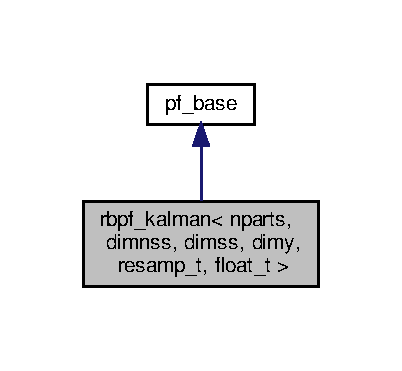
\includegraphics[width=199pt]{classrbpf__kalman__inherit__graph}
\end{center}
\end{figure}


Collaboration diagram for rbpf\+\_\+kalman$<$ nparts, dimnss, dimss, dimy, resamp\+\_\+t, float\+\_\+t $>$\+:\nopagebreak
\begin{figure}[H]
\begin{center}
\leavevmode
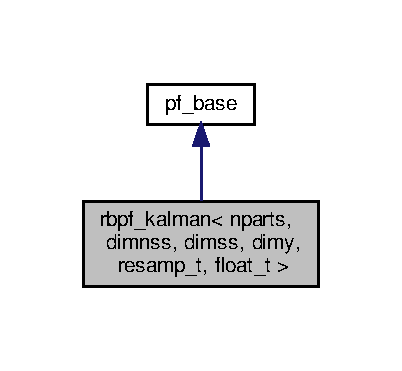
\includegraphics[width=199pt]{classrbpf__kalman__coll__graph}
\end{center}
\end{figure}
\subsection*{Public Types}
\begin{DoxyCompactItemize}
\item 
using \hyperlink{classrbpf__kalman_a616e56c08c1a6b476e065b2200433915}{sssv} = Eigen\+::\+Matrix$<$ float\+\_\+t, dimss, 1 $>$
\item 
using \hyperlink{classrbpf__kalman_aea6e6dd087b2fca63be4e480dcf0d1c3}{nsssv} = Eigen\+::\+Matrix$<$ float\+\_\+t, dimnss, 1 $>$
\item 
using \hyperlink{classrbpf__kalman_ae6e59c034c1b0abc7871887ae088055e}{osv} = Eigen\+::\+Matrix$<$ float\+\_\+t, dimy, 1 $>$
\item 
using \hyperlink{classrbpf__kalman_a736704f31949e04f537aa8b7263e44af}{Mat} = Eigen\+::\+Matrix$<$ float\+\_\+t, Eigen\+::\+Dynamic, Eigen\+::\+Dynamic $>$
\item 
using \hyperlink{classrbpf__kalman_afb337a9e8f4048c0eae2971ea61f96d5}{nsss\+Mat} = Eigen\+::\+Matrix$<$ float\+\_\+t, dimnss, dimnss $>$
\item 
using \hyperlink{classrbpf__kalman_a99e5cb365f01f83962440f29357744d9}{array\+Mod} = std\+::array$<$ \hyperlink{classkalman}{kalman}$<$ dimnss, dimy, 0, float\+\_\+t $>$, nparts $>$
\item 
using \hyperlink{classrbpf__kalman_ad0c2ef4db6363157244741517daae136}{array\+Vec} = std\+::array$<$ \hyperlink{classrbpf__kalman_a616e56c08c1a6b476e065b2200433915}{sssv}, nparts $>$
\item 
using \hyperlink{classrbpf__kalman_a77493b35e7848d5bd91904701adabbbc}{arrayfloat\+\_\+t} = std\+::array$<$ float\+\_\+t, nparts $>$
\end{DoxyCompactItemize}
\subsection*{Public Member Functions}
\begin{DoxyCompactItemize}
\item 
\hyperlink{classrbpf__kalman_a1e128a8dce0874251839b88d1f3cf123}{rbpf\+\_\+kalman} (const unsigned int \&resamp\+\_\+sched=1)
\begin{DoxyCompactList}\small\item\em The constructor. \end{DoxyCompactList}\item 
void \hyperlink{classrbpf__kalman_aad12bf3b1966d7201922770b90429bf0}{filter} (const \hyperlink{classrbpf__kalman_ae6e59c034c1b0abc7871887ae088055e}{osv} \&data, const std\+::vector$<$ std\+::function$<$ const \hyperlink{classrbpf__kalman_a736704f31949e04f537aa8b7263e44af}{Mat}(const \hyperlink{classrbpf__kalman_aea6e6dd087b2fca63be4e480dcf0d1c3}{nsssv} \&x1t, const \hyperlink{classrbpf__kalman_a616e56c08c1a6b476e065b2200433915}{sssv} \&x2t)$>$ $>$ \&fs=std\+::vector$<$ std\+::function$<$ const \hyperlink{classrbpf__kalman_a736704f31949e04f537aa8b7263e44af}{Mat}(const \hyperlink{classrbpf__kalman_aea6e6dd087b2fca63be4e480dcf0d1c3}{nsssv} \&x1t, const \hyperlink{classrbpf__kalman_a616e56c08c1a6b476e065b2200433915}{sssv} \&x2t)$>$ $>$())
\begin{DoxyCompactList}\small\item\em Filter! \end{DoxyCompactList}\item 
float\+\_\+t \hyperlink{classrbpf__kalman_a90d76b85bf97e0f774788e5ccc3aaf8b}{get\+Log\+Cond\+Like} () const
\begin{DoxyCompactList}\small\item\em Get the latest log conditional likelihood. \end{DoxyCompactList}\item 
std\+::vector$<$ \hyperlink{classrbpf__kalman_a736704f31949e04f537aa8b7263e44af}{Mat} $>$ \hyperlink{classrbpf__kalman_a14b715a91d8b8f8bd24946dacc449b18}{get\+Expectations} () const
\begin{DoxyCompactList}\small\item\em Get the latest filtered expectation E\mbox{[}h(x\+\_\+1t, x\+\_\+2t) $\vert$ y\+\_\+\{1\+:t\}\mbox{]}. \end{DoxyCompactList}\item 
virtual float\+\_\+t \hyperlink{classrbpf__kalman_a7040efe459b2346aa8c06a3013f3887c}{log\+Mu\+Ev} (const \hyperlink{classrbpf__kalman_a616e56c08c1a6b476e065b2200433915}{sssv} \&x21)=0
\begin{DoxyCompactList}\small\item\em Evaluates the first time state density. \end{DoxyCompactList}\item 
virtual \hyperlink{classrbpf__kalman_a616e56c08c1a6b476e065b2200433915}{sssv} \hyperlink{classrbpf__kalman_aef30f1f668a823347f7860ac38341233}{q1\+Samp} (const \hyperlink{classrbpf__kalman_ae6e59c034c1b0abc7871887ae088055e}{osv} \&y1)=0
\begin{DoxyCompactList}\small\item\em Sample from the first time\textquotesingle{}s proposal distribution. \end{DoxyCompactList}\item 
virtual \hyperlink{classrbpf__kalman_aea6e6dd087b2fca63be4e480dcf0d1c3}{nsssv} \hyperlink{classrbpf__kalman_a799862d3fb775aed84ce58e00dbce458}{init\+Kalman\+Mean} (const \hyperlink{classrbpf__kalman_a616e56c08c1a6b476e065b2200433915}{sssv} \&x21)=0
\begin{DoxyCompactList}\small\item\em Provides the initial mean vector for each Kalman filter object. \end{DoxyCompactList}\item 
virtual \hyperlink{classrbpf__kalman_afb337a9e8f4048c0eae2971ea61f96d5}{nsss\+Mat} \hyperlink{classrbpf__kalman_ac74007e577ea168e89da9e04cefc8c65}{init\+Kalman\+Var} (const \hyperlink{classrbpf__kalman_a616e56c08c1a6b476e065b2200433915}{sssv} \&x21)=0
\begin{DoxyCompactList}\small\item\em Provides the initial covariance matrix for each Kalman filter object. \end{DoxyCompactList}\item 
virtual \hyperlink{classrbpf__kalman_a616e56c08c1a6b476e065b2200433915}{sssv} \hyperlink{classrbpf__kalman_a03a9dce900a6a917f58f43cbcb906867}{q\+Samp} (const \hyperlink{classrbpf__kalman_a616e56c08c1a6b476e065b2200433915}{sssv} \&x2tm1, const \hyperlink{classrbpf__kalman_ae6e59c034c1b0abc7871887ae088055e}{osv} \&yt)=0
\begin{DoxyCompactList}\small\item\em Samples the time t second component. \end{DoxyCompactList}\item 
virtual float\+\_\+t \hyperlink{classrbpf__kalman_aa9f14f59792b7de573439e318e0a451b}{log\+Q1\+Ev} (const \hyperlink{classrbpf__kalman_a616e56c08c1a6b476e065b2200433915}{sssv} \&x21, const \hyperlink{classrbpf__kalman_ae6e59c034c1b0abc7871887ae088055e}{osv} \&y1)=0
\begin{DoxyCompactList}\small\item\em Evaluates the proposal density of the second state component at time 1. \end{DoxyCompactList}\item 
virtual float\+\_\+t \hyperlink{classrbpf__kalman_ab14d5ef38a664067a2eaec1b3ada1abc}{log\+F\+Ev} (const \hyperlink{classrbpf__kalman_a616e56c08c1a6b476e065b2200433915}{sssv} \&x2t, const \hyperlink{classrbpf__kalman_a616e56c08c1a6b476e065b2200433915}{sssv} \&x2tm1)=0
\begin{DoxyCompactList}\small\item\em Evaluates the state transition density for the second state component. \end{DoxyCompactList}\item 
virtual float\+\_\+t \hyperlink{classrbpf__kalman_a532c85ee43223a4c727de2d636ee8e45}{log\+Q\+Ev} (const \hyperlink{classrbpf__kalman_a616e56c08c1a6b476e065b2200433915}{sssv} \&x2t, const \hyperlink{classrbpf__kalman_a616e56c08c1a6b476e065b2200433915}{sssv} \&x2tm1, const \hyperlink{classrbpf__kalman_ae6e59c034c1b0abc7871887ae088055e}{osv} \&yt)=0
\begin{DoxyCompactList}\small\item\em Evaluates the proposal density at time t $>$ 1. \end{DoxyCompactList}\item 
virtual void \hyperlink{classrbpf__kalman_a1d4dac41b89e8bfd6f54d10c737d4e42}{update\+Kalman} (\hyperlink{classkalman}{kalman}$<$ dimnss, dimy, 0, float\+\_\+t $>$ \&k\+Mod, const \hyperlink{classrbpf__kalman_ae6e59c034c1b0abc7871887ae088055e}{osv} \&yt, const \hyperlink{classrbpf__kalman_a616e56c08c1a6b476e065b2200433915}{sssv} \&x2t)=0
\begin{DoxyCompactList}\small\item\em How to update your inner Kalman filter object at each time. \end{DoxyCompactList}\end{DoxyCompactItemize}
\subsection*{Private Attributes}
\begin{DoxyCompactItemize}
\item 
unsigned int \hyperlink{classrbpf__kalman_a625192fecb630044a08a445f0abb7cdf}{m\+\_\+rs}
\item 
\hyperlink{classrbpf__kalman_a99e5cb365f01f83962440f29357744d9}{array\+Mod} \hyperlink{classrbpf__kalman_ad6ff53f5ea23c35d3c7154b31a50bb34}{m\+\_\+p\+\_\+inner\+Mods}
\item 
\hyperlink{classrbpf__kalman_ad0c2ef4db6363157244741517daae136}{array\+Vec} \hyperlink{classrbpf__kalman_a88f7188c59b2cc1407a14e60051a1840}{m\+\_\+p\+\_\+samps}
\item 
\hyperlink{classrbpf__kalman_a77493b35e7848d5bd91904701adabbbc}{arrayfloat\+\_\+t} \hyperlink{classrbpf__kalman_a086f86066051a4f955b7b8b922a932af}{m\+\_\+log\+Un\+Norm\+Weights}
\item 
unsigned int \hyperlink{classrbpf__kalman_a0c27a82501d16ed1a8b427c053d47c93}{m\+\_\+now}
\item 
float\+\_\+t \hyperlink{classrbpf__kalman_adb1cf2ea7161d4a6e5a9a7240b9cdff1}{m\+\_\+last\+Log\+Cond\+Like}
\item 
resamp\+\_\+t \hyperlink{classrbpf__kalman_a8ecaad1e77a122988843b2a0a33f882d}{m\+\_\+resampler}
\item 
std\+::vector$<$ \hyperlink{classrbpf__kalman_a736704f31949e04f537aa8b7263e44af}{Mat} $>$ \hyperlink{classrbpf__kalman_ab44eceb581029abcce88710ef7f9c38f}{m\+\_\+expectations}
\end{DoxyCompactItemize}
\subsection*{Additional Inherited Members}


\subsection{Detailed Description}
\subsubsection*{template$<$size\+\_\+t nparts, size\+\_\+t dimnss, size\+\_\+t dimss, size\+\_\+t dimy, typename resamp\+\_\+t, typename float\+\_\+t$>$\newline
class rbpf\+\_\+kalman$<$ nparts, dimnss, dimss, dimy, resamp\+\_\+t, float\+\_\+t $>$}

Rao-\/\+Blackwellized/\+Marginal Particle Filter with inner Kalman Filter objectss. 

\begin{DoxyAuthor}{Author}
t 
\end{DoxyAuthor}


\subsection{Member Typedef Documentation}
\mbox{\Hypertarget{classrbpf__kalman_a77493b35e7848d5bd91904701adabbbc}\label{classrbpf__kalman_a77493b35e7848d5bd91904701adabbbc}} 
\index{rbpf\+\_\+kalman@{rbpf\+\_\+kalman}!arrayfloat\+\_\+t@{arrayfloat\+\_\+t}}
\index{arrayfloat\+\_\+t@{arrayfloat\+\_\+t}!rbpf\+\_\+kalman@{rbpf\+\_\+kalman}}
\subsubsection{\texorpdfstring{arrayfloat\+\_\+t}{arrayfloat\_t}}
{\footnotesize\ttfamily template$<$size\+\_\+t nparts, size\+\_\+t dimnss, size\+\_\+t dimss, size\+\_\+t dimy, typename resamp\+\_\+t , typename float\+\_\+t $>$ \\
using \hyperlink{classrbpf__kalman}{rbpf\+\_\+kalman}$<$ nparts, dimnss, dimss, dimy, resamp\+\_\+t, float\+\_\+t $>$\+::\hyperlink{classrbpf__kalman_a77493b35e7848d5bd91904701adabbbc}{arrayfloat\+\_\+t} =  std\+::array$<$float\+\_\+t,nparts$>$}

array of weights \mbox{\Hypertarget{classrbpf__kalman_a99e5cb365f01f83962440f29357744d9}\label{classrbpf__kalman_a99e5cb365f01f83962440f29357744d9}} 
\index{rbpf\+\_\+kalman@{rbpf\+\_\+kalman}!array\+Mod@{array\+Mod}}
\index{array\+Mod@{array\+Mod}!rbpf\+\_\+kalman@{rbpf\+\_\+kalman}}
\subsubsection{\texorpdfstring{array\+Mod}{arrayMod}}
{\footnotesize\ttfamily template$<$size\+\_\+t nparts, size\+\_\+t dimnss, size\+\_\+t dimss, size\+\_\+t dimy, typename resamp\+\_\+t , typename float\+\_\+t $>$ \\
using \hyperlink{classrbpf__kalman}{rbpf\+\_\+kalman}$<$ nparts, dimnss, dimss, dimy, resamp\+\_\+t, float\+\_\+t $>$\+::\hyperlink{classrbpf__kalman_a99e5cb365f01f83962440f29357744d9}{array\+Mod} =  std\+::array$<$\hyperlink{classkalman}{kalman}$<$dimnss,dimy,0,float\+\_\+t$>$,nparts$>$}

array of model objects \mbox{\Hypertarget{classrbpf__kalman_ad0c2ef4db6363157244741517daae136}\label{classrbpf__kalman_ad0c2ef4db6363157244741517daae136}} 
\index{rbpf\+\_\+kalman@{rbpf\+\_\+kalman}!array\+Vec@{array\+Vec}}
\index{array\+Vec@{array\+Vec}!rbpf\+\_\+kalman@{rbpf\+\_\+kalman}}
\subsubsection{\texorpdfstring{array\+Vec}{arrayVec}}
{\footnotesize\ttfamily template$<$size\+\_\+t nparts, size\+\_\+t dimnss, size\+\_\+t dimss, size\+\_\+t dimy, typename resamp\+\_\+t , typename float\+\_\+t $>$ \\
using \hyperlink{classrbpf__kalman}{rbpf\+\_\+kalman}$<$ nparts, dimnss, dimss, dimy, resamp\+\_\+t, float\+\_\+t $>$\+::\hyperlink{classrbpf__kalman_ad0c2ef4db6363157244741517daae136}{array\+Vec} =  std\+::array$<$\hyperlink{classrbpf__kalman_a616e56c08c1a6b476e065b2200433915}{sssv},nparts$>$}

array of samples \mbox{\Hypertarget{classrbpf__kalman_a736704f31949e04f537aa8b7263e44af}\label{classrbpf__kalman_a736704f31949e04f537aa8b7263e44af}} 
\index{rbpf\+\_\+kalman@{rbpf\+\_\+kalman}!Mat@{Mat}}
\index{Mat@{Mat}!rbpf\+\_\+kalman@{rbpf\+\_\+kalman}}
\subsubsection{\texorpdfstring{Mat}{Mat}}
{\footnotesize\ttfamily template$<$size\+\_\+t nparts, size\+\_\+t dimnss, size\+\_\+t dimss, size\+\_\+t dimy, typename resamp\+\_\+t , typename float\+\_\+t $>$ \\
using \hyperlink{classrbpf__kalman}{rbpf\+\_\+kalman}$<$ nparts, dimnss, dimss, dimy, resamp\+\_\+t, float\+\_\+t $>$\+::\hyperlink{classrbpf__kalman_a736704f31949e04f537aa8b7263e44af}{Mat} =  Eigen\+::\+Matrix$<$float\+\_\+t,Eigen\+::\+Dynamic,Eigen\+::\+Dynamic$>$}

dynamic size matrices \mbox{\Hypertarget{classrbpf__kalman_afb337a9e8f4048c0eae2971ea61f96d5}\label{classrbpf__kalman_afb337a9e8f4048c0eae2971ea61f96d5}} 
\index{rbpf\+\_\+kalman@{rbpf\+\_\+kalman}!nsss\+Mat@{nsss\+Mat}}
\index{nsss\+Mat@{nsss\+Mat}!rbpf\+\_\+kalman@{rbpf\+\_\+kalman}}
\subsubsection{\texorpdfstring{nsss\+Mat}{nsssMat}}
{\footnotesize\ttfamily template$<$size\+\_\+t nparts, size\+\_\+t dimnss, size\+\_\+t dimss, size\+\_\+t dimy, typename resamp\+\_\+t , typename float\+\_\+t $>$ \\
using \hyperlink{classrbpf__kalman}{rbpf\+\_\+kalman}$<$ nparts, dimnss, dimss, dimy, resamp\+\_\+t, float\+\_\+t $>$\+::\hyperlink{classrbpf__kalman_afb337a9e8f4048c0eae2971ea61f96d5}{nsss\+Mat} =  Eigen\+::\+Matrix$<$float\+\_\+t,dimnss,dimnss$>$}

\char`\"{}not sampled state size matrix\char`\"{} \mbox{\Hypertarget{classrbpf__kalman_aea6e6dd087b2fca63be4e480dcf0d1c3}\label{classrbpf__kalman_aea6e6dd087b2fca63be4e480dcf0d1c3}} 
\index{rbpf\+\_\+kalman@{rbpf\+\_\+kalman}!nsssv@{nsssv}}
\index{nsssv@{nsssv}!rbpf\+\_\+kalman@{rbpf\+\_\+kalman}}
\subsubsection{\texorpdfstring{nsssv}{nsssv}}
{\footnotesize\ttfamily template$<$size\+\_\+t nparts, size\+\_\+t dimnss, size\+\_\+t dimss, size\+\_\+t dimy, typename resamp\+\_\+t , typename float\+\_\+t $>$ \\
using \hyperlink{classrbpf__kalman}{rbpf\+\_\+kalman}$<$ nparts, dimnss, dimss, dimy, resamp\+\_\+t, float\+\_\+t $>$\+::\hyperlink{classrbpf__kalman_aea6e6dd087b2fca63be4e480dcf0d1c3}{nsssv} =  Eigen\+::\+Matrix$<$float\+\_\+t,dimnss,1$>$}

\char`\"{}not sampled state size vector\char`\"{} \mbox{\Hypertarget{classrbpf__kalman_ae6e59c034c1b0abc7871887ae088055e}\label{classrbpf__kalman_ae6e59c034c1b0abc7871887ae088055e}} 
\index{rbpf\+\_\+kalman@{rbpf\+\_\+kalman}!osv@{osv}}
\index{osv@{osv}!rbpf\+\_\+kalman@{rbpf\+\_\+kalman}}
\subsubsection{\texorpdfstring{osv}{osv}}
{\footnotesize\ttfamily template$<$size\+\_\+t nparts, size\+\_\+t dimnss, size\+\_\+t dimss, size\+\_\+t dimy, typename resamp\+\_\+t , typename float\+\_\+t $>$ \\
using \hyperlink{classrbpf__kalman}{rbpf\+\_\+kalman}$<$ nparts, dimnss, dimss, dimy, resamp\+\_\+t, float\+\_\+t $>$\+::\hyperlink{classrbpf__kalman_ae6e59c034c1b0abc7871887ae088055e}{osv} =  Eigen\+::\+Matrix$<$float\+\_\+t,dimy,1$>$}

\char`\"{}observation size vector\char`\"{} \mbox{\Hypertarget{classrbpf__kalman_a616e56c08c1a6b476e065b2200433915}\label{classrbpf__kalman_a616e56c08c1a6b476e065b2200433915}} 
\index{rbpf\+\_\+kalman@{rbpf\+\_\+kalman}!sssv@{sssv}}
\index{sssv@{sssv}!rbpf\+\_\+kalman@{rbpf\+\_\+kalman}}
\subsubsection{\texorpdfstring{sssv}{sssv}}
{\footnotesize\ttfamily template$<$size\+\_\+t nparts, size\+\_\+t dimnss, size\+\_\+t dimss, size\+\_\+t dimy, typename resamp\+\_\+t , typename float\+\_\+t $>$ \\
using \hyperlink{classrbpf__kalman}{rbpf\+\_\+kalman}$<$ nparts, dimnss, dimss, dimy, resamp\+\_\+t, float\+\_\+t $>$\+::\hyperlink{classrbpf__kalman_a616e56c08c1a6b476e065b2200433915}{sssv} =  Eigen\+::\+Matrix$<$float\+\_\+t,dimss,1$>$}

\char`\"{}sampled state size vector\char`\"{} 

\subsection{Constructor \& Destructor Documentation}
\mbox{\Hypertarget{classrbpf__kalman_a1e128a8dce0874251839b88d1f3cf123}\label{classrbpf__kalman_a1e128a8dce0874251839b88d1f3cf123}} 
\index{rbpf\+\_\+kalman@{rbpf\+\_\+kalman}!rbpf\+\_\+kalman@{rbpf\+\_\+kalman}}
\index{rbpf\+\_\+kalman@{rbpf\+\_\+kalman}!rbpf\+\_\+kalman@{rbpf\+\_\+kalman}}
\subsubsection{\texorpdfstring{rbpf\+\_\+kalman()}{rbpf\_kalman()}}
{\footnotesize\ttfamily template$<$size\+\_\+t nparts, size\+\_\+t dimnss, size\+\_\+t dimss, size\+\_\+t dimy, typename resamp\+\_\+t , typename float\+\_\+t $>$ \\
\hyperlink{classrbpf__kalman}{rbpf\+\_\+kalman}$<$ nparts, dimnss, dimss, dimy, resamp\+\_\+t, float\+\_\+t $>$\+::\hyperlink{classrbpf__kalman}{rbpf\+\_\+kalman} (\begin{DoxyParamCaption}\item[{const unsigned int \&}]{resamp\+\_\+sched = {\ttfamily 1} }\end{DoxyParamCaption})}



The constructor. 


\begin{DoxyParams}{Parameters}
{\em resamp\+\_\+sched} & how often you want to resample (e.\+g once every resamp\+\_\+sched time points) \\
\hline
\end{DoxyParams}


\subsection{Member Function Documentation}
\mbox{\Hypertarget{classrbpf__kalman_aad12bf3b1966d7201922770b90429bf0}\label{classrbpf__kalman_aad12bf3b1966d7201922770b90429bf0}} 
\index{rbpf\+\_\+kalman@{rbpf\+\_\+kalman}!filter@{filter}}
\index{filter@{filter}!rbpf\+\_\+kalman@{rbpf\+\_\+kalman}}
\subsubsection{\texorpdfstring{filter()}{filter()}}
{\footnotesize\ttfamily template$<$size\+\_\+t nparts, size\+\_\+t dimnss, size\+\_\+t dimss, size\+\_\+t dimy, typename resamp\+\_\+t , typename float\+\_\+t $>$ \\
void \hyperlink{classrbpf__kalman}{rbpf\+\_\+kalman}$<$ nparts, dimnss, dimss, dimy, resamp\+\_\+t, float\+\_\+t $>$\+::filter (\begin{DoxyParamCaption}\item[{const \hyperlink{classrbpf__kalman_ae6e59c034c1b0abc7871887ae088055e}{osv} \&}]{data,  }\item[{const std\+::vector$<$ std\+::function$<$ const \hyperlink{classrbpf__kalman_a736704f31949e04f537aa8b7263e44af}{Mat}(const \hyperlink{classrbpf__kalman_aea6e6dd087b2fca63be4e480dcf0d1c3}{nsssv} \&x1t, const \hyperlink{classrbpf__kalman_a616e56c08c1a6b476e065b2200433915}{sssv} \&x2t)$>$ $>$ \&}]{fs = {\ttfamily std\+:\+:vector$<$std\+:\+:function$<$const~\hyperlink{classrbpf__kalman_a736704f31949e04f537aa8b7263e44af}{Mat}(const~\hyperlink{classrbpf__kalman_aea6e6dd087b2fca63be4e480dcf0d1c3}{nsssv}~\&x1t,~const~\hyperlink{classrbpf__kalman_a616e56c08c1a6b476e065b2200433915}{sssv}~\&x2t)$>$~$>$()} }\end{DoxyParamCaption})}



Filter! 

The workhorse function 
\begin{DoxyParams}{Parameters}
{\em data} & the most recent observable portion of the time series. \\
\hline
{\em fs} & a vector of functions computing E\mbox{[}h(x\+\_\+1t, x\+\_\+2t$^\wedge$i)$\vert$ x\+\_\+2t$^\wedge$i,y\+\_\+1\+:t\mbox{]}. to be averaged to yield E\mbox{[}h(x\+\_\+1t, x\+\_\+2t)$\vert$,y\+\_\+1\+:t\mbox{]} \\
\hline
\end{DoxyParams}
\mbox{\Hypertarget{classrbpf__kalman_a14b715a91d8b8f8bd24946dacc449b18}\label{classrbpf__kalman_a14b715a91d8b8f8bd24946dacc449b18}} 
\index{rbpf\+\_\+kalman@{rbpf\+\_\+kalman}!get\+Expectations@{get\+Expectations}}
\index{get\+Expectations@{get\+Expectations}!rbpf\+\_\+kalman@{rbpf\+\_\+kalman}}
\subsubsection{\texorpdfstring{get\+Expectations()}{getExpectations()}}
{\footnotesize\ttfamily template$<$size\+\_\+t nparts, size\+\_\+t dimnss, size\+\_\+t dimss, size\+\_\+t dimy, typename resamp\+\_\+t , typename float\+\_\+t $>$ \\
auto \hyperlink{classrbpf__kalman}{rbpf\+\_\+kalman}$<$ nparts, dimnss, dimss, dimy, resamp\+\_\+t, float\+\_\+t $>$\+::get\+Expectations (\begin{DoxyParamCaption}{ }\end{DoxyParamCaption}) const}



Get the latest filtered expectation E\mbox{[}h(x\+\_\+1t, x\+\_\+2t) $\vert$ y\+\_\+\{1\+:t\}\mbox{]}. 

Get the expectations you\textquotesingle{}re keeping track of. \begin{DoxyReturn}{Returns}
a vector of Mats 
\end{DoxyReturn}
\mbox{\Hypertarget{classrbpf__kalman_a90d76b85bf97e0f774788e5ccc3aaf8b}\label{classrbpf__kalman_a90d76b85bf97e0f774788e5ccc3aaf8b}} 
\index{rbpf\+\_\+kalman@{rbpf\+\_\+kalman}!get\+Log\+Cond\+Like@{get\+Log\+Cond\+Like}}
\index{get\+Log\+Cond\+Like@{get\+Log\+Cond\+Like}!rbpf\+\_\+kalman@{rbpf\+\_\+kalman}}
\subsubsection{\texorpdfstring{get\+Log\+Cond\+Like()}{getLogCondLike()}}
{\footnotesize\ttfamily template$<$size\+\_\+t nparts, size\+\_\+t dimnss, size\+\_\+t dimss, size\+\_\+t dimy, typename resamp\+\_\+t , typename float\+\_\+t $>$ \\
float\+\_\+t \hyperlink{classrbpf__kalman}{rbpf\+\_\+kalman}$<$ nparts, dimnss, dimss, dimy, resamp\+\_\+t, float\+\_\+t $>$\+::get\+Log\+Cond\+Like (\begin{DoxyParamCaption}{ }\end{DoxyParamCaption}) const}



Get the latest log conditional likelihood. 

\begin{DoxyReturn}{Returns}
the latest log conditional likelihood. 
\end{DoxyReturn}
\mbox{\Hypertarget{classrbpf__kalman_a799862d3fb775aed84ce58e00dbce458}\label{classrbpf__kalman_a799862d3fb775aed84ce58e00dbce458}} 
\index{rbpf\+\_\+kalman@{rbpf\+\_\+kalman}!init\+Kalman\+Mean@{init\+Kalman\+Mean}}
\index{init\+Kalman\+Mean@{init\+Kalman\+Mean}!rbpf\+\_\+kalman@{rbpf\+\_\+kalman}}
\subsubsection{\texorpdfstring{init\+Kalman\+Mean()}{initKalmanMean()}}
{\footnotesize\ttfamily template$<$size\+\_\+t nparts, size\+\_\+t dimnss, size\+\_\+t dimss, size\+\_\+t dimy, typename resamp\+\_\+t , typename float\+\_\+t $>$ \\
virtual \hyperlink{classrbpf__kalman_aea6e6dd087b2fca63be4e480dcf0d1c3}{nsssv} \hyperlink{classrbpf__kalman}{rbpf\+\_\+kalman}$<$ nparts, dimnss, dimss, dimy, resamp\+\_\+t, float\+\_\+t $>$\+::init\+Kalman\+Mean (\begin{DoxyParamCaption}\item[{const \hyperlink{classrbpf__kalman_a616e56c08c1a6b476e065b2200433915}{sssv} \&}]{x21 }\end{DoxyParamCaption})\hspace{0.3cm}{\ttfamily [pure virtual]}}



Provides the initial mean vector for each Kalman filter object. 

provides the initial mean vector for each Kalman filter object. 
\begin{DoxyParams}{Parameters}
{\em x21} & the second state componenent at time 1. \\
\hline
\end{DoxyParams}
\begin{DoxyReturn}{Returns}
a nsssv representing the unconditional mean. 
\end{DoxyReturn}
\mbox{\Hypertarget{classrbpf__kalman_ac74007e577ea168e89da9e04cefc8c65}\label{classrbpf__kalman_ac74007e577ea168e89da9e04cefc8c65}} 
\index{rbpf\+\_\+kalman@{rbpf\+\_\+kalman}!init\+Kalman\+Var@{init\+Kalman\+Var}}
\index{init\+Kalman\+Var@{init\+Kalman\+Var}!rbpf\+\_\+kalman@{rbpf\+\_\+kalman}}
\subsubsection{\texorpdfstring{init\+Kalman\+Var()}{initKalmanVar()}}
{\footnotesize\ttfamily template$<$size\+\_\+t nparts, size\+\_\+t dimnss, size\+\_\+t dimss, size\+\_\+t dimy, typename resamp\+\_\+t , typename float\+\_\+t $>$ \\
virtual \hyperlink{classrbpf__kalman_afb337a9e8f4048c0eae2971ea61f96d5}{nsss\+Mat} \hyperlink{classrbpf__kalman}{rbpf\+\_\+kalman}$<$ nparts, dimnss, dimss, dimy, resamp\+\_\+t, float\+\_\+t $>$\+::init\+Kalman\+Var (\begin{DoxyParamCaption}\item[{const \hyperlink{classrbpf__kalman_a616e56c08c1a6b476e065b2200433915}{sssv} \&}]{x21 }\end{DoxyParamCaption})\hspace{0.3cm}{\ttfamily [pure virtual]}}



Provides the initial covariance matrix for each Kalman filter object. 

provides the initial covariance matrix for each Kalman filter object. 
\begin{DoxyParams}{Parameters}
{\em x21} & the second state component at time 1. \\
\hline
\end{DoxyParams}
\begin{DoxyReturn}{Returns}
a covariance matrix. 
\end{DoxyReturn}
\mbox{\Hypertarget{classrbpf__kalman_ab14d5ef38a664067a2eaec1b3ada1abc}\label{classrbpf__kalman_ab14d5ef38a664067a2eaec1b3ada1abc}} 
\index{rbpf\+\_\+kalman@{rbpf\+\_\+kalman}!log\+F\+Ev@{log\+F\+Ev}}
\index{log\+F\+Ev@{log\+F\+Ev}!rbpf\+\_\+kalman@{rbpf\+\_\+kalman}}
\subsubsection{\texorpdfstring{log\+F\+Ev()}{logFEv()}}
{\footnotesize\ttfamily template$<$size\+\_\+t nparts, size\+\_\+t dimnss, size\+\_\+t dimss, size\+\_\+t dimy, typename resamp\+\_\+t , typename float\+\_\+t $>$ \\
virtual float\+\_\+t \hyperlink{classrbpf__kalman}{rbpf\+\_\+kalman}$<$ nparts, dimnss, dimss, dimy, resamp\+\_\+t, float\+\_\+t $>$\+::log\+F\+Ev (\begin{DoxyParamCaption}\item[{const \hyperlink{classrbpf__kalman_a616e56c08c1a6b476e065b2200433915}{sssv} \&}]{x2t,  }\item[{const \hyperlink{classrbpf__kalman_a616e56c08c1a6b476e065b2200433915}{sssv} \&}]{x2tm1 }\end{DoxyParamCaption})\hspace{0.3cm}{\ttfamily [pure virtual]}}



Evaluates the state transition density for the second state component. 

Evaluates the state transition density for the second state component. 
\begin{DoxyParams}{Parameters}
{\em x2t} & the current second state component. \\
\hline
{\em x2tm1} & the previous second state component. \\
\hline
\end{DoxyParams}
\begin{DoxyReturn}{Returns}
a float\+\_\+t evaluation. 
\end{DoxyReturn}
\mbox{\Hypertarget{classrbpf__kalman_a7040efe459b2346aa8c06a3013f3887c}\label{classrbpf__kalman_a7040efe459b2346aa8c06a3013f3887c}} 
\index{rbpf\+\_\+kalman@{rbpf\+\_\+kalman}!log\+Mu\+Ev@{log\+Mu\+Ev}}
\index{log\+Mu\+Ev@{log\+Mu\+Ev}!rbpf\+\_\+kalman@{rbpf\+\_\+kalman}}
\subsubsection{\texorpdfstring{log\+Mu\+Ev()}{logMuEv()}}
{\footnotesize\ttfamily template$<$size\+\_\+t nparts, size\+\_\+t dimnss, size\+\_\+t dimss, size\+\_\+t dimy, typename resamp\+\_\+t , typename float\+\_\+t $>$ \\
virtual float\+\_\+t \hyperlink{classrbpf__kalman}{rbpf\+\_\+kalman}$<$ nparts, dimnss, dimss, dimy, resamp\+\_\+t, float\+\_\+t $>$\+::log\+Mu\+Ev (\begin{DoxyParamCaption}\item[{const \hyperlink{classrbpf__kalman_a616e56c08c1a6b476e065b2200433915}{sssv} \&}]{x21 }\end{DoxyParamCaption})\hspace{0.3cm}{\ttfamily [pure virtual]}}



Evaluates the first time state density. 

evaluates log mu(x21). 
\begin{DoxyParams}{Parameters}
{\em x21} & component two at time 1 \\
\hline
\end{DoxyParams}
\begin{DoxyReturn}{Returns}
a float\+\_\+t evaluation 
\end{DoxyReturn}
\mbox{\Hypertarget{classrbpf__kalman_aa9f14f59792b7de573439e318e0a451b}\label{classrbpf__kalman_aa9f14f59792b7de573439e318e0a451b}} 
\index{rbpf\+\_\+kalman@{rbpf\+\_\+kalman}!log\+Q1\+Ev@{log\+Q1\+Ev}}
\index{log\+Q1\+Ev@{log\+Q1\+Ev}!rbpf\+\_\+kalman@{rbpf\+\_\+kalman}}
\subsubsection{\texorpdfstring{log\+Q1\+Ev()}{logQ1Ev()}}
{\footnotesize\ttfamily template$<$size\+\_\+t nparts, size\+\_\+t dimnss, size\+\_\+t dimss, size\+\_\+t dimy, typename resamp\+\_\+t , typename float\+\_\+t $>$ \\
virtual float\+\_\+t \hyperlink{classrbpf__kalman}{rbpf\+\_\+kalman}$<$ nparts, dimnss, dimss, dimy, resamp\+\_\+t, float\+\_\+t $>$\+::log\+Q1\+Ev (\begin{DoxyParamCaption}\item[{const \hyperlink{classrbpf__kalman_a616e56c08c1a6b476e065b2200433915}{sssv} \&}]{x21,  }\item[{const \hyperlink{classrbpf__kalman_ae6e59c034c1b0abc7871887ae088055e}{osv} \&}]{y1 }\end{DoxyParamCaption})\hspace{0.3cm}{\ttfamily [pure virtual]}}



Evaluates the proposal density of the second state component at time 1. 

Evaluates the proposal density of the second state component at time 1. 
\begin{DoxyParams}{Parameters}
{\em x21} & the second state component at time 1 you sampled. \\
\hline
{\em y1} & time 1 observation. \\
\hline
\end{DoxyParams}
\begin{DoxyReturn}{Returns}
a float\+\_\+t evaluation of the density. 
\end{DoxyReturn}
\mbox{\Hypertarget{classrbpf__kalman_a532c85ee43223a4c727de2d636ee8e45}\label{classrbpf__kalman_a532c85ee43223a4c727de2d636ee8e45}} 
\index{rbpf\+\_\+kalman@{rbpf\+\_\+kalman}!log\+Q\+Ev@{log\+Q\+Ev}}
\index{log\+Q\+Ev@{log\+Q\+Ev}!rbpf\+\_\+kalman@{rbpf\+\_\+kalman}}
\subsubsection{\texorpdfstring{log\+Q\+Ev()}{logQEv()}}
{\footnotesize\ttfamily template$<$size\+\_\+t nparts, size\+\_\+t dimnss, size\+\_\+t dimss, size\+\_\+t dimy, typename resamp\+\_\+t , typename float\+\_\+t $>$ \\
virtual float\+\_\+t \hyperlink{classrbpf__kalman}{rbpf\+\_\+kalman}$<$ nparts, dimnss, dimss, dimy, resamp\+\_\+t, float\+\_\+t $>$\+::log\+Q\+Ev (\begin{DoxyParamCaption}\item[{const \hyperlink{classrbpf__kalman_a616e56c08c1a6b476e065b2200433915}{sssv} \&}]{x2t,  }\item[{const \hyperlink{classrbpf__kalman_a616e56c08c1a6b476e065b2200433915}{sssv} \&}]{x2tm1,  }\item[{const \hyperlink{classrbpf__kalman_ae6e59c034c1b0abc7871887ae088055e}{osv} \&}]{yt }\end{DoxyParamCaption})\hspace{0.3cm}{\ttfamily [pure virtual]}}



Evaluates the proposal density at time t $>$ 1. 

Evaluates the proposal density at time t $>$ 1. 
\begin{DoxyParams}{Parameters}
{\em x2t} & the current second state component. \\
\hline
{\em x2tm1} & the previous second state component. \\
\hline
{\em yt} & the current time series observation. \\
\hline
\end{DoxyParams}
\begin{DoxyReturn}{Returns}
a float\+\_\+t evaluation. 
\end{DoxyReturn}
\mbox{\Hypertarget{classrbpf__kalman_aef30f1f668a823347f7860ac38341233}\label{classrbpf__kalman_aef30f1f668a823347f7860ac38341233}} 
\index{rbpf\+\_\+kalman@{rbpf\+\_\+kalman}!q1\+Samp@{q1\+Samp}}
\index{q1\+Samp@{q1\+Samp}!rbpf\+\_\+kalman@{rbpf\+\_\+kalman}}
\subsubsection{\texorpdfstring{q1\+Samp()}{q1Samp()}}
{\footnotesize\ttfamily template$<$size\+\_\+t nparts, size\+\_\+t dimnss, size\+\_\+t dimss, size\+\_\+t dimy, typename resamp\+\_\+t , typename float\+\_\+t $>$ \\
virtual \hyperlink{classrbpf__kalman_a616e56c08c1a6b476e065b2200433915}{sssv} \hyperlink{classrbpf__kalman}{rbpf\+\_\+kalman}$<$ nparts, dimnss, dimss, dimy, resamp\+\_\+t, float\+\_\+t $>$\+::q1\+Samp (\begin{DoxyParamCaption}\item[{const \hyperlink{classrbpf__kalman_ae6e59c034c1b0abc7871887ae088055e}{osv} \&}]{y1 }\end{DoxyParamCaption})\hspace{0.3cm}{\ttfamily [pure virtual]}}



Sample from the first time\textquotesingle{}s proposal distribution. 

samples the second component of the state at time 1. 
\begin{DoxyParams}{Parameters}
{\em y1} & most recent datum. \\
\hline
\end{DoxyParams}
\begin{DoxyReturn}{Returns}
a Vec sample for x21. 
\end{DoxyReturn}
\mbox{\Hypertarget{classrbpf__kalman_a03a9dce900a6a917f58f43cbcb906867}\label{classrbpf__kalman_a03a9dce900a6a917f58f43cbcb906867}} 
\index{rbpf\+\_\+kalman@{rbpf\+\_\+kalman}!q\+Samp@{q\+Samp}}
\index{q\+Samp@{q\+Samp}!rbpf\+\_\+kalman@{rbpf\+\_\+kalman}}
\subsubsection{\texorpdfstring{q\+Samp()}{qSamp()}}
{\footnotesize\ttfamily template$<$size\+\_\+t nparts, size\+\_\+t dimnss, size\+\_\+t dimss, size\+\_\+t dimy, typename resamp\+\_\+t , typename float\+\_\+t $>$ \\
virtual \hyperlink{classrbpf__kalman_a616e56c08c1a6b476e065b2200433915}{sssv} \hyperlink{classrbpf__kalman}{rbpf\+\_\+kalman}$<$ nparts, dimnss, dimss, dimy, resamp\+\_\+t, float\+\_\+t $>$\+::q\+Samp (\begin{DoxyParamCaption}\item[{const \hyperlink{classrbpf__kalman_a616e56c08c1a6b476e065b2200433915}{sssv} \&}]{x2tm1,  }\item[{const \hyperlink{classrbpf__kalman_ae6e59c034c1b0abc7871887ae088055e}{osv} \&}]{yt }\end{DoxyParamCaption})\hspace{0.3cm}{\ttfamily [pure virtual]}}



Samples the time t second component. 

Samples the time t second component. 
\begin{DoxyParams}{Parameters}
{\em x2tm1} & the previous time\textquotesingle{}s second state component. \\
\hline
{\em yt} & the current observation. \\
\hline
\end{DoxyParams}
\begin{DoxyReturn}{Returns}
a sssv sample of the second state component at the current time. 
\end{DoxyReturn}
\mbox{\Hypertarget{classrbpf__kalman_a1d4dac41b89e8bfd6f54d10c737d4e42}\label{classrbpf__kalman_a1d4dac41b89e8bfd6f54d10c737d4e42}} 
\index{rbpf\+\_\+kalman@{rbpf\+\_\+kalman}!update\+Kalman@{update\+Kalman}}
\index{update\+Kalman@{update\+Kalman}!rbpf\+\_\+kalman@{rbpf\+\_\+kalman}}
\subsubsection{\texorpdfstring{update\+Kalman()}{updateKalman()}}
{\footnotesize\ttfamily template$<$size\+\_\+t nparts, size\+\_\+t dimnss, size\+\_\+t dimss, size\+\_\+t dimy, typename resamp\+\_\+t , typename float\+\_\+t $>$ \\
virtual void \hyperlink{classrbpf__kalman}{rbpf\+\_\+kalman}$<$ nparts, dimnss, dimss, dimy, resamp\+\_\+t, float\+\_\+t $>$\+::update\+Kalman (\begin{DoxyParamCaption}\item[{\hyperlink{classkalman}{kalman}$<$ dimnss, dimy, 0, float\+\_\+t $>$ \&}]{k\+Mod,  }\item[{const \hyperlink{classrbpf__kalman_ae6e59c034c1b0abc7871887ae088055e}{osv} \&}]{yt,  }\item[{const \hyperlink{classrbpf__kalman_a616e56c08c1a6b476e065b2200433915}{sssv} \&}]{x2t }\end{DoxyParamCaption})\hspace{0.3cm}{\ttfamily [pure virtual]}}



How to update your inner Kalman filter object at each time. 

How to update your inner Kalman filter object at each time. 
\begin{DoxyParams}{Parameters}
{\em k\+Mod} & a Kalman filter object describing the conditional closed-\/form model. \\
\hline
{\em yt} & the current time series observation. \\
\hline
{\em x2t} & the current second state component. \\
\hline
\end{DoxyParams}


\subsection{Member Data Documentation}
\mbox{\Hypertarget{classrbpf__kalman_ab44eceb581029abcce88710ef7f9c38f}\label{classrbpf__kalman_ab44eceb581029abcce88710ef7f9c38f}} 
\index{rbpf\+\_\+kalman@{rbpf\+\_\+kalman}!m\+\_\+expectations@{m\+\_\+expectations}}
\index{m\+\_\+expectations@{m\+\_\+expectations}!rbpf\+\_\+kalman@{rbpf\+\_\+kalman}}
\subsubsection{\texorpdfstring{m\+\_\+expectations}{m\_expectations}}
{\footnotesize\ttfamily template$<$size\+\_\+t nparts, size\+\_\+t dimnss, size\+\_\+t dimss, size\+\_\+t dimy, typename resamp\+\_\+t , typename float\+\_\+t $>$ \\
std\+::vector$<$\hyperlink{classrbpf__kalman_a736704f31949e04f537aa8b7263e44af}{Mat}$>$ \hyperlink{classrbpf__kalman}{rbpf\+\_\+kalman}$<$ nparts, dimnss, dimss, dimy, resamp\+\_\+t, float\+\_\+t $>$\+::m\+\_\+expectations\hspace{0.3cm}{\ttfamily [private]}}

expectations \mbox{\Hypertarget{classrbpf__kalman_adb1cf2ea7161d4a6e5a9a7240b9cdff1}\label{classrbpf__kalman_adb1cf2ea7161d4a6e5a9a7240b9cdff1}} 
\index{rbpf\+\_\+kalman@{rbpf\+\_\+kalman}!m\+\_\+last\+Log\+Cond\+Like@{m\+\_\+last\+Log\+Cond\+Like}}
\index{m\+\_\+last\+Log\+Cond\+Like@{m\+\_\+last\+Log\+Cond\+Like}!rbpf\+\_\+kalman@{rbpf\+\_\+kalman}}
\subsubsection{\texorpdfstring{m\+\_\+last\+Log\+Cond\+Like}{m\_lastLogCondLike}}
{\footnotesize\ttfamily template$<$size\+\_\+t nparts, size\+\_\+t dimnss, size\+\_\+t dimss, size\+\_\+t dimy, typename resamp\+\_\+t , typename float\+\_\+t $>$ \\
float\+\_\+t \hyperlink{classrbpf__kalman}{rbpf\+\_\+kalman}$<$ nparts, dimnss, dimss, dimy, resamp\+\_\+t, float\+\_\+t $>$\+::m\+\_\+last\+Log\+Cond\+Like\hspace{0.3cm}{\ttfamily [private]}}

log p(y\+\_\+t$\vert$y\+\_\+\{1\+:t-\/1\}) or log p(y1) \mbox{\Hypertarget{classrbpf__kalman_a086f86066051a4f955b7b8b922a932af}\label{classrbpf__kalman_a086f86066051a4f955b7b8b922a932af}} 
\index{rbpf\+\_\+kalman@{rbpf\+\_\+kalman}!m\+\_\+log\+Un\+Norm\+Weights@{m\+\_\+log\+Un\+Norm\+Weights}}
\index{m\+\_\+log\+Un\+Norm\+Weights@{m\+\_\+log\+Un\+Norm\+Weights}!rbpf\+\_\+kalman@{rbpf\+\_\+kalman}}
\subsubsection{\texorpdfstring{m\+\_\+log\+Un\+Norm\+Weights}{m\_logUnNormWeights}}
{\footnotesize\ttfamily template$<$size\+\_\+t nparts, size\+\_\+t dimnss, size\+\_\+t dimss, size\+\_\+t dimy, typename resamp\+\_\+t , typename float\+\_\+t $>$ \\
\hyperlink{classrbpf__kalman_a77493b35e7848d5bd91904701adabbbc}{arrayfloat\+\_\+t} \hyperlink{classrbpf__kalman}{rbpf\+\_\+kalman}$<$ nparts, dimnss, dimss, dimy, resamp\+\_\+t, float\+\_\+t $>$\+::m\+\_\+log\+Un\+Norm\+Weights\hspace{0.3cm}{\ttfamily [private]}}

the array of the (log of) unnormalized weights \mbox{\Hypertarget{classrbpf__kalman_a0c27a82501d16ed1a8b427c053d47c93}\label{classrbpf__kalman_a0c27a82501d16ed1a8b427c053d47c93}} 
\index{rbpf\+\_\+kalman@{rbpf\+\_\+kalman}!m\+\_\+now@{m\+\_\+now}}
\index{m\+\_\+now@{m\+\_\+now}!rbpf\+\_\+kalman@{rbpf\+\_\+kalman}}
\subsubsection{\texorpdfstring{m\+\_\+now}{m\_now}}
{\footnotesize\ttfamily template$<$size\+\_\+t nparts, size\+\_\+t dimnss, size\+\_\+t dimss, size\+\_\+t dimy, typename resamp\+\_\+t , typename float\+\_\+t $>$ \\
unsigned int \hyperlink{classrbpf__kalman}{rbpf\+\_\+kalman}$<$ nparts, dimnss, dimss, dimy, resamp\+\_\+t, float\+\_\+t $>$\+::m\+\_\+now\hspace{0.3cm}{\ttfamily [private]}}

the current time period \mbox{\Hypertarget{classrbpf__kalman_ad6ff53f5ea23c35d3c7154b31a50bb34}\label{classrbpf__kalman_ad6ff53f5ea23c35d3c7154b31a50bb34}} 
\index{rbpf\+\_\+kalman@{rbpf\+\_\+kalman}!m\+\_\+p\+\_\+inner\+Mods@{m\+\_\+p\+\_\+inner\+Mods}}
\index{m\+\_\+p\+\_\+inner\+Mods@{m\+\_\+p\+\_\+inner\+Mods}!rbpf\+\_\+kalman@{rbpf\+\_\+kalman}}
\subsubsection{\texorpdfstring{m\+\_\+p\+\_\+inner\+Mods}{m\_p\_innerMods}}
{\footnotesize\ttfamily template$<$size\+\_\+t nparts, size\+\_\+t dimnss, size\+\_\+t dimss, size\+\_\+t dimy, typename resamp\+\_\+t , typename float\+\_\+t $>$ \\
\hyperlink{classrbpf__kalman_a99e5cb365f01f83962440f29357744d9}{array\+Mod} \hyperlink{classrbpf__kalman}{rbpf\+\_\+kalman}$<$ nparts, dimnss, dimss, dimy, resamp\+\_\+t, float\+\_\+t $>$\+::m\+\_\+p\+\_\+inner\+Mods\hspace{0.3cm}{\ttfamily [private]}}

the array of inner Kalman filter objects \mbox{\Hypertarget{classrbpf__kalman_a88f7188c59b2cc1407a14e60051a1840}\label{classrbpf__kalman_a88f7188c59b2cc1407a14e60051a1840}} 
\index{rbpf\+\_\+kalman@{rbpf\+\_\+kalman}!m\+\_\+p\+\_\+samps@{m\+\_\+p\+\_\+samps}}
\index{m\+\_\+p\+\_\+samps@{m\+\_\+p\+\_\+samps}!rbpf\+\_\+kalman@{rbpf\+\_\+kalman}}
\subsubsection{\texorpdfstring{m\+\_\+p\+\_\+samps}{m\_p\_samps}}
{\footnotesize\ttfamily template$<$size\+\_\+t nparts, size\+\_\+t dimnss, size\+\_\+t dimss, size\+\_\+t dimy, typename resamp\+\_\+t , typename float\+\_\+t $>$ \\
\hyperlink{classrbpf__kalman_ad0c2ef4db6363157244741517daae136}{array\+Vec} \hyperlink{classrbpf__kalman}{rbpf\+\_\+kalman}$<$ nparts, dimnss, dimss, dimy, resamp\+\_\+t, float\+\_\+t $>$\+::m\+\_\+p\+\_\+samps\hspace{0.3cm}{\ttfamily [private]}}

the array of particle samples \mbox{\Hypertarget{classrbpf__kalman_a8ecaad1e77a122988843b2a0a33f882d}\label{classrbpf__kalman_a8ecaad1e77a122988843b2a0a33f882d}} 
\index{rbpf\+\_\+kalman@{rbpf\+\_\+kalman}!m\+\_\+resampler@{m\+\_\+resampler}}
\index{m\+\_\+resampler@{m\+\_\+resampler}!rbpf\+\_\+kalman@{rbpf\+\_\+kalman}}
\subsubsection{\texorpdfstring{m\+\_\+resampler}{m\_resampler}}
{\footnotesize\ttfamily template$<$size\+\_\+t nparts, size\+\_\+t dimnss, size\+\_\+t dimss, size\+\_\+t dimy, typename resamp\+\_\+t , typename float\+\_\+t $>$ \\
resamp\+\_\+t \hyperlink{classrbpf__kalman}{rbpf\+\_\+kalman}$<$ nparts, dimnss, dimss, dimy, resamp\+\_\+t, float\+\_\+t $>$\+::m\+\_\+resampler\hspace{0.3cm}{\ttfamily [private]}}

resampler object \mbox{\Hypertarget{classrbpf__kalman_a625192fecb630044a08a445f0abb7cdf}\label{classrbpf__kalman_a625192fecb630044a08a445f0abb7cdf}} 
\index{rbpf\+\_\+kalman@{rbpf\+\_\+kalman}!m\+\_\+rs@{m\+\_\+rs}}
\index{m\+\_\+rs@{m\+\_\+rs}!rbpf\+\_\+kalman@{rbpf\+\_\+kalman}}
\subsubsection{\texorpdfstring{m\+\_\+rs}{m\_rs}}
{\footnotesize\ttfamily template$<$size\+\_\+t nparts, size\+\_\+t dimnss, size\+\_\+t dimss, size\+\_\+t dimy, typename resamp\+\_\+t , typename float\+\_\+t $>$ \\
unsigned int \hyperlink{classrbpf__kalman}{rbpf\+\_\+kalman}$<$ nparts, dimnss, dimss, dimy, resamp\+\_\+t, float\+\_\+t $>$\+::m\+\_\+rs\hspace{0.3cm}{\ttfamily [private]}}

the resamplign schedule 

The documentation for this class was generated from the following file\+:\begin{DoxyCompactItemize}
\item 
include/pf/\hyperlink{rbpf_8h}{rbpf.\+h}\end{DoxyCompactItemize}

\hypertarget{classrbpf__kalman__bs}{}\section{rbpf\+\_\+kalman\+\_\+bs$<$ nparts, dimnss, dimss, dimy, resamp\+\_\+t, float\+\_\+t $>$ Class Template Reference}
\label{classrbpf__kalman__bs}\index{rbpf\+\_\+kalman\+\_\+bs$<$ nparts, dimnss, dimss, dimy, resamp\+\_\+t, float\+\_\+t $>$@{rbpf\+\_\+kalman\+\_\+bs$<$ nparts, dimnss, dimss, dimy, resamp\+\_\+t, float\+\_\+t $>$}}


Rao-\/\+Blackwellized/\+Marginal Bootstrap Filter with inner Kalman Filter objectss.  




{\ttfamily \#include $<$rbpf.\+h$>$}



Inheritance diagram for rbpf\+\_\+kalman\+\_\+bs$<$ nparts, dimnss, dimss, dimy, resamp\+\_\+t, float\+\_\+t $>$\+:
\nopagebreak
\begin{figure}[H]
\begin{center}
\leavevmode
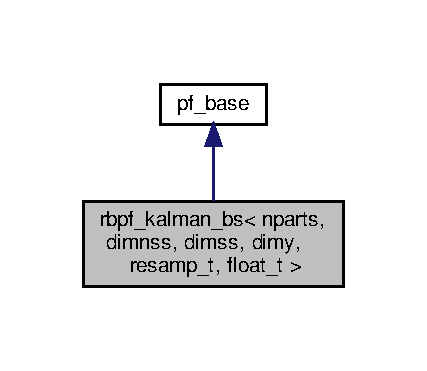
\includegraphics[width=205pt]{classrbpf__kalman__bs__inherit__graph}
\end{center}
\end{figure}


Collaboration diagram for rbpf\+\_\+kalman\+\_\+bs$<$ nparts, dimnss, dimss, dimy, resamp\+\_\+t, float\+\_\+t $>$\+:
\nopagebreak
\begin{figure}[H]
\begin{center}
\leavevmode
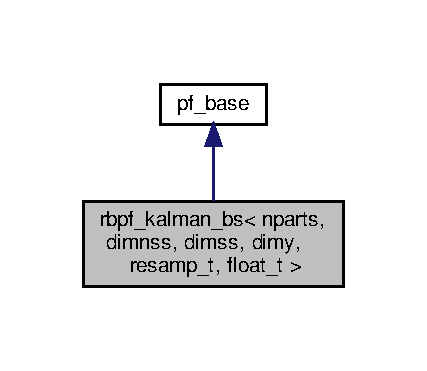
\includegraphics[width=205pt]{classrbpf__kalman__bs__coll__graph}
\end{center}
\end{figure}
\subsection*{Public Types}
\begin{DoxyCompactItemize}
\item 
using \hyperlink{classrbpf__kalman__bs_a2b40c9fa0d7a2ca42be3d0c43db0db8b}{sssv} = Eigen\+::\+Matrix$<$ float\+\_\+t, dimss, 1 $>$
\item 
using \hyperlink{classrbpf__kalman__bs_a896c6ca25182e5569df4bfa6c40f9a54}{nsssv} = Eigen\+::\+Matrix$<$ float\+\_\+t, dimnss, 1 $>$
\item 
using \hyperlink{classrbpf__kalman__bs_a51f159fe3b1d23742ba06d82d4724186}{osv} = Eigen\+::\+Matrix$<$ float\+\_\+t, dimy, 1 $>$
\item 
using \hyperlink{classrbpf__kalman__bs_add5db33a27f25ec3e72ecd8e4c9ce755}{Mat} = Eigen\+::\+Matrix$<$ float\+\_\+t, Eigen\+::\+Dynamic, Eigen\+::\+Dynamic $>$
\item 
using \hyperlink{classrbpf__kalman__bs_a0d3dfd24b849c0bf33fa3df8ce56dd07}{nsss\+Mat} = Eigen\+::\+Matrix$<$ float\+\_\+t, dimnss, dimnss $>$
\item 
using \hyperlink{classrbpf__kalman__bs_a009e7dcc39c6a256a6de6ce36df7d033}{array\+Mod} = std\+::array$<$ \hyperlink{classkalman}{kalman}$<$ dimnss, dimy, 0, float\+\_\+t $>$, nparts $>$
\item 
using \hyperlink{classrbpf__kalman__bs_ae4f4df4fb0cffea207901b0d358a519b}{array\+Vec} = std\+::array$<$ \hyperlink{classrbpf__kalman__bs_a2b40c9fa0d7a2ca42be3d0c43db0db8b}{sssv}, nparts $>$
\item 
using \hyperlink{classrbpf__kalman__bs_ae45e5522570234a1126f28fbe6a13c75}{arrayfloat\+\_\+t} = std\+::array$<$ float\+\_\+t, nparts $>$
\end{DoxyCompactItemize}
\subsection*{Public Member Functions}
\begin{DoxyCompactItemize}
\item 
\hyperlink{classrbpf__kalman__bs_afbd99010c2198c6153bfaf9f11a50299}{rbpf\+\_\+kalman\+\_\+bs} (const unsigned int \&resamp\+\_\+sched=1)
\begin{DoxyCompactList}\small\item\em The constructor. \end{DoxyCompactList}\item 
\mbox{\Hypertarget{classrbpf__kalman__bs_af065083e1bea86180b650e4f280cf2b0}\label{classrbpf__kalman__bs_af065083e1bea86180b650e4f280cf2b0}} 
virtual \hyperlink{classrbpf__kalman__bs_af065083e1bea86180b650e4f280cf2b0}{$\sim$rbpf\+\_\+kalman\+\_\+bs} ()
\begin{DoxyCompactList}\small\item\em The (virtual) destructor. \end{DoxyCompactList}\item 
void \hyperlink{classrbpf__kalman__bs_a241e90ba673be5398f17eccc52b727bf}{filter} (const \hyperlink{classrbpf__kalman__bs_a51f159fe3b1d23742ba06d82d4724186}{osv} \&data, const std\+::vector$<$ std\+::function$<$ const \hyperlink{classrbpf__kalman__bs_add5db33a27f25ec3e72ecd8e4c9ce755}{Mat}(const \hyperlink{classrbpf__kalman__bs_a896c6ca25182e5569df4bfa6c40f9a54}{nsssv} \&x1t, const \hyperlink{classrbpf__kalman__bs_a2b40c9fa0d7a2ca42be3d0c43db0db8b}{sssv} \&x2t)$>$ $>$ \&fs=std\+::vector$<$ std\+::function$<$ const \hyperlink{classrbpf__kalman__bs_add5db33a27f25ec3e72ecd8e4c9ce755}{Mat}(const \hyperlink{classrbpf__kalman__bs_a896c6ca25182e5569df4bfa6c40f9a54}{nsssv} \&x1t, const \hyperlink{classrbpf__kalman__bs_a2b40c9fa0d7a2ca42be3d0c43db0db8b}{sssv} \&x2t)$>$ $>$())
\begin{DoxyCompactList}\small\item\em Filter! \end{DoxyCompactList}\item 
float\+\_\+t \hyperlink{classrbpf__kalman__bs_af2ddf0fc3bf89516f3ebc8187b055a57}{get\+Log\+Cond\+Like} () const
\begin{DoxyCompactList}\small\item\em Get the latest log conditional likelihood. \end{DoxyCompactList}\item 
std\+::vector$<$ \hyperlink{classrbpf__kalman__bs_add5db33a27f25ec3e72ecd8e4c9ce755}{Mat} $>$ \hyperlink{classrbpf__kalman__bs_af4874bee4d5ea66fda9c4212b6030af7}{get\+Expectations} () const
\begin{DoxyCompactList}\small\item\em Get the latest filtered expectation E\mbox{[}h(x\+\_\+1t, x\+\_\+2t) $\vert$ y\+\_\+\{1\+:t\}\mbox{]}. \end{DoxyCompactList}\item 
virtual \hyperlink{classrbpf__kalman__bs_a2b40c9fa0d7a2ca42be3d0c43db0db8b}{sssv} \hyperlink{classrbpf__kalman__bs_addafd7af8bf500d23a09aad34bf9cf0b}{mu\+Samp} ()=0
\begin{DoxyCompactList}\small\item\em Sample from the first time\textquotesingle{}s proposal distribution. \end{DoxyCompactList}\item 
virtual \hyperlink{classrbpf__kalman__bs_a896c6ca25182e5569df4bfa6c40f9a54}{nsssv} \hyperlink{classrbpf__kalman__bs_a8bb7a29b1bcc66cfb4ebf86c0d091ec1}{init\+Kalman\+Mean} (const \hyperlink{classrbpf__kalman__bs_a2b40c9fa0d7a2ca42be3d0c43db0db8b}{sssv} \&x21)=0
\begin{DoxyCompactList}\small\item\em Provides the initial mean vector for each Kalman filter object. \end{DoxyCompactList}\item 
virtual \hyperlink{classrbpf__kalman__bs_a0d3dfd24b849c0bf33fa3df8ce56dd07}{nsss\+Mat} \hyperlink{classrbpf__kalman__bs_add33853e65897cc359965d3715e4e20f}{init\+Kalman\+Var} (const \hyperlink{classrbpf__kalman__bs_a2b40c9fa0d7a2ca42be3d0c43db0db8b}{sssv} \&x21)=0
\begin{DoxyCompactList}\small\item\em Provides the initial covariance matrix for each Kalman filter object. \end{DoxyCompactList}\item 
virtual \hyperlink{classrbpf__kalman__bs_a2b40c9fa0d7a2ca42be3d0c43db0db8b}{sssv} \hyperlink{classrbpf__kalman__bs_afce6418525aea80ea8f073eda77bb6f4}{f\+Samp} (const \hyperlink{classrbpf__kalman__bs_a2b40c9fa0d7a2ca42be3d0c43db0db8b}{sssv} \&x2tm1)=0
\begin{DoxyCompactList}\small\item\em Samples the time t second component. \end{DoxyCompactList}\item 
virtual void \hyperlink{classrbpf__kalman__bs_a3a382531f3af3856735ce031e34a5f54}{update\+Kalman} (\hyperlink{classkalman}{kalman}$<$ dimnss, dimy, 0, float\+\_\+t $>$ \&k\+Mod, const \hyperlink{classrbpf__kalman__bs_a51f159fe3b1d23742ba06d82d4724186}{osv} \&yt, const \hyperlink{classrbpf__kalman__bs_a2b40c9fa0d7a2ca42be3d0c43db0db8b}{sssv} \&x2t)=0
\begin{DoxyCompactList}\small\item\em How to update your inner Kalman filter object at each time. \end{DoxyCompactList}\end{DoxyCompactItemize}
\subsection*{Private Attributes}
\begin{DoxyCompactItemize}
\item 
unsigned int \hyperlink{classrbpf__kalman__bs_a0d8b3393bb7cb301a6719e56d2c646a9}{m\+\_\+rs}
\item 
\hyperlink{classrbpf__kalman__bs_a009e7dcc39c6a256a6de6ce36df7d033}{array\+Mod} \hyperlink{classrbpf__kalman__bs_a15975ae1d3e70b7bac82f09139d07250}{m\+\_\+p\+\_\+inner\+Mods}
\item 
\hyperlink{classrbpf__kalman__bs_ae4f4df4fb0cffea207901b0d358a519b}{array\+Vec} \hyperlink{classrbpf__kalman__bs_a301e07b418473f266af0b4ad05e82a04}{m\+\_\+p\+\_\+samps}
\item 
\hyperlink{classrbpf__kalman__bs_ae45e5522570234a1126f28fbe6a13c75}{arrayfloat\+\_\+t} \hyperlink{classrbpf__kalman__bs_a2f61f3dca55d4c7f32b408569a75f464}{m\+\_\+log\+Un\+Norm\+Weights}
\item 
unsigned int \hyperlink{classrbpf__kalman__bs_a84dfd5c00db5f3772430498585b776d6}{m\+\_\+now}
\item 
float\+\_\+t \hyperlink{classrbpf__kalman__bs_afb9c933b188a5bb70a35ab404515bde2}{m\+\_\+last\+Log\+Cond\+Like}
\item 
resamp\+\_\+t \hyperlink{classrbpf__kalman__bs_a9ec4d8c343bb45953ef2eac0e0e3210b}{m\+\_\+resampler}
\item 
std\+::vector$<$ \hyperlink{classrbpf__kalman__bs_add5db33a27f25ec3e72ecd8e4c9ce755}{Mat} $>$ \hyperlink{classrbpf__kalman__bs_abf448200e8922c6efa03d18b58712a39}{m\+\_\+expectations}
\end{DoxyCompactItemize}


\subsection{Detailed Description}
\subsubsection*{template$<$size\+\_\+t nparts, size\+\_\+t dimnss, size\+\_\+t dimss, size\+\_\+t dimy, typename resamp\+\_\+t, typename float\+\_\+t$>$\newline
class rbpf\+\_\+kalman\+\_\+bs$<$ nparts, dimnss, dimss, dimy, resamp\+\_\+t, float\+\_\+t $>$}

Rao-\/\+Blackwellized/\+Marginal Bootstrap Filter with inner Kalman Filter objectss. 

\begin{DoxyAuthor}{Author}
t 
\end{DoxyAuthor}


\subsection{Member Typedef Documentation}
\mbox{\Hypertarget{classrbpf__kalman__bs_ae45e5522570234a1126f28fbe6a13c75}\label{classrbpf__kalman__bs_ae45e5522570234a1126f28fbe6a13c75}} 
\index{rbpf\+\_\+kalman\+\_\+bs@{rbpf\+\_\+kalman\+\_\+bs}!arrayfloat\+\_\+t@{arrayfloat\+\_\+t}}
\index{arrayfloat\+\_\+t@{arrayfloat\+\_\+t}!rbpf\+\_\+kalman\+\_\+bs@{rbpf\+\_\+kalman\+\_\+bs}}
\subsubsection{\texorpdfstring{arrayfloat\+\_\+t}{arrayfloat\_t}}
{\footnotesize\ttfamily template$<$size\+\_\+t nparts, size\+\_\+t dimnss, size\+\_\+t dimss, size\+\_\+t dimy, typename resamp\+\_\+t , typename float\+\_\+t $>$ \\
using \hyperlink{classrbpf__kalman__bs}{rbpf\+\_\+kalman\+\_\+bs}$<$ nparts, dimnss, dimss, dimy, resamp\+\_\+t, float\+\_\+t $>$\+::\hyperlink{classrbpf__kalman__bs_ae45e5522570234a1126f28fbe6a13c75}{arrayfloat\+\_\+t} =  std\+::array$<$float\+\_\+t,nparts$>$}

array of weights \mbox{\Hypertarget{classrbpf__kalman__bs_a009e7dcc39c6a256a6de6ce36df7d033}\label{classrbpf__kalman__bs_a009e7dcc39c6a256a6de6ce36df7d033}} 
\index{rbpf\+\_\+kalman\+\_\+bs@{rbpf\+\_\+kalman\+\_\+bs}!array\+Mod@{array\+Mod}}
\index{array\+Mod@{array\+Mod}!rbpf\+\_\+kalman\+\_\+bs@{rbpf\+\_\+kalman\+\_\+bs}}
\subsubsection{\texorpdfstring{array\+Mod}{arrayMod}}
{\footnotesize\ttfamily template$<$size\+\_\+t nparts, size\+\_\+t dimnss, size\+\_\+t dimss, size\+\_\+t dimy, typename resamp\+\_\+t , typename float\+\_\+t $>$ \\
using \hyperlink{classrbpf__kalman__bs}{rbpf\+\_\+kalman\+\_\+bs}$<$ nparts, dimnss, dimss, dimy, resamp\+\_\+t, float\+\_\+t $>$\+::\hyperlink{classrbpf__kalman__bs_a009e7dcc39c6a256a6de6ce36df7d033}{array\+Mod} =  std\+::array$<$\hyperlink{classkalman}{kalman}$<$dimnss,dimy,0,float\+\_\+t$>$,nparts$>$}

array of model objects \mbox{\Hypertarget{classrbpf__kalman__bs_ae4f4df4fb0cffea207901b0d358a519b}\label{classrbpf__kalman__bs_ae4f4df4fb0cffea207901b0d358a519b}} 
\index{rbpf\+\_\+kalman\+\_\+bs@{rbpf\+\_\+kalman\+\_\+bs}!array\+Vec@{array\+Vec}}
\index{array\+Vec@{array\+Vec}!rbpf\+\_\+kalman\+\_\+bs@{rbpf\+\_\+kalman\+\_\+bs}}
\subsubsection{\texorpdfstring{array\+Vec}{arrayVec}}
{\footnotesize\ttfamily template$<$size\+\_\+t nparts, size\+\_\+t dimnss, size\+\_\+t dimss, size\+\_\+t dimy, typename resamp\+\_\+t , typename float\+\_\+t $>$ \\
using \hyperlink{classrbpf__kalman__bs}{rbpf\+\_\+kalman\+\_\+bs}$<$ nparts, dimnss, dimss, dimy, resamp\+\_\+t, float\+\_\+t $>$\+::\hyperlink{classrbpf__kalman__bs_ae4f4df4fb0cffea207901b0d358a519b}{array\+Vec} =  std\+::array$<$\hyperlink{classrbpf__kalman__bs_a2b40c9fa0d7a2ca42be3d0c43db0db8b}{sssv},nparts$>$}

array of samples \mbox{\Hypertarget{classrbpf__kalman__bs_add5db33a27f25ec3e72ecd8e4c9ce755}\label{classrbpf__kalman__bs_add5db33a27f25ec3e72ecd8e4c9ce755}} 
\index{rbpf\+\_\+kalman\+\_\+bs@{rbpf\+\_\+kalman\+\_\+bs}!Mat@{Mat}}
\index{Mat@{Mat}!rbpf\+\_\+kalman\+\_\+bs@{rbpf\+\_\+kalman\+\_\+bs}}
\subsubsection{\texorpdfstring{Mat}{Mat}}
{\footnotesize\ttfamily template$<$size\+\_\+t nparts, size\+\_\+t dimnss, size\+\_\+t dimss, size\+\_\+t dimy, typename resamp\+\_\+t , typename float\+\_\+t $>$ \\
using \hyperlink{classrbpf__kalman__bs}{rbpf\+\_\+kalman\+\_\+bs}$<$ nparts, dimnss, dimss, dimy, resamp\+\_\+t, float\+\_\+t $>$\+::\hyperlink{classrbpf__kalman__bs_add5db33a27f25ec3e72ecd8e4c9ce755}{Mat} =  Eigen\+::\+Matrix$<$float\+\_\+t,Eigen\+::\+Dynamic,Eigen\+::\+Dynamic$>$}

dynamic size matrices \mbox{\Hypertarget{classrbpf__kalman__bs_a0d3dfd24b849c0bf33fa3df8ce56dd07}\label{classrbpf__kalman__bs_a0d3dfd24b849c0bf33fa3df8ce56dd07}} 
\index{rbpf\+\_\+kalman\+\_\+bs@{rbpf\+\_\+kalman\+\_\+bs}!nsss\+Mat@{nsss\+Mat}}
\index{nsss\+Mat@{nsss\+Mat}!rbpf\+\_\+kalman\+\_\+bs@{rbpf\+\_\+kalman\+\_\+bs}}
\subsubsection{\texorpdfstring{nsss\+Mat}{nsssMat}}
{\footnotesize\ttfamily template$<$size\+\_\+t nparts, size\+\_\+t dimnss, size\+\_\+t dimss, size\+\_\+t dimy, typename resamp\+\_\+t , typename float\+\_\+t $>$ \\
using \hyperlink{classrbpf__kalman__bs}{rbpf\+\_\+kalman\+\_\+bs}$<$ nparts, dimnss, dimss, dimy, resamp\+\_\+t, float\+\_\+t $>$\+::\hyperlink{classrbpf__kalman__bs_a0d3dfd24b849c0bf33fa3df8ce56dd07}{nsss\+Mat} =  Eigen\+::\+Matrix$<$float\+\_\+t,dimnss,dimnss$>$}

\char`\"{}not sampled state size matrix\char`\"{} \mbox{\Hypertarget{classrbpf__kalman__bs_a896c6ca25182e5569df4bfa6c40f9a54}\label{classrbpf__kalman__bs_a896c6ca25182e5569df4bfa6c40f9a54}} 
\index{rbpf\+\_\+kalman\+\_\+bs@{rbpf\+\_\+kalman\+\_\+bs}!nsssv@{nsssv}}
\index{nsssv@{nsssv}!rbpf\+\_\+kalman\+\_\+bs@{rbpf\+\_\+kalman\+\_\+bs}}
\subsubsection{\texorpdfstring{nsssv}{nsssv}}
{\footnotesize\ttfamily template$<$size\+\_\+t nparts, size\+\_\+t dimnss, size\+\_\+t dimss, size\+\_\+t dimy, typename resamp\+\_\+t , typename float\+\_\+t $>$ \\
using \hyperlink{classrbpf__kalman__bs}{rbpf\+\_\+kalman\+\_\+bs}$<$ nparts, dimnss, dimss, dimy, resamp\+\_\+t, float\+\_\+t $>$\+::\hyperlink{classrbpf__kalman__bs_a896c6ca25182e5569df4bfa6c40f9a54}{nsssv} =  Eigen\+::\+Matrix$<$float\+\_\+t,dimnss,1$>$}

\char`\"{}not sampled state size vector\char`\"{} \mbox{\Hypertarget{classrbpf__kalman__bs_a51f159fe3b1d23742ba06d82d4724186}\label{classrbpf__kalman__bs_a51f159fe3b1d23742ba06d82d4724186}} 
\index{rbpf\+\_\+kalman\+\_\+bs@{rbpf\+\_\+kalman\+\_\+bs}!osv@{osv}}
\index{osv@{osv}!rbpf\+\_\+kalman\+\_\+bs@{rbpf\+\_\+kalman\+\_\+bs}}
\subsubsection{\texorpdfstring{osv}{osv}}
{\footnotesize\ttfamily template$<$size\+\_\+t nparts, size\+\_\+t dimnss, size\+\_\+t dimss, size\+\_\+t dimy, typename resamp\+\_\+t , typename float\+\_\+t $>$ \\
using \hyperlink{classrbpf__kalman__bs}{rbpf\+\_\+kalman\+\_\+bs}$<$ nparts, dimnss, dimss, dimy, resamp\+\_\+t, float\+\_\+t $>$\+::\hyperlink{classrbpf__kalman__bs_a51f159fe3b1d23742ba06d82d4724186}{osv} =  Eigen\+::\+Matrix$<$float\+\_\+t,dimy,1$>$}

\char`\"{}observation size vector\char`\"{} \mbox{\Hypertarget{classrbpf__kalman__bs_a2b40c9fa0d7a2ca42be3d0c43db0db8b}\label{classrbpf__kalman__bs_a2b40c9fa0d7a2ca42be3d0c43db0db8b}} 
\index{rbpf\+\_\+kalman\+\_\+bs@{rbpf\+\_\+kalman\+\_\+bs}!sssv@{sssv}}
\index{sssv@{sssv}!rbpf\+\_\+kalman\+\_\+bs@{rbpf\+\_\+kalman\+\_\+bs}}
\subsubsection{\texorpdfstring{sssv}{sssv}}
{\footnotesize\ttfamily template$<$size\+\_\+t nparts, size\+\_\+t dimnss, size\+\_\+t dimss, size\+\_\+t dimy, typename resamp\+\_\+t , typename float\+\_\+t $>$ \\
using \hyperlink{classrbpf__kalman__bs}{rbpf\+\_\+kalman\+\_\+bs}$<$ nparts, dimnss, dimss, dimy, resamp\+\_\+t, float\+\_\+t $>$\+::\hyperlink{classrbpf__kalman__bs_a2b40c9fa0d7a2ca42be3d0c43db0db8b}{sssv} =  Eigen\+::\+Matrix$<$float\+\_\+t,dimss,1$>$}

\char`\"{}sampled state size vector\char`\"{} 

\subsection{Constructor \& Destructor Documentation}
\mbox{\Hypertarget{classrbpf__kalman__bs_afbd99010c2198c6153bfaf9f11a50299}\label{classrbpf__kalman__bs_afbd99010c2198c6153bfaf9f11a50299}} 
\index{rbpf\+\_\+kalman\+\_\+bs@{rbpf\+\_\+kalman\+\_\+bs}!rbpf\+\_\+kalman\+\_\+bs@{rbpf\+\_\+kalman\+\_\+bs}}
\index{rbpf\+\_\+kalman\+\_\+bs@{rbpf\+\_\+kalman\+\_\+bs}!rbpf\+\_\+kalman\+\_\+bs@{rbpf\+\_\+kalman\+\_\+bs}}
\subsubsection{\texorpdfstring{rbpf\+\_\+kalman\+\_\+bs()}{rbpf\_kalman\_bs()}}
{\footnotesize\ttfamily template$<$size\+\_\+t nparts, size\+\_\+t dimnss, size\+\_\+t dimss, size\+\_\+t dimy, typename resamp\+\_\+t , typename float\+\_\+t $>$ \\
\hyperlink{classrbpf__kalman__bs}{rbpf\+\_\+kalman\+\_\+bs}$<$ nparts, dimnss, dimss, dimy, resamp\+\_\+t, float\+\_\+t $>$\+::\hyperlink{classrbpf__kalman__bs}{rbpf\+\_\+kalman\+\_\+bs} (\begin{DoxyParamCaption}\item[{const unsigned int \&}]{resamp\+\_\+sched = {\ttfamily 1} }\end{DoxyParamCaption})}



The constructor. 


\begin{DoxyParams}{Parameters}
{\em resamp\+\_\+sched} & how often you want to resample (e.\+g once every resamp\+\_\+sched time points) \\
\hline
\end{DoxyParams}


\subsection{Member Function Documentation}
\mbox{\Hypertarget{classrbpf__kalman__bs_a241e90ba673be5398f17eccc52b727bf}\label{classrbpf__kalman__bs_a241e90ba673be5398f17eccc52b727bf}} 
\index{rbpf\+\_\+kalman\+\_\+bs@{rbpf\+\_\+kalman\+\_\+bs}!filter@{filter}}
\index{filter@{filter}!rbpf\+\_\+kalman\+\_\+bs@{rbpf\+\_\+kalman\+\_\+bs}}
\subsubsection{\texorpdfstring{filter()}{filter()}}
{\footnotesize\ttfamily template$<$size\+\_\+t nparts, size\+\_\+t dimnss, size\+\_\+t dimss, size\+\_\+t dimy, typename resamp\+\_\+t , typename float\+\_\+t $>$ \\
void \hyperlink{classrbpf__kalman__bs}{rbpf\+\_\+kalman\+\_\+bs}$<$ nparts, dimnss, dimss, dimy, resamp\+\_\+t, float\+\_\+t $>$\+::filter (\begin{DoxyParamCaption}\item[{const \hyperlink{classrbpf__kalman__bs_a51f159fe3b1d23742ba06d82d4724186}{osv} \&}]{data,  }\item[{const std\+::vector$<$ std\+::function$<$ const \hyperlink{classrbpf__kalman__bs_add5db33a27f25ec3e72ecd8e4c9ce755}{Mat}(const \hyperlink{classrbpf__kalman__bs_a896c6ca25182e5569df4bfa6c40f9a54}{nsssv} \&x1t, const \hyperlink{classrbpf__kalman__bs_a2b40c9fa0d7a2ca42be3d0c43db0db8b}{sssv} \&x2t)$>$ $>$ \&}]{fs = {\ttfamily std\+:\+:vector$<$std\+:\+:function$<$const~\hyperlink{classrbpf__kalman__bs_add5db33a27f25ec3e72ecd8e4c9ce755}{Mat}(const~\hyperlink{classrbpf__kalman__bs_a896c6ca25182e5569df4bfa6c40f9a54}{nsssv}~\&x1t,~const~\hyperlink{classrbpf__kalman__bs_a2b40c9fa0d7a2ca42be3d0c43db0db8b}{sssv}~\&x2t)$>$~$>$()} }\end{DoxyParamCaption})}



Filter! 

The workhorse function 
\begin{DoxyParams}{Parameters}
{\em data} & the most recent observable portion of the time series. \\
\hline
{\em fs} & a vector of functions computing E\mbox{[}h(x\+\_\+1t, x\+\_\+2t$^\wedge$i)$\vert$ x\+\_\+2t$^\wedge$i,y\+\_\+1\+:t\mbox{]}. to be averaged to yield E\mbox{[}h(x\+\_\+1t, x\+\_\+2t)$\vert$,y\+\_\+1\+:t\mbox{]} \\
\hline
\end{DoxyParams}
\mbox{\Hypertarget{classrbpf__kalman__bs_afce6418525aea80ea8f073eda77bb6f4}\label{classrbpf__kalman__bs_afce6418525aea80ea8f073eda77bb6f4}} 
\index{rbpf\+\_\+kalman\+\_\+bs@{rbpf\+\_\+kalman\+\_\+bs}!f\+Samp@{f\+Samp}}
\index{f\+Samp@{f\+Samp}!rbpf\+\_\+kalman\+\_\+bs@{rbpf\+\_\+kalman\+\_\+bs}}
\subsubsection{\texorpdfstring{f\+Samp()}{fSamp()}}
{\footnotesize\ttfamily template$<$size\+\_\+t nparts, size\+\_\+t dimnss, size\+\_\+t dimss, size\+\_\+t dimy, typename resamp\+\_\+t , typename float\+\_\+t $>$ \\
virtual \hyperlink{classrbpf__kalman__bs_a2b40c9fa0d7a2ca42be3d0c43db0db8b}{sssv} \hyperlink{classrbpf__kalman__bs}{rbpf\+\_\+kalman\+\_\+bs}$<$ nparts, dimnss, dimss, dimy, resamp\+\_\+t, float\+\_\+t $>$\+::f\+Samp (\begin{DoxyParamCaption}\item[{const \hyperlink{classrbpf__kalman__bs_a2b40c9fa0d7a2ca42be3d0c43db0db8b}{sssv} \&}]{x2tm1 }\end{DoxyParamCaption})\hspace{0.3cm}{\ttfamily [pure virtual]}}



Samples the time t second component. 

Samples the time t second component. 
\begin{DoxyParams}{Parameters}
{\em x2tm1} & the previous time\textquotesingle{}s second state component. \\
\hline
\end{DoxyParams}
\begin{DoxyReturn}{Returns}
a sssv sample of the second state component at the current time. 
\end{DoxyReturn}
\mbox{\Hypertarget{classrbpf__kalman__bs_af4874bee4d5ea66fda9c4212b6030af7}\label{classrbpf__kalman__bs_af4874bee4d5ea66fda9c4212b6030af7}} 
\index{rbpf\+\_\+kalman\+\_\+bs@{rbpf\+\_\+kalman\+\_\+bs}!get\+Expectations@{get\+Expectations}}
\index{get\+Expectations@{get\+Expectations}!rbpf\+\_\+kalman\+\_\+bs@{rbpf\+\_\+kalman\+\_\+bs}}
\subsubsection{\texorpdfstring{get\+Expectations()}{getExpectations()}}
{\footnotesize\ttfamily template$<$size\+\_\+t nparts, size\+\_\+t dimnss, size\+\_\+t dimss, size\+\_\+t dimy, typename resamp\+\_\+t , typename float\+\_\+t $>$ \\
auto \hyperlink{classrbpf__kalman__bs}{rbpf\+\_\+kalman\+\_\+bs}$<$ nparts, dimnss, dimss, dimy, resamp\+\_\+t, float\+\_\+t $>$\+::get\+Expectations (\begin{DoxyParamCaption}{ }\end{DoxyParamCaption}) const}



Get the latest filtered expectation E\mbox{[}h(x\+\_\+1t, x\+\_\+2t) $\vert$ y\+\_\+\{1\+:t\}\mbox{]}. 

Get the expectations you\textquotesingle{}re keeping track of. \begin{DoxyReturn}{Returns}
a vector of Mats 
\end{DoxyReturn}
\mbox{\Hypertarget{classrbpf__kalman__bs_af2ddf0fc3bf89516f3ebc8187b055a57}\label{classrbpf__kalman__bs_af2ddf0fc3bf89516f3ebc8187b055a57}} 
\index{rbpf\+\_\+kalman\+\_\+bs@{rbpf\+\_\+kalman\+\_\+bs}!get\+Log\+Cond\+Like@{get\+Log\+Cond\+Like}}
\index{get\+Log\+Cond\+Like@{get\+Log\+Cond\+Like}!rbpf\+\_\+kalman\+\_\+bs@{rbpf\+\_\+kalman\+\_\+bs}}
\subsubsection{\texorpdfstring{get\+Log\+Cond\+Like()}{getLogCondLike()}}
{\footnotesize\ttfamily template$<$size\+\_\+t nparts, size\+\_\+t dimnss, size\+\_\+t dimss, size\+\_\+t dimy, typename resamp\+\_\+t , typename float\+\_\+t $>$ \\
float\+\_\+t \hyperlink{classrbpf__kalman__bs}{rbpf\+\_\+kalman\+\_\+bs}$<$ nparts, dimnss, dimss, dimy, resamp\+\_\+t, float\+\_\+t $>$\+::get\+Log\+Cond\+Like (\begin{DoxyParamCaption}{ }\end{DoxyParamCaption}) const}



Get the latest log conditional likelihood. 

\begin{DoxyReturn}{Returns}
the latest log conditional likelihood. 
\end{DoxyReturn}
\mbox{\Hypertarget{classrbpf__kalman__bs_a8bb7a29b1bcc66cfb4ebf86c0d091ec1}\label{classrbpf__kalman__bs_a8bb7a29b1bcc66cfb4ebf86c0d091ec1}} 
\index{rbpf\+\_\+kalman\+\_\+bs@{rbpf\+\_\+kalman\+\_\+bs}!init\+Kalman\+Mean@{init\+Kalman\+Mean}}
\index{init\+Kalman\+Mean@{init\+Kalman\+Mean}!rbpf\+\_\+kalman\+\_\+bs@{rbpf\+\_\+kalman\+\_\+bs}}
\subsubsection{\texorpdfstring{init\+Kalman\+Mean()}{initKalmanMean()}}
{\footnotesize\ttfamily template$<$size\+\_\+t nparts, size\+\_\+t dimnss, size\+\_\+t dimss, size\+\_\+t dimy, typename resamp\+\_\+t , typename float\+\_\+t $>$ \\
virtual \hyperlink{classrbpf__kalman__bs_a896c6ca25182e5569df4bfa6c40f9a54}{nsssv} \hyperlink{classrbpf__kalman__bs}{rbpf\+\_\+kalman\+\_\+bs}$<$ nparts, dimnss, dimss, dimy, resamp\+\_\+t, float\+\_\+t $>$\+::init\+Kalman\+Mean (\begin{DoxyParamCaption}\item[{const \hyperlink{classrbpf__kalman__bs_a2b40c9fa0d7a2ca42be3d0c43db0db8b}{sssv} \&}]{x21 }\end{DoxyParamCaption})\hspace{0.3cm}{\ttfamily [pure virtual]}}



Provides the initial mean vector for each Kalman filter object. 

provides the initial mean vector for each Kalman filter object. 
\begin{DoxyParams}{Parameters}
{\em x21} & the second state componenent at time 1. \\
\hline
\end{DoxyParams}
\begin{DoxyReturn}{Returns}
a nsssv representing the unconditional mean. 
\end{DoxyReturn}
\mbox{\Hypertarget{classrbpf__kalman__bs_add33853e65897cc359965d3715e4e20f}\label{classrbpf__kalman__bs_add33853e65897cc359965d3715e4e20f}} 
\index{rbpf\+\_\+kalman\+\_\+bs@{rbpf\+\_\+kalman\+\_\+bs}!init\+Kalman\+Var@{init\+Kalman\+Var}}
\index{init\+Kalman\+Var@{init\+Kalman\+Var}!rbpf\+\_\+kalman\+\_\+bs@{rbpf\+\_\+kalman\+\_\+bs}}
\subsubsection{\texorpdfstring{init\+Kalman\+Var()}{initKalmanVar()}}
{\footnotesize\ttfamily template$<$size\+\_\+t nparts, size\+\_\+t dimnss, size\+\_\+t dimss, size\+\_\+t dimy, typename resamp\+\_\+t , typename float\+\_\+t $>$ \\
virtual \hyperlink{classrbpf__kalman__bs_a0d3dfd24b849c0bf33fa3df8ce56dd07}{nsss\+Mat} \hyperlink{classrbpf__kalman__bs}{rbpf\+\_\+kalman\+\_\+bs}$<$ nparts, dimnss, dimss, dimy, resamp\+\_\+t, float\+\_\+t $>$\+::init\+Kalman\+Var (\begin{DoxyParamCaption}\item[{const \hyperlink{classrbpf__kalman__bs_a2b40c9fa0d7a2ca42be3d0c43db0db8b}{sssv} \&}]{x21 }\end{DoxyParamCaption})\hspace{0.3cm}{\ttfamily [pure virtual]}}



Provides the initial covariance matrix for each Kalman filter object. 

provides the initial covariance matrix for each Kalman filter object. 
\begin{DoxyParams}{Parameters}
{\em x21} & the second state component at time 1. \\
\hline
\end{DoxyParams}
\begin{DoxyReturn}{Returns}
a covariance matrix. 
\end{DoxyReturn}
\mbox{\Hypertarget{classrbpf__kalman__bs_addafd7af8bf500d23a09aad34bf9cf0b}\label{classrbpf__kalman__bs_addafd7af8bf500d23a09aad34bf9cf0b}} 
\index{rbpf\+\_\+kalman\+\_\+bs@{rbpf\+\_\+kalman\+\_\+bs}!mu\+Samp@{mu\+Samp}}
\index{mu\+Samp@{mu\+Samp}!rbpf\+\_\+kalman\+\_\+bs@{rbpf\+\_\+kalman\+\_\+bs}}
\subsubsection{\texorpdfstring{mu\+Samp()}{muSamp()}}
{\footnotesize\ttfamily template$<$size\+\_\+t nparts, size\+\_\+t dimnss, size\+\_\+t dimss, size\+\_\+t dimy, typename resamp\+\_\+t , typename float\+\_\+t $>$ \\
virtual \hyperlink{classrbpf__kalman__bs_a2b40c9fa0d7a2ca42be3d0c43db0db8b}{sssv} \hyperlink{classrbpf__kalman__bs}{rbpf\+\_\+kalman\+\_\+bs}$<$ nparts, dimnss, dimss, dimy, resamp\+\_\+t, float\+\_\+t $>$\+::mu\+Samp (\begin{DoxyParamCaption}{ }\end{DoxyParamCaption})\hspace{0.3cm}{\ttfamily [pure virtual]}}



Sample from the first time\textquotesingle{}s proposal distribution. 

samples the second component of the state at time 1. \begin{DoxyReturn}{Returns}
a sssv sample for x21. 
\end{DoxyReturn}
\mbox{\Hypertarget{classrbpf__kalman__bs_a3a382531f3af3856735ce031e34a5f54}\label{classrbpf__kalman__bs_a3a382531f3af3856735ce031e34a5f54}} 
\index{rbpf\+\_\+kalman\+\_\+bs@{rbpf\+\_\+kalman\+\_\+bs}!update\+Kalman@{update\+Kalman}}
\index{update\+Kalman@{update\+Kalman}!rbpf\+\_\+kalman\+\_\+bs@{rbpf\+\_\+kalman\+\_\+bs}}
\subsubsection{\texorpdfstring{update\+Kalman()}{updateKalman()}}
{\footnotesize\ttfamily template$<$size\+\_\+t nparts, size\+\_\+t dimnss, size\+\_\+t dimss, size\+\_\+t dimy, typename resamp\+\_\+t , typename float\+\_\+t $>$ \\
virtual void \hyperlink{classrbpf__kalman__bs}{rbpf\+\_\+kalman\+\_\+bs}$<$ nparts, dimnss, dimss, dimy, resamp\+\_\+t, float\+\_\+t $>$\+::update\+Kalman (\begin{DoxyParamCaption}\item[{\hyperlink{classkalman}{kalman}$<$ dimnss, dimy, 0, float\+\_\+t $>$ \&}]{k\+Mod,  }\item[{const \hyperlink{classrbpf__kalman__bs_a51f159fe3b1d23742ba06d82d4724186}{osv} \&}]{yt,  }\item[{const \hyperlink{classrbpf__kalman__bs_a2b40c9fa0d7a2ca42be3d0c43db0db8b}{sssv} \&}]{x2t }\end{DoxyParamCaption})\hspace{0.3cm}{\ttfamily [pure virtual]}}



How to update your inner Kalman filter object at each time. 

How to update your inner Kalman filter object at each time. 
\begin{DoxyParams}{Parameters}
{\em k\+Mod} & a Kalman filter object describing the conditional closed-\/form model. \\
\hline
{\em yt} & the current time series observation. \\
\hline
{\em x2t} & the current second state component. \\
\hline
\end{DoxyParams}


\subsection{Member Data Documentation}
\mbox{\Hypertarget{classrbpf__kalman__bs_abf448200e8922c6efa03d18b58712a39}\label{classrbpf__kalman__bs_abf448200e8922c6efa03d18b58712a39}} 
\index{rbpf\+\_\+kalman\+\_\+bs@{rbpf\+\_\+kalman\+\_\+bs}!m\+\_\+expectations@{m\+\_\+expectations}}
\index{m\+\_\+expectations@{m\+\_\+expectations}!rbpf\+\_\+kalman\+\_\+bs@{rbpf\+\_\+kalman\+\_\+bs}}
\subsubsection{\texorpdfstring{m\+\_\+expectations}{m\_expectations}}
{\footnotesize\ttfamily template$<$size\+\_\+t nparts, size\+\_\+t dimnss, size\+\_\+t dimss, size\+\_\+t dimy, typename resamp\+\_\+t , typename float\+\_\+t $>$ \\
std\+::vector$<$\hyperlink{classrbpf__kalman__bs_add5db33a27f25ec3e72ecd8e4c9ce755}{Mat}$>$ \hyperlink{classrbpf__kalman__bs}{rbpf\+\_\+kalman\+\_\+bs}$<$ nparts, dimnss, dimss, dimy, resamp\+\_\+t, float\+\_\+t $>$\+::m\+\_\+expectations\hspace{0.3cm}{\ttfamily [private]}}

expectations \mbox{\Hypertarget{classrbpf__kalman__bs_afb9c933b188a5bb70a35ab404515bde2}\label{classrbpf__kalman__bs_afb9c933b188a5bb70a35ab404515bde2}} 
\index{rbpf\+\_\+kalman\+\_\+bs@{rbpf\+\_\+kalman\+\_\+bs}!m\+\_\+last\+Log\+Cond\+Like@{m\+\_\+last\+Log\+Cond\+Like}}
\index{m\+\_\+last\+Log\+Cond\+Like@{m\+\_\+last\+Log\+Cond\+Like}!rbpf\+\_\+kalman\+\_\+bs@{rbpf\+\_\+kalman\+\_\+bs}}
\subsubsection{\texorpdfstring{m\+\_\+last\+Log\+Cond\+Like}{m\_lastLogCondLike}}
{\footnotesize\ttfamily template$<$size\+\_\+t nparts, size\+\_\+t dimnss, size\+\_\+t dimss, size\+\_\+t dimy, typename resamp\+\_\+t , typename float\+\_\+t $>$ \\
float\+\_\+t \hyperlink{classrbpf__kalman__bs}{rbpf\+\_\+kalman\+\_\+bs}$<$ nparts, dimnss, dimss, dimy, resamp\+\_\+t, float\+\_\+t $>$\+::m\+\_\+last\+Log\+Cond\+Like\hspace{0.3cm}{\ttfamily [private]}}

log p(y\+\_\+t$\vert$y\+\_\+\{1\+:t-\/1\}) or log p(y1) \mbox{\Hypertarget{classrbpf__kalman__bs_a2f61f3dca55d4c7f32b408569a75f464}\label{classrbpf__kalman__bs_a2f61f3dca55d4c7f32b408569a75f464}} 
\index{rbpf\+\_\+kalman\+\_\+bs@{rbpf\+\_\+kalman\+\_\+bs}!m\+\_\+log\+Un\+Norm\+Weights@{m\+\_\+log\+Un\+Norm\+Weights}}
\index{m\+\_\+log\+Un\+Norm\+Weights@{m\+\_\+log\+Un\+Norm\+Weights}!rbpf\+\_\+kalman\+\_\+bs@{rbpf\+\_\+kalman\+\_\+bs}}
\subsubsection{\texorpdfstring{m\+\_\+log\+Un\+Norm\+Weights}{m\_logUnNormWeights}}
{\footnotesize\ttfamily template$<$size\+\_\+t nparts, size\+\_\+t dimnss, size\+\_\+t dimss, size\+\_\+t dimy, typename resamp\+\_\+t , typename float\+\_\+t $>$ \\
\hyperlink{classrbpf__kalman__bs_ae45e5522570234a1126f28fbe6a13c75}{arrayfloat\+\_\+t} \hyperlink{classrbpf__kalman__bs}{rbpf\+\_\+kalman\+\_\+bs}$<$ nparts, dimnss, dimss, dimy, resamp\+\_\+t, float\+\_\+t $>$\+::m\+\_\+log\+Un\+Norm\+Weights\hspace{0.3cm}{\ttfamily [private]}}

the array of the (log of) unnormalized weights \mbox{\Hypertarget{classrbpf__kalman__bs_a84dfd5c00db5f3772430498585b776d6}\label{classrbpf__kalman__bs_a84dfd5c00db5f3772430498585b776d6}} 
\index{rbpf\+\_\+kalman\+\_\+bs@{rbpf\+\_\+kalman\+\_\+bs}!m\+\_\+now@{m\+\_\+now}}
\index{m\+\_\+now@{m\+\_\+now}!rbpf\+\_\+kalman\+\_\+bs@{rbpf\+\_\+kalman\+\_\+bs}}
\subsubsection{\texorpdfstring{m\+\_\+now}{m\_now}}
{\footnotesize\ttfamily template$<$size\+\_\+t nparts, size\+\_\+t dimnss, size\+\_\+t dimss, size\+\_\+t dimy, typename resamp\+\_\+t , typename float\+\_\+t $>$ \\
unsigned int \hyperlink{classrbpf__kalman__bs}{rbpf\+\_\+kalman\+\_\+bs}$<$ nparts, dimnss, dimss, dimy, resamp\+\_\+t, float\+\_\+t $>$\+::m\+\_\+now\hspace{0.3cm}{\ttfamily [private]}}

the current time period \mbox{\Hypertarget{classrbpf__kalman__bs_a15975ae1d3e70b7bac82f09139d07250}\label{classrbpf__kalman__bs_a15975ae1d3e70b7bac82f09139d07250}} 
\index{rbpf\+\_\+kalman\+\_\+bs@{rbpf\+\_\+kalman\+\_\+bs}!m\+\_\+p\+\_\+inner\+Mods@{m\+\_\+p\+\_\+inner\+Mods}}
\index{m\+\_\+p\+\_\+inner\+Mods@{m\+\_\+p\+\_\+inner\+Mods}!rbpf\+\_\+kalman\+\_\+bs@{rbpf\+\_\+kalman\+\_\+bs}}
\subsubsection{\texorpdfstring{m\+\_\+p\+\_\+inner\+Mods}{m\_p\_innerMods}}
{\footnotesize\ttfamily template$<$size\+\_\+t nparts, size\+\_\+t dimnss, size\+\_\+t dimss, size\+\_\+t dimy, typename resamp\+\_\+t , typename float\+\_\+t $>$ \\
\hyperlink{classrbpf__kalman__bs_a009e7dcc39c6a256a6de6ce36df7d033}{array\+Mod} \hyperlink{classrbpf__kalman__bs}{rbpf\+\_\+kalman\+\_\+bs}$<$ nparts, dimnss, dimss, dimy, resamp\+\_\+t, float\+\_\+t $>$\+::m\+\_\+p\+\_\+inner\+Mods\hspace{0.3cm}{\ttfamily [private]}}

the array of inner Kalman filter objects \mbox{\Hypertarget{classrbpf__kalman__bs_a301e07b418473f266af0b4ad05e82a04}\label{classrbpf__kalman__bs_a301e07b418473f266af0b4ad05e82a04}} 
\index{rbpf\+\_\+kalman\+\_\+bs@{rbpf\+\_\+kalman\+\_\+bs}!m\+\_\+p\+\_\+samps@{m\+\_\+p\+\_\+samps}}
\index{m\+\_\+p\+\_\+samps@{m\+\_\+p\+\_\+samps}!rbpf\+\_\+kalman\+\_\+bs@{rbpf\+\_\+kalman\+\_\+bs}}
\subsubsection{\texorpdfstring{m\+\_\+p\+\_\+samps}{m\_p\_samps}}
{\footnotesize\ttfamily template$<$size\+\_\+t nparts, size\+\_\+t dimnss, size\+\_\+t dimss, size\+\_\+t dimy, typename resamp\+\_\+t , typename float\+\_\+t $>$ \\
\hyperlink{classrbpf__kalman__bs_ae4f4df4fb0cffea207901b0d358a519b}{array\+Vec} \hyperlink{classrbpf__kalman__bs}{rbpf\+\_\+kalman\+\_\+bs}$<$ nparts, dimnss, dimss, dimy, resamp\+\_\+t, float\+\_\+t $>$\+::m\+\_\+p\+\_\+samps\hspace{0.3cm}{\ttfamily [private]}}

the array of particle samples \mbox{\Hypertarget{classrbpf__kalman__bs_a9ec4d8c343bb45953ef2eac0e0e3210b}\label{classrbpf__kalman__bs_a9ec4d8c343bb45953ef2eac0e0e3210b}} 
\index{rbpf\+\_\+kalman\+\_\+bs@{rbpf\+\_\+kalman\+\_\+bs}!m\+\_\+resampler@{m\+\_\+resampler}}
\index{m\+\_\+resampler@{m\+\_\+resampler}!rbpf\+\_\+kalman\+\_\+bs@{rbpf\+\_\+kalman\+\_\+bs}}
\subsubsection{\texorpdfstring{m\+\_\+resampler}{m\_resampler}}
{\footnotesize\ttfamily template$<$size\+\_\+t nparts, size\+\_\+t dimnss, size\+\_\+t dimss, size\+\_\+t dimy, typename resamp\+\_\+t , typename float\+\_\+t $>$ \\
resamp\+\_\+t \hyperlink{classrbpf__kalman__bs}{rbpf\+\_\+kalman\+\_\+bs}$<$ nparts, dimnss, dimss, dimy, resamp\+\_\+t, float\+\_\+t $>$\+::m\+\_\+resampler\hspace{0.3cm}{\ttfamily [private]}}

resampler object \mbox{\Hypertarget{classrbpf__kalman__bs_a0d8b3393bb7cb301a6719e56d2c646a9}\label{classrbpf__kalman__bs_a0d8b3393bb7cb301a6719e56d2c646a9}} 
\index{rbpf\+\_\+kalman\+\_\+bs@{rbpf\+\_\+kalman\+\_\+bs}!m\+\_\+rs@{m\+\_\+rs}}
\index{m\+\_\+rs@{m\+\_\+rs}!rbpf\+\_\+kalman\+\_\+bs@{rbpf\+\_\+kalman\+\_\+bs}}
\subsubsection{\texorpdfstring{m\+\_\+rs}{m\_rs}}
{\footnotesize\ttfamily template$<$size\+\_\+t nparts, size\+\_\+t dimnss, size\+\_\+t dimss, size\+\_\+t dimy, typename resamp\+\_\+t , typename float\+\_\+t $>$ \\
unsigned int \hyperlink{classrbpf__kalman__bs}{rbpf\+\_\+kalman\+\_\+bs}$<$ nparts, dimnss, dimss, dimy, resamp\+\_\+t, float\+\_\+t $>$\+::m\+\_\+rs\hspace{0.3cm}{\ttfamily [private]}}

the resamplign schedule 

The documentation for this class was generated from the following file\+:\begin{DoxyCompactItemize}
\item 
include/\hyperlink{rbpf_8h}{rbpf.\+h}\end{DoxyCompactItemize}

\hypertarget{classresid__resampler}{}\section{resid\+\_\+resampler$<$ nparts, dimx, float\+\_\+t $>$ Class Template Reference}
\label{classresid__resampler}\index{resid\+\_\+resampler$<$ nparts, dimx, float\+\_\+t $>$@{resid\+\_\+resampler$<$ nparts, dimx, float\+\_\+t $>$}}


{\ttfamily \#include $<$resamplers.\+h$>$}



Inheritance diagram for resid\+\_\+resampler$<$ nparts, dimx, float\+\_\+t $>$\+:\nopagebreak
\begin{figure}[H]
\begin{center}
\leavevmode
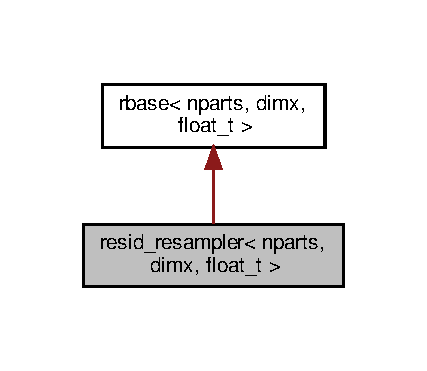
\includegraphics[width=205pt]{classresid__resampler__inherit__graph}
\end{center}
\end{figure}


Collaboration diagram for resid\+\_\+resampler$<$ nparts, dimx, float\+\_\+t $>$\+:\nopagebreak
\begin{figure}[H]
\begin{center}
\leavevmode
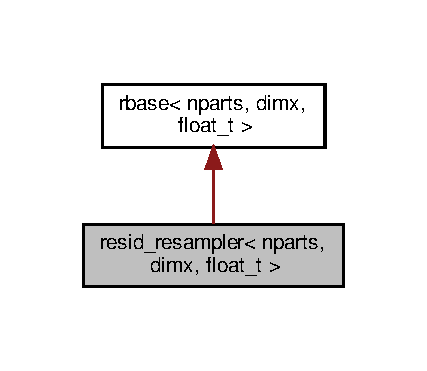
\includegraphics[width=205pt]{classresid__resampler__coll__graph}
\end{center}
\end{figure}
\subsection*{Public Types}
\begin{DoxyCompactItemize}
\item 
using \hyperlink{classresid__resampler_a500f44f0072a4d54b03762c946c38981}{ssv} = Eigen\+::\+Matrix$<$ float\+\_\+t, dimx, 1 $>$
\item 
using \hyperlink{classresid__resampler_a33ba5996cd3099fb81d9932bf5f460c0}{array\+Vec} = std\+::array$<$ \hyperlink{classrbase_ae20e0b8df15aa109252f57ecbf1f20f8}{ssv}, nparts $>$
\item 
using \hyperlink{classresid__resampler_ab95ecc6d5a33f1cbc9089a6b818df405}{array\+Float} = std\+::array$<$ float\+\_\+t, nparts $>$
\item 
using \hyperlink{classresid__resampler_a2ca1138b2d0fcad22c3720c83e56fc47}{array\+Int} = std\+::array$<$ unsigned int, nparts $>$
\end{DoxyCompactItemize}
\subsection*{Public Member Functions}
\begin{DoxyCompactItemize}
\item 
\mbox{\Hypertarget{classresid__resampler_a7b3ebcc490d296b4ad9747c369b92f67}\label{classresid__resampler_a7b3ebcc490d296b4ad9747c369b92f67}} 
\hyperlink{classresid__resampler_a7b3ebcc490d296b4ad9747c369b92f67}{resid\+\_\+resampler} ()=default
\begin{DoxyCompactList}\small\item\em Default constructor. Only option available. \end{DoxyCompactList}\item 
void \hyperlink{classresid__resampler_ae6957cd1e080ac4313e6b0bc5ae9aa96}{resamp\+Log\+Wts} (\hyperlink{classrbase_aa12fc826befa6ba0647b5f59ebc396ee}{array\+Vec} \&old\+Parts, \hyperlink{classrbase_a6f76bef853e508cb5b6f546d231b06f5}{array\+Float} \&old\+Log\+Un\+Norm\+Wts)
\begin{DoxyCompactList}\small\item\em resamples particles. \end{DoxyCompactList}\end{DoxyCompactItemize}
\subsection*{Additional Inherited Members}


\subsection{Detailed Description}
\subsubsection*{template$<$size\+\_\+t nparts, size\+\_\+t dimx, typename float\+\_\+t$>$\newline
class resid\+\_\+resampler$<$ nparts, dimx, float\+\_\+t $>$}

\begin{DoxyAuthor}{Author}
taylor 
\end{DoxyAuthor}
\begin{DoxyDate}{Date}
10/25/19 
\end{DoxyDate}


\subsection{Member Typedef Documentation}
\mbox{\Hypertarget{classresid__resampler_ab95ecc6d5a33f1cbc9089a6b818df405}\label{classresid__resampler_ab95ecc6d5a33f1cbc9089a6b818df405}} 
\index{resid\+\_\+resampler@{resid\+\_\+resampler}!array\+Float@{array\+Float}}
\index{array\+Float@{array\+Float}!resid\+\_\+resampler@{resid\+\_\+resampler}}
\subsubsection{\texorpdfstring{array\+Float}{arrayFloat}}
{\footnotesize\ttfamily template$<$size\+\_\+t nparts, size\+\_\+t dimx, typename float\+\_\+t $>$ \\
using \hyperlink{classresid__resampler}{resid\+\_\+resampler}$<$ nparts, dimx, float\+\_\+t $>$\+::\hyperlink{classrbase_a6f76bef853e508cb5b6f546d231b06f5}{array\+Float} =  std\+::array$<$float\+\_\+t,nparts$>$}

type alias for array of float\+\_\+ts \mbox{\Hypertarget{classresid__resampler_a2ca1138b2d0fcad22c3720c83e56fc47}\label{classresid__resampler_a2ca1138b2d0fcad22c3720c83e56fc47}} 
\index{resid\+\_\+resampler@{resid\+\_\+resampler}!array\+Int@{array\+Int}}
\index{array\+Int@{array\+Int}!resid\+\_\+resampler@{resid\+\_\+resampler}}
\subsubsection{\texorpdfstring{array\+Int}{arrayInt}}
{\footnotesize\ttfamily template$<$size\+\_\+t nparts, size\+\_\+t dimx, typename float\+\_\+t $>$ \\
using \hyperlink{classresid__resampler}{resid\+\_\+resampler}$<$ nparts, dimx, float\+\_\+t $>$\+::\hyperlink{classresid__resampler_a2ca1138b2d0fcad22c3720c83e56fc47}{array\+Int} =  std\+::array$<$unsigned int, nparts$>$}

type alias for array of integers \mbox{\Hypertarget{classresid__resampler_a33ba5996cd3099fb81d9932bf5f460c0}\label{classresid__resampler_a33ba5996cd3099fb81d9932bf5f460c0}} 
\index{resid\+\_\+resampler@{resid\+\_\+resampler}!array\+Vec@{array\+Vec}}
\index{array\+Vec@{array\+Vec}!resid\+\_\+resampler@{resid\+\_\+resampler}}
\subsubsection{\texorpdfstring{array\+Vec}{arrayVec}}
{\footnotesize\ttfamily template$<$size\+\_\+t nparts, size\+\_\+t dimx, typename float\+\_\+t $>$ \\
using \hyperlink{classresid__resampler}{resid\+\_\+resampler}$<$ nparts, dimx, float\+\_\+t $>$\+::\hyperlink{classrbase_aa12fc826befa6ba0647b5f59ebc396ee}{array\+Vec} =  std\+::array$<$\hyperlink{classrbase_ae20e0b8df15aa109252f57ecbf1f20f8}{ssv}, nparts$>$}

type alias for array of Eigen Matrices \mbox{\Hypertarget{classresid__resampler_a500f44f0072a4d54b03762c946c38981}\label{classresid__resampler_a500f44f0072a4d54b03762c946c38981}} 
\index{resid\+\_\+resampler@{resid\+\_\+resampler}!ssv@{ssv}}
\index{ssv@{ssv}!resid\+\_\+resampler@{resid\+\_\+resampler}}
\subsubsection{\texorpdfstring{ssv}{ssv}}
{\footnotesize\ttfamily template$<$size\+\_\+t nparts, size\+\_\+t dimx, typename float\+\_\+t $>$ \\
using \hyperlink{classresid__resampler}{resid\+\_\+resampler}$<$ nparts, dimx, float\+\_\+t $>$\+::\hyperlink{classrbase_ae20e0b8df15aa109252f57ecbf1f20f8}{ssv} =  Eigen\+::\+Matrix$<$float\+\_\+t,dimx,1$>$}

type alias for linear algebra stuff 

\subsection{Member Function Documentation}
\mbox{\Hypertarget{classresid__resampler_ae6957cd1e080ac4313e6b0bc5ae9aa96}\label{classresid__resampler_ae6957cd1e080ac4313e6b0bc5ae9aa96}} 
\index{resid\+\_\+resampler@{resid\+\_\+resampler}!resamp\+Log\+Wts@{resamp\+Log\+Wts}}
\index{resamp\+Log\+Wts@{resamp\+Log\+Wts}!resid\+\_\+resampler@{resid\+\_\+resampler}}
\subsubsection{\texorpdfstring{resamp\+Log\+Wts()}{resampLogWts()}}
{\footnotesize\ttfamily template$<$size\+\_\+t nparts, size\+\_\+t dimx, typename float\+\_\+t $>$ \\
void \hyperlink{classresid__resampler}{resid\+\_\+resampler}$<$ nparts, dimx, float\+\_\+t $>$\+::resamp\+Log\+Wts (\begin{DoxyParamCaption}\item[{\hyperlink{classrbase_aa12fc826befa6ba0647b5f59ebc396ee}{array\+Vec} \&}]{old\+Parts,  }\item[{\hyperlink{classrbase_a6f76bef853e508cb5b6f546d231b06f5}{array\+Float} \&}]{old\+Log\+Un\+Norm\+Wts }\end{DoxyParamCaption})\hspace{0.3cm}{\ttfamily [virtual]}}



resamples particles. 


\begin{DoxyParams}{Parameters}
{\em old\+Parts} & the old particles \\
\hline
{\em old\+Log\+Un\+Norm\+Wts} & the old log unnormalized weights \\
\hline
\end{DoxyParams}


Implements \hyperlink{classrbase_aff0f6f88fd4656e67f5ebc870f10dd44}{rbase$<$ nparts, dimx, float\+\_\+t $>$}.



The documentation for this class was generated from the following file\+:\begin{DoxyCompactItemize}
\item 
include/\hyperlink{resamplers_8h}{resamplers.\+h}\end{DoxyCompactItemize}

\hypertarget{classrvsamp_1_1rvsamp__base}{}\section{rvsamp\+:\+:rvsamp\+\_\+base Class Reference}
\label{classrvsamp_1_1rvsamp__base}\index{rvsamp\+::rvsamp\+\_\+base@{rvsamp\+::rvsamp\+\_\+base}}


Base class for all random variable sampler types. Primary benefit is that it sets the seed for you.  




{\ttfamily \#include $<$rv\+\_\+samp.\+h$>$}



Inheritance diagram for rvsamp\+:\+:rvsamp\+\_\+base\+:
\nopagebreak
\begin{figure}[H]
\begin{center}
\leavevmode
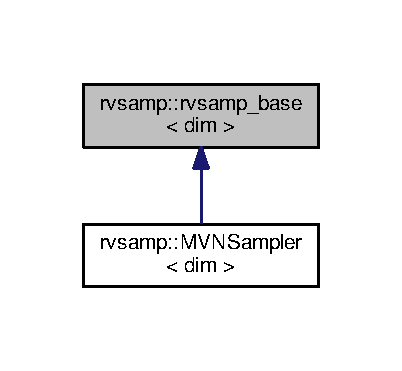
\includegraphics[width=350pt]{classrvsamp_1_1rvsamp__base__inherit__graph}
\end{center}
\end{figure}
\subsection*{Public Member Functions}
\begin{DoxyCompactItemize}
\item 
\mbox{\Hypertarget{classrvsamp_1_1rvsamp__base_ab20e90775a57b9a142520f236b39e7c1}\label{classrvsamp_1_1rvsamp__base_ab20e90775a57b9a142520f236b39e7c1}} 
\hyperlink{classrvsamp_1_1rvsamp__base_ab20e90775a57b9a142520f236b39e7c1}{rvsamp\+\_\+base} ()
\begin{DoxyCompactList}\small\item\em The default constructor. This is the only option available. Sets the seed with the clock. \end{DoxyCompactList}\end{DoxyCompactItemize}
\subsection*{Protected Attributes}
\begin{DoxyCompactItemize}
\item 
\mbox{\Hypertarget{classrvsamp_1_1rvsamp__base_a40eb76e3ecd647c8b1e2d2ef21215dc7}\label{classrvsamp_1_1rvsamp__base_a40eb76e3ecd647c8b1e2d2ef21215dc7}} 
std\+::mt19937 \hyperlink{classrvsamp_1_1rvsamp__base_a40eb76e3ecd647c8b1e2d2ef21215dc7}{m\+\_\+rng}
\begin{DoxyCompactList}\small\item\em prng \end{DoxyCompactList}\end{DoxyCompactItemize}


\subsection{Detailed Description}
Base class for all random variable sampler types. Primary benefit is that it sets the seed for you. 

\begin{DoxyAuthor}{Author}
taylor 
\end{DoxyAuthor}


The documentation for this class was generated from the following file\+:\begin{DoxyCompactItemize}
\item 
include/pf/\hyperlink{rv__samp_8h}{rv\+\_\+samp.\+h}\end{DoxyCompactItemize}

\hypertarget{classSISRFilter}{}\section{S\+I\+S\+R\+Filter$<$ nparts, dimx, dimy, resamp\+\_\+t, float\+\_\+t $>$ Class Template Reference}
\label{classSISRFilter}\index{S\+I\+S\+R\+Filter$<$ nparts, dimx, dimy, resamp\+\_\+t, float\+\_\+t $>$@{S\+I\+S\+R\+Filter$<$ nparts, dimx, dimy, resamp\+\_\+t, float\+\_\+t $>$}}


A base class for the Sequential Important Sampling with Resampling (S\+I\+SR).  




{\ttfamily \#include $<$sisr\+\_\+filter.\+h$>$}



Inheritance diagram for S\+I\+S\+R\+Filter$<$ nparts, dimx, dimy, resamp\+\_\+t, float\+\_\+t $>$\+:\nopagebreak
\begin{figure}[H]
\begin{center}
\leavevmode
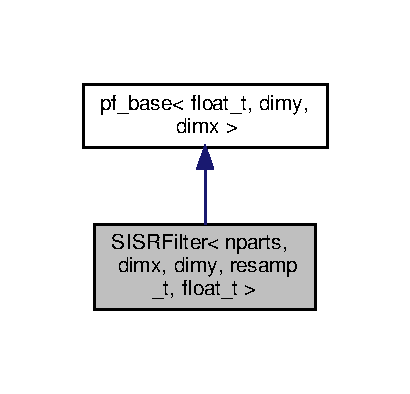
\includegraphics[width=197pt]{classSISRFilter__inherit__graph}
\end{center}
\end{figure}


Collaboration diagram for S\+I\+S\+R\+Filter$<$ nparts, dimx, dimy, resamp\+\_\+t, float\+\_\+t $>$\+:\nopagebreak
\begin{figure}[H]
\begin{center}
\leavevmode
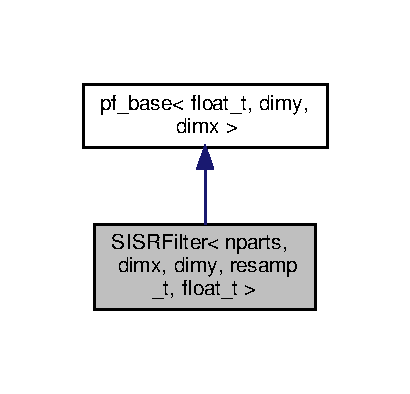
\includegraphics[width=197pt]{classSISRFilter__coll__graph}
\end{center}
\end{figure}
\subsection*{Public Types}
\begin{DoxyCompactItemize}
\item 
using \hyperlink{classSISRFilter_abfec45cf57ea6fadae4a9da8b0042351}{ssv} = Eigen\+::\+Matrix$<$ float\+\_\+t, dimx, 1 $>$
\item 
using \hyperlink{classSISRFilter_a5b762e9352857a9e48db3932191887ef}{osv} = Eigen\+::\+Matrix$<$ float\+\_\+t, dimy, 1 $>$
\item 
using \hyperlink{classSISRFilter_a7355e966778c788dfe227ef5254677c4}{Mat} = Eigen\+::\+Matrix$<$ float\+\_\+t, Eigen\+::\+Dynamic, Eigen\+::\+Dynamic $>$
\item 
using \hyperlink{classSISRFilter_a5c8a38ceb31c22f3c3f38b0ead5c1ce7}{array\+States} = std\+::array$<$ \hyperlink{classSISRFilter_abfec45cf57ea6fadae4a9da8b0042351}{ssv}, nparts $>$
\item 
using \hyperlink{classSISRFilter_a35f5a590324bd78fc4f6ded236937ac2}{arrayfloat\+\_\+t} = std\+::array$<$ float\+\_\+t, nparts $>$
\end{DoxyCompactItemize}
\subsection*{Public Member Functions}
\begin{DoxyCompactItemize}
\item 
\hyperlink{classSISRFilter_a46243d4a5ef93f3762d1130fa4d43389}{S\+I\+S\+R\+Filter} (const unsigned int \&rs=1)
\begin{DoxyCompactList}\small\item\em The (one and only) constructor. \end{DoxyCompactList}\item 
\mbox{\Hypertarget{classSISRFilter_a0934886c2ab47682364e3624c24be874}\label{classSISRFilter_a0934886c2ab47682364e3624c24be874}} 
virtual \hyperlink{classSISRFilter_a0934886c2ab47682364e3624c24be874}{$\sim$\+S\+I\+S\+R\+Filter} ()
\begin{DoxyCompactList}\small\item\em The (virtual) destructor. \end{DoxyCompactList}\item 
float\+\_\+t \hyperlink{classSISRFilter_a48bdb88b2ed4041ab6d8a6547703ebf3}{get\+Log\+Cond\+Like} () const
\begin{DoxyCompactList}\small\item\em Returns the most recent (log-\/) conditiona likelihood. \end{DoxyCompactList}\item 
std\+::vector$<$ \hyperlink{classSISRFilter_a7355e966778c788dfe227ef5254677c4}{Mat} $>$ \hyperlink{classSISRFilter_a88ef9409ded3ec7e6745e184daad86c4}{get\+Expectations} () const
\begin{DoxyCompactList}\small\item\em return all stored expectations (taken with respect to \$p(x\+\_\+t$\vert$y\+\_\+\{1\+:t\})\$ \end{DoxyCompactList}\item 
void \hyperlink{classSISRFilter_a0fd4ac5135ff9a4bb32a286533855197}{filter} (const \hyperlink{classSISRFilter_a5b762e9352857a9e48db3932191887ef}{osv} \&data, const std\+::vector$<$ std\+::function$<$ const \hyperlink{classSISRFilter_a7355e966778c788dfe227ef5254677c4}{Mat}(const \hyperlink{classSISRFilter_abfec45cf57ea6fadae4a9da8b0042351}{ssv} \&)$>$ $>$ \&fs=std\+::vector$<$ std\+::function$<$ const \hyperlink{classSISRFilter_a7355e966778c788dfe227ef5254677c4}{Mat}(const \hyperlink{classSISRFilter_abfec45cf57ea6fadae4a9da8b0042351}{ssv} \&)$>$ $>$())
\begin{DoxyCompactList}\small\item\em updates filtering distribution on a new datapoint. Optionally stores expectations of functionals. \end{DoxyCompactList}\item 
virtual float\+\_\+t \hyperlink{classSISRFilter_aff620e2208b6b26bbe109ce05520c5f8}{log\+Mu\+Ev} (const \hyperlink{classSISRFilter_abfec45cf57ea6fadae4a9da8b0042351}{ssv} \&x1)=0
\begin{DoxyCompactList}\small\item\em Calculate mu\+Ev or logmu\+Ev. \end{DoxyCompactList}\item 
virtual \hyperlink{classSISRFilter_abfec45cf57ea6fadae4a9da8b0042351}{ssv} \hyperlink{classSISRFilter_aac34adbf022dad8b62470de35c5ceb17}{q1\+Samp} (const \hyperlink{classSISRFilter_a5b762e9352857a9e48db3932191887ef}{osv} \&y1)=0
\begin{DoxyCompactList}\small\item\em Samples from time 1 proposal. \end{DoxyCompactList}\item 
virtual float\+\_\+t \hyperlink{classSISRFilter_a21d5130f35d1d5c21b697ca7ea8e9d83}{log\+Q1\+Ev} (const \hyperlink{classSISRFilter_abfec45cf57ea6fadae4a9da8b0042351}{ssv} \&x1, const \hyperlink{classSISRFilter_a5b762e9352857a9e48db3932191887ef}{osv} \&y1)=0
\begin{DoxyCompactList}\small\item\em Calculate q1\+Ev or log q1\+Ev. \end{DoxyCompactList}\item 
virtual float\+\_\+t \hyperlink{classSISRFilter_a73fe8481e4cb40142544c04823851aa8}{log\+G\+Ev} (const \hyperlink{classSISRFilter_a5b762e9352857a9e48db3932191887ef}{osv} \&yt, const \hyperlink{classSISRFilter_abfec45cf57ea6fadae4a9da8b0042351}{ssv} \&xt)=0
\begin{DoxyCompactList}\small\item\em Calculate g\+Ev or log\+G\+Ev. \end{DoxyCompactList}\item 
virtual float\+\_\+t \hyperlink{classSISRFilter_a7aa1e90a0b641728d5f8d7bd8c699ba8}{log\+F\+Ev} (const \hyperlink{classSISRFilter_abfec45cf57ea6fadae4a9da8b0042351}{ssv} \&xt, const \hyperlink{classSISRFilter_abfec45cf57ea6fadae4a9da8b0042351}{ssv} \&xtm1)=0
\begin{DoxyCompactList}\small\item\em Evaluates the state transition density. \end{DoxyCompactList}\item 
virtual \hyperlink{classSISRFilter_abfec45cf57ea6fadae4a9da8b0042351}{ssv} \hyperlink{classSISRFilter_a609bb361da16e1b24ebfab693620241b}{q\+Samp} (const \hyperlink{classSISRFilter_abfec45cf57ea6fadae4a9da8b0042351}{ssv} \&xtm1, const \hyperlink{classSISRFilter_a5b762e9352857a9e48db3932191887ef}{osv} \&yt)=0
\begin{DoxyCompactList}\small\item\em Samples from the proposal/instrumental/importance density at time t. \end{DoxyCompactList}\item 
virtual float\+\_\+t \hyperlink{classSISRFilter_a4edca9291a3a118c37bd0e41c06fb7da}{log\+Q\+Ev} (const \hyperlink{classSISRFilter_abfec45cf57ea6fadae4a9da8b0042351}{ssv} \&xt, const \hyperlink{classSISRFilter_abfec45cf57ea6fadae4a9da8b0042351}{ssv} \&xtm1, const \hyperlink{classSISRFilter_a5b762e9352857a9e48db3932191887ef}{osv} \&yt)=0
\begin{DoxyCompactList}\small\item\em Evaluates the proposal/instrumental/importance density/pmf. \end{DoxyCompactList}\end{DoxyCompactItemize}
\subsection*{Private Attributes}
\begin{DoxyCompactItemize}
\item 
\mbox{\Hypertarget{classSISRFilter_a98c87c50c054354cdc85dc800ba15bdd}\label{classSISRFilter_a98c87c50c054354cdc85dc800ba15bdd}} 
\hyperlink{classSISRFilter_a5c8a38ceb31c22f3c3f38b0ead5c1ce7}{array\+States} \hyperlink{classSISRFilter_a98c87c50c054354cdc85dc800ba15bdd}{m\+\_\+particles}
\begin{DoxyCompactList}\small\item\em particle samples \end{DoxyCompactList}\item 
\mbox{\Hypertarget{classSISRFilter_a99f63cbae203084cf3d812a61bb725fe}\label{classSISRFilter_a99f63cbae203084cf3d812a61bb725fe}} 
\hyperlink{classSISRFilter_a35f5a590324bd78fc4f6ded236937ac2}{arrayfloat\+\_\+t} \hyperlink{classSISRFilter_a99f63cbae203084cf3d812a61bb725fe}{m\+\_\+log\+Un\+Norm\+Weights}
\begin{DoxyCompactList}\small\item\em particle weights \end{DoxyCompactList}\item 
\mbox{\Hypertarget{classSISRFilter_a1aafd7da52826fd25967c8258f68ce9c}\label{classSISRFilter_a1aafd7da52826fd25967c8258f68ce9c}} 
unsigned int \hyperlink{classSISRFilter_a1aafd7da52826fd25967c8258f68ce9c}{m\+\_\+now}
\begin{DoxyCompactList}\small\item\em current time point \end{DoxyCompactList}\item 
\mbox{\Hypertarget{classSISRFilter_a7031db4bd7d9c1db7ea83150893525ed}\label{classSISRFilter_a7031db4bd7d9c1db7ea83150893525ed}} 
float\+\_\+t \hyperlink{classSISRFilter_a7031db4bd7d9c1db7ea83150893525ed}{m\+\_\+log\+Last\+Cond\+Like}
\begin{DoxyCompactList}\small\item\em log p(y\+\_\+t$\vert$y\+\_\+\{1\+:t-\/1\}) or log p(y1) \end{DoxyCompactList}\item 
\mbox{\Hypertarget{classSISRFilter_a46f945e550fab93eedddf10a69c251f1}\label{classSISRFilter_a46f945e550fab93eedddf10a69c251f1}} 
resamp\+\_\+t \hyperlink{classSISRFilter_a46f945e550fab93eedddf10a69c251f1}{m\+\_\+resampler}
\begin{DoxyCompactList}\small\item\em resampling object \end{DoxyCompactList}\item 
\mbox{\Hypertarget{classSISRFilter_acb5ed65aeed970afb929c108d04ee0d1}\label{classSISRFilter_acb5ed65aeed970afb929c108d04ee0d1}} 
std\+::vector$<$ \hyperlink{classSISRFilter_a7355e966778c788dfe227ef5254677c4}{Mat} $>$ \hyperlink{classSISRFilter_acb5ed65aeed970afb929c108d04ee0d1}{m\+\_\+expectations}
\begin{DoxyCompactList}\small\item\em expectations E\mbox{[}h(x\+\_\+t) $\vert$ y\+\_\+\{1\+:t\}\mbox{]} for user defined \char`\"{}h\char`\"{}s \end{DoxyCompactList}\item 
\mbox{\Hypertarget{classSISRFilter_a196049324b4c6c42a927d83f659619aa}\label{classSISRFilter_a196049324b4c6c42a927d83f659619aa}} 
unsigned int \hyperlink{classSISRFilter_a196049324b4c6c42a927d83f659619aa}{m\+\_\+resamp\+Sched}
\begin{DoxyCompactList}\small\item\em resampling schedule (e.\+g. resample every \+\_\+\+\_\+ time points) \end{DoxyCompactList}\end{DoxyCompactItemize}


\subsection{Detailed Description}
\subsubsection*{template$<$size\+\_\+t nparts, size\+\_\+t dimx, size\+\_\+t dimy, typename resamp\+\_\+t, typename float\+\_\+t$>$\newline
class S\+I\+S\+R\+Filter$<$ nparts, dimx, dimy, resamp\+\_\+t, float\+\_\+t $>$}

A base class for the Sequential Important Sampling with Resampling (S\+I\+SR). 

\begin{DoxyAuthor}{Author}
taylor 
\end{DoxyAuthor}


\subsection{Member Typedef Documentation}
\mbox{\Hypertarget{classSISRFilter_a35f5a590324bd78fc4f6ded236937ac2}\label{classSISRFilter_a35f5a590324bd78fc4f6ded236937ac2}} 
\index{S\+I\+S\+R\+Filter@{S\+I\+S\+R\+Filter}!arrayfloat\+\_\+t@{arrayfloat\+\_\+t}}
\index{arrayfloat\+\_\+t@{arrayfloat\+\_\+t}!S\+I\+S\+R\+Filter@{S\+I\+S\+R\+Filter}}
\subsubsection{\texorpdfstring{arrayfloat\+\_\+t}{arrayfloat\_t}}
{\footnotesize\ttfamily template$<$size\+\_\+t nparts, size\+\_\+t dimx, size\+\_\+t dimy, typename resamp\+\_\+t , typename float\+\_\+t $>$ \\
using \hyperlink{classSISRFilter}{S\+I\+S\+R\+Filter}$<$ nparts, dimx, dimy, resamp\+\_\+t, float\+\_\+t $>$\+::\hyperlink{classSISRFilter_a35f5a590324bd78fc4f6ded236937ac2}{arrayfloat\+\_\+t} =  std\+::array$<$float\+\_\+t, nparts$>$}

type alias for array of float\+\_\+ts \mbox{\Hypertarget{classSISRFilter_a5c8a38ceb31c22f3c3f38b0ead5c1ce7}\label{classSISRFilter_a5c8a38ceb31c22f3c3f38b0ead5c1ce7}} 
\index{S\+I\+S\+R\+Filter@{S\+I\+S\+R\+Filter}!array\+States@{array\+States}}
\index{array\+States@{array\+States}!S\+I\+S\+R\+Filter@{S\+I\+S\+R\+Filter}}
\subsubsection{\texorpdfstring{array\+States}{arrayStates}}
{\footnotesize\ttfamily template$<$size\+\_\+t nparts, size\+\_\+t dimx, size\+\_\+t dimy, typename resamp\+\_\+t , typename float\+\_\+t $>$ \\
using \hyperlink{classSISRFilter}{S\+I\+S\+R\+Filter}$<$ nparts, dimx, dimy, resamp\+\_\+t, float\+\_\+t $>$\+::\hyperlink{classSISRFilter_a5c8a38ceb31c22f3c3f38b0ead5c1ce7}{array\+States} =  std\+::array$<$\hyperlink{classSISRFilter_abfec45cf57ea6fadae4a9da8b0042351}{ssv}, nparts$>$}

type alias for linear algebra stuff \mbox{\Hypertarget{classSISRFilter_a7355e966778c788dfe227ef5254677c4}\label{classSISRFilter_a7355e966778c788dfe227ef5254677c4}} 
\index{S\+I\+S\+R\+Filter@{S\+I\+S\+R\+Filter}!Mat@{Mat}}
\index{Mat@{Mat}!S\+I\+S\+R\+Filter@{S\+I\+S\+R\+Filter}}
\subsubsection{\texorpdfstring{Mat}{Mat}}
{\footnotesize\ttfamily template$<$size\+\_\+t nparts, size\+\_\+t dimx, size\+\_\+t dimy, typename resamp\+\_\+t , typename float\+\_\+t $>$ \\
using \hyperlink{classSISRFilter}{S\+I\+S\+R\+Filter}$<$ nparts, dimx, dimy, resamp\+\_\+t, float\+\_\+t $>$\+::\hyperlink{classSISRFilter_a7355e966778c788dfe227ef5254677c4}{Mat} =  Eigen\+::\+Matrix$<$float\+\_\+t,Eigen\+::\+Dynamic,Eigen\+::\+Dynamic$>$}

type alias for linear algebra stuff \mbox{\Hypertarget{classSISRFilter_a5b762e9352857a9e48db3932191887ef}\label{classSISRFilter_a5b762e9352857a9e48db3932191887ef}} 
\index{S\+I\+S\+R\+Filter@{S\+I\+S\+R\+Filter}!osv@{osv}}
\index{osv@{osv}!S\+I\+S\+R\+Filter@{S\+I\+S\+R\+Filter}}
\subsubsection{\texorpdfstring{osv}{osv}}
{\footnotesize\ttfamily template$<$size\+\_\+t nparts, size\+\_\+t dimx, size\+\_\+t dimy, typename resamp\+\_\+t , typename float\+\_\+t $>$ \\
using \hyperlink{classSISRFilter}{S\+I\+S\+R\+Filter}$<$ nparts, dimx, dimy, resamp\+\_\+t, float\+\_\+t $>$\+::\hyperlink{classSISRFilter_a5b762e9352857a9e48db3932191887ef}{osv} =  Eigen\+::\+Matrix$<$float\+\_\+t, dimy, 1$>$}

\char`\"{}obs size vector\char`\"{} type alias for linear algebra stuff \mbox{\Hypertarget{classSISRFilter_abfec45cf57ea6fadae4a9da8b0042351}\label{classSISRFilter_abfec45cf57ea6fadae4a9da8b0042351}} 
\index{S\+I\+S\+R\+Filter@{S\+I\+S\+R\+Filter}!ssv@{ssv}}
\index{ssv@{ssv}!S\+I\+S\+R\+Filter@{S\+I\+S\+R\+Filter}}
\subsubsection{\texorpdfstring{ssv}{ssv}}
{\footnotesize\ttfamily template$<$size\+\_\+t nparts, size\+\_\+t dimx, size\+\_\+t dimy, typename resamp\+\_\+t , typename float\+\_\+t $>$ \\
using \hyperlink{classSISRFilter}{S\+I\+S\+R\+Filter}$<$ nparts, dimx, dimy, resamp\+\_\+t, float\+\_\+t $>$\+::\hyperlink{classSISRFilter_abfec45cf57ea6fadae4a9da8b0042351}{ssv} =  Eigen\+::\+Matrix$<$float\+\_\+t, dimx, 1$>$}

\char`\"{}state size vector\char`\"{} type alias for linear algebra stuff 

\subsection{Constructor \& Destructor Documentation}
\mbox{\Hypertarget{classSISRFilter_a46243d4a5ef93f3762d1130fa4d43389}\label{classSISRFilter_a46243d4a5ef93f3762d1130fa4d43389}} 
\index{S\+I\+S\+R\+Filter@{S\+I\+S\+R\+Filter}!S\+I\+S\+R\+Filter@{S\+I\+S\+R\+Filter}}
\index{S\+I\+S\+R\+Filter@{S\+I\+S\+R\+Filter}!S\+I\+S\+R\+Filter@{S\+I\+S\+R\+Filter}}
\subsubsection{\texorpdfstring{S\+I\+S\+R\+Filter()}{SISRFilter()}}
{\footnotesize\ttfamily template$<$size\+\_\+t nparts, size\+\_\+t dimx, size\+\_\+t dimy, typename resamp\+\_\+t , typename float\+\_\+t $>$ \\
\hyperlink{classSISRFilter}{S\+I\+S\+R\+Filter}$<$ nparts, dimx, dimy, resamp\+\_\+t, float\+\_\+t $>$\+::\hyperlink{classSISRFilter}{S\+I\+S\+R\+Filter} (\begin{DoxyParamCaption}\item[{const unsigned int \&}]{rs = {\ttfamily 1} }\end{DoxyParamCaption})}



The (one and only) constructor. 


\begin{DoxyParams}{Parameters}
{\em rs} & the resampling schedule (resample every rs time points). \\
\hline
\end{DoxyParams}


\subsection{Member Function Documentation}
\mbox{\Hypertarget{classSISRFilter_a0fd4ac5135ff9a4bb32a286533855197}\label{classSISRFilter_a0fd4ac5135ff9a4bb32a286533855197}} 
\index{S\+I\+S\+R\+Filter@{S\+I\+S\+R\+Filter}!filter@{filter}}
\index{filter@{filter}!S\+I\+S\+R\+Filter@{S\+I\+S\+R\+Filter}}
\subsubsection{\texorpdfstring{filter()}{filter()}}
{\footnotesize\ttfamily template$<$size\+\_\+t nparts, size\+\_\+t dimx, size\+\_\+t dimy, typename resamp\+\_\+t , typename float\+\_\+t $>$ \\
void \hyperlink{classSISRFilter}{S\+I\+S\+R\+Filter}$<$ nparts, dimx, dimy, resamp\+\_\+t, float\+\_\+t $>$\+::filter (\begin{DoxyParamCaption}\item[{const \hyperlink{classSISRFilter_a5b762e9352857a9e48db3932191887ef}{osv} \&}]{data,  }\item[{const std\+::vector$<$ std\+::function$<$ const \hyperlink{classSISRFilter_a7355e966778c788dfe227ef5254677c4}{Mat}(const \hyperlink{classSISRFilter_abfec45cf57ea6fadae4a9da8b0042351}{ssv} \&)$>$ $>$ \&}]{fs = {\ttfamily std\+:\+:vector$<$std\+:\+:function$<$const~\hyperlink{classSISRFilter_a7355e966778c788dfe227ef5254677c4}{Mat}(const~\hyperlink{classSISRFilter_abfec45cf57ea6fadae4a9da8b0042351}{ssv}\&)$>$~$>$()} }\end{DoxyParamCaption})}



updates filtering distribution on a new datapoint. Optionally stores expectations of functionals. 


\begin{DoxyParams}{Parameters}
{\em data} & the most recent data point \\
\hline
{\em fs} & a vector of functions if you want to calculate expectations. \\
\hline
\end{DoxyParams}
\mbox{\Hypertarget{classSISRFilter_a88ef9409ded3ec7e6745e184daad86c4}\label{classSISRFilter_a88ef9409ded3ec7e6745e184daad86c4}} 
\index{S\+I\+S\+R\+Filter@{S\+I\+S\+R\+Filter}!get\+Expectations@{get\+Expectations}}
\index{get\+Expectations@{get\+Expectations}!S\+I\+S\+R\+Filter@{S\+I\+S\+R\+Filter}}
\subsubsection{\texorpdfstring{get\+Expectations()}{getExpectations()}}
{\footnotesize\ttfamily template$<$size\+\_\+t nparts, size\+\_\+t dimx, size\+\_\+t dimy, typename resamp\+\_\+t , typename float\+\_\+t $>$ \\
auto \hyperlink{classSISRFilter}{S\+I\+S\+R\+Filter}$<$ nparts, dimx, dimy, resamp\+\_\+t, float\+\_\+t $>$\+::get\+Expectations (\begin{DoxyParamCaption}{ }\end{DoxyParamCaption}) const}



return all stored expectations (taken with respect to \$p(x\+\_\+t$\vert$y\+\_\+\{1\+:t\})\$ 

\begin{DoxyReturn}{Returns}
return a std\+::vector$<$\+Mat$>$ of expectations. How many depends on how many callbacks you gave to 
\end{DoxyReturn}
\mbox{\Hypertarget{classSISRFilter_a48bdb88b2ed4041ab6d8a6547703ebf3}\label{classSISRFilter_a48bdb88b2ed4041ab6d8a6547703ebf3}} 
\index{S\+I\+S\+R\+Filter@{S\+I\+S\+R\+Filter}!get\+Log\+Cond\+Like@{get\+Log\+Cond\+Like}}
\index{get\+Log\+Cond\+Like@{get\+Log\+Cond\+Like}!S\+I\+S\+R\+Filter@{S\+I\+S\+R\+Filter}}
\subsubsection{\texorpdfstring{get\+Log\+Cond\+Like()}{getLogCondLike()}}
{\footnotesize\ttfamily template$<$size\+\_\+t nparts, size\+\_\+t dimx, size\+\_\+t dimy, typename resamp\+\_\+t , typename float\+\_\+t $>$ \\
float\+\_\+t \hyperlink{classSISRFilter}{S\+I\+S\+R\+Filter}$<$ nparts, dimx, dimy, resamp\+\_\+t, float\+\_\+t $>$\+::get\+Log\+Cond\+Like (\begin{DoxyParamCaption}{ }\end{DoxyParamCaption}) const\hspace{0.3cm}{\ttfamily [virtual]}}



Returns the most recent (log-\/) conditiona likelihood. 

\begin{DoxyReturn}{Returns}
log p(y\+\_\+t $\vert$ y\+\_\+\{1\+:t-\/1\}) or log p(y\+\_\+1) 
\end{DoxyReturn}


Implements \hyperlink{classpf__base_a350df818820d6ab0fd6d413022b7f23b}{pf\+\_\+base$<$ float\+\_\+t, dimy, dimx $>$}.

\mbox{\Hypertarget{classSISRFilter_a7aa1e90a0b641728d5f8d7bd8c699ba8}\label{classSISRFilter_a7aa1e90a0b641728d5f8d7bd8c699ba8}} 
\index{S\+I\+S\+R\+Filter@{S\+I\+S\+R\+Filter}!log\+F\+Ev@{log\+F\+Ev}}
\index{log\+F\+Ev@{log\+F\+Ev}!S\+I\+S\+R\+Filter@{S\+I\+S\+R\+Filter}}
\subsubsection{\texorpdfstring{log\+F\+Ev()}{logFEv()}}
{\footnotesize\ttfamily template$<$size\+\_\+t nparts, size\+\_\+t dimx, size\+\_\+t dimy, typename resamp\+\_\+t , typename float\+\_\+t $>$ \\
virtual float\+\_\+t \hyperlink{classSISRFilter}{S\+I\+S\+R\+Filter}$<$ nparts, dimx, dimy, resamp\+\_\+t, float\+\_\+t $>$\+::log\+F\+Ev (\begin{DoxyParamCaption}\item[{const \hyperlink{classSISRFilter_abfec45cf57ea6fadae4a9da8b0042351}{ssv} \&}]{xt,  }\item[{const \hyperlink{classSISRFilter_abfec45cf57ea6fadae4a9da8b0042351}{ssv} \&}]{xtm1 }\end{DoxyParamCaption})\hspace{0.3cm}{\ttfamily [pure virtual]}}



Evaluates the state transition density. 


\begin{DoxyParams}{Parameters}
{\em xt} & the current state \\
\hline
{\em xtm1} & the previous state \\
\hline
\end{DoxyParams}
\begin{DoxyReturn}{Returns}
a float\+\_\+t evaluaton of the log density/pmf 
\end{DoxyReturn}
\mbox{\Hypertarget{classSISRFilter_a73fe8481e4cb40142544c04823851aa8}\label{classSISRFilter_a73fe8481e4cb40142544c04823851aa8}} 
\index{S\+I\+S\+R\+Filter@{S\+I\+S\+R\+Filter}!log\+G\+Ev@{log\+G\+Ev}}
\index{log\+G\+Ev@{log\+G\+Ev}!S\+I\+S\+R\+Filter@{S\+I\+S\+R\+Filter}}
\subsubsection{\texorpdfstring{log\+G\+Ev()}{logGEv()}}
{\footnotesize\ttfamily template$<$size\+\_\+t nparts, size\+\_\+t dimx, size\+\_\+t dimy, typename resamp\+\_\+t , typename float\+\_\+t $>$ \\
virtual float\+\_\+t \hyperlink{classSISRFilter}{S\+I\+S\+R\+Filter}$<$ nparts, dimx, dimy, resamp\+\_\+t, float\+\_\+t $>$\+::log\+G\+Ev (\begin{DoxyParamCaption}\item[{const \hyperlink{classSISRFilter_a5b762e9352857a9e48db3932191887ef}{osv} \&}]{yt,  }\item[{const \hyperlink{classSISRFilter_abfec45cf57ea6fadae4a9da8b0042351}{ssv} \&}]{xt }\end{DoxyParamCaption})\hspace{0.3cm}{\ttfamily [pure virtual]}}



Calculate g\+Ev or log\+G\+Ev. 


\begin{DoxyParams}{Parameters}
{\em yt} & is a const Vec\& describing the time t datum \\
\hline
{\em xt} & is a const Vec\& describing the time t state \\
\hline
\end{DoxyParams}
\begin{DoxyReturn}{Returns}
the density or log-\/density evaluation as a float\+\_\+t 
\end{DoxyReturn}
\mbox{\Hypertarget{classSISRFilter_aff620e2208b6b26bbe109ce05520c5f8}\label{classSISRFilter_aff620e2208b6b26bbe109ce05520c5f8}} 
\index{S\+I\+S\+R\+Filter@{S\+I\+S\+R\+Filter}!log\+Mu\+Ev@{log\+Mu\+Ev}}
\index{log\+Mu\+Ev@{log\+Mu\+Ev}!S\+I\+S\+R\+Filter@{S\+I\+S\+R\+Filter}}
\subsubsection{\texorpdfstring{log\+Mu\+Ev()}{logMuEv()}}
{\footnotesize\ttfamily template$<$size\+\_\+t nparts, size\+\_\+t dimx, size\+\_\+t dimy, typename resamp\+\_\+t , typename float\+\_\+t $>$ \\
virtual float\+\_\+t \hyperlink{classSISRFilter}{S\+I\+S\+R\+Filter}$<$ nparts, dimx, dimy, resamp\+\_\+t, float\+\_\+t $>$\+::log\+Mu\+Ev (\begin{DoxyParamCaption}\item[{const \hyperlink{classSISRFilter_abfec45cf57ea6fadae4a9da8b0042351}{ssv} \&}]{x1 }\end{DoxyParamCaption})\hspace{0.3cm}{\ttfamily [pure virtual]}}



Calculate mu\+Ev or logmu\+Ev. 


\begin{DoxyParams}{Parameters}
{\em x1} & is a const Vec\& describing the state sample \\
\hline
\end{DoxyParams}
\begin{DoxyReturn}{Returns}
the density or log-\/density evaluation as a float\+\_\+t 
\end{DoxyReturn}
\mbox{\Hypertarget{classSISRFilter_a21d5130f35d1d5c21b697ca7ea8e9d83}\label{classSISRFilter_a21d5130f35d1d5c21b697ca7ea8e9d83}} 
\index{S\+I\+S\+R\+Filter@{S\+I\+S\+R\+Filter}!log\+Q1\+Ev@{log\+Q1\+Ev}}
\index{log\+Q1\+Ev@{log\+Q1\+Ev}!S\+I\+S\+R\+Filter@{S\+I\+S\+R\+Filter}}
\subsubsection{\texorpdfstring{log\+Q1\+Ev()}{logQ1Ev()}}
{\footnotesize\ttfamily template$<$size\+\_\+t nparts, size\+\_\+t dimx, size\+\_\+t dimy, typename resamp\+\_\+t , typename float\+\_\+t $>$ \\
virtual float\+\_\+t \hyperlink{classSISRFilter}{S\+I\+S\+R\+Filter}$<$ nparts, dimx, dimy, resamp\+\_\+t, float\+\_\+t $>$\+::log\+Q1\+Ev (\begin{DoxyParamCaption}\item[{const \hyperlink{classSISRFilter_abfec45cf57ea6fadae4a9da8b0042351}{ssv} \&}]{x1,  }\item[{const \hyperlink{classSISRFilter_a5b762e9352857a9e48db3932191887ef}{osv} \&}]{y1 }\end{DoxyParamCaption})\hspace{0.3cm}{\ttfamily [pure virtual]}}



Calculate q1\+Ev or log q1\+Ev. 


\begin{DoxyParams}{Parameters}
{\em x1} & is a const Vec\& describing the time 1 state sample \\
\hline
{\em y1} & is a const Vec\& describing the time 1 datum \\
\hline
\end{DoxyParams}
\begin{DoxyReturn}{Returns}
the density or log-\/density evaluation as a float\+\_\+t 
\end{DoxyReturn}
\mbox{\Hypertarget{classSISRFilter_a4edca9291a3a118c37bd0e41c06fb7da}\label{classSISRFilter_a4edca9291a3a118c37bd0e41c06fb7da}} 
\index{S\+I\+S\+R\+Filter@{S\+I\+S\+R\+Filter}!log\+Q\+Ev@{log\+Q\+Ev}}
\index{log\+Q\+Ev@{log\+Q\+Ev}!S\+I\+S\+R\+Filter@{S\+I\+S\+R\+Filter}}
\subsubsection{\texorpdfstring{log\+Q\+Ev()}{logQEv()}}
{\footnotesize\ttfamily template$<$size\+\_\+t nparts, size\+\_\+t dimx, size\+\_\+t dimy, typename resamp\+\_\+t , typename float\+\_\+t $>$ \\
virtual float\+\_\+t \hyperlink{classSISRFilter}{S\+I\+S\+R\+Filter}$<$ nparts, dimx, dimy, resamp\+\_\+t, float\+\_\+t $>$\+::log\+Q\+Ev (\begin{DoxyParamCaption}\item[{const \hyperlink{classSISRFilter_abfec45cf57ea6fadae4a9da8b0042351}{ssv} \&}]{xt,  }\item[{const \hyperlink{classSISRFilter_abfec45cf57ea6fadae4a9da8b0042351}{ssv} \&}]{xtm1,  }\item[{const \hyperlink{classSISRFilter_a5b762e9352857a9e48db3932191887ef}{osv} \&}]{yt }\end{DoxyParamCaption})\hspace{0.3cm}{\ttfamily [pure virtual]}}



Evaluates the proposal/instrumental/importance density/pmf. 


\begin{DoxyParams}{Parameters}
{\em xt} & current state \\
\hline
{\em xtm1} & previous state \\
\hline
{\em yt} & current observation \\
\hline
\end{DoxyParams}
\begin{DoxyReturn}{Returns}
a float\+\_\+t evaluation of the log density/pmf 
\end{DoxyReturn}
\mbox{\Hypertarget{classSISRFilter_aac34adbf022dad8b62470de35c5ceb17}\label{classSISRFilter_aac34adbf022dad8b62470de35c5ceb17}} 
\index{S\+I\+S\+R\+Filter@{S\+I\+S\+R\+Filter}!q1\+Samp@{q1\+Samp}}
\index{q1\+Samp@{q1\+Samp}!S\+I\+S\+R\+Filter@{S\+I\+S\+R\+Filter}}
\subsubsection{\texorpdfstring{q1\+Samp()}{q1Samp()}}
{\footnotesize\ttfamily template$<$size\+\_\+t nparts, size\+\_\+t dimx, size\+\_\+t dimy, typename resamp\+\_\+t , typename float\+\_\+t $>$ \\
virtual \hyperlink{classSISRFilter_abfec45cf57ea6fadae4a9da8b0042351}{ssv} \hyperlink{classSISRFilter}{S\+I\+S\+R\+Filter}$<$ nparts, dimx, dimy, resamp\+\_\+t, float\+\_\+t $>$\+::q1\+Samp (\begin{DoxyParamCaption}\item[{const \hyperlink{classSISRFilter_a5b762e9352857a9e48db3932191887ef}{osv} \&}]{y1 }\end{DoxyParamCaption})\hspace{0.3cm}{\ttfamily [pure virtual]}}



Samples from time 1 proposal. 


\begin{DoxyParams}{Parameters}
{\em y1} & is a const Vec\& representing the first observed datum \\
\hline
\end{DoxyParams}
\begin{DoxyReturn}{Returns}
the sample as a Vec 
\end{DoxyReturn}
\mbox{\Hypertarget{classSISRFilter_a609bb361da16e1b24ebfab693620241b}\label{classSISRFilter_a609bb361da16e1b24ebfab693620241b}} 
\index{S\+I\+S\+R\+Filter@{S\+I\+S\+R\+Filter}!q\+Samp@{q\+Samp}}
\index{q\+Samp@{q\+Samp}!S\+I\+S\+R\+Filter@{S\+I\+S\+R\+Filter}}
\subsubsection{\texorpdfstring{q\+Samp()}{qSamp()}}
{\footnotesize\ttfamily template$<$size\+\_\+t nparts, size\+\_\+t dimx, size\+\_\+t dimy, typename resamp\+\_\+t , typename float\+\_\+t $>$ \\
virtual \hyperlink{classSISRFilter_abfec45cf57ea6fadae4a9da8b0042351}{ssv} \hyperlink{classSISRFilter}{S\+I\+S\+R\+Filter}$<$ nparts, dimx, dimy, resamp\+\_\+t, float\+\_\+t $>$\+::q\+Samp (\begin{DoxyParamCaption}\item[{const \hyperlink{classSISRFilter_abfec45cf57ea6fadae4a9da8b0042351}{ssv} \&}]{xtm1,  }\item[{const \hyperlink{classSISRFilter_a5b762e9352857a9e48db3932191887ef}{osv} \&}]{yt }\end{DoxyParamCaption})\hspace{0.3cm}{\ttfamily [pure virtual]}}



Samples from the proposal/instrumental/importance density at time t. 


\begin{DoxyParams}{Parameters}
{\em xtm1} & the previous state sample \\
\hline
{\em yt} & the current observation \\
\hline
\end{DoxyParams}
\begin{DoxyReturn}{Returns}
a state sample for the current time xt 
\end{DoxyReturn}


The documentation for this class was generated from the following file\+:\begin{DoxyCompactItemize}
\item 
include/\hyperlink{sisr__filter_8h}{sisr\+\_\+filter.\+h}\end{DoxyCompactItemize}

\hypertarget{classstratif__resampler}{}\section{stratif\+\_\+resampler$<$ nparts, dimx, float\+\_\+t $>$ Class Template Reference}
\label{classstratif__resampler}\index{stratif\+\_\+resampler$<$ nparts, dimx, float\+\_\+t $>$@{stratif\+\_\+resampler$<$ nparts, dimx, float\+\_\+t $>$}}


{\ttfamily \#include $<$resamplers.\+h$>$}



Inheritance diagram for stratif\+\_\+resampler$<$ nparts, dimx, float\+\_\+t $>$\+:\nopagebreak
\begin{figure}[H]
\begin{center}
\leavevmode
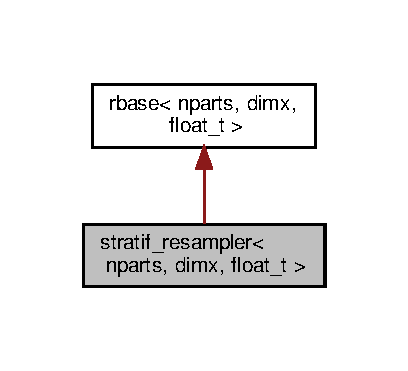
\includegraphics[width=196pt]{classstratif__resampler__inherit__graph}
\end{center}
\end{figure}


Collaboration diagram for stratif\+\_\+resampler$<$ nparts, dimx, float\+\_\+t $>$\+:\nopagebreak
\begin{figure}[H]
\begin{center}
\leavevmode
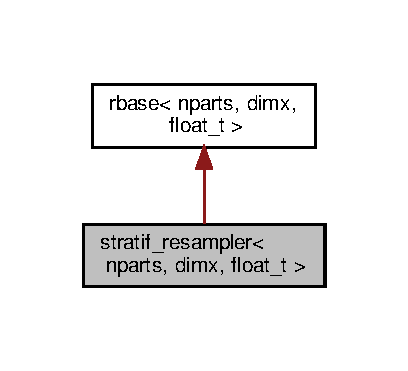
\includegraphics[width=196pt]{classstratif__resampler__coll__graph}
\end{center}
\end{figure}
\subsection*{Public Types}
\begin{DoxyCompactItemize}
\item 
using \hyperlink{classstratif__resampler_a9b8a1de85ef718528f4c889678a9331f}{ssv} = Eigen\+::\+Matrix$<$ float\+\_\+t, dimx, 1 $>$
\item 
using \hyperlink{classstratif__resampler_aafc4c3078fcc2912b41ad76465d86491}{array\+Vec} = std\+::array$<$ \hyperlink{classrbase_ae20e0b8df15aa109252f57ecbf1f20f8}{ssv}, nparts $>$
\item 
using \hyperlink{classstratif__resampler_ad85a57b7463ac619bb3123a2cd20bb01}{array\+Float} = std\+::array$<$ float\+\_\+t, nparts $>$
\item 
using \hyperlink{classstratif__resampler_a6feed5616bbd45f1bcf155fdf6348e19}{array\+Int} = std\+::array$<$ unsigned int, nparts $>$
\end{DoxyCompactItemize}
\subsection*{Public Member Functions}
\begin{DoxyCompactItemize}
\item 
\mbox{\Hypertarget{classstratif__resampler_a76e8fbfaec214060f0644d5a076c2b2a}\label{classstratif__resampler_a76e8fbfaec214060f0644d5a076c2b2a}} 
\hyperlink{classstratif__resampler_a76e8fbfaec214060f0644d5a076c2b2a}{stratif\+\_\+resampler} ()=default
\begin{DoxyCompactList}\small\item\em Default constructor. Only option available. \end{DoxyCompactList}\item 
void \hyperlink{classstratif__resampler_a2588147563bf3fe598e262cae7e125e6}{resamp\+Log\+Wts} (\hyperlink{classrbase_aa12fc826befa6ba0647b5f59ebc396ee}{array\+Vec} \&old\+Parts, \hyperlink{classrbase_a6f76bef853e508cb5b6f546d231b06f5}{array\+Float} \&old\+Log\+Un\+Norm\+Wts)
\begin{DoxyCompactList}\small\item\em resamples particles. \end{DoxyCompactList}\end{DoxyCompactItemize}
\subsection*{Additional Inherited Members}


\subsection{Detailed Description}
\subsubsection*{template$<$size\+\_\+t nparts, size\+\_\+t dimx, typename float\+\_\+t$>$\newline
class stratif\+\_\+resampler$<$ nparts, dimx, float\+\_\+t $>$}

\begin{DoxyAuthor}{Author}
taylor 
\end{DoxyAuthor}
\begin{DoxyDate}{Date}
10/25/19 
\end{DoxyDate}


\subsection{Member Typedef Documentation}
\mbox{\Hypertarget{classstratif__resampler_ad85a57b7463ac619bb3123a2cd20bb01}\label{classstratif__resampler_ad85a57b7463ac619bb3123a2cd20bb01}} 
\index{stratif\+\_\+resampler@{stratif\+\_\+resampler}!array\+Float@{array\+Float}}
\index{array\+Float@{array\+Float}!stratif\+\_\+resampler@{stratif\+\_\+resampler}}
\subsubsection{\texorpdfstring{array\+Float}{arrayFloat}}
{\footnotesize\ttfamily template$<$size\+\_\+t nparts, size\+\_\+t dimx, typename float\+\_\+t $>$ \\
using \hyperlink{classstratif__resampler}{stratif\+\_\+resampler}$<$ nparts, dimx, float\+\_\+t $>$\+::\hyperlink{classrbase_a6f76bef853e508cb5b6f546d231b06f5}{array\+Float} =  std\+::array$<$float\+\_\+t,nparts$>$}

type alias for array of float\+\_\+ts \mbox{\Hypertarget{classstratif__resampler_a6feed5616bbd45f1bcf155fdf6348e19}\label{classstratif__resampler_a6feed5616bbd45f1bcf155fdf6348e19}} 
\index{stratif\+\_\+resampler@{stratif\+\_\+resampler}!array\+Int@{array\+Int}}
\index{array\+Int@{array\+Int}!stratif\+\_\+resampler@{stratif\+\_\+resampler}}
\subsubsection{\texorpdfstring{array\+Int}{arrayInt}}
{\footnotesize\ttfamily template$<$size\+\_\+t nparts, size\+\_\+t dimx, typename float\+\_\+t $>$ \\
using \hyperlink{classstratif__resampler}{stratif\+\_\+resampler}$<$ nparts, dimx, float\+\_\+t $>$\+::\hyperlink{classstratif__resampler_a6feed5616bbd45f1bcf155fdf6348e19}{array\+Int} =  std\+::array$<$unsigned int, nparts$>$}

type alias for array of integers \mbox{\Hypertarget{classstratif__resampler_aafc4c3078fcc2912b41ad76465d86491}\label{classstratif__resampler_aafc4c3078fcc2912b41ad76465d86491}} 
\index{stratif\+\_\+resampler@{stratif\+\_\+resampler}!array\+Vec@{array\+Vec}}
\index{array\+Vec@{array\+Vec}!stratif\+\_\+resampler@{stratif\+\_\+resampler}}
\subsubsection{\texorpdfstring{array\+Vec}{arrayVec}}
{\footnotesize\ttfamily template$<$size\+\_\+t nparts, size\+\_\+t dimx, typename float\+\_\+t $>$ \\
using \hyperlink{classstratif__resampler}{stratif\+\_\+resampler}$<$ nparts, dimx, float\+\_\+t $>$\+::\hyperlink{classrbase_aa12fc826befa6ba0647b5f59ebc396ee}{array\+Vec} =  std\+::array$<$\hyperlink{classrbase_ae20e0b8df15aa109252f57ecbf1f20f8}{ssv}, nparts$>$}

type alias for array of Eigen Matrices \mbox{\Hypertarget{classstratif__resampler_a9b8a1de85ef718528f4c889678a9331f}\label{classstratif__resampler_a9b8a1de85ef718528f4c889678a9331f}} 
\index{stratif\+\_\+resampler@{stratif\+\_\+resampler}!ssv@{ssv}}
\index{ssv@{ssv}!stratif\+\_\+resampler@{stratif\+\_\+resampler}}
\subsubsection{\texorpdfstring{ssv}{ssv}}
{\footnotesize\ttfamily template$<$size\+\_\+t nparts, size\+\_\+t dimx, typename float\+\_\+t $>$ \\
using \hyperlink{classstratif__resampler}{stratif\+\_\+resampler}$<$ nparts, dimx, float\+\_\+t $>$\+::\hyperlink{classrbase_ae20e0b8df15aa109252f57ecbf1f20f8}{ssv} =  Eigen\+::\+Matrix$<$float\+\_\+t,dimx,1$>$}

type alias for linear algebra stuff 

\subsection{Member Function Documentation}
\mbox{\Hypertarget{classstratif__resampler_a2588147563bf3fe598e262cae7e125e6}\label{classstratif__resampler_a2588147563bf3fe598e262cae7e125e6}} 
\index{stratif\+\_\+resampler@{stratif\+\_\+resampler}!resamp\+Log\+Wts@{resamp\+Log\+Wts}}
\index{resamp\+Log\+Wts@{resamp\+Log\+Wts}!stratif\+\_\+resampler@{stratif\+\_\+resampler}}
\subsubsection{\texorpdfstring{resamp\+Log\+Wts()}{resampLogWts()}}
{\footnotesize\ttfamily template$<$size\+\_\+t nparts, size\+\_\+t dimx, typename float\+\_\+t $>$ \\
void \hyperlink{classstratif__resampler}{stratif\+\_\+resampler}$<$ nparts, dimx, float\+\_\+t $>$\+::resamp\+Log\+Wts (\begin{DoxyParamCaption}\item[{\hyperlink{classrbase_aa12fc826befa6ba0647b5f59ebc396ee}{array\+Vec} \&}]{old\+Parts,  }\item[{\hyperlink{classrbase_a6f76bef853e508cb5b6f546d231b06f5}{array\+Float} \&}]{old\+Log\+Un\+Norm\+Wts }\end{DoxyParamCaption})\hspace{0.3cm}{\ttfamily [virtual]}}



resamples particles. 


\begin{DoxyParams}{Parameters}
{\em old\+Parts} & the old particles \\
\hline
{\em old\+Log\+Un\+Norm\+Wts} & the old log unnormalized weights \\
\hline
\end{DoxyParams}


Implements \hyperlink{classrbase_aff0f6f88fd4656e67f5ebc870f10dd44}{rbase$<$ nparts, dimx, float\+\_\+t $>$}.



The documentation for this class was generated from the following file\+:\begin{DoxyCompactItemize}
\item 
include/pf/\hyperlink{resamplers_8h}{resamplers.\+h}\end{DoxyCompactItemize}

\hypertarget{classsystematic__resampler}{}\section{systematic\+\_\+resampler$<$ nparts, dimx, float\+\_\+t $>$ Class Template Reference}
\label{classsystematic__resampler}\index{systematic\+\_\+resampler$<$ nparts, dimx, float\+\_\+t $>$@{systematic\+\_\+resampler$<$ nparts, dimx, float\+\_\+t $>$}}


{\ttfamily \#include $<$resamplers.\+h$>$}



Inheritance diagram for systematic\+\_\+resampler$<$ nparts, dimx, float\+\_\+t $>$\+:
\nopagebreak
\begin{figure}[H]
\begin{center}
\leavevmode
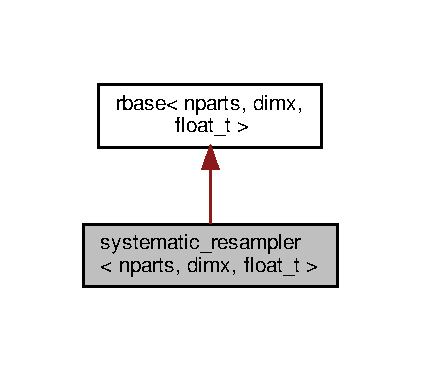
\includegraphics[width=202pt]{classsystematic__resampler__inherit__graph}
\end{center}
\end{figure}


Collaboration diagram for systematic\+\_\+resampler$<$ nparts, dimx, float\+\_\+t $>$\+:
\nopagebreak
\begin{figure}[H]
\begin{center}
\leavevmode
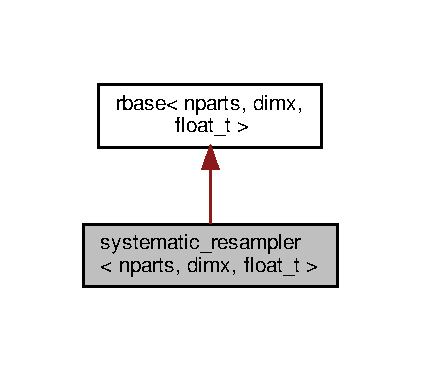
\includegraphics[width=202pt]{classsystematic__resampler__coll__graph}
\end{center}
\end{figure}
\subsection*{Public Types}
\begin{DoxyCompactItemize}
\item 
using \hyperlink{classsystematic__resampler_a9e158fbf5875f93e9cb4da562928e649}{ssv} = Eigen\+::\+Matrix$<$ float\+\_\+t, dimx, 1 $>$
\item 
using \hyperlink{classsystematic__resampler_a89263b385b61687341d67a717da78dc1}{array\+Vec} = std\+::array$<$ \hyperlink{classrbase_ae20e0b8df15aa109252f57ecbf1f20f8}{ssv}, nparts $>$
\item 
using \hyperlink{classsystematic__resampler_ae3f8e7d5687c068b7fc320fe4ee67871}{array\+Float} = std\+::array$<$ float\+\_\+t, nparts $>$
\item 
using \hyperlink{classsystematic__resampler_afbdf5779938dfee726f87d31040284de}{array\+Int} = std\+::array$<$ unsigned int, nparts $>$
\end{DoxyCompactItemize}
\subsection*{Public Member Functions}
\begin{DoxyCompactItemize}
\item 
\mbox{\Hypertarget{classsystematic__resampler_a6422f70f1f5315d16b018cb855435511}\label{classsystematic__resampler_a6422f70f1f5315d16b018cb855435511}} 
\hyperlink{classsystematic__resampler_a6422f70f1f5315d16b018cb855435511}{systematic\+\_\+resampler} ()=default
\begin{DoxyCompactList}\small\item\em Default constructor. Only option available. \end{DoxyCompactList}\item 
void \hyperlink{classsystematic__resampler_a9467aec6002043f35f40e9e4857021ed}{resamp\+Log\+Wts} (\hyperlink{classrbase_aa12fc826befa6ba0647b5f59ebc396ee}{array\+Vec} \&old\+Parts, \hyperlink{classrbase_a6f76bef853e508cb5b6f546d231b06f5}{array\+Float} \&old\+Log\+Un\+Norm\+Wts)
\begin{DoxyCompactList}\small\item\em resamples particles. \end{DoxyCompactList}\end{DoxyCompactItemize}
\subsection*{Additional Inherited Members}


\subsection{Detailed Description}
\subsubsection*{template$<$size\+\_\+t nparts, size\+\_\+t dimx, typename float\+\_\+t$>$\newline
class systematic\+\_\+resampler$<$ nparts, dimx, float\+\_\+t $>$}

\begin{DoxyAuthor}{Author}
taylor 
\end{DoxyAuthor}
\begin{DoxyDate}{Date}
10/25/19 
\end{DoxyDate}


\subsection{Member Typedef Documentation}
\mbox{\Hypertarget{classsystematic__resampler_ae3f8e7d5687c068b7fc320fe4ee67871}\label{classsystematic__resampler_ae3f8e7d5687c068b7fc320fe4ee67871}} 
\index{systematic\+\_\+resampler@{systematic\+\_\+resampler}!array\+Float@{array\+Float}}
\index{array\+Float@{array\+Float}!systematic\+\_\+resampler@{systematic\+\_\+resampler}}
\subsubsection{\texorpdfstring{array\+Float}{arrayFloat}}
{\footnotesize\ttfamily template$<$size\+\_\+t nparts, size\+\_\+t dimx, typename float\+\_\+t $>$ \\
using \hyperlink{classsystematic__resampler}{systematic\+\_\+resampler}$<$ nparts, dimx, float\+\_\+t $>$\+::\hyperlink{classrbase_a6f76bef853e508cb5b6f546d231b06f5}{array\+Float} =  std\+::array$<$float\+\_\+t,nparts$>$}

type alias for array of float\+\_\+ts \mbox{\Hypertarget{classsystematic__resampler_afbdf5779938dfee726f87d31040284de}\label{classsystematic__resampler_afbdf5779938dfee726f87d31040284de}} 
\index{systematic\+\_\+resampler@{systematic\+\_\+resampler}!array\+Int@{array\+Int}}
\index{array\+Int@{array\+Int}!systematic\+\_\+resampler@{systematic\+\_\+resampler}}
\subsubsection{\texorpdfstring{array\+Int}{arrayInt}}
{\footnotesize\ttfamily template$<$size\+\_\+t nparts, size\+\_\+t dimx, typename float\+\_\+t $>$ \\
using \hyperlink{classsystematic__resampler}{systematic\+\_\+resampler}$<$ nparts, dimx, float\+\_\+t $>$\+::\hyperlink{classsystematic__resampler_afbdf5779938dfee726f87d31040284de}{array\+Int} =  std\+::array$<$unsigned int, nparts$>$}

type alias for array of integers \mbox{\Hypertarget{classsystematic__resampler_a89263b385b61687341d67a717da78dc1}\label{classsystematic__resampler_a89263b385b61687341d67a717da78dc1}} 
\index{systematic\+\_\+resampler@{systematic\+\_\+resampler}!array\+Vec@{array\+Vec}}
\index{array\+Vec@{array\+Vec}!systematic\+\_\+resampler@{systematic\+\_\+resampler}}
\subsubsection{\texorpdfstring{array\+Vec}{arrayVec}}
{\footnotesize\ttfamily template$<$size\+\_\+t nparts, size\+\_\+t dimx, typename float\+\_\+t $>$ \\
using \hyperlink{classsystematic__resampler}{systematic\+\_\+resampler}$<$ nparts, dimx, float\+\_\+t $>$\+::\hyperlink{classrbase_aa12fc826befa6ba0647b5f59ebc396ee}{array\+Vec} =  std\+::array$<$\hyperlink{classrbase_ae20e0b8df15aa109252f57ecbf1f20f8}{ssv}, nparts$>$}

type alias for array of Eigen Matrices \mbox{\Hypertarget{classsystematic__resampler_a9e158fbf5875f93e9cb4da562928e649}\label{classsystematic__resampler_a9e158fbf5875f93e9cb4da562928e649}} 
\index{systematic\+\_\+resampler@{systematic\+\_\+resampler}!ssv@{ssv}}
\index{ssv@{ssv}!systematic\+\_\+resampler@{systematic\+\_\+resampler}}
\subsubsection{\texorpdfstring{ssv}{ssv}}
{\footnotesize\ttfamily template$<$size\+\_\+t nparts, size\+\_\+t dimx, typename float\+\_\+t $>$ \\
using \hyperlink{classsystematic__resampler}{systematic\+\_\+resampler}$<$ nparts, dimx, float\+\_\+t $>$\+::\hyperlink{classrbase_ae20e0b8df15aa109252f57ecbf1f20f8}{ssv} =  Eigen\+::\+Matrix$<$float\+\_\+t,dimx,1$>$}

type alias for linear algebra stuff 

\subsection{Member Function Documentation}
\mbox{\Hypertarget{classsystematic__resampler_a9467aec6002043f35f40e9e4857021ed}\label{classsystematic__resampler_a9467aec6002043f35f40e9e4857021ed}} 
\index{systematic\+\_\+resampler@{systematic\+\_\+resampler}!resamp\+Log\+Wts@{resamp\+Log\+Wts}}
\index{resamp\+Log\+Wts@{resamp\+Log\+Wts}!systematic\+\_\+resampler@{systematic\+\_\+resampler}}
\subsubsection{\texorpdfstring{resamp\+Log\+Wts()}{resampLogWts()}}
{\footnotesize\ttfamily template$<$size\+\_\+t nparts, size\+\_\+t dimx, typename float\+\_\+t $>$ \\
void \hyperlink{classsystematic__resampler}{systematic\+\_\+resampler}$<$ nparts, dimx, float\+\_\+t $>$\+::resamp\+Log\+Wts (\begin{DoxyParamCaption}\item[{\hyperlink{classrbase_aa12fc826befa6ba0647b5f59ebc396ee}{array\+Vec} \&}]{old\+Parts,  }\item[{\hyperlink{classrbase_a6f76bef853e508cb5b6f546d231b06f5}{array\+Float} \&}]{old\+Log\+Un\+Norm\+Wts }\end{DoxyParamCaption})\hspace{0.3cm}{\ttfamily [virtual]}}



resamples particles. 


\begin{DoxyParams}{Parameters}
{\em old\+Parts} & the old particles \\
\hline
{\em old\+Log\+Un\+Norm\+Wts} & the old log unnormalized weights \\
\hline
\end{DoxyParams}


Implements \hyperlink{classrbase_aff0f6f88fd4656e67f5ebc870f10dd44}{rbase$<$ nparts, dimx, float\+\_\+t $>$}.



The documentation for this class was generated from the following file\+:\begin{DoxyCompactItemize}
\item 
include/\hyperlink{resamplers_8h}{resamplers.\+h}\end{DoxyCompactItemize}

\hypertarget{classrvsamp_1_1TruncUnivNormSampler}{}\section{rvsamp\+:\+:Trunc\+Univ\+Norm\+Sampler$<$ float\+\_\+t $>$ Class Template Reference}
\label{classrvsamp_1_1TruncUnivNormSampler}\index{rvsamp\+::\+Trunc\+Univ\+Norm\+Sampler$<$ float\+\_\+t $>$@{rvsamp\+::\+Trunc\+Univ\+Norm\+Sampler$<$ float\+\_\+t $>$}}


Default-\/constructor ...  




{\ttfamily \#include $<$rv\+\_\+samp.\+h$>$}



Inheritance diagram for rvsamp\+:\+:Trunc\+Univ\+Norm\+Sampler$<$ float\+\_\+t $>$\+:\nopagebreak
\begin{figure}[H]
\begin{center}
\leavevmode
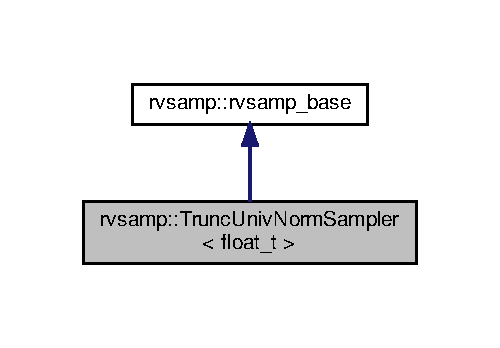
\includegraphics[width=240pt]{classrvsamp_1_1TruncUnivNormSampler__inherit__graph}
\end{center}
\end{figure}


Collaboration diagram for rvsamp\+:\+:Trunc\+Univ\+Norm\+Sampler$<$ float\+\_\+t $>$\+:\nopagebreak
\begin{figure}[H]
\begin{center}
\leavevmode
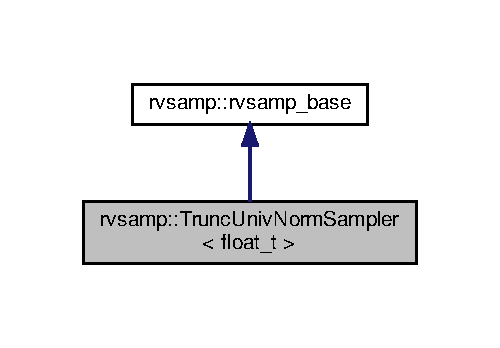
\includegraphics[width=240pt]{classrvsamp_1_1TruncUnivNormSampler__coll__graph}
\end{center}
\end{figure}
\subsection*{Public Member Functions}
\begin{DoxyCompactItemize}
\item 
\hyperlink{classrvsamp_1_1TruncUnivNormSampler_a937288fd46dcfef2f88de8081bb13752}{Trunc\+Univ\+Norm\+Sampler} (const float\+\_\+t \&mu, const float\+\_\+t \&sigma, const float\+\_\+t \&lower, const float\+\_\+t \&upper)
\begin{DoxyCompactList}\small\item\em The user must supply both mean and std. dev. \end{DoxyCompactList}\item 
float\+\_\+t \hyperlink{classrvsamp_1_1TruncUnivNormSampler_a2d6a8f2053e4ed0806718e6749288dce}{sample} ()
\begin{DoxyCompactList}\small\item\em Draws a random number. \end{DoxyCompactList}\end{DoxyCompactItemize}
\subsection*{Private Attributes}
\begin{DoxyCompactItemize}
\item 
\mbox{\Hypertarget{classrvsamp_1_1TruncUnivNormSampler_a272eeaa23053de1bad153f34a7c34329}\label{classrvsamp_1_1TruncUnivNormSampler_a272eeaa23053de1bad153f34a7c34329}} 
std\+::normal\+\_\+distribution$<$ float\+\_\+t $>$ \hyperlink{classrvsamp_1_1TruncUnivNormSampler_a272eeaa23053de1bad153f34a7c34329}{m\+\_\+z\+\_\+gen}
\begin{DoxyCompactList}\small\item\em makes normal random variates \end{DoxyCompactList}\item 
\mbox{\Hypertarget{classrvsamp_1_1TruncUnivNormSampler_a7c1024d6d70fec2999d611512f4c30b4}\label{classrvsamp_1_1TruncUnivNormSampler_a7c1024d6d70fec2999d611512f4c30b4}} 
float\+\_\+t \hyperlink{classrvsamp_1_1TruncUnivNormSampler_a7c1024d6d70fec2999d611512f4c30b4}{m\+\_\+mu}
\begin{DoxyCompactList}\small\item\em the mean \end{DoxyCompactList}\item 
\mbox{\Hypertarget{classrvsamp_1_1TruncUnivNormSampler_af54c9b539c82e865952e938cee75df1b}\label{classrvsamp_1_1TruncUnivNormSampler_af54c9b539c82e865952e938cee75df1b}} 
float\+\_\+t \hyperlink{classrvsamp_1_1TruncUnivNormSampler_af54c9b539c82e865952e938cee75df1b}{m\+\_\+sigma}
\begin{DoxyCompactList}\small\item\em the standard deviation \end{DoxyCompactList}\item 
\mbox{\Hypertarget{classrvsamp_1_1TruncUnivNormSampler_a6405f385e9fb923d5aeae60324b745c1}\label{classrvsamp_1_1TruncUnivNormSampler_a6405f385e9fb923d5aeae60324b745c1}} 
float\+\_\+t \hyperlink{classrvsamp_1_1TruncUnivNormSampler_a6405f385e9fb923d5aeae60324b745c1}{m\+\_\+lower}
\begin{DoxyCompactList}\small\item\em the lower bound \end{DoxyCompactList}\item 
\mbox{\Hypertarget{classrvsamp_1_1TruncUnivNormSampler_a5081f5dfd44015a5af38572a4a22bf58}\label{classrvsamp_1_1TruncUnivNormSampler_a5081f5dfd44015a5af38572a4a22bf58}} 
float\+\_\+t \hyperlink{classrvsamp_1_1TruncUnivNormSampler_a5081f5dfd44015a5af38572a4a22bf58}{m\+\_\+upper}
\begin{DoxyCompactList}\small\item\em the upper bound \end{DoxyCompactList}\end{DoxyCompactItemize}
\subsection*{Additional Inherited Members}


\subsection{Detailed Description}
\subsubsection*{template$<$typename float\+\_\+t$>$\newline
class rvsamp\+::\+Trunc\+Univ\+Norm\+Sampler$<$ float\+\_\+t $>$}

Default-\/constructor ... 

! A class that performs sampling from a univariate Gamma distribution. $\ast$$\ast$ The user must supply both mu and sigma. 
\begin{DoxyParams}{Parameters}
{\em mu} & a location parameter for the logarithm of the sample. \\
\hline
{\em sigma} & a positive scale parameter for the logarithm of the sample. sets the scale parameter of the logged random variable. \\
\hline
{\em sigma} & the desired parameter. sets the location parameter of the logged random variable. \\
\hline
{\em mu} & the desired parameter. draws a random number. \\
\hline
\end{DoxyParams}
\begin{DoxyReturn}{Returns}
a random sample of type float\+\_\+t.\+makes normal random variates mu sigma A class that performs sampling from a truncated univariate Normal distribution.
\end{DoxyReturn}
\begin{DoxyAuthor}{Author}
taylor 
\end{DoxyAuthor}


\subsection{Constructor \& Destructor Documentation}
\mbox{\Hypertarget{classrvsamp_1_1TruncUnivNormSampler_a937288fd46dcfef2f88de8081bb13752}\label{classrvsamp_1_1TruncUnivNormSampler_a937288fd46dcfef2f88de8081bb13752}} 
\index{rvsamp\+::\+Trunc\+Univ\+Norm\+Sampler@{rvsamp\+::\+Trunc\+Univ\+Norm\+Sampler}!Trunc\+Univ\+Norm\+Sampler@{Trunc\+Univ\+Norm\+Sampler}}
\index{Trunc\+Univ\+Norm\+Sampler@{Trunc\+Univ\+Norm\+Sampler}!rvsamp\+::\+Trunc\+Univ\+Norm\+Sampler@{rvsamp\+::\+Trunc\+Univ\+Norm\+Sampler}}
\subsubsection{\texorpdfstring{Trunc\+Univ\+Norm\+Sampler()}{TruncUnivNormSampler()}}
{\footnotesize\ttfamily template$<$typename float\+\_\+t $>$ \\
\hyperlink{classrvsamp_1_1TruncUnivNormSampler}{rvsamp\+::\+Trunc\+Univ\+Norm\+Sampler}$<$ float\+\_\+t $>$\+::\hyperlink{classrvsamp_1_1TruncUnivNormSampler}{Trunc\+Univ\+Norm\+Sampler} (\begin{DoxyParamCaption}\item[{const float\+\_\+t \&}]{mu,  }\item[{const float\+\_\+t \&}]{sigma,  }\item[{const float\+\_\+t \&}]{lower,  }\item[{const float\+\_\+t \&}]{upper }\end{DoxyParamCaption})}



The user must supply both mean and std. dev. 


\begin{DoxyParams}{Parameters}
{\em mu} & a float\+\_\+t for the location parameter. \\
\hline
{\em sigma} & a float\+\_\+t ($>$ 0) representing the scale of the samples. \\
\hline
{\em lower} & the lower bound of the support \\
\hline
{\em upper} & the upper bound of the support \\
\hline
\end{DoxyParams}


\subsection{Member Function Documentation}
\mbox{\Hypertarget{classrvsamp_1_1TruncUnivNormSampler_a2d6a8f2053e4ed0806718e6749288dce}\label{classrvsamp_1_1TruncUnivNormSampler_a2d6a8f2053e4ed0806718e6749288dce}} 
\index{rvsamp\+::\+Trunc\+Univ\+Norm\+Sampler@{rvsamp\+::\+Trunc\+Univ\+Norm\+Sampler}!sample@{sample}}
\index{sample@{sample}!rvsamp\+::\+Trunc\+Univ\+Norm\+Sampler@{rvsamp\+::\+Trunc\+Univ\+Norm\+Sampler}}
\subsubsection{\texorpdfstring{sample()}{sample()}}
{\footnotesize\ttfamily template$<$typename float\+\_\+t $>$ \\
float\+\_\+t \hyperlink{classrvsamp_1_1TruncUnivNormSampler}{rvsamp\+::\+Trunc\+Univ\+Norm\+Sampler}$<$ float\+\_\+t $>$\+::sample (\begin{DoxyParamCaption}{ }\end{DoxyParamCaption})}



Draws a random number. 

\begin{DoxyReturn}{Returns}
a random sample of type float\+\_\+t. 
\end{DoxyReturn}


The documentation for this class was generated from the following file\+:\begin{DoxyCompactItemize}
\item 
include/\hyperlink{rv__samp_8h}{rv\+\_\+samp.\+h}\end{DoxyCompactItemize}

\hypertarget{classrvsamp_1_1UniformSampler}{}\section{rvsamp\+:\+:Uniform\+Sampler$<$ float\+\_\+t $>$ Class Template Reference}
\label{classrvsamp_1_1UniformSampler}\index{rvsamp\+::\+Uniform\+Sampler$<$ float\+\_\+t $>$@{rvsamp\+::\+Uniform\+Sampler$<$ float\+\_\+t $>$}}


A class that performs sampling from a continuous uniform distribution.  




{\ttfamily \#include $<$rv\+\_\+samp.\+h$>$}



Inheritance diagram for rvsamp\+:\+:Uniform\+Sampler$<$ float\+\_\+t $>$\+:\nopagebreak
\begin{figure}[H]
\begin{center}
\leavevmode
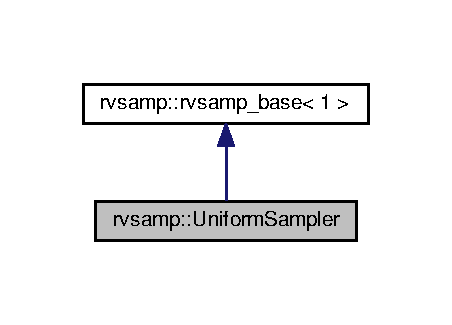
\includegraphics[width=205pt]{classrvsamp_1_1UniformSampler__inherit__graph}
\end{center}
\end{figure}


Collaboration diagram for rvsamp\+:\+:Uniform\+Sampler$<$ float\+\_\+t $>$\+:\nopagebreak
\begin{figure}[H]
\begin{center}
\leavevmode
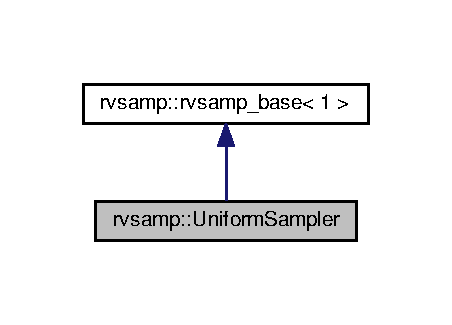
\includegraphics[width=205pt]{classrvsamp_1_1UniformSampler__coll__graph}
\end{center}
\end{figure}
\subsection*{Public Member Functions}
\begin{DoxyCompactItemize}
\item 
\mbox{\Hypertarget{classrvsamp_1_1UniformSampler_a0e1d5480bdc2a16d8d4ff39710c06e22}\label{classrvsamp_1_1UniformSampler_a0e1d5480bdc2a16d8d4ff39710c06e22}} 
\hyperlink{classrvsamp_1_1UniformSampler_a0e1d5480bdc2a16d8d4ff39710c06e22}{Uniform\+Sampler} ()
\begin{DoxyCompactList}\small\item\em The default constructor. Gives a lower bound of 0 and upper bound of 1. \end{DoxyCompactList}\item 
\hyperlink{classrvsamp_1_1UniformSampler_a909a8202baf85b8b541d6e339c0e1b18}{Uniform\+Sampler} (float\+\_\+t lower, float\+\_\+t upper)
\begin{DoxyCompactList}\small\item\em The constructor. \end{DoxyCompactList}\item 
float\+\_\+t \hyperlink{classrvsamp_1_1UniformSampler_acc8866283171489eccc5f643269b6eed}{sample} ()
\begin{DoxyCompactList}\small\item\em Draws a sample. \end{DoxyCompactList}\end{DoxyCompactItemize}
\subsection*{Private Attributes}
\begin{DoxyCompactItemize}
\item 
\mbox{\Hypertarget{classrvsamp_1_1UniformSampler_a015cefddd5e6e88f8a7318daec2211cc}\label{classrvsamp_1_1UniformSampler_a015cefddd5e6e88f8a7318daec2211cc}} 
std\+::uniform\+\_\+real\+\_\+distribution$<$ float\+\_\+t $>$ \hyperlink{classrvsamp_1_1UniformSampler_a015cefddd5e6e88f8a7318daec2211cc}{m\+\_\+unif\+\_\+gen}
\begin{DoxyCompactList}\small\item\em makes uniform random variates \end{DoxyCompactList}\end{DoxyCompactItemize}
\subsection*{Additional Inherited Members}


\subsection{Detailed Description}
\subsubsection*{template$<$typename float\+\_\+t$>$\newline
class rvsamp\+::\+Uniform\+Sampler$<$ float\+\_\+t $>$}

A class that performs sampling from a continuous uniform distribution. 

\begin{DoxyAuthor}{Author}
taylor 
\end{DoxyAuthor}


\subsection{Constructor \& Destructor Documentation}
\mbox{\Hypertarget{classrvsamp_1_1UniformSampler_a909a8202baf85b8b541d6e339c0e1b18}\label{classrvsamp_1_1UniformSampler_a909a8202baf85b8b541d6e339c0e1b18}} 
\index{rvsamp\+::\+Uniform\+Sampler@{rvsamp\+::\+Uniform\+Sampler}!Uniform\+Sampler@{Uniform\+Sampler}}
\index{Uniform\+Sampler@{Uniform\+Sampler}!rvsamp\+::\+Uniform\+Sampler@{rvsamp\+::\+Uniform\+Sampler}}
\subsubsection{\texorpdfstring{Uniform\+Sampler()}{UniformSampler()}}
{\footnotesize\ttfamily template$<$typename float\+\_\+t $>$ \\
\hyperlink{classrvsamp_1_1UniformSampler}{rvsamp\+::\+Uniform\+Sampler}$<$ float\+\_\+t $>$\+::\hyperlink{classrvsamp_1_1UniformSampler}{Uniform\+Sampler} (\begin{DoxyParamCaption}\item[{float\+\_\+t}]{lower,  }\item[{float\+\_\+t}]{upper }\end{DoxyParamCaption})}



The constructor. 


\begin{DoxyParams}{Parameters}
{\em lower} & the lower bound of the P\+R\+NG. \\
\hline
{\em upper} & the upper bound of the P\+R\+NG. \\
\hline
\end{DoxyParams}


\subsection{Member Function Documentation}
\mbox{\Hypertarget{classrvsamp_1_1UniformSampler_acc8866283171489eccc5f643269b6eed}\label{classrvsamp_1_1UniformSampler_acc8866283171489eccc5f643269b6eed}} 
\index{rvsamp\+::\+Uniform\+Sampler@{rvsamp\+::\+Uniform\+Sampler}!sample@{sample}}
\index{sample@{sample}!rvsamp\+::\+Uniform\+Sampler@{rvsamp\+::\+Uniform\+Sampler}}
\subsubsection{\texorpdfstring{sample()}{sample()}}
{\footnotesize\ttfamily template$<$typename float\+\_\+t $>$ \\
float\+\_\+t \hyperlink{classrvsamp_1_1UniformSampler}{rvsamp\+::\+Uniform\+Sampler}$<$ float\+\_\+t $>$\+::sample (\begin{DoxyParamCaption}{ }\end{DoxyParamCaption})}



Draws a sample. 

\begin{DoxyReturn}{Returns}
a sample of type float\+\_\+t. 
\end{DoxyReturn}


The documentation for this class was generated from the following file\+:\begin{DoxyCompactItemize}
\item 
include/pf/\hyperlink{rv__samp_8h}{rv\+\_\+samp.\+h}\end{DoxyCompactItemize}

\hypertarget{classrvsamp_1_1UnivLogNormSampler}{}\section{rvsamp\+:\+:Univ\+Log\+Norm\+Sampler$<$ float\+\_\+t $>$ Class Template Reference}
\label{classrvsamp_1_1UnivLogNormSampler}\index{rvsamp\+::\+Univ\+Log\+Norm\+Sampler$<$ float\+\_\+t $>$@{rvsamp\+::\+Univ\+Log\+Norm\+Sampler$<$ float\+\_\+t $>$}}


A class that performs sampling from a univariate Log-\/\+Normal distribution.  




{\ttfamily \#include $<$rv\+\_\+samp.\+h$>$}



Inheritance diagram for rvsamp\+:\+:Univ\+Log\+Norm\+Sampler$<$ float\+\_\+t $>$\+:
\nopagebreak
\begin{figure}[H]
\begin{center}
\leavevmode
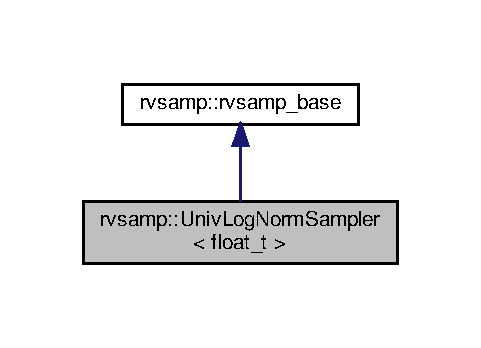
\includegraphics[width=231pt]{classrvsamp_1_1UnivLogNormSampler__inherit__graph}
\end{center}
\end{figure}


Collaboration diagram for rvsamp\+:\+:Univ\+Log\+Norm\+Sampler$<$ float\+\_\+t $>$\+:
\nopagebreak
\begin{figure}[H]
\begin{center}
\leavevmode
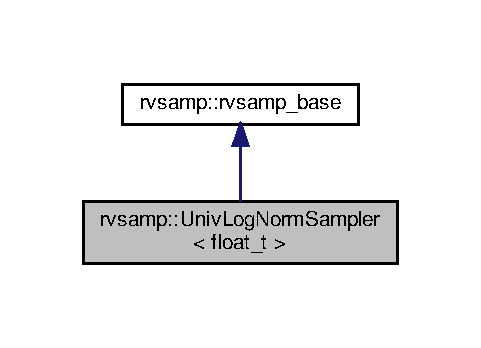
\includegraphics[width=231pt]{classrvsamp_1_1UnivLogNormSampler__coll__graph}
\end{center}
\end{figure}
\subsection*{Public Member Functions}
\begin{DoxyCompactItemize}
\item 
\mbox{\Hypertarget{classrvsamp_1_1UnivLogNormSampler_aa31a7d6a486257b4a8404b74c7887b11}\label{classrvsamp_1_1UnivLogNormSampler_aa31a7d6a486257b4a8404b74c7887b11}} 
\hyperlink{classrvsamp_1_1UnivLogNormSampler_aa31a7d6a486257b4a8404b74c7887b11}{Univ\+Log\+Norm\+Sampler} ()
\begin{DoxyCompactList}\small\item\em Default-\/constructor sets up for standard Normal random variate generation. \end{DoxyCompactList}\item 
\hyperlink{classrvsamp_1_1UnivLogNormSampler_a679213457584e98a7dc205a9b7d6a0cd}{Univ\+Log\+Norm\+Sampler} (const float\+\_\+t \&mu, const float\+\_\+t \&sigma)
\begin{DoxyCompactList}\small\item\em The user must supply both mu and sigma. \end{DoxyCompactList}\item 
void \hyperlink{classrvsamp_1_1UnivLogNormSampler_a21bdbf5f20b327f5905605dd0357c8b8}{set\+Sigma} (const float\+\_\+t \&sigma)
\begin{DoxyCompactList}\small\item\em sets the scale parameter of the logged random variable. \end{DoxyCompactList}\item 
void \hyperlink{classrvsamp_1_1UnivLogNormSampler_a43c00fb2c560c1444ccdee13060c5153}{set\+Mu} (const float\+\_\+t \&mu)
\begin{DoxyCompactList}\small\item\em sets the location parameter of the logged random variable. \end{DoxyCompactList}\item 
float\+\_\+t \hyperlink{classrvsamp_1_1UnivLogNormSampler_a816c87875ed08b4b90f9fbe3fd4bda88}{sample} ()
\begin{DoxyCompactList}\small\item\em draws a random number. \end{DoxyCompactList}\end{DoxyCompactItemize}
\subsection*{Private Attributes}
\begin{DoxyCompactItemize}
\item 
\mbox{\Hypertarget{classrvsamp_1_1UnivLogNormSampler_a2f41b8dd97ef6f0cd5537a2b11242cb6}\label{classrvsamp_1_1UnivLogNormSampler_a2f41b8dd97ef6f0cd5537a2b11242cb6}} 
std\+::normal\+\_\+distribution$<$ float\+\_\+t $>$ \hyperlink{classrvsamp_1_1UnivLogNormSampler_a2f41b8dd97ef6f0cd5537a2b11242cb6}{m\+\_\+z\+\_\+gen}
\begin{DoxyCompactList}\small\item\em makes normal random variates \end{DoxyCompactList}\item 
\mbox{\Hypertarget{classrvsamp_1_1UnivLogNormSampler_a94599a9ec4d17a1c68f77b5a6cb22a8d}\label{classrvsamp_1_1UnivLogNormSampler_a94599a9ec4d17a1c68f77b5a6cb22a8d}} 
float\+\_\+t \hyperlink{classrvsamp_1_1UnivLogNormSampler_a94599a9ec4d17a1c68f77b5a6cb22a8d}{m\+\_\+mu}
\begin{DoxyCompactList}\small\item\em mu \end{DoxyCompactList}\item 
\mbox{\Hypertarget{classrvsamp_1_1UnivLogNormSampler_a608a40aa21935aaa36a9c44f1a3392a4}\label{classrvsamp_1_1UnivLogNormSampler_a608a40aa21935aaa36a9c44f1a3392a4}} 
float\+\_\+t \hyperlink{classrvsamp_1_1UnivLogNormSampler_a608a40aa21935aaa36a9c44f1a3392a4}{m\+\_\+sigma}
\begin{DoxyCompactList}\small\item\em sigma \end{DoxyCompactList}\end{DoxyCompactItemize}
\subsection*{Additional Inherited Members}


\subsection{Detailed Description}
\subsubsection*{template$<$typename float\+\_\+t$>$\newline
class rvsamp\+::\+Univ\+Log\+Norm\+Sampler$<$ float\+\_\+t $>$}

A class that performs sampling from a univariate Log-\/\+Normal distribution. 

\begin{DoxyAuthor}{Author}
taylor 
\end{DoxyAuthor}


\subsection{Constructor \& Destructor Documentation}
\mbox{\Hypertarget{classrvsamp_1_1UnivLogNormSampler_a679213457584e98a7dc205a9b7d6a0cd}\label{classrvsamp_1_1UnivLogNormSampler_a679213457584e98a7dc205a9b7d6a0cd}} 
\index{rvsamp\+::\+Univ\+Log\+Norm\+Sampler@{rvsamp\+::\+Univ\+Log\+Norm\+Sampler}!Univ\+Log\+Norm\+Sampler@{Univ\+Log\+Norm\+Sampler}}
\index{Univ\+Log\+Norm\+Sampler@{Univ\+Log\+Norm\+Sampler}!rvsamp\+::\+Univ\+Log\+Norm\+Sampler@{rvsamp\+::\+Univ\+Log\+Norm\+Sampler}}
\subsubsection{\texorpdfstring{Univ\+Log\+Norm\+Sampler()}{UnivLogNormSampler()}}
{\footnotesize\ttfamily template$<$typename float\+\_\+t $>$ \\
\hyperlink{classrvsamp_1_1UnivLogNormSampler}{rvsamp\+::\+Univ\+Log\+Norm\+Sampler}$<$ float\+\_\+t $>$\+::\hyperlink{classrvsamp_1_1UnivLogNormSampler}{Univ\+Log\+Norm\+Sampler} (\begin{DoxyParamCaption}\item[{const float\+\_\+t \&}]{mu,  }\item[{const float\+\_\+t \&}]{sigma }\end{DoxyParamCaption})}



The user must supply both mu and sigma. 


\begin{DoxyParams}{Parameters}
{\em mu} & a location parameter for the logarithm of the sample. \\
\hline
{\em sigma} & a positive scale parameter for the logarithm of the sample. \\
\hline
\end{DoxyParams}


\subsection{Member Function Documentation}
\mbox{\Hypertarget{classrvsamp_1_1UnivLogNormSampler_a816c87875ed08b4b90f9fbe3fd4bda88}\label{classrvsamp_1_1UnivLogNormSampler_a816c87875ed08b4b90f9fbe3fd4bda88}} 
\index{rvsamp\+::\+Univ\+Log\+Norm\+Sampler@{rvsamp\+::\+Univ\+Log\+Norm\+Sampler}!sample@{sample}}
\index{sample@{sample}!rvsamp\+::\+Univ\+Log\+Norm\+Sampler@{rvsamp\+::\+Univ\+Log\+Norm\+Sampler}}
\subsubsection{\texorpdfstring{sample()}{sample()}}
{\footnotesize\ttfamily template$<$typename float\+\_\+t $>$ \\
float\+\_\+t \hyperlink{classrvsamp_1_1UnivLogNormSampler}{rvsamp\+::\+Univ\+Log\+Norm\+Sampler}$<$ float\+\_\+t $>$\+::sample (\begin{DoxyParamCaption}{ }\end{DoxyParamCaption})}



draws a random number. 

\begin{DoxyReturn}{Returns}
a random sample of type float\+\_\+t. 
\end{DoxyReturn}
\mbox{\Hypertarget{classrvsamp_1_1UnivLogNormSampler_a43c00fb2c560c1444ccdee13060c5153}\label{classrvsamp_1_1UnivLogNormSampler_a43c00fb2c560c1444ccdee13060c5153}} 
\index{rvsamp\+::\+Univ\+Log\+Norm\+Sampler@{rvsamp\+::\+Univ\+Log\+Norm\+Sampler}!set\+Mu@{set\+Mu}}
\index{set\+Mu@{set\+Mu}!rvsamp\+::\+Univ\+Log\+Norm\+Sampler@{rvsamp\+::\+Univ\+Log\+Norm\+Sampler}}
\subsubsection{\texorpdfstring{set\+Mu()}{setMu()}}
{\footnotesize\ttfamily template$<$typename float\+\_\+t $>$ \\
void \hyperlink{classrvsamp_1_1UnivLogNormSampler}{rvsamp\+::\+Univ\+Log\+Norm\+Sampler}$<$ float\+\_\+t $>$\+::set\+Mu (\begin{DoxyParamCaption}\item[{const float\+\_\+t \&}]{mu }\end{DoxyParamCaption})}



sets the location parameter of the logged random variable. 


\begin{DoxyParams}{Parameters}
{\em mu} & the desired parameter. \\
\hline
\end{DoxyParams}
\mbox{\Hypertarget{classrvsamp_1_1UnivLogNormSampler_a21bdbf5f20b327f5905605dd0357c8b8}\label{classrvsamp_1_1UnivLogNormSampler_a21bdbf5f20b327f5905605dd0357c8b8}} 
\index{rvsamp\+::\+Univ\+Log\+Norm\+Sampler@{rvsamp\+::\+Univ\+Log\+Norm\+Sampler}!set\+Sigma@{set\+Sigma}}
\index{set\+Sigma@{set\+Sigma}!rvsamp\+::\+Univ\+Log\+Norm\+Sampler@{rvsamp\+::\+Univ\+Log\+Norm\+Sampler}}
\subsubsection{\texorpdfstring{set\+Sigma()}{setSigma()}}
{\footnotesize\ttfamily template$<$typename float\+\_\+t $>$ \\
void \hyperlink{classrvsamp_1_1UnivLogNormSampler}{rvsamp\+::\+Univ\+Log\+Norm\+Sampler}$<$ float\+\_\+t $>$\+::set\+Sigma (\begin{DoxyParamCaption}\item[{const float\+\_\+t \&}]{sigma }\end{DoxyParamCaption})}



sets the scale parameter of the logged random variable. 


\begin{DoxyParams}{Parameters}
{\em sigma} & the desired parameter. \\
\hline
\end{DoxyParams}


The documentation for this class was generated from the following file\+:\begin{DoxyCompactItemize}
\item 
include/\hyperlink{rv__samp_8h}{rv\+\_\+samp.\+h}\end{DoxyCompactItemize}

\hypertarget{classrvsamp_1_1UnivNormSampler}{}\section{rvsamp\+:\+:Univ\+Norm\+Sampler$<$ float\+\_\+t $>$ Class Template Reference}
\label{classrvsamp_1_1UnivNormSampler}\index{rvsamp\+::\+Univ\+Norm\+Sampler$<$ float\+\_\+t $>$@{rvsamp\+::\+Univ\+Norm\+Sampler$<$ float\+\_\+t $>$}}


A class that performs sampling from a univariate Normal distribution.  




{\ttfamily \#include $<$rv\+\_\+samp.\+h$>$}



Inheritance diagram for rvsamp\+:\+:Univ\+Norm\+Sampler$<$ float\+\_\+t $>$\+:\nopagebreak
\begin{figure}[H]
\begin{center}
\leavevmode
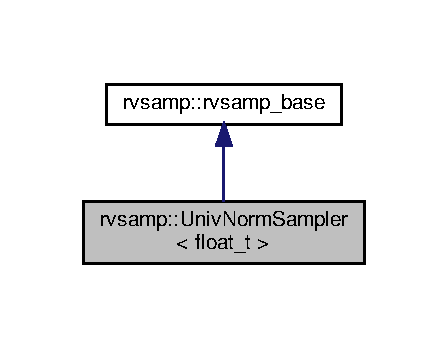
\includegraphics[width=215pt]{classrvsamp_1_1UnivNormSampler__inherit__graph}
\end{center}
\end{figure}


Collaboration diagram for rvsamp\+:\+:Univ\+Norm\+Sampler$<$ float\+\_\+t $>$\+:\nopagebreak
\begin{figure}[H]
\begin{center}
\leavevmode
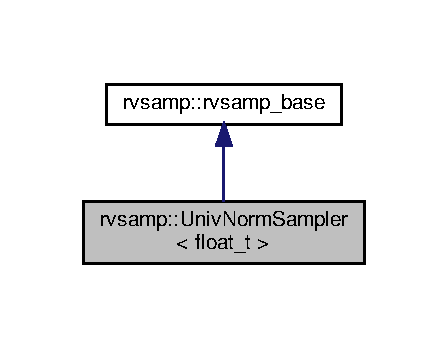
\includegraphics[width=215pt]{classrvsamp_1_1UnivNormSampler__coll__graph}
\end{center}
\end{figure}
\subsection*{Public Member Functions}
\begin{DoxyCompactItemize}
\item 
\mbox{\Hypertarget{classrvsamp_1_1UnivNormSampler_ade55cded90f94c26d4dfc309cf894a37}\label{classrvsamp_1_1UnivNormSampler_ade55cded90f94c26d4dfc309cf894a37}} 
\hyperlink{classrvsamp_1_1UnivNormSampler_ade55cded90f94c26d4dfc309cf894a37}{Univ\+Norm\+Sampler} ()
\begin{DoxyCompactList}\small\item\em Default-\/constructor sets up for standard Normal random variate generation. \end{DoxyCompactList}\item 
\hyperlink{classrvsamp_1_1UnivNormSampler_a9a643fec11776028014be75163819807}{Univ\+Norm\+Sampler} (float\+\_\+t mu, float\+\_\+t sigma)
\begin{DoxyCompactList}\small\item\em The user must supply both mean and std. dev. \end{DoxyCompactList}\item 
void \hyperlink{classrvsamp_1_1UnivNormSampler_a251f76fd8e9aa078d16bc01e53406681}{set\+Std\+Dev} (float\+\_\+t sigma)
\begin{DoxyCompactList}\small\item\em sets the standard deviation of the sampler. \end{DoxyCompactList}\item 
void \hyperlink{classrvsamp_1_1UnivNormSampler_a3969ca7da7cbea29ba766b3a87713049}{set\+Mean} (float\+\_\+t mu)
\begin{DoxyCompactList}\small\item\em sets the mean of the sampler. \end{DoxyCompactList}\item 
float\+\_\+t \hyperlink{classrvsamp_1_1UnivNormSampler_a67416efdbb1569a068d5a5a4914e27a1}{sample} ()
\begin{DoxyCompactList}\small\item\em Draws a random number. \end{DoxyCompactList}\end{DoxyCompactItemize}
\subsection*{Private Attributes}
\begin{DoxyCompactItemize}
\item 
\mbox{\Hypertarget{classrvsamp_1_1UnivNormSampler_a5c40c8154c9585acb70c9a487764806e}\label{classrvsamp_1_1UnivNormSampler_a5c40c8154c9585acb70c9a487764806e}} 
std\+::normal\+\_\+distribution$<$ float\+\_\+t $>$ \hyperlink{classrvsamp_1_1UnivNormSampler_a5c40c8154c9585acb70c9a487764806e}{m\+\_\+z\+\_\+gen}
\begin{DoxyCompactList}\small\item\em makes normal random variates \end{DoxyCompactList}\item 
\mbox{\Hypertarget{classrvsamp_1_1UnivNormSampler_a62483bf974fc36d79ff38aa81755e645}\label{classrvsamp_1_1UnivNormSampler_a62483bf974fc36d79ff38aa81755e645}} 
float\+\_\+t \hyperlink{classrvsamp_1_1UnivNormSampler_a62483bf974fc36d79ff38aa81755e645}{m\+\_\+mu}
\begin{DoxyCompactList}\small\item\em the mean \end{DoxyCompactList}\item 
\mbox{\Hypertarget{classrvsamp_1_1UnivNormSampler_a5ecc2ae8d9b2c25f070467651cf4f0d2}\label{classrvsamp_1_1UnivNormSampler_a5ecc2ae8d9b2c25f070467651cf4f0d2}} 
float\+\_\+t \hyperlink{classrvsamp_1_1UnivNormSampler_a5ecc2ae8d9b2c25f070467651cf4f0d2}{m\+\_\+sigma}
\begin{DoxyCompactList}\small\item\em the standard deviation \end{DoxyCompactList}\end{DoxyCompactItemize}
\subsection*{Additional Inherited Members}


\subsection{Detailed Description}
\subsubsection*{template$<$typename float\+\_\+t$>$\newline
class rvsamp\+::\+Univ\+Norm\+Sampler$<$ float\+\_\+t $>$}

A class that performs sampling from a univariate Normal distribution. 

\begin{DoxyAuthor}{Author}
taylor 
\end{DoxyAuthor}


\subsection{Constructor \& Destructor Documentation}
\mbox{\Hypertarget{classrvsamp_1_1UnivNormSampler_a9a643fec11776028014be75163819807}\label{classrvsamp_1_1UnivNormSampler_a9a643fec11776028014be75163819807}} 
\index{rvsamp\+::\+Univ\+Norm\+Sampler@{rvsamp\+::\+Univ\+Norm\+Sampler}!Univ\+Norm\+Sampler@{Univ\+Norm\+Sampler}}
\index{Univ\+Norm\+Sampler@{Univ\+Norm\+Sampler}!rvsamp\+::\+Univ\+Norm\+Sampler@{rvsamp\+::\+Univ\+Norm\+Sampler}}
\subsubsection{\texorpdfstring{Univ\+Norm\+Sampler()}{UnivNormSampler()}}
{\footnotesize\ttfamily template$<$typename float\+\_\+t $>$ \\
\hyperlink{classrvsamp_1_1UnivNormSampler}{rvsamp\+::\+Univ\+Norm\+Sampler}$<$ float\+\_\+t $>$\+::\hyperlink{classrvsamp_1_1UnivNormSampler}{Univ\+Norm\+Sampler} (\begin{DoxyParamCaption}\item[{float\+\_\+t}]{mu,  }\item[{float\+\_\+t}]{sigma }\end{DoxyParamCaption})}



The user must supply both mean and std. dev. 


\begin{DoxyParams}{Parameters}
{\em mu} & a float\+\_\+t for the mean of the sampling distribution. \\
\hline
{\em sigma} & a float\+\_\+t ($>$ 0) representing the standard deviation of the samples. \\
\hline
\end{DoxyParams}


\subsection{Member Function Documentation}
\mbox{\Hypertarget{classrvsamp_1_1UnivNormSampler_a67416efdbb1569a068d5a5a4914e27a1}\label{classrvsamp_1_1UnivNormSampler_a67416efdbb1569a068d5a5a4914e27a1}} 
\index{rvsamp\+::\+Univ\+Norm\+Sampler@{rvsamp\+::\+Univ\+Norm\+Sampler}!sample@{sample}}
\index{sample@{sample}!rvsamp\+::\+Univ\+Norm\+Sampler@{rvsamp\+::\+Univ\+Norm\+Sampler}}
\subsubsection{\texorpdfstring{sample()}{sample()}}
{\footnotesize\ttfamily template$<$typename float\+\_\+t $>$ \\
float\+\_\+t \hyperlink{classrvsamp_1_1UnivNormSampler}{rvsamp\+::\+Univ\+Norm\+Sampler}$<$ float\+\_\+t $>$\+::sample (\begin{DoxyParamCaption}{ }\end{DoxyParamCaption})}



Draws a random number. 

\begin{DoxyReturn}{Returns}
a random sample of type float\+\_\+t. 
\end{DoxyReturn}
\mbox{\Hypertarget{classrvsamp_1_1UnivNormSampler_a3969ca7da7cbea29ba766b3a87713049}\label{classrvsamp_1_1UnivNormSampler_a3969ca7da7cbea29ba766b3a87713049}} 
\index{rvsamp\+::\+Univ\+Norm\+Sampler@{rvsamp\+::\+Univ\+Norm\+Sampler}!set\+Mean@{set\+Mean}}
\index{set\+Mean@{set\+Mean}!rvsamp\+::\+Univ\+Norm\+Sampler@{rvsamp\+::\+Univ\+Norm\+Sampler}}
\subsubsection{\texorpdfstring{set\+Mean()}{setMean()}}
{\footnotesize\ttfamily template$<$typename float\+\_\+t $>$ \\
void \hyperlink{classrvsamp_1_1UnivNormSampler}{rvsamp\+::\+Univ\+Norm\+Sampler}$<$ float\+\_\+t $>$\+::set\+Mean (\begin{DoxyParamCaption}\item[{float\+\_\+t}]{mu }\end{DoxyParamCaption})}



sets the mean of the sampler. 


\begin{DoxyParams}{Parameters}
{\em mu} & the desired mean. \\
\hline
\end{DoxyParams}
\mbox{\Hypertarget{classrvsamp_1_1UnivNormSampler_a251f76fd8e9aa078d16bc01e53406681}\label{classrvsamp_1_1UnivNormSampler_a251f76fd8e9aa078d16bc01e53406681}} 
\index{rvsamp\+::\+Univ\+Norm\+Sampler@{rvsamp\+::\+Univ\+Norm\+Sampler}!set\+Std\+Dev@{set\+Std\+Dev}}
\index{set\+Std\+Dev@{set\+Std\+Dev}!rvsamp\+::\+Univ\+Norm\+Sampler@{rvsamp\+::\+Univ\+Norm\+Sampler}}
\subsubsection{\texorpdfstring{set\+Std\+Dev()}{setStdDev()}}
{\footnotesize\ttfamily template$<$typename float\+\_\+t $>$ \\
void \hyperlink{classrvsamp_1_1UnivNormSampler}{rvsamp\+::\+Univ\+Norm\+Sampler}$<$ float\+\_\+t $>$\+::set\+Std\+Dev (\begin{DoxyParamCaption}\item[{float\+\_\+t}]{sigma }\end{DoxyParamCaption})}



sets the standard deviation of the sampler. 


\begin{DoxyParams}{Parameters}
{\em sigma} & the desired standard deviation. \\
\hline
\end{DoxyParams}


The documentation for this class was generated from the following file\+:\begin{DoxyCompactItemize}
\item 
include/pf/\hyperlink{rv__samp_8h}{rv\+\_\+samp.\+h}\end{DoxyCompactItemize}

\chapter{File Documentation}
\hypertarget{auxiliary__pf_8h}{}\section{include/auxiliary\+\_\+pf.h File Reference}
\label{auxiliary__pf_8h}\index{include/auxiliary\+\_\+pf.\+h@{include/auxiliary\+\_\+pf.\+h}}


A base class for Auxiliary Particle Filtering. Inherit from this if you want to use an \hyperlink{classAPF}{A\+PF} for your state space model. Filtering only, no smoothing.  


{\ttfamily \#include $<$array$>$}\\*
{\ttfamily \#include $<$functional$>$}\\*
{\ttfamily \#include $<$Eigen/\+Dense$>$}\\*
{\ttfamily \#include $<$cmath$>$}\\*
{\ttfamily \#include \char`\"{}rv\+\_\+samp.\+h\char`\"{}}\\*
{\ttfamily \#include $<$iostream$>$}\\*
Include dependency graph for auxiliary\+\_\+pf.\+h\+:
\nopagebreak
\begin{figure}[H]
\begin{center}
\leavevmode
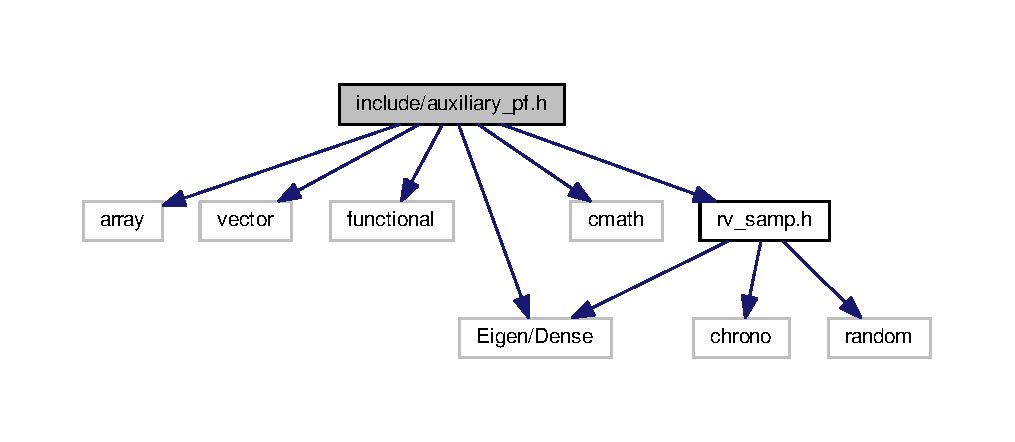
\includegraphics[width=350pt]{auxiliary__pf_8h__incl}
\end{center}
\end{figure}
\subsection*{Classes}
\begin{DoxyCompactItemize}
\item 
class \hyperlink{classAPF}{A\+P\+F$<$ nparts, dimx, dimy, resamp\+T $>$}
\begin{DoxyCompactList}\small\item\em A base-\/class for Auxiliary Particle Filtering. Filtering only, no smoothing. \end{DoxyCompactList}\end{DoxyCompactItemize}


\subsection{Detailed Description}
A base class for Auxiliary Particle Filtering. Inherit from this if you want to use an \hyperlink{classAPF}{A\+PF} for your state space model. Filtering only, no smoothing. 


\begin{DoxyTemplParams}{Template Parameters}
{\em nparts} & the number of particles \\
\hline
{\em dimx} & the dimension of the state \\
\hline
{\em dimy} & the dimension of the observations \\
\hline
{\em resampT} & the resampler type \\
\hline
\end{DoxyTemplParams}

\hypertarget{bootstrap__filter_8h}{}\section{include/pf/bootstrap\+\_\+filter.h File Reference}
\label{bootstrap__filter_8h}\index{include/pf/bootstrap\+\_\+filter.\+h@{include/pf/bootstrap\+\_\+filter.\+h}}


bootstrap particle filter  


{\ttfamily \#include $<$array$>$}\newline
{\ttfamily \#include $<$vector$>$}\newline
{\ttfamily \#include $<$Eigen/\+Dense$>$}\newline
{\ttfamily \#include \char`\"{}pf\+\_\+base.\+h\char`\"{}}\newline
Include dependency graph for bootstrap\+\_\+filter.\+h\+:\nopagebreak
\begin{figure}[H]
\begin{center}
\leavevmode
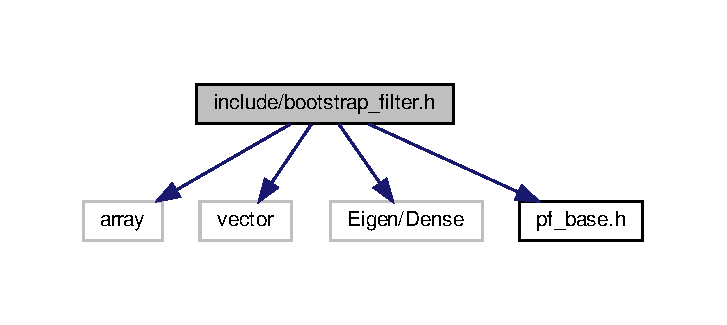
\includegraphics[width=350pt]{bootstrap__filter_8h__incl}
\end{center}
\end{figure}
\subsection*{Classes}
\begin{DoxyCompactItemize}
\item 
class \hyperlink{classBSFilter}{B\+S\+Filter$<$ nparts, dimx, dimy, resamp\+\_\+t, float\+\_\+t, debug $>$}
\begin{DoxyCompactList}\small\item\em A base class for the bootstrap particle filter. \end{DoxyCompactList}\end{DoxyCompactItemize}


\subsection{Detailed Description}
bootstrap particle filter 


\begin{DoxyTemplParams}{Template Parameters}
{\em nparts} & the number of particles \\
\hline
{\em dimx} & the dimension of the state \\
\hline
{\em dimy} & the dimension of the observations \\
\hline
{\em resamp\+\_\+t} & the type of resampler \\
\hline
\end{DoxyTemplParams}

\hypertarget{bootstrap__filter__with__covariates_8h}{}\section{include/bootstrap\+\_\+filter\+\_\+with\+\_\+covariates.h File Reference}
\label{bootstrap__filter__with__covariates_8h}\index{include/bootstrap\+\_\+filter\+\_\+with\+\_\+covariates.\+h@{include/bootstrap\+\_\+filter\+\_\+with\+\_\+covariates.\+h}}


bootstrap particle filter with covariates  


{\ttfamily \#include $<$array$>$}\newline
{\ttfamily \#include $<$vector$>$}\newline
{\ttfamily \#include $<$Eigen/\+Dense$>$}\newline
{\ttfamily \#include \char`\"{}pf\+\_\+base.\+h\char`\"{}}\newline
Include dependency graph for bootstrap\+\_\+filter\+\_\+with\+\_\+covariates.\+h\+:\nopagebreak
\begin{figure}[H]
\begin{center}
\leavevmode
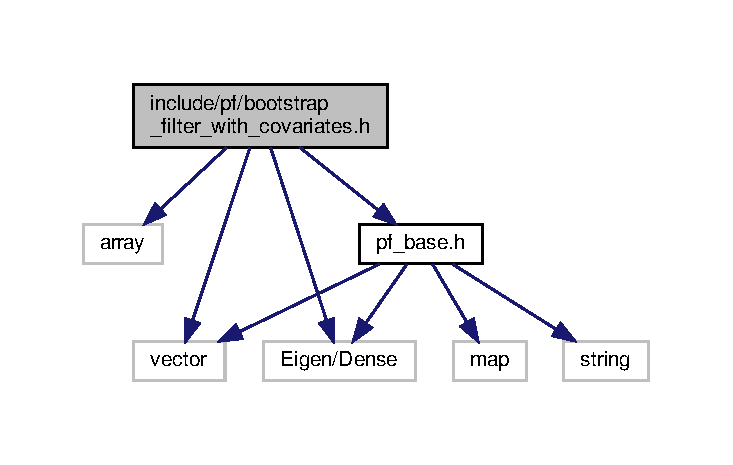
\includegraphics[width=350pt]{bootstrap__filter__with__covariates_8h__incl}
\end{center}
\end{figure}
\subsection*{Classes}
\begin{DoxyCompactItemize}
\item 
class \hyperlink{classBSFilterWC}{B\+S\+Filter\+W\+C$<$ nparts, dimx, dimy, dimcov, resamp\+\_\+t, float\+\_\+t $>$}
\begin{DoxyCompactList}\small\item\em A base class for the bootstrap particle filter with covariates. \end{DoxyCompactList}\end{DoxyCompactItemize}


\subsection{Detailed Description}
bootstrap particle filter with covariates 


\begin{DoxyTemplParams}{Template Parameters}
{\em nparts} & the number of particles \\
\hline
{\em dimx} & the dimension of the state \\
\hline
{\em dimy} & the dimension of the observations \\
\hline
{\em dimcov} & the dimension of the covariates \\
\hline
{\em resamp\+\_\+t} & the type of resampler \\
\hline
\end{DoxyTemplParams}

\hypertarget{cf__filters_8h}{}\section{include/cf\+\_\+filters.h File Reference}
\label{cf__filters_8h}\index{include/cf\+\_\+filters.\+h@{include/cf\+\_\+filters.\+h}}


forces structure on the closed-\/form filters.  


{\ttfamily \#include $<$Eigen/\+Dense$>$}\newline
{\ttfamily \#include $<$math.\+h$>$}\newline
{\ttfamily \#include \char`\"{}rv\+\_\+eval.\+h\char`\"{}}\newline
Include dependency graph for cf\+\_\+filters.\+h\+:\nopagebreak
\begin{figure}[H]
\begin{center}
\leavevmode
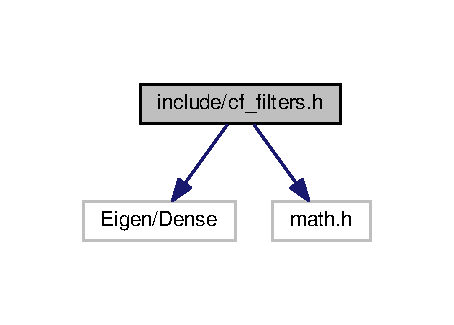
\includegraphics[width=350pt]{cf__filters_8h__incl}
\end{center}
\end{figure}
This graph shows which files directly or indirectly include this file\+:\nopagebreak
\begin{figure}[H]
\begin{center}
\leavevmode
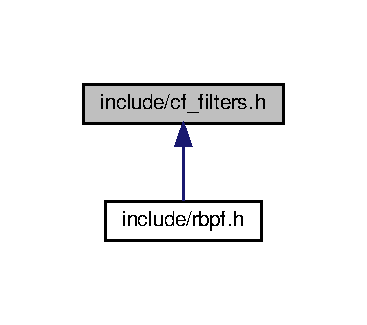
\includegraphics[width=176pt]{cf__filters_8h__dep__incl}
\end{center}
\end{figure}
\subsection*{Classes}
\begin{DoxyCompactItemize}
\item 
class \hyperlink{classcf__filter}{cf\+\_\+filter$<$ dimstate, dimobs, float\+\_\+t $>$}
\begin{DoxyCompactList}\small\item\em Abstract Base Class for all closed-\/form filters. \end{DoxyCompactList}\item 
class \hyperlink{classkalman}{kalman$<$ dimstate, dimobs, diminput, float\+\_\+t $>$}
\begin{DoxyCompactList}\small\item\em A class template for Kalman filtering. \end{DoxyCompactList}\item 
class \hyperlink{classhmm}{hmm$<$ dimstate, dimobs, float\+\_\+t $>$}
\begin{DoxyCompactList}\small\item\em A class template for H\+MM filtering. \end{DoxyCompactList}\item 
class \hyperlink{classgamFilter}{gam\+Filter$<$ dim\+\_\+pred, float\+\_\+t $>$}
\begin{DoxyCompactList}\small\item\em A class template for Gamma filtering. \end{DoxyCompactList}\item 
class \hyperlink{classmultivGamFilter}{multiv\+Gam\+Filter$<$ dim\+\_\+obs, dim\+\_\+pred, float\+\_\+t $>$}
\begin{DoxyCompactList}\small\item\em Another class template for Gamma filtering, but this time. \end{DoxyCompactList}\end{DoxyCompactItemize}


\subsection{Detailed Description}
forces structure on the closed-\/form filters. 

Inherit from this for a model that admits Gamma filtering.

Inherit from this for a model that admits H\+MM filtering.

Inherit from this for a model that admits Kalman filtering.
\hypertarget{pf__base_8h}{}\section{include/pf\+\_\+base.h File Reference}
\label{pf__base_8h}\index{include/pf\+\_\+base.\+h@{include/pf\+\_\+base.\+h}}


All non Rao-\/\+Blackwellized particle filters inherit from this.  


{\ttfamily \#include $<$map$>$}\newline
{\ttfamily \#include $<$string$>$}\newline
{\ttfamily \#include $<$vector$>$}\newline
{\ttfamily \#include $<$Eigen/\+Dense$>$}\newline
Include dependency graph for pf\+\_\+base.\+h\+:
\nopagebreak
\begin{figure}[H]
\begin{center}
\leavevmode
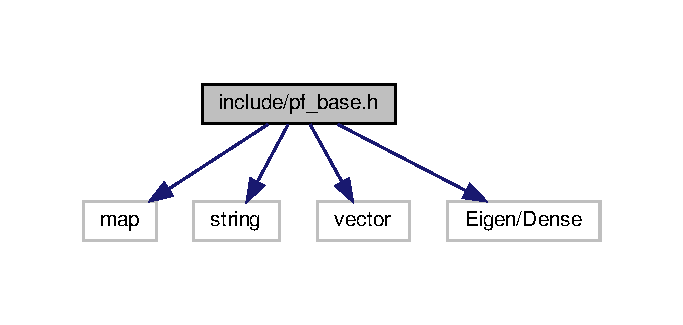
\includegraphics[width=328pt]{pf__base_8h__incl}
\end{center}
\end{figure}
This graph shows which files directly or indirectly include this file\+:
\nopagebreak
\begin{figure}[H]
\begin{center}
\leavevmode
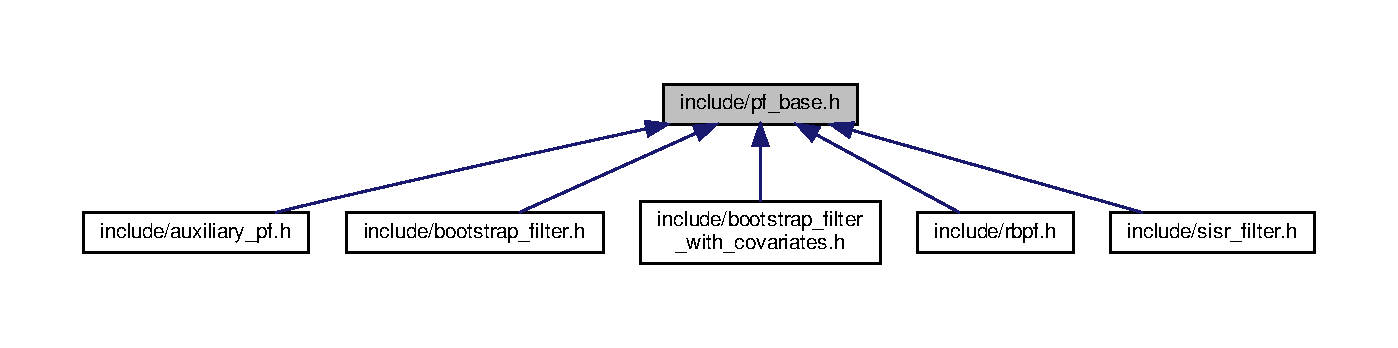
\includegraphics[width=350pt]{pf__base_8h__dep__incl}
\end{center}
\end{figure}
\subsection*{Classes}
\begin{DoxyCompactItemize}
\item 
class \hyperlink{classpf__base}{pf\+\_\+base$<$ float\+\_\+t, dimobs, dimstate $>$}
\item 
class \hyperlink{classrbpf__base}{rbpf\+\_\+base$<$ float\+\_\+t, dim\+\_\+s\+\_\+state, dim\+\_\+ns\+\_\+state, dimobs $>$}
\item 
class \hyperlink{classForwardMod}{Forward\+Mod$<$ dimx, dimy, float\+\_\+t $>$}
\end{DoxyCompactItemize}


\subsection{Detailed Description}
All non Rao-\/\+Blackwellized particle filters inherit from this. 

inherit from this if you want to simulate from a homogeneous forward/generative model.

All Rao-\/\+Blackwellized particle filters inherit from this.

\begin{DoxyAuthor}{Author}
t
\end{DoxyAuthor}

\begin{DoxyTemplParams}{Template Parameters}
{\em float\+\_\+t} & (e.\+g. double, float, etc.) \\
\hline
{\em dimobs} & the dimension of each observation \\
\hline
{\em dimstate} & the dimension of each state\\
\hline
\end{DoxyTemplParams}
\begin{DoxyAuthor}{Author}
t
\end{DoxyAuthor}

\begin{DoxyTemplParams}{Template Parameters}
{\em float\+\_\+t} & (e.\+g. double, float, etc.) \\
\hline
{\em dim\+\_\+s\+\_\+state} & the dimension of the state vector that\textquotesingle{}s sampled \\
\hline
{\em dim\+\_\+ns\+\_\+state} & the dimension of the state vector that isn\textquotesingle{}t sampled \\
\hline
{\em dimobs} & the dimension of each observation vector\\
\hline
\end{DoxyTemplParams}

\hypertarget{rbpf_8h}{}\section{include/pf/rbpf.h File Reference}
\label{rbpf_8h}\index{include/pf/rbpf.\+h@{include/pf/rbpf.\+h}}


Rao-\/\+Blackwellized/\+Marginal Particle Filter with inner H\+M\+Ms.  


{\ttfamily \#include $<$functional$>$}\newline
{\ttfamily \#include $<$vector$>$}\newline
{\ttfamily \#include $<$array$>$}\newline
{\ttfamily \#include $<$Eigen/\+Dense$>$}\newline
{\ttfamily \#include $<$algorithm$>$}\newline
{\ttfamily \#include \char`\"{}pf\+\_\+base.\+h\char`\"{}}\newline
{\ttfamily \#include \char`\"{}cf\+\_\+filters.\+h\char`\"{}}\newline
Include dependency graph for rbpf.\+h\+:\nopagebreak
\begin{figure}[H]
\begin{center}
\leavevmode
\includegraphics[width=350pt]{rbpf_8h__incl}
\end{center}
\end{figure}
\subsection*{Classes}
\begin{DoxyCompactItemize}
\item 
class \hyperlink{classrbpf__hmm}{rbpf\+\_\+hmm$<$ nparts, dimnss, dimss, dimy, resamp\+\_\+t, float\+\_\+t $>$}
\begin{DoxyCompactList}\small\item\em Rao-\/\+Blackwellized/\+Marginal Particle Filter with inner H\+M\+Ms. \end{DoxyCompactList}\item 
class \hyperlink{classrbpf__hmm__bs}{rbpf\+\_\+hmm\+\_\+bs$<$ nparts, dimnss, dimss, dimy, resamp\+\_\+t, float\+\_\+t $>$}
\begin{DoxyCompactList}\small\item\em Rao-\/\+Blackwellized/\+Marginal Bootstrap Filter with inner H\+M\+Ms. \end{DoxyCompactList}\item 
class \hyperlink{classrbpf__kalman}{rbpf\+\_\+kalman$<$ nparts, dimnss, dimss, dimy, resamp\+\_\+t, float\+\_\+t $>$}
\begin{DoxyCompactList}\small\item\em Rao-\/\+Blackwellized/\+Marginal Particle Filter with inner Kalman Filter objectss. \end{DoxyCompactList}\item 
class \hyperlink{classrbpf__kalman__bs}{rbpf\+\_\+kalman\+\_\+bs$<$ nparts, dimnss, dimss, dimy, resamp\+\_\+t, float\+\_\+t $>$}
\begin{DoxyCompactList}\small\item\em Rao-\/\+Blackwellized/\+Marginal Bootstrap Filter with inner Kalman Filter objectss. \end{DoxyCompactList}\end{DoxyCompactItemize}


\subsection{Detailed Description}
Rao-\/\+Blackwellized/\+Marginal Particle Filter with inner H\+M\+Ms. 

Rao-\/\+Blackwellized/\+Marginal Bootstrap Filter with inner Kalman Filter objectss.

Rao-\/\+Blackwellized/\+Marginal Particle Filter with inner Kalman Filter objectss.

Rao-\/\+Blackwellized/\+Marginal Bootstrap Filter with inner H\+M\+Ms.


\begin{DoxyTemplParams}{Template Parameters}
{\em nparts} & the number of particles \\
\hline
{\em dimnss} & dimension of \char`\"{}not sampled state\char`\"{} \\
\hline
{\em dimss} & dimension of \char`\"{}sampled state\char`\"{} \\
\hline
{\em dimy} & the dimension of the observations \\
\hline
{\em resamp\+\_\+t} & the resampler type (e.\+g. multinomial, etc.)\\
\hline
{\em nparts} & the number of particles \\
\hline
{\em dimnss} & dimension of not-\/sampled-\/state vector \\
\hline
{\em dimss} & dimension of sampled-\/state vector \\
\hline
{\em dimy} & the dimension of the observations \\
\hline
{\em resamp\+\_\+t} & the resampler type \\
\hline
\end{DoxyTemplParams}

\hypertarget{resamplers_8h}{}\section{include/pf/resamplers.h File Reference}
\label{resamplers_8h}\index{include/pf/resamplers.\+h@{include/pf/resamplers.\+h}}


all resamplers must inherit from this. This will enforce certain structure that are assumed by all particle filters.  


{\ttfamily \#include $<$chrono$>$}\newline
{\ttfamily \#include $<$array$>$}\newline
{\ttfamily \#include $<$random$>$}\newline
{\ttfamily \#include $<$numeric$>$}\newline
{\ttfamily \#include $<$cmath$>$}\newline
{\ttfamily \#include $<$Eigen/\+Dense$>$}\newline
Include dependency graph for resamplers.\+h\+:
\nopagebreak
\begin{figure}[H]
\begin{center}
\leavevmode
\includegraphics[width=350pt]{resamplers_8h__incl}
\end{center}
\end{figure}
\subsection*{Classes}
\begin{DoxyCompactItemize}
\item 
class \hyperlink{classrbase}{rbase$<$ nparts, dimx, float\+\_\+t $>$}
\begin{DoxyCompactList}\small\item\em Base class for all resampler types. \end{DoxyCompactList}\item 
class \hyperlink{classmn__resampler}{mn\+\_\+resampler$<$ nparts, dimx, float\+\_\+t $>$}
\item 
class \hyperlink{classmn__resampler__rbpf}{mn\+\_\+resampler\+\_\+rbpf$<$ nparts, dimsampledx, cf\+Mod\+T, float\+\_\+t $>$}
\item 
class \hyperlink{classresid__resampler}{resid\+\_\+resampler$<$ nparts, dimx, float\+\_\+t $>$}
\item 
class \hyperlink{classstratif__resampler}{stratif\+\_\+resampler$<$ nparts, dimx, float\+\_\+t $>$}
\item 
class \hyperlink{classsystematic__resampler}{systematic\+\_\+resampler$<$ nparts, dimx, float\+\_\+t $>$}
\item 
class \hyperlink{classmn__resamp__fast1}{mn\+\_\+resamp\+\_\+fast1$<$ nparts, dimx, float\+\_\+t $>$}
\end{DoxyCompactItemize}


\subsection{Detailed Description}
all resamplers must inherit from this. This will enforce certain structure that are assumed by all particle filters. 

Class that performs multinomial resampling for \char`\"{}standard\char`\"{} models. For justification, see page 244 of \char`\"{}\+Inference in Hidden Markov Models\char`\"{}.

Class that performs systematic resampling on \char`\"{}standard\char`\"{} models.

Class that performs stratified resampling on \char`\"{}standard\char`\"{} models.

Class that performs residual resampling on \char`\"{}standard\char`\"{} models.

Class that performs multinomial resampling for R\+B\+P\+Fs.

Class that performs multinomial resampling for \char`\"{}standard\char`\"{} models.


\begin{DoxyTemplParams}{Template Parameters}
{\em nparts} & the number of particles. \\
\hline
{\em dimx} & the dimension of each state sample.\\
\hline
{\em nparts} & the number of particles. \\
\hline
{\em dimsampledx} & the dimension of each state sample. \\
\hline
{\em cf\+ModT} & the type of closed form model \\
\hline
{\em float\+\_\+t} & the type of floating point number\\
\hline
{\em nparts} & the number of particles. \\
\hline
{\em dimx} & the dimension of each state sample. \\
\hline
{\em float\+\_\+t} & the floating point for samples \\
\hline
\end{DoxyTemplParams}

\hypertarget{rv__samp_8h}{}\section{include/pf/rv\+\_\+samp.h File Reference}
\label{rv__samp_8h}\index{include/pf/rv\+\_\+samp.\+h@{include/pf/rv\+\_\+samp.\+h}}


all rv samplers must inherit from this.  


{\ttfamily \#include $<$chrono$>$}\newline
{\ttfamily \#include $<$Eigen/\+Dense$>$}\newline
{\ttfamily \#include $<$random$>$}\newline
Include dependency graph for rv\+\_\+samp.\+h\+:
\nopagebreak
\begin{figure}[H]
\begin{center}
\leavevmode
\includegraphics[width=285pt]{rv__samp_8h__incl}
\end{center}
\end{figure}
This graph shows which files directly or indirectly include this file\+:
\nopagebreak
\begin{figure}[H]
\begin{center}
\leavevmode
\includegraphics[width=199pt]{rv__samp_8h__dep__incl}
\end{center}
\end{figure}
\subsection*{Classes}
\begin{DoxyCompactItemize}
\item 
class \hyperlink{classrvsamp_1_1rvsamp__base}{rvsamp\+::rvsamp\+\_\+base}
\begin{DoxyCompactList}\small\item\em Base class for all random variable sampler types. Primary benefit is that it sets the seed for you. \end{DoxyCompactList}\item 
class \hyperlink{classrvsamp_1_1UnivNormSampler}{rvsamp\+::\+Univ\+Norm\+Sampler$<$ float\+\_\+t $>$}
\begin{DoxyCompactList}\small\item\em A class that performs sampling from a univariate Normal distribution. \end{DoxyCompactList}\item 
class \hyperlink{classrvsamp_1_1UnivLogNormSampler}{rvsamp\+::\+Univ\+Log\+Norm\+Sampler$<$ float\+\_\+t $>$}
\begin{DoxyCompactList}\small\item\em A class that performs sampling from a univariate Log-\/\+Normal distribution. \end{DoxyCompactList}\item 
class \hyperlink{classrvsamp_1_1UnivGammaSampler}{rvsamp\+::\+Univ\+Gamma\+Sampler$<$ float\+\_\+t $>$}
\begin{DoxyCompactList}\small\item\em A class that performs sampling from a univariate Gamma distribution. \end{DoxyCompactList}\item 
class \hyperlink{classrvsamp_1_1UnivInvGammaSampler}{rvsamp\+::\+Univ\+Inv\+Gamma\+Sampler$<$ float\+\_\+t $>$}
\begin{DoxyCompactList}\small\item\em A class that performs sampling from a univariate Inverse Gamma distribution. \end{DoxyCompactList}\item 
class \hyperlink{classrvsamp_1_1TruncUnivNormSampler}{rvsamp\+::\+Trunc\+Univ\+Norm\+Sampler$<$ float\+\_\+t $>$}
\begin{DoxyCompactList}\small\item\em A class that performs sampling from a truncated univariate Normal distribution. \end{DoxyCompactList}\item 
class \hyperlink{classrvsamp_1_1PoissonSampler}{rvsamp\+::\+Poisson\+Sampler$<$ float\+\_\+t, int\+\_\+t $>$}
\begin{DoxyCompactList}\small\item\em A class that performs sampling from a Poisson distribution. \end{DoxyCompactList}\item 
class \hyperlink{classrvsamp_1_1BernSampler}{rvsamp\+::\+Bern\+Sampler$<$ float\+\_\+t, int\+\_\+t $>$}
\begin{DoxyCompactList}\small\item\em A class that performs sampling from a univariate Bernoulli distribution. \end{DoxyCompactList}\item 
class \hyperlink{classrvsamp_1_1MVNSampler}{rvsamp\+::\+M\+V\+N\+Sampler$<$ dim, float\+\_\+t $>$}
\begin{DoxyCompactList}\small\item\em A class that performs sampling from a multivariate normal distribution. \end{DoxyCompactList}\item 
class \hyperlink{classrvsamp_1_1UniformSampler}{rvsamp\+::\+Uniform\+Sampler$<$ float\+\_\+t $>$}
\begin{DoxyCompactList}\small\item\em A class that performs sampling from a continuous uniform distribution. \end{DoxyCompactList}\item 
class \hyperlink{classrvsamp_1_1k__gen}{rvsamp\+::k\+\_\+gen$<$ N, float\+\_\+t $>$}
\begin{DoxyCompactList}\small\item\em A class that performs sampling with replacement (useful for the index sampler in an \hyperlink{classAPF}{A\+PF}) \end{DoxyCompactList}\end{DoxyCompactItemize}


\subsection{Detailed Description}
all rv samplers must inherit from this. 

Basically a wrapper for std\+::discrete\+\_\+distribution$<$$>$ outputs are in the rage (0,1,...N-\/1)

Can sample from a distribution with fixed mean and covariance, fixed mean only, fixed covariance only, or nothing fixed.

Samples from univariate Bernoulli distribution.

Samples from univariate Poisson distribution.

Samples from a truncated univariate Normal distribution using the acceptance rejection method. The proposal distribution used is a normal distribution with the same location and scale parameters as the target. As a result, this method will take a long time when the width of the support of the target is narrow.

Samples from univariate Inverse Gamma distribution.

Samples from univariate Gamma distribution.

Samples from univariate Log-\/\+Normal distribution.

Samples from univariate Normal distribution.


\begin{DoxyTemplParams}{Template Parameters}
{\em dim} & the dimension of each random vector sample.\\
\hline
\end{DoxyTemplParams}

\hypertarget{sisr__filter_8h}{}\section{include/pf/sisr\+\_\+filter.h File Reference}
\label{sisr__filter_8h}\index{include/pf/sisr\+\_\+filter.\+h@{include/pf/sisr\+\_\+filter.\+h}}


S\+I\+SR filter.  


{\ttfamily \#include $<$array$>$}\newline
{\ttfamily \#include $<$Eigen/\+Dense$>$}\newline
{\ttfamily \#include \char`\"{}pf\+\_\+base.\+h\char`\"{}}\newline
Include dependency graph for sisr\+\_\+filter.\+h\+:\nopagebreak
\begin{figure}[H]
\begin{center}
\leavevmode
\includegraphics[width=350pt]{sisr__filter_8h__incl}
\end{center}
\end{figure}
\subsection*{Classes}
\begin{DoxyCompactItemize}
\item 
class \hyperlink{classSISRFilter}{S\+I\+S\+R\+Filter$<$ nparts, dimx, dimy, resamp\+\_\+t, float\+\_\+t, debug $>$}
\begin{DoxyCompactList}\small\item\em A base class for the Sequential Important Sampling with Resampling (S\+I\+SR). \end{DoxyCompactList}\end{DoxyCompactItemize}


\subsection{Detailed Description}
S\+I\+SR filter. 


\begin{DoxyTemplParams}{Template Parameters}
{\em nparts} & the number of particles \\
\hline
{\em dimx} & the size of the state \\
\hline
{\em the} & size of the observation \\
\hline
{\em resamp\+\_\+t} & the type of resampler \\
\hline
\end{DoxyTemplParams}

%--- End generated contents ---

% Index
\backmatter
\newpage
\phantomsection
\clearemptydoublepage
\addcontentsline{toc}{chapter}{Index}
\printindex

\end{document}
